\documentclass[]{book}
\usepackage{lmodern}
\usepackage{amssymb,amsmath}
\usepackage{ifxetex,ifluatex}
\usepackage{fixltx2e} % provides \textsubscript
\ifnum 0\ifxetex 1\fi\ifluatex 1\fi=0 % if pdftex
  \usepackage[T1]{fontenc}
  \usepackage[utf8]{inputenc}
\else % if luatex or xelatex
  \ifxetex
    \usepackage{mathspec}
  \else
    \usepackage{fontspec}
  \fi
  \defaultfontfeatures{Ligatures=TeX,Scale=MatchLowercase}
\fi
% use upquote if available, for straight quotes in verbatim environments
\IfFileExists{upquote.sty}{\usepackage{upquote}}{}
% use microtype if available
\IfFileExists{microtype.sty}{%
\usepackage{microtype}
\UseMicrotypeSet[protrusion]{basicmath} % disable protrusion for tt fonts
}{}
\usepackage{hyperref}
\hypersetup{unicode=true,
            pdftitle={CM 1110 Fundamentals of Mathematics and Statistics},
            pdfauthor={Dr.~Priyanga D. Talagala},
            pdfborder={0 0 0},
            breaklinks=true}
\urlstyle{same}  % don't use monospace font for urls
\usepackage{natbib}
\bibliographystyle{apalike}
\usepackage{longtable,booktabs}
\usepackage{graphicx,grffile}
\makeatletter
\def\maxwidth{\ifdim\Gin@nat@width>\linewidth\linewidth\else\Gin@nat@width\fi}
\def\maxheight{\ifdim\Gin@nat@height>\textheight\textheight\else\Gin@nat@height\fi}
\makeatother
% Scale images if necessary, so that they will not overflow the page
% margins by default, and it is still possible to overwrite the defaults
% using explicit options in \includegraphics[width, height, ...]{}
\setkeys{Gin}{width=\maxwidth,height=\maxheight,keepaspectratio}
\IfFileExists{parskip.sty}{%
\usepackage{parskip}
}{% else
\setlength{\parindent}{0pt}
\setlength{\parskip}{6pt plus 2pt minus 1pt}
}
\setlength{\emergencystretch}{3em}  % prevent overfull lines
\providecommand{\tightlist}{%
  \setlength{\itemsep}{0pt}\setlength{\parskip}{0pt}}
\setcounter{secnumdepth}{5}
% Redefines (sub)paragraphs to behave more like sections
\ifx\paragraph\undefined\else
\let\oldparagraph\paragraph
\renewcommand{\paragraph}[1]{\oldparagraph{#1}\mbox{}}
\fi
\ifx\subparagraph\undefined\else
\let\oldsubparagraph\subparagraph
\renewcommand{\subparagraph}[1]{\oldsubparagraph{#1}\mbox{}}
\fi

%%% Use protect on footnotes to avoid problems with footnotes in titles
\let\rmarkdownfootnote\footnote%
\def\footnote{\protect\rmarkdownfootnote}

%%% Change title format to be more compact
\usepackage{titling}

% Create subtitle command for use in maketitle
\providecommand{\subtitle}[1]{
  \posttitle{
    \begin{center}\large#1\end{center}
    }
}

\setlength{\droptitle}{-2em}

  \title{CM 1110 Fundamentals of Mathematics and Statistics}
    \pretitle{\vspace{\droptitle}\centering\huge}
  \posttitle{\par}
    \author{Dr.~Priyanga D. Talagala}
    \preauthor{\centering\large\emph}
  \postauthor{\par}
      \predate{\centering\large\emph}
  \postdate{\par}
    \date{2020-03-11}

\usepackage{booktabs}
\usepackage{amsthm}
\makeatletter
\def\thm@space@setup{%
  \thm@preskip=8pt plus 2pt minus 4pt
  \thm@postskip=\thm@preskip
}
\makeatother

\begin{document}
\maketitle

{
\setcounter{tocdepth}{1}
\tableofcontents
}
\hypertarget{course-syllabus}{%
\chapter*{Course Syllabus}\label{course-syllabus}}
\addcontentsline{toc}{chapter}{Course Syllabus}

\hypertarget{pre-requisites}{%
\section*{Pre-requisites}\label{pre-requisites}}
\addcontentsline{toc}{section}{Pre-requisites}

None

\hypertarget{learning-outcomes}{%
\section*{Learning Outcomes}\label{learning-outcomes}}
\addcontentsline{toc}{section}{Learning Outcomes}

On successful completion of this module, students will be able to apply fundamental concepts in Mathematics and Statistics for real world problem solving.

\hypertarget{outline-syllabus}{%
\section*{Outline Syllabus}\label{outline-syllabus}}
\addcontentsline{toc}{section}{Outline Syllabus}

\begin{itemize}
\tightlist
\item
  Number Systems
\item
  Sequences and Series
\item
  Introduction to Logic
\item
  Boolean Algebra
\item
  Differentiation and Integration
\item
  Descriptive Statistics
\item
  Sets and Relations
\item
  Probability
\item
  Correlation and Regression
\end{itemize}

\hypertarget{method-of-assessment}{%
\section*{Method of Assessment}\label{method-of-assessment}}
\addcontentsline{toc}{section}{Method of Assessment}

\begin{itemize}
\tightlist
\item
  Mid-semester examination
\item
  End-semester examination
\end{itemize}

\hypertarget{lecturer}{%
\section*{Lecturer}\label{lecturer}}
\addcontentsline{toc}{section}{Lecturer}

Dr.~Priyanga D. Talagala

\hypertarget{schedule}{%
\section*{Schedule}\label{schedule}}
\addcontentsline{toc}{section}{Schedule}

Lectures:

\begin{itemize}
\tightlist
\item
  Monday {[}1.15 pm - 4.30 pm{]}
\end{itemize}

Tutorial:

\begin{itemize}
\tightlist
\item
  Thursday {[}1.15 pm - 4.30 pm{]}
\end{itemize}

Consultation time:

\begin{itemize}
\tightlist
\item
  Tuesday {[}11.30 am to 12.30 pm{]}
\end{itemize}

\hypertarget{number-systems}{%
\chapter{Number Systems}\label{number-systems}}

\pagenumbering{arabic}

Numbers can be classified according to how they are represented or according to the properties that they have.

\hypertarget{main-types}{%
\section{Main types}\label{main-types}}

\begin{center}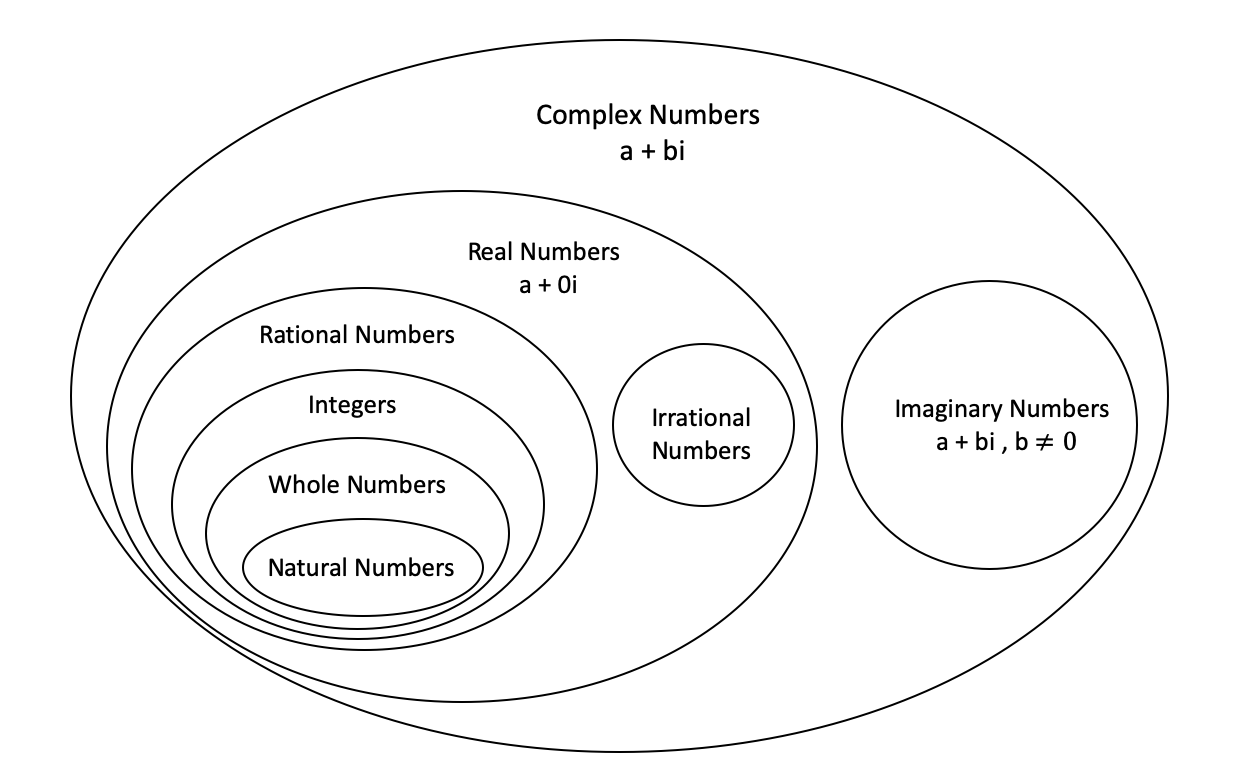
\includegraphics[width=1\linewidth]{figure/1-numbertypes} \end{center}

\hypertarget{complex-numbers}{%
\subsection{Complex numbers}\label{complex-numbers}}

\begin{itemize}
\tightlist
\item
  Every number in number system is considered as a complex number
\item
  A number of the form \(a+ib\) is called a complex number when \(a\) and \(b\) are real numbers and \(i=\sqrt{-1}\).
\item
  For a given complex number, \(a+ib\), `\(a\)' is known as the real part and `\(b\)' is known as the imaginary part.
\item
  If \(a=0\), the number \(ib\) is said to be purely imaginary, if \(b=0\) the number \(a\) is real.
\item
  A pair of complex number \(a+ib\) and \(a-ib\) are said to be conjugate of each other.
\end{itemize}

\textbf{Show that the sum and product of a complex number and its conjugate complex are both real.}

\begin{center}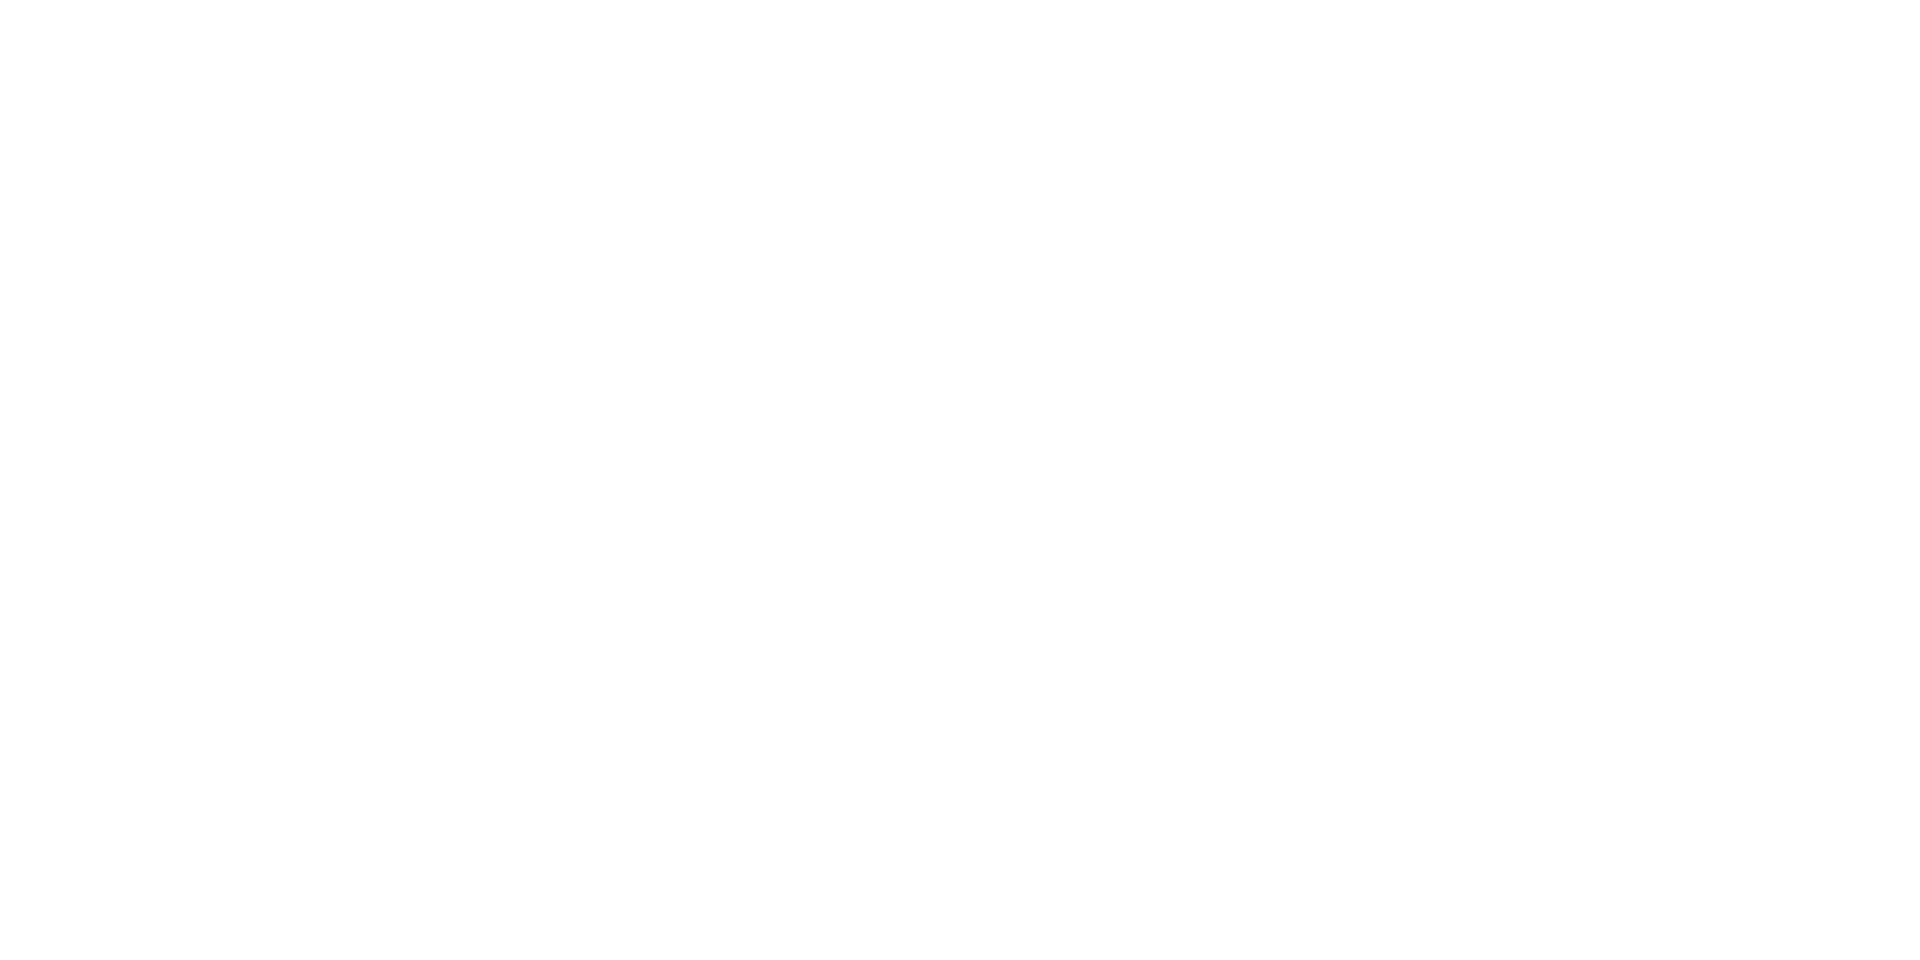
\includegraphics[width=1\linewidth]{figure/NSbox1a-1} \end{center}

\begin{itemize}
\tightlist
\item
  Let \(a+ib\) and \(c+id\) be two complex numbers. Then
\end{itemize}

\textbf{Addition.} \((a+ib) + (c+id)= (a+c)+i(b+d)\)

\textbf{Subtraction} \((a+ib) - (c+id)= (a-c)+i(b-d)\)

\textbf{Multiplication} \((a+ib) \times (c+id)= ac-bd+i(ad+bc)\)

\textbf{Addition.} \(\frac{a+ib}{c+id}= \frac{a+ib}{c+id}.\frac{c-id}{c-id}= \frac{ac+bd}{c^2+d^2}+i\frac{bc-ad}{c^2+d^2}\)

\begin{itemize}
\tightlist
\item
  Complex numbers are denoted by \(\mathbb{C}\).
\end{itemize}

\hypertarget{imaginary-numbers}{%
\subsection{Imaginary numbers}\label{imaginary-numbers}}

\begin{itemize}
\tightlist
\item
  A number that does not exist in the number line is known as imaginary number.
\item
  For example, square root of negative numbers are imaginary numbers. It is denoted by \(i\).
  i.e \[\sqrt{-1}=i\] \newline
  \[i^{2} = – 1\]
\item
  So there is no real number \(i\) that satisfies the above equation.
\item
  The quantity, \(i\) is called the unit imaginary number.
\end{itemize}

\textbf{Geometrical Representation of imaginary numbers}

\begin{center}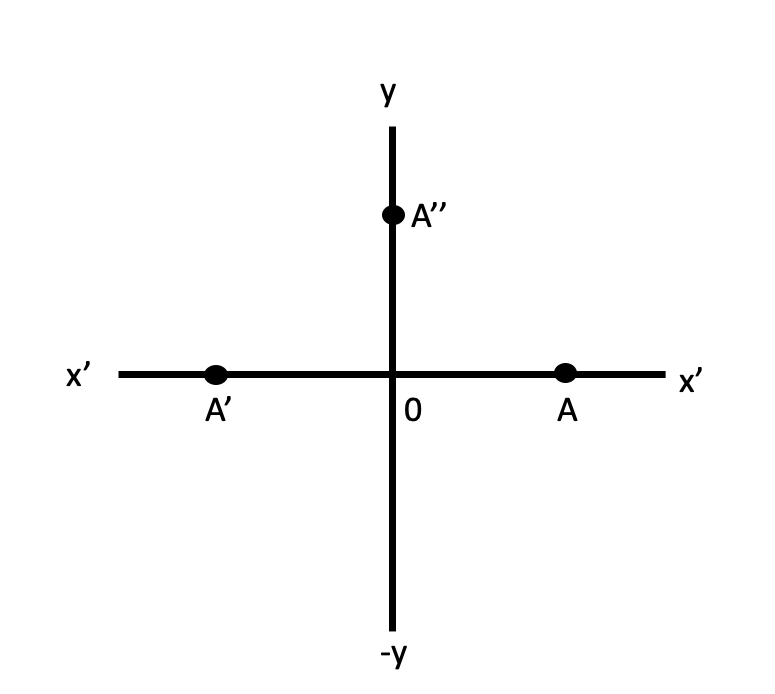
\includegraphics[width=0.5\linewidth]{figure/1-ImgNum} \end{center}

\begin{itemize}
\tightlist
\item
  Let OA be positive numbers which is represented by \(x\) and \(OA^\prime\) by \(-x\).
\item
  And \(-x= (i)^2x=i(ix)\) is on \(OX^{\prime}\).
\item
  According to the above expression, the multiplication of the real number \(x\) by \(i\) twice amounts is equivalent to the rotation of OA through two right angles to reach \(OA^\prime\).
\item
  Therefore, the multiplication of \(x\) by \(i\) is equivalent to the rotation of \(x\) through one right angle to reach \(OA^{\prime\prime}\).
\item
  Therefore, y-axis is known as imaginary axis.
\item
  Multiplication by \(i\) rotates its direction through right angle.
\end{itemize}

\hypertarget{real-numbers}{%
\subsection{Real numbers}\label{real-numbers}}

\begin{itemize}
\tightlist
\item
  All numbers that can be represented on the number line are known as real numbers.
\item
  The real numbers is the set of numbers containing all of the rational numbers and all of the irrational numbers.
\item
  Real Numbers are denoted by \(\mathbb{R}\).
\end{itemize}

\hypertarget{rational-numbers}{%
\subsection{Rational numbers}\label{rational-numbers}}

\begin{itemize}
\item
  Rational Numbers are denoted by \(\mathbb{Q}\)
\item
  A rational number is defined as number of the form \(x/y\) where \(x\) and \(y\) are integers and \(y \neq 0\).
\item
  The set of rational numbers encloses the set of integers and fractions.
\item
  The rational numbers that are not integral will have decimal values. These values can be of two types

  \begin{itemize}
  \tightlist
  \item
    Terminating decimal fractions (finite decimal factors): For example \(1/5 = 0.5\) , \(13/5 = 2.6\).
  \item
    Non Terminating decimal fractions. The non terminating decimal fractions having two types:

    \begin{enumerate}
    \def\labelenumi{\roman{enumi})}
    \tightlist
    \item
      Non terminating periodic fractions
    \item
      Non terminating non periodic fractions
    \end{enumerate}
  \end{itemize}
\end{itemize}

\emph{i) Non terminating periodic fractions}

\begin{enumerate}
\def\labelenumi{\alph{enumi}.}
\item
  These are non terminating decimal fractions of the type \(a.b1b2b3b4b5 .....bmb1b2b3b4b5 .....bm\)
\item
  Examples

  \(19/6 = 3.16666666.....\)

  \(18/7 = 2.57142857142857.......\)

  \(21/9= 2.3333.......\)
\end{enumerate}

\emph{ii) Non terminating non periodic fractions}

\begin{enumerate}
\def\labelenumi{\alph{enumi}.}
\tightlist
\item
  These are non terminating and there is no periodic decimal places for that number.
\item
  i.e \(a.b1b2b3b4b5 .....bmc1c2.........\)
\item
  for example 6.789542587436512\ldots{}\ldots{}\ldots{}.
\end{enumerate}

\begin{itemize}
\tightlist
\item
  \textbf{So from above terminating and non terminating periodic fraction numbers belongs to rational numbers.}
\end{itemize}

\hypertarget{irrational-numbers}{%
\subsection{Irrational numbers}\label{irrational-numbers}}

\begin{itemize}
\tightlist
\item
  Irrational numbers are denoted by \(\mathbb{I}\)
\item
  Irrational numbers are consisted with \textbf{non terminating and non periodic fractions}.
\item
  i.e irrational number is a number that cannot be written as a ratio \(x/y\) form (or fraction).
\item
  In decimal form, it never ends or repeats.
\item
  Examples for irrational numbers are \(\sqrt{2} = 1.414213......\), \(\pi = 3.14159265.......\), \(\sqrt{3}\), \(\sqrt{5}\) etc.
\end{itemize}

\hypertarget{integers}{%
\subsection{Integers}\label{integers}}

\begin{itemize}
\tightlist
\item
  All numbers that do not have the decimal places in them are called integers.
\item
  \(\mathbb{Z} = \{...,-5,-4,-3,-2,-1,0,1,2,3,4,5,...\}\)
\item
  i.e it may be positive or negative or zero.
\item
  Integers are denoted by \(\mathbb{Z}\).
\item
  Any integers are added, subtracted, or multiplied the result is always is an integer.
\item
  When any integers multiplied , each of the multiplied integer is called a factor or divisor of the resulting product.
\end{itemize}

\hypertarget{whole-numbers}{%
\subsection{Whole numbers}\label{whole-numbers}}

\begin{itemize}
\tightlist
\item
  The set of whole numbers means narrator numbers and \(0\)
\item
  Whole numbers = \(\mathbb{W} = \{ 0,1,2,3,4,5,6,7,8,...\}\)
\end{itemize}

\hypertarget{natural-numbers}{%
\subsection{Natural numbers}\label{natural-numbers}}

\begin{itemize}
\tightlist
\item
  The counting numbers start with 1 and their end is not defined.
\item
  i.e \(\mathbb{N} =\{1,2,3,4,...\}\)
\end{itemize}

\textbf{Reading :}

Dass, H. K. (2008). `Complex Numbers', \emph{Advanced Engineering Mathematics}. S. Chand Publishing. pp.~474-520.

\hypertarget{number-representations}{%
\section{Number representations}\label{number-representations}}

\hypertarget{glossary-of-terms-used-in-the-positional-numeral-systems}{%
\subsection{Glossary of terms used in the positional numeral systems}\label{glossary-of-terms-used-in-the-positional-numeral-systems}}

\begin{center}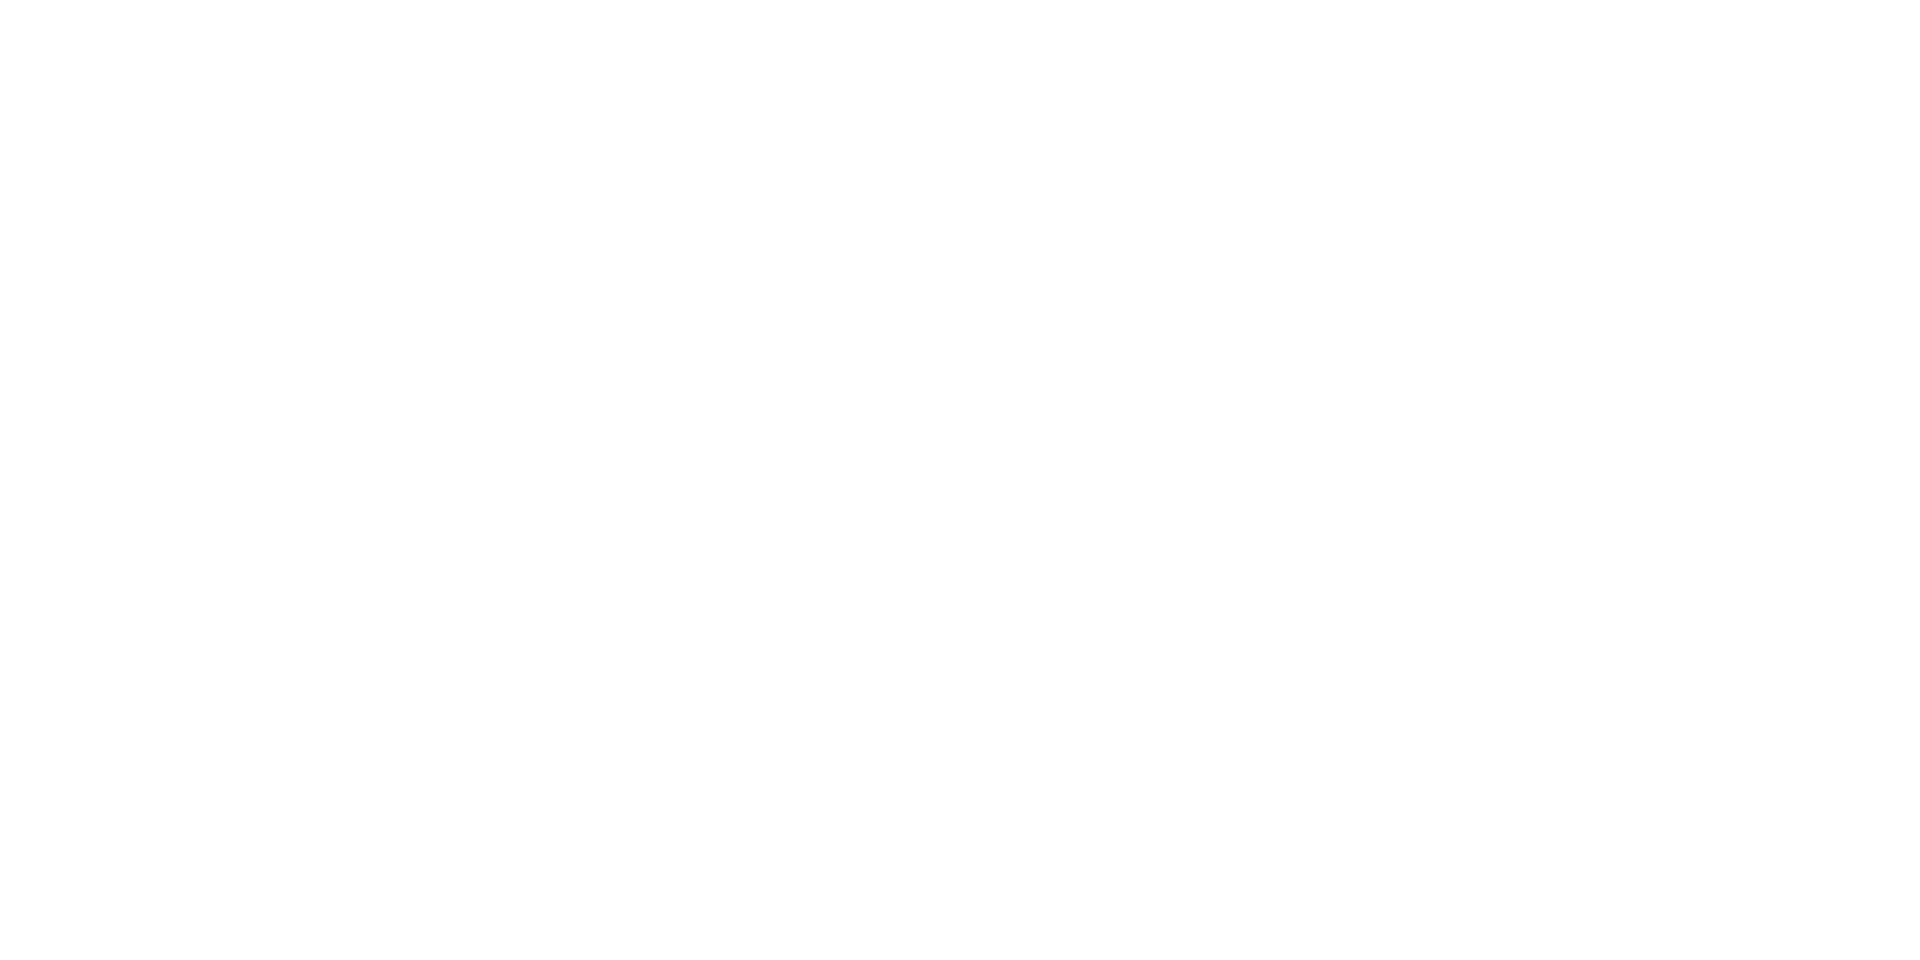
\includegraphics[width=1\linewidth]{figure/NSbox1-1} \end{center}

\begin{itemize}
\item
  There are various types of the number system in mathematics.
\item
  The four most common number system types are:

  \begin{itemize}
  \tightlist
  \item
    Decimal number system (Base- 10)
  \item
    Binary number system (Base- 2)
  \item
    Octal number system (Base-8)
  \item
    Hexadecimal number system (Base- 16)
  \end{itemize}
\end{itemize}

\begin{longtable}[]{@{}lll@{}}
\toprule
System & Radix/ Base & Digits\tabularnewline
\midrule
\endhead
Binary & 2 & 0 1\tabularnewline
Octal & 8 & 0 1 2 3 4 5 6 7\tabularnewline
Decimal & 10 & 0 1 2 3 4 5 6 7 8 9\tabularnewline
Hexadecimal & 16 & 0 1 2 3 4 5 6 7 8 9 A B C D E F\tabularnewline
\bottomrule
\end{longtable}

\hypertarget{decimal-number-system}{%
\subsection{Decimal Number System}\label{decimal-number-system}}

\begin{itemize}
\item
  The Decimal number system is a number of base or radix equal to 10.
\item
  To determine the actual number in each position, take the number that appears in the position and multiply it by \(10^x\), where \(x\) is the power representation.
\end{itemize}

\textbf{Example 1: The value of the combination of symbols 453 is determined by adding the weights of each position as}

\[4\times10^2+5\times10^1+3\times10^0\]
\[= 4\times100 + 5\times10+3\times1\]
Or \[= 400+50+3 = 453\]

\textbf{Example 2: The value of the combination of symbols 369.54 is determined by adding the weights of each position as}

\[3\times10^2+6\times10^1+9\times10^0+5\times10^{-1}+4\times10^{-2}\]
Or \[= 300 + 60+9+\frac{5}{10}+\frac{4}{100}\]
Or \[= 300 + 60+9+0.5+0.04= 369.54\]

\hypertarget{binary-number-system}{%
\subsection{Binary Number System}\label{binary-number-system}}

\begin{itemize}
\tightlist
\item
  The binary number system is a number system of base or radix equal to 2.
\item
  In the binary number system, there are two symbols to represent number: 0 and 1
\item
  When the symbols 0 an 1 are used to represent binary number, each symbol is called a binary digit or a bit.
\item
  Therefore, the binary number 1011 is a four-digit number or a 4-bit binary number.
\end{itemize}

\hypertarget{binary-to-decimal-conversion}{%
\subsubsection{Binary-to-Decimal Conversion}\label{binary-to-decimal-conversion}}

\begin{itemize}
\tightlist
\item
  Multiply binary digit (1 or 0) in each position by the weight of the position and add the results.
\end{itemize}

\textbf{Example 1: Convert the binary number 11010 to its decimal equivalent}

\begin{center}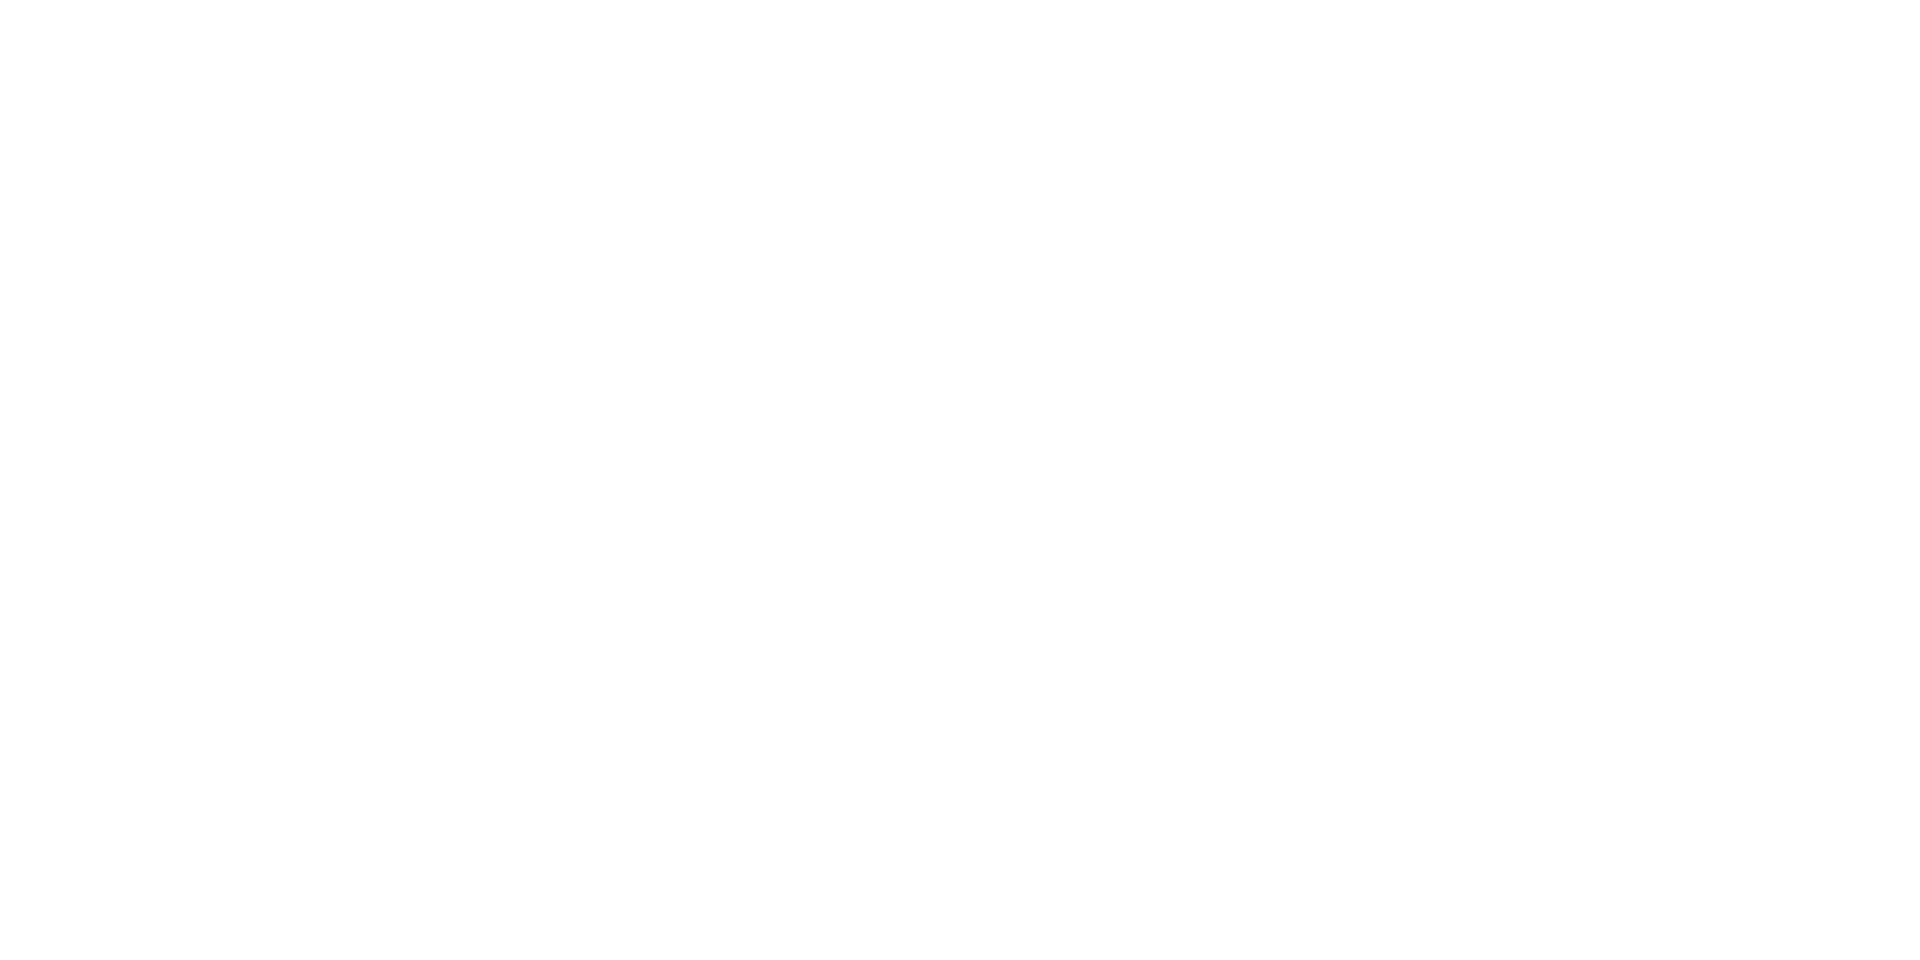
\includegraphics[width=1\linewidth]{figure/NSbox2-1} \end{center}

\textbf{Example 2: Convert the binary number 0.011 to its decimal equivalent}

\begin{center}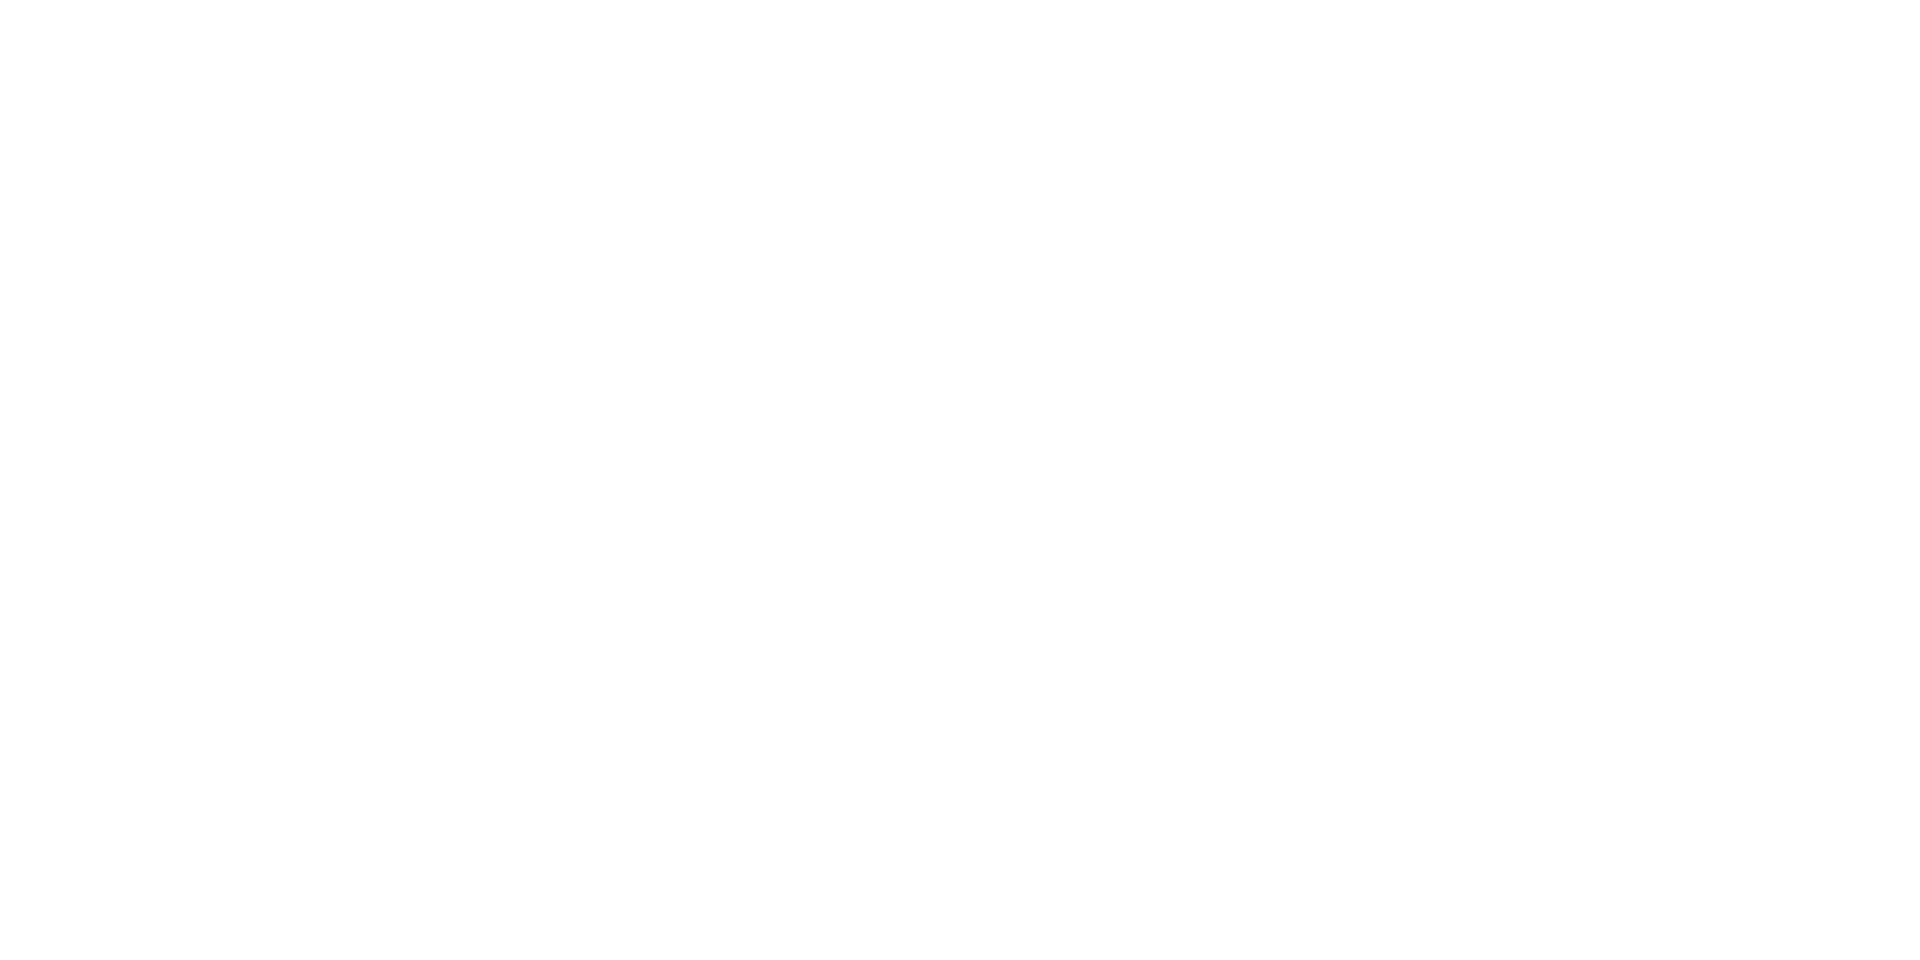
\includegraphics[width=1\linewidth]{figure/NSbox3-1} \end{center}

\textbf{Example 3: Convert the binary number 110.011 to its decimal equivalent}

\begin{center}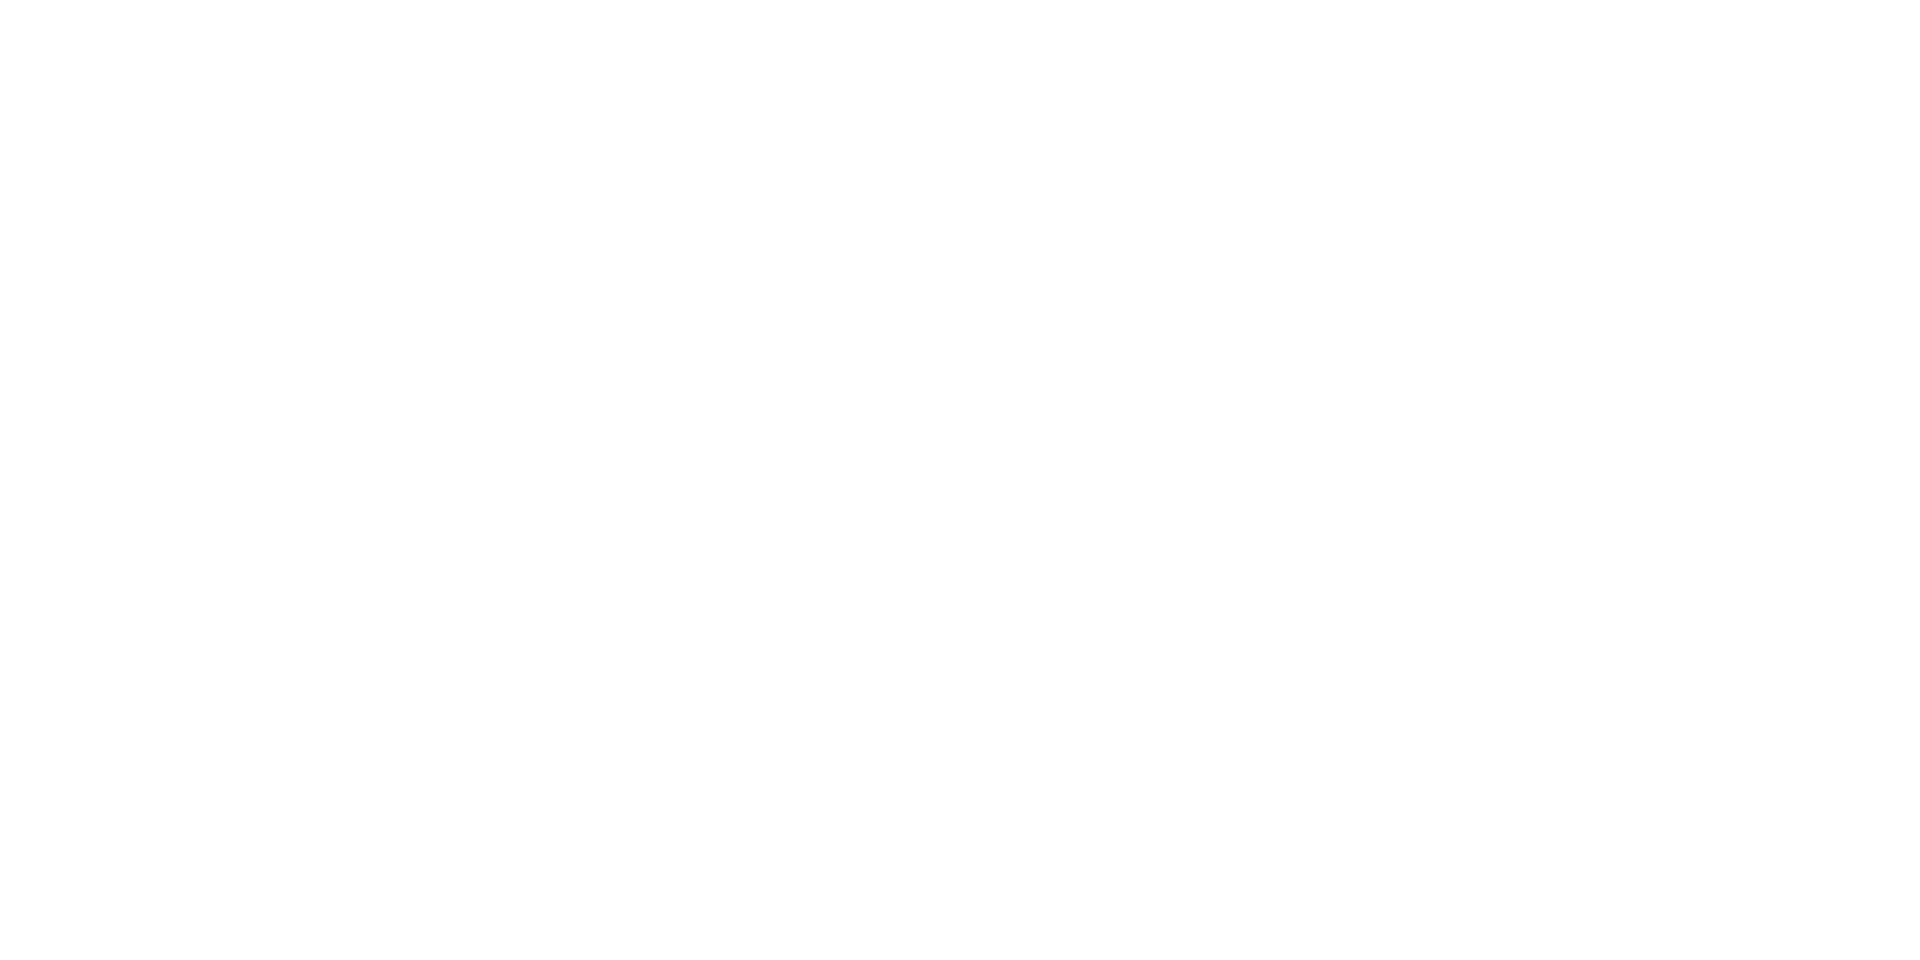
\includegraphics[width=1\linewidth]{figure/NSbox4-1} \end{center}

\hypertarget{decimal-to-binary-conversion}{%
\subsubsection{Decimal-to-Binary Conversion}\label{decimal-to-binary-conversion}}

\begin{itemize}
\tightlist
\item
  To convert decimal numbers to their binary equivalent, the following procedures are employed:
\end{itemize}

\hypertarget{whole-number-conversion-repeated-division-by-2}{%
\paragraph{Whole number conversion: Repeated division by 2}\label{whole-number-conversion-repeated-division-by-2}}

\begin{itemize}
\tightlist
\item
  The remainder resulting from each division forms binary number.
\item
  The first remainder to be produced is called the least significant bit (LSB) and the last remainder is called most significant bit (MSB).
\end{itemize}

\textbf{Example 1: Convert the decimal number 17 to binary}

\begin{center}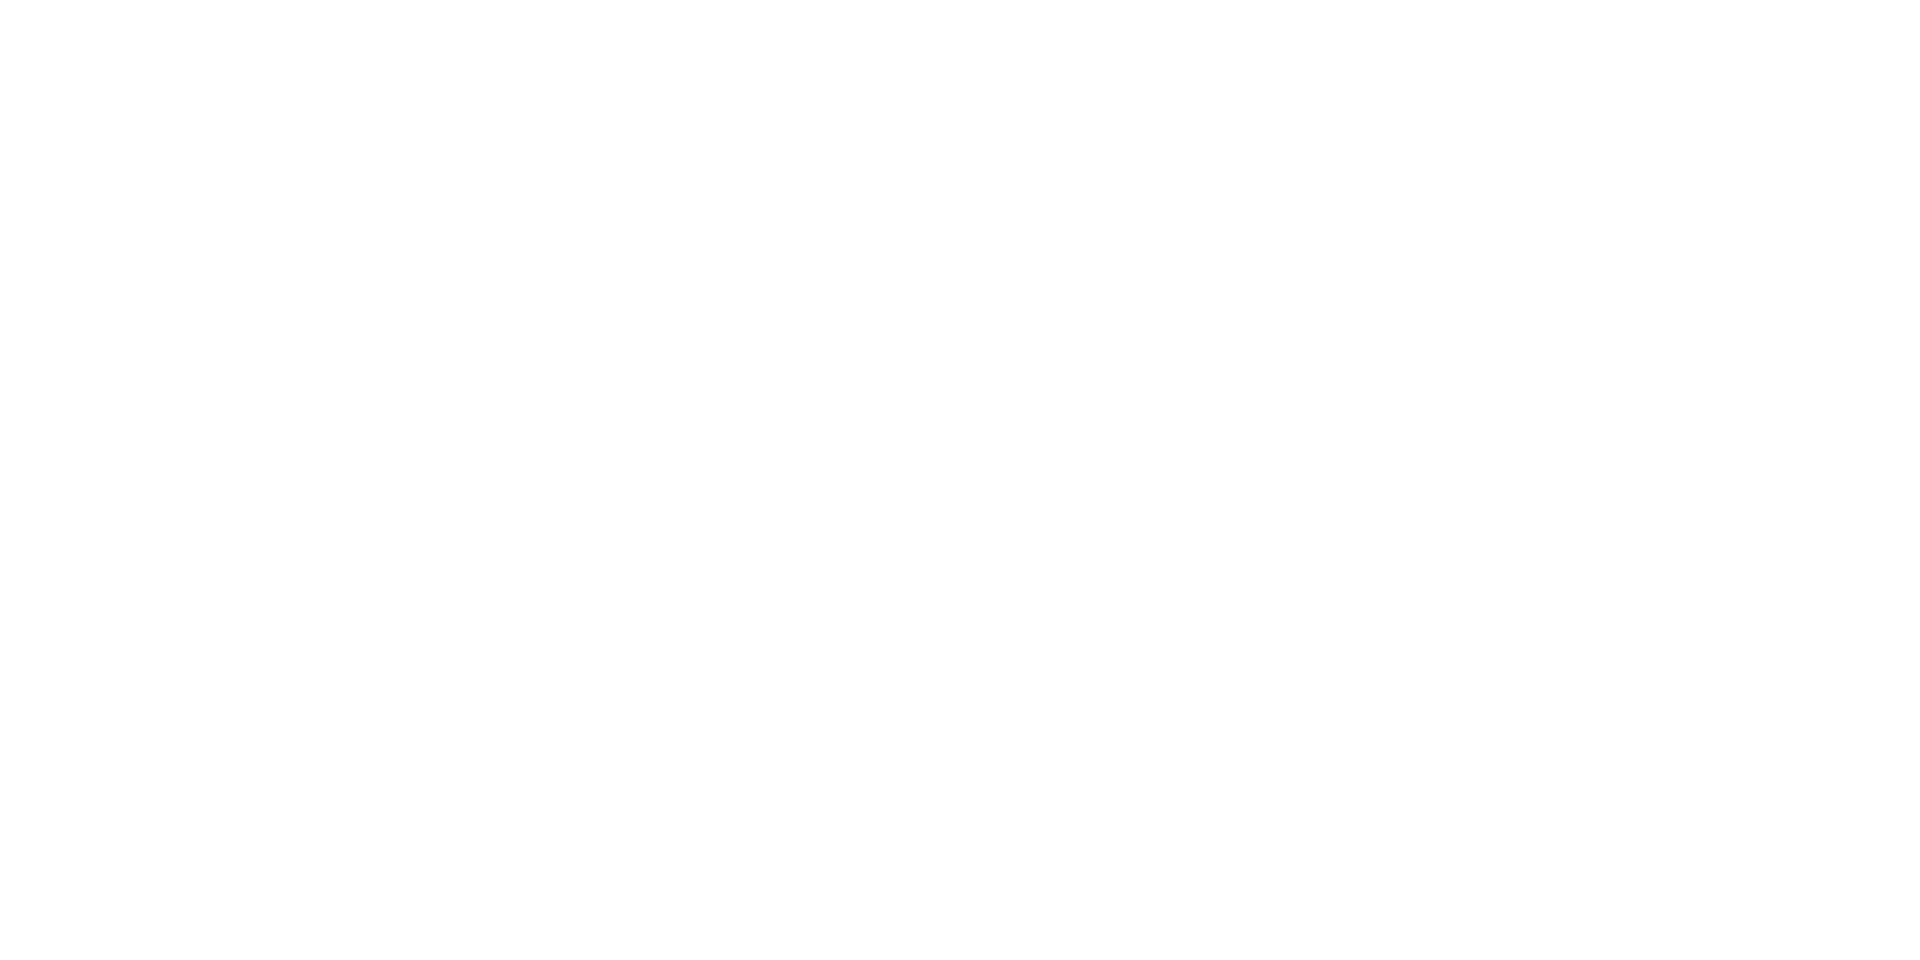
\includegraphics[width=1\linewidth]{figure/NSbox5-1} \end{center}

\hypertarget{fractional-number-conversion-repeated-multiplication-by-2}{%
\paragraph{Fractional number conversion: Repeated multiplication by 2}\label{fractional-number-conversion-repeated-multiplication-by-2}}

\begin{itemize}
\tightlist
\item
  Multiply any factional part repeatedly by 2.
\item
  The equivalent binary number is formed from the 1 or 0 in the units position (\(10^0\) position).
\end{itemize}

\textbf{Example 1: Convert the decimal number 0.625 to binary}

\begin{center}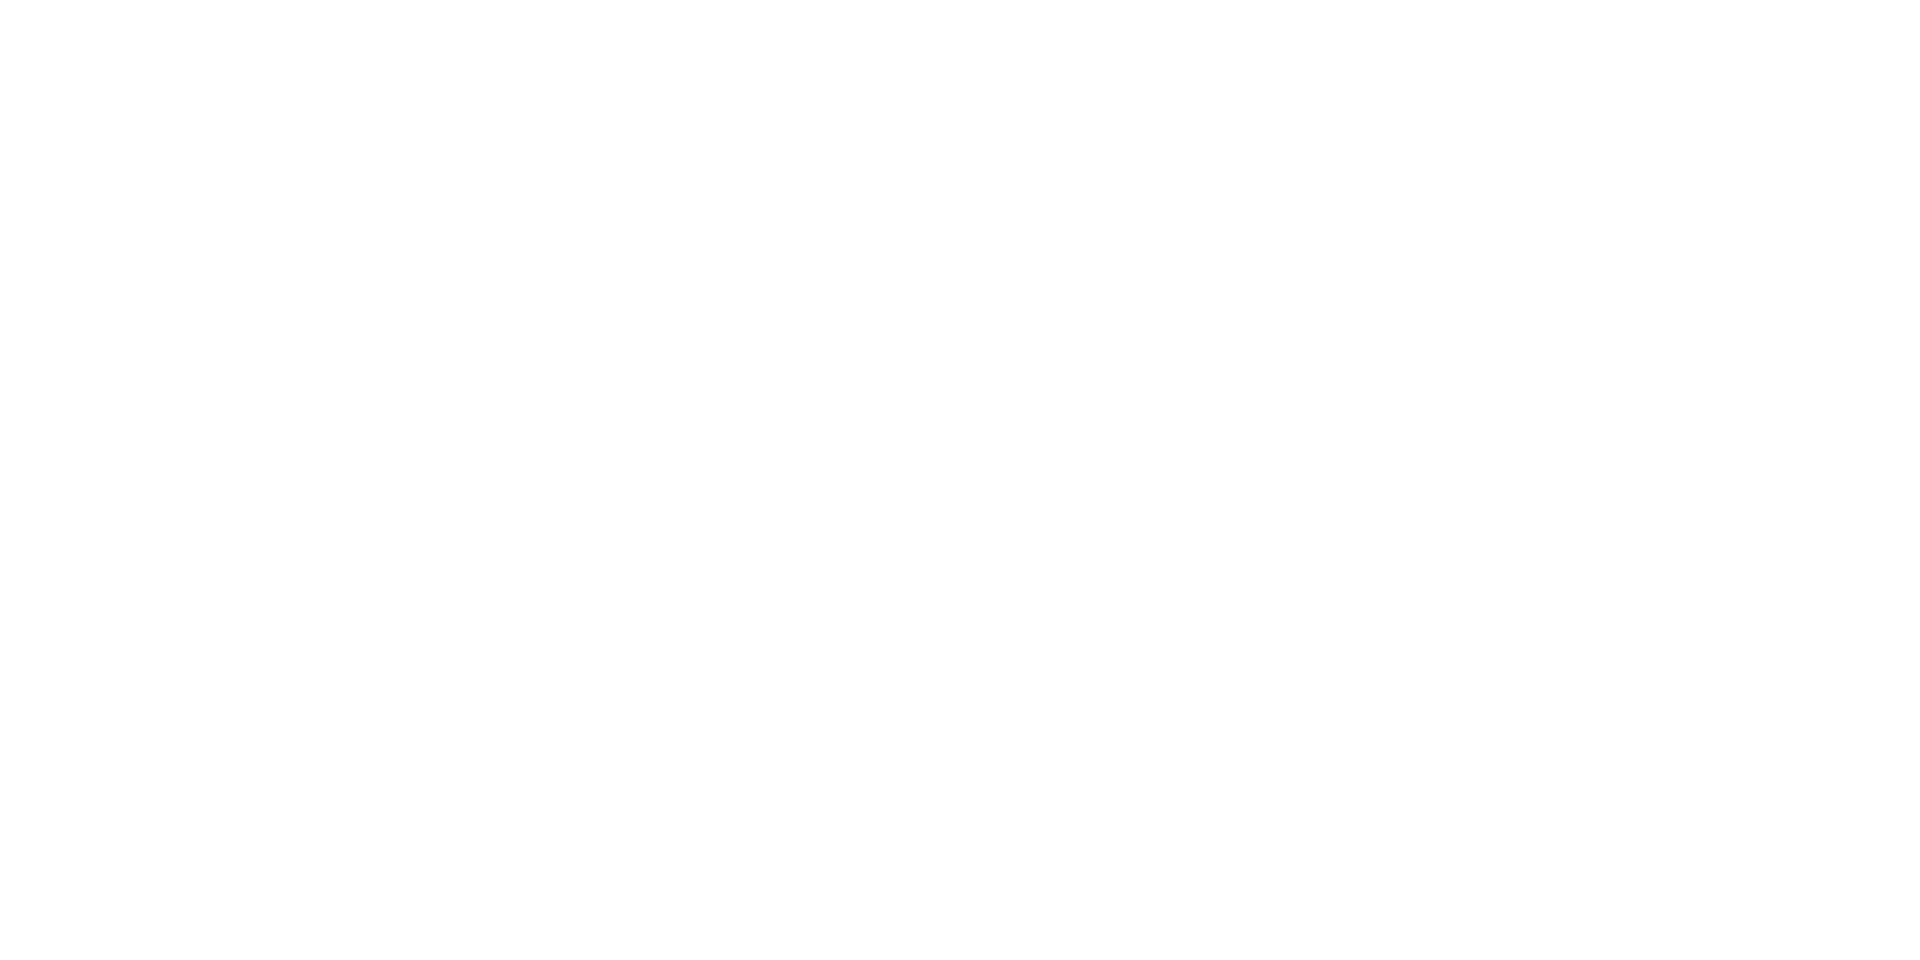
\includegraphics[width=1\linewidth]{figure/NSbox6-1} \end{center}

\begin{itemize}
\tightlist
\item
  Sometimes it will be necessary to terminate the multiplication when an acceptable degree of accuracy is obtained. Then the resulted binary number will be an approximation.
\end{itemize}

\textbf{Example 2: Convert the decimal number 0.6375 to binary}

\begin{center}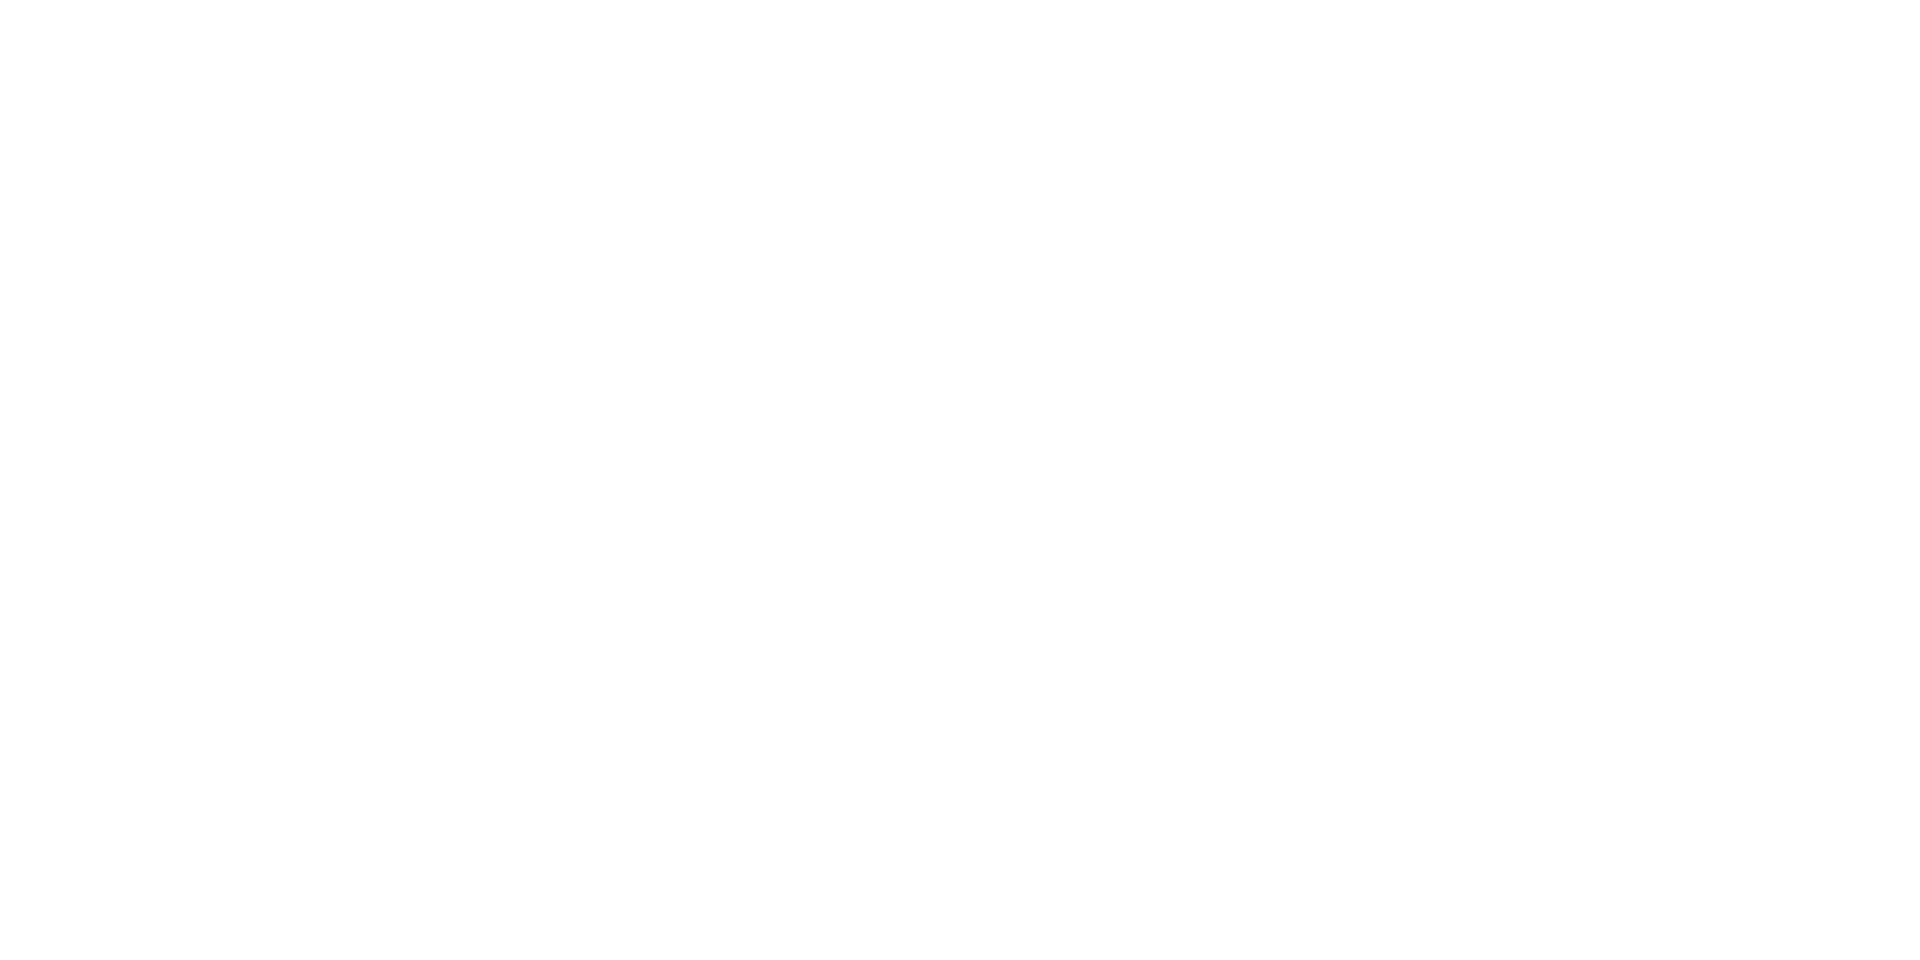
\includegraphics[width=1\linewidth]{figure/NSbox7-1} \end{center}

\begin{itemize}
\item
  We see that it continues in this way and does not terminate.
\item
  So, \(0.6375_{10} = (0.1010001101....)_{2}\).
\item
  If we discard all the bits after the 7th bit, then we get the approximate representation \(0.6375_{10} \approx (0.1010001)_{2},\) committing an error amounting to
  \[0.6375_{10} -(0.1010001)_{2}= 0.6375_{10} -0.6328125_{10}= (.0046875)_{10},\]
  which is known as \textbf{\emph{round-off error}}.
\item
  Although, strictly, this is \emph{chopping-off error}, it is generally, termed as \emph{round-off error}.
\end{itemize}

\textbf{Example 3: Convert the decimal number 49.683 to binary}

\begin{center}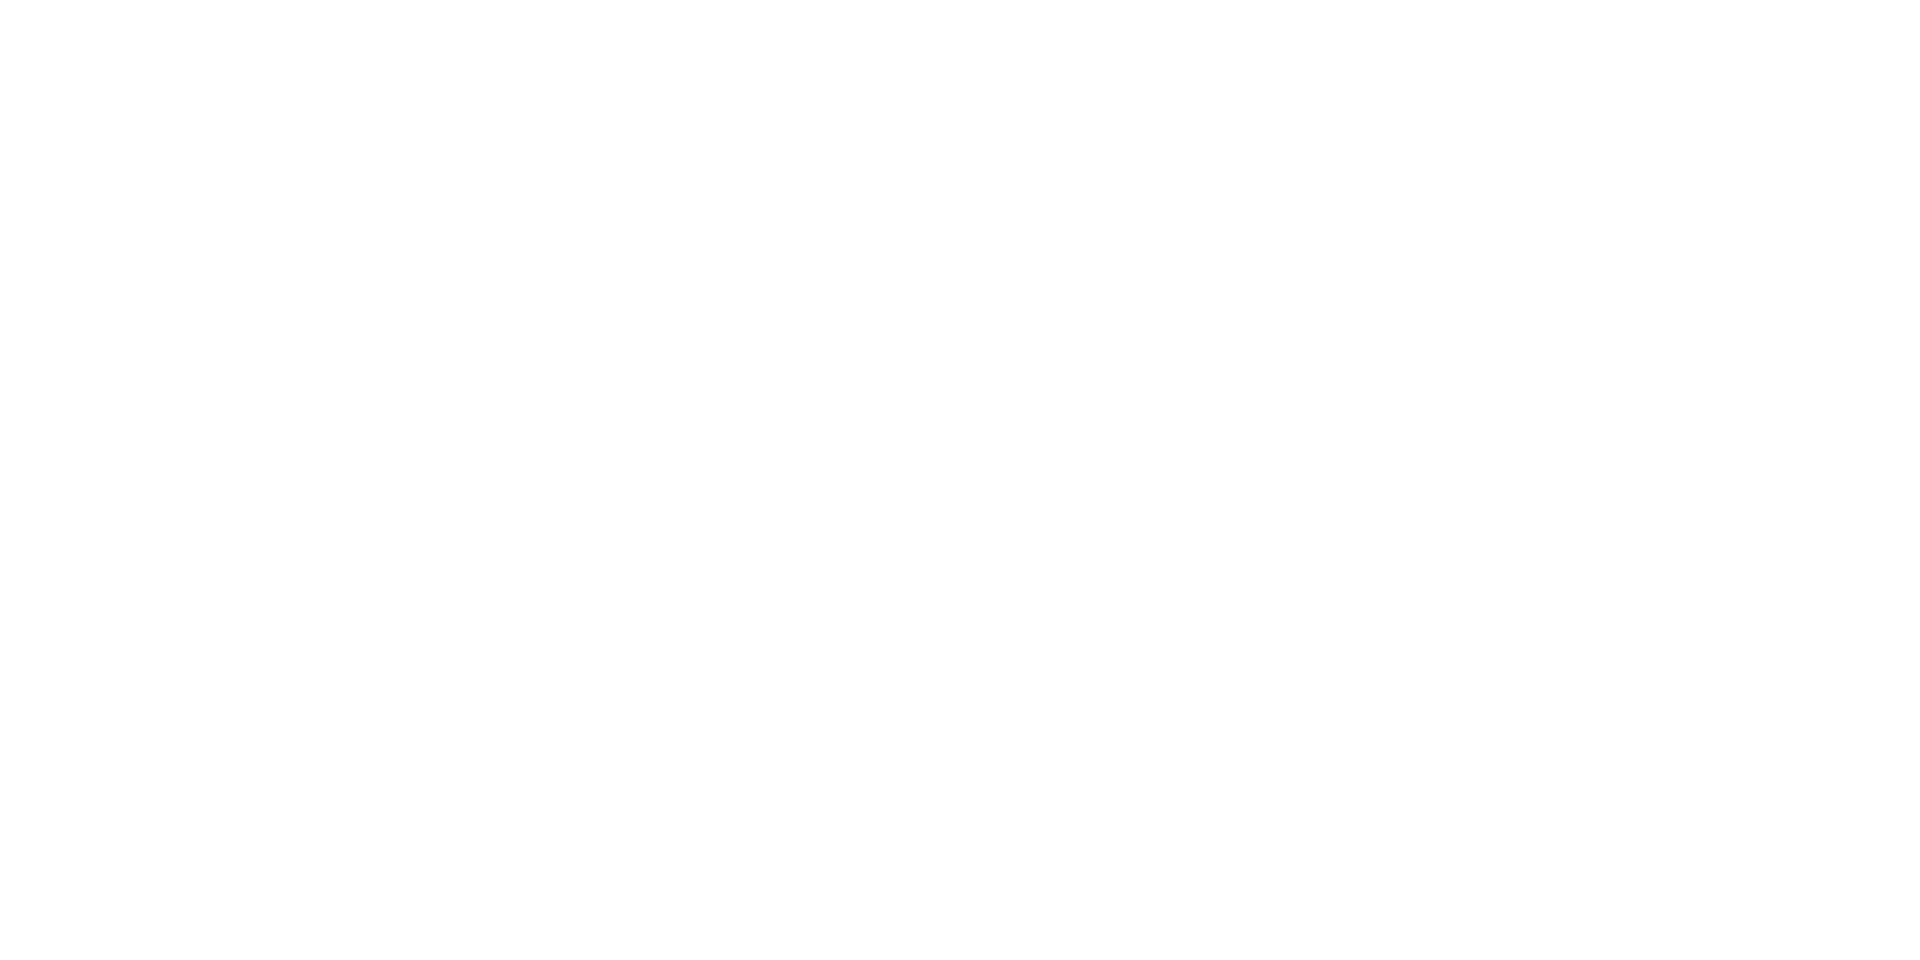
\includegraphics[width=1\linewidth]{figure/NSbox8-1} \end{center}

\hypertarget{octal-number-system}{%
\subsection{Octal Number System}\label{octal-number-system}}

\begin{itemize}
\tightlist
\item
  The octal system is a number system of base or radix equal to 8.
\end{itemize}

\hypertarget{octal-to-decimal-conversion}{%
\subsubsection{Octal-to-Decimal Conversion}\label{octal-to-decimal-conversion}}

\textbf{Example 1: Convert the following octal numbers to their decimal equivalent}

\begin{enumerate}
\def\labelenumi{(\alph{enumi})}
\tightlist
\item
  \(35_8\)
\item
  \(100_8\)
\item
  \(0.24_8\)
\end{enumerate}

\begin{center}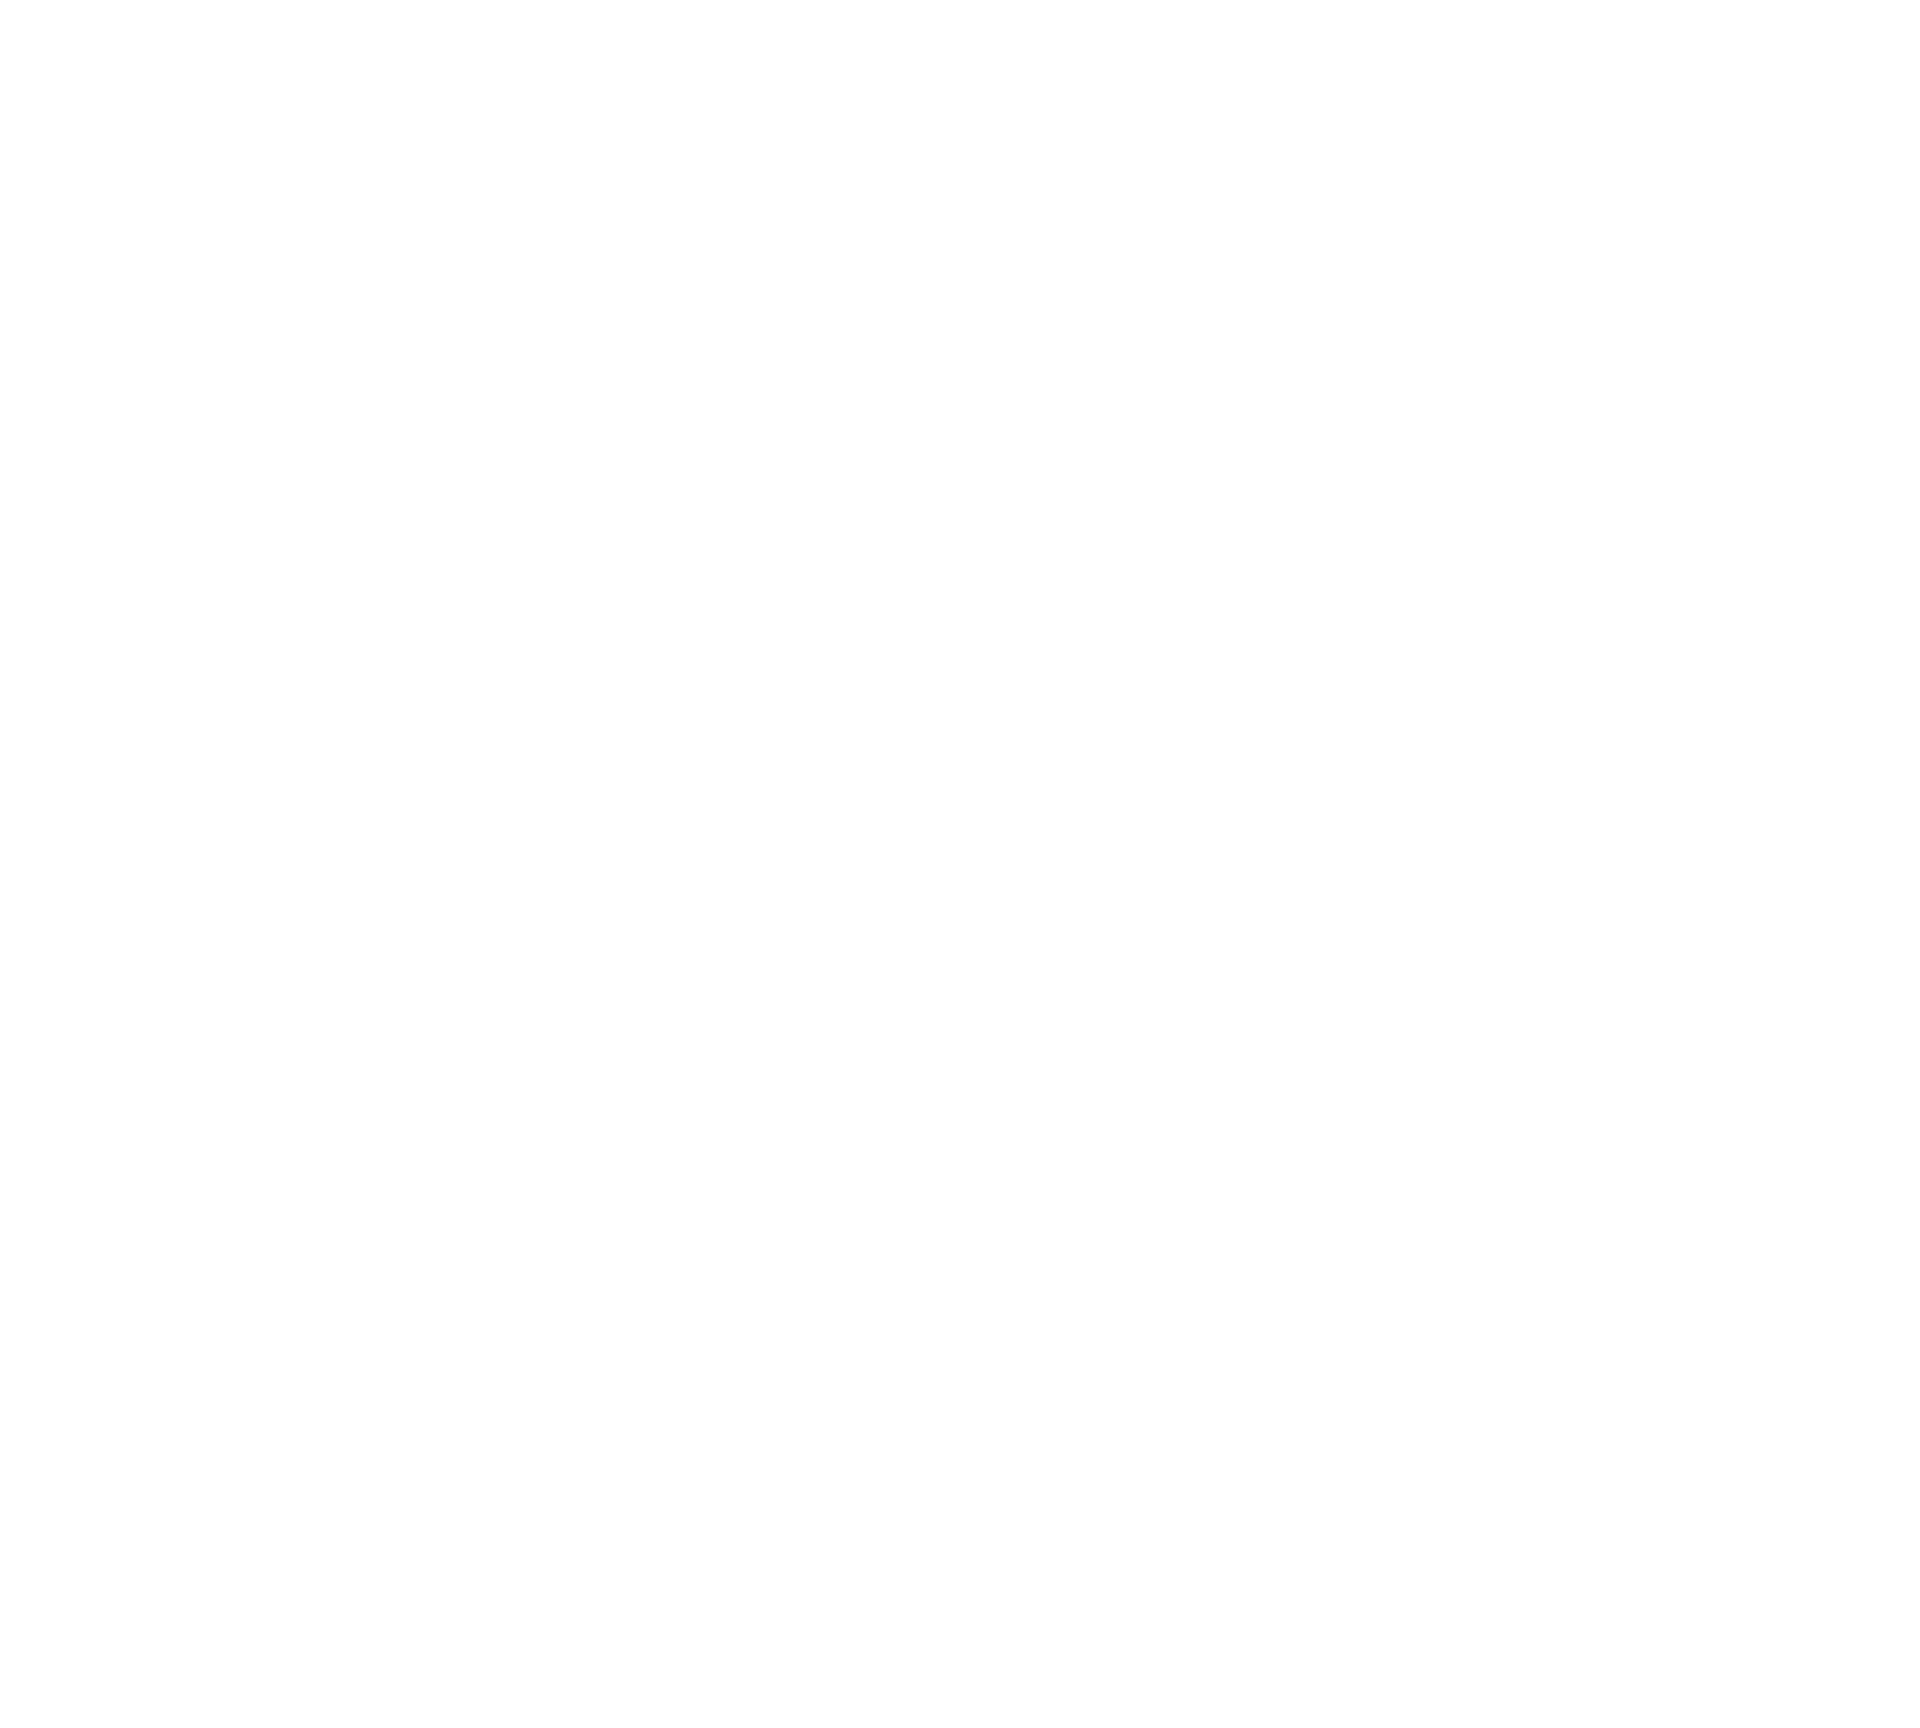
\includegraphics[width=1\linewidth]{figure/NSbox9-1} \end{center}

\hypertarget{decimal-to-octal-conversion}{%
\subsubsection{Decimal-to-Octal Conversion}\label{decimal-to-octal-conversion}}

\begin{itemize}
\tightlist
\item
  To convert decimal numbers to their octal equivalent, the following procedures are employed:
\end{itemize}

\hypertarget{whole-number-conversion-repeated-division-by-8}{%
\paragraph{Whole number conversion: Repeated division by 8}\label{whole-number-conversion-repeated-division-by-8}}

\textbf{Example 1: Convert the decimal number 245 to octal equivalent}

\begin{center}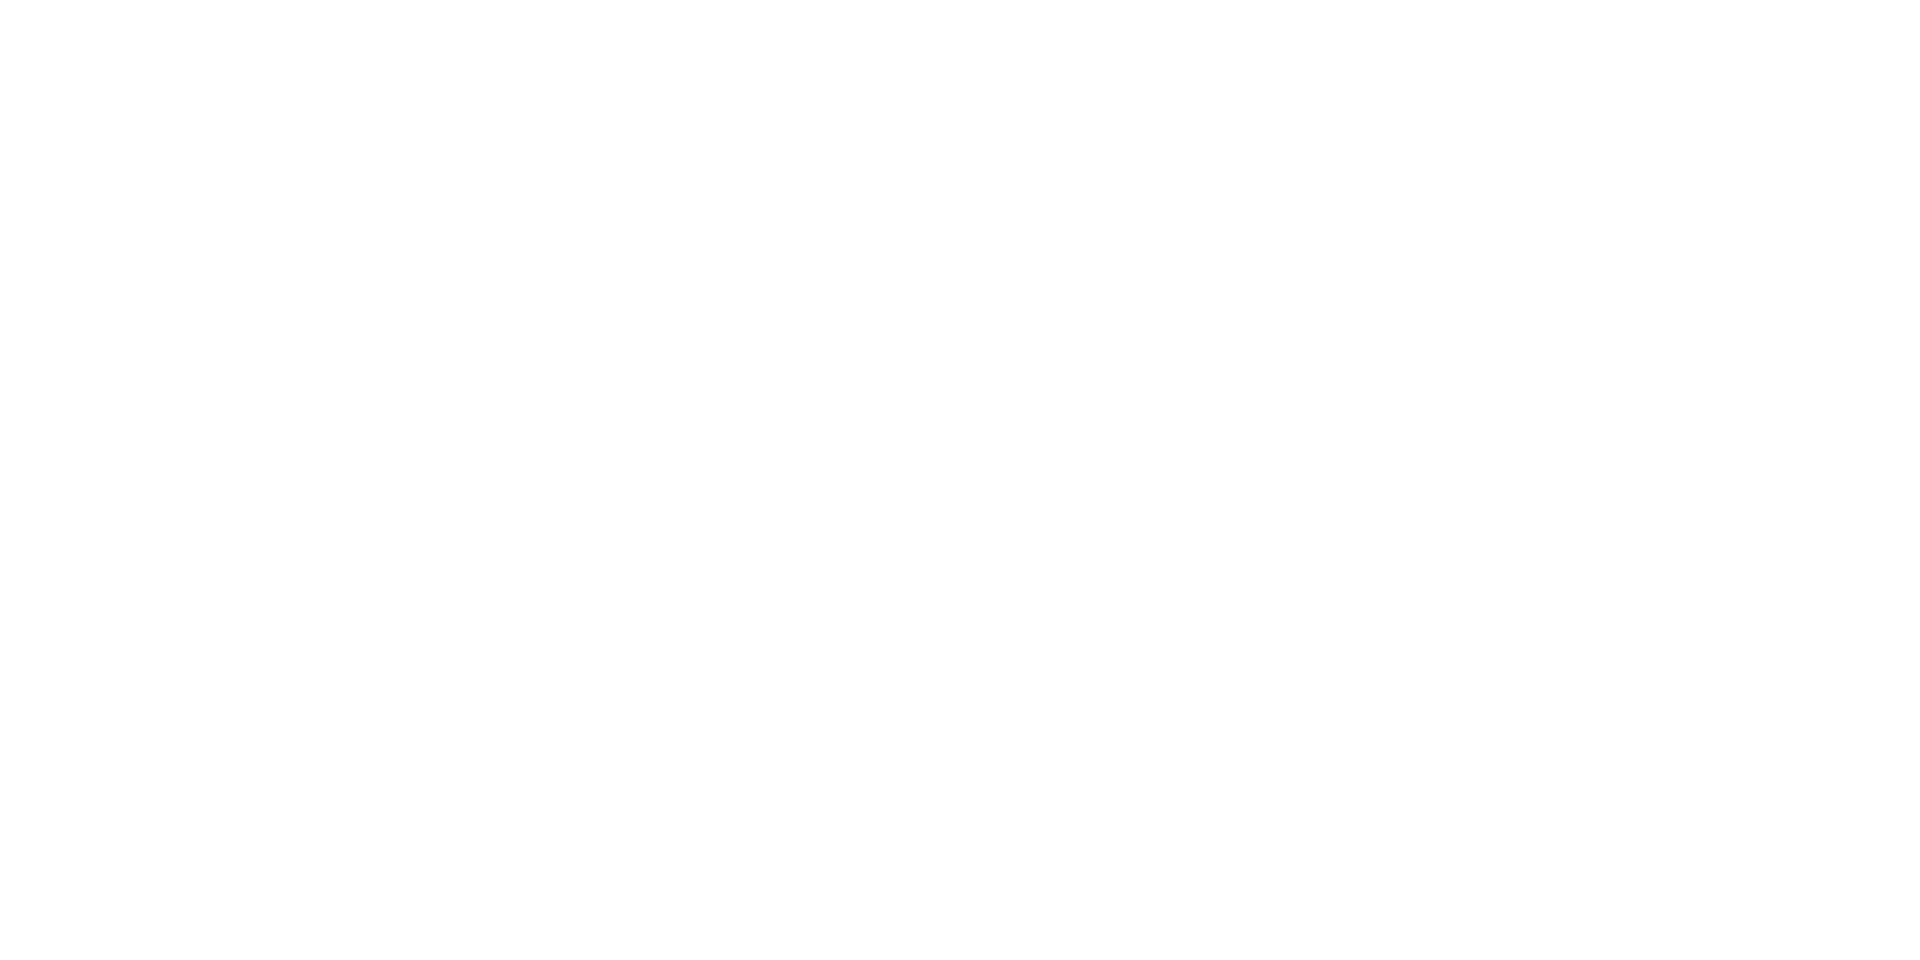
\includegraphics[width=1\linewidth]{figure/NSbox10-1} \end{center}

\hypertarget{fractional-number-conversion-repeated-multiplication-by-8}{%
\paragraph{Fractional number conversion: Repeated multiplication by 8}\label{fractional-number-conversion-repeated-multiplication-by-8}}

\textbf{Example 2: Convert the decimal fraction 0.432 to octal equivalent}

\begin{center}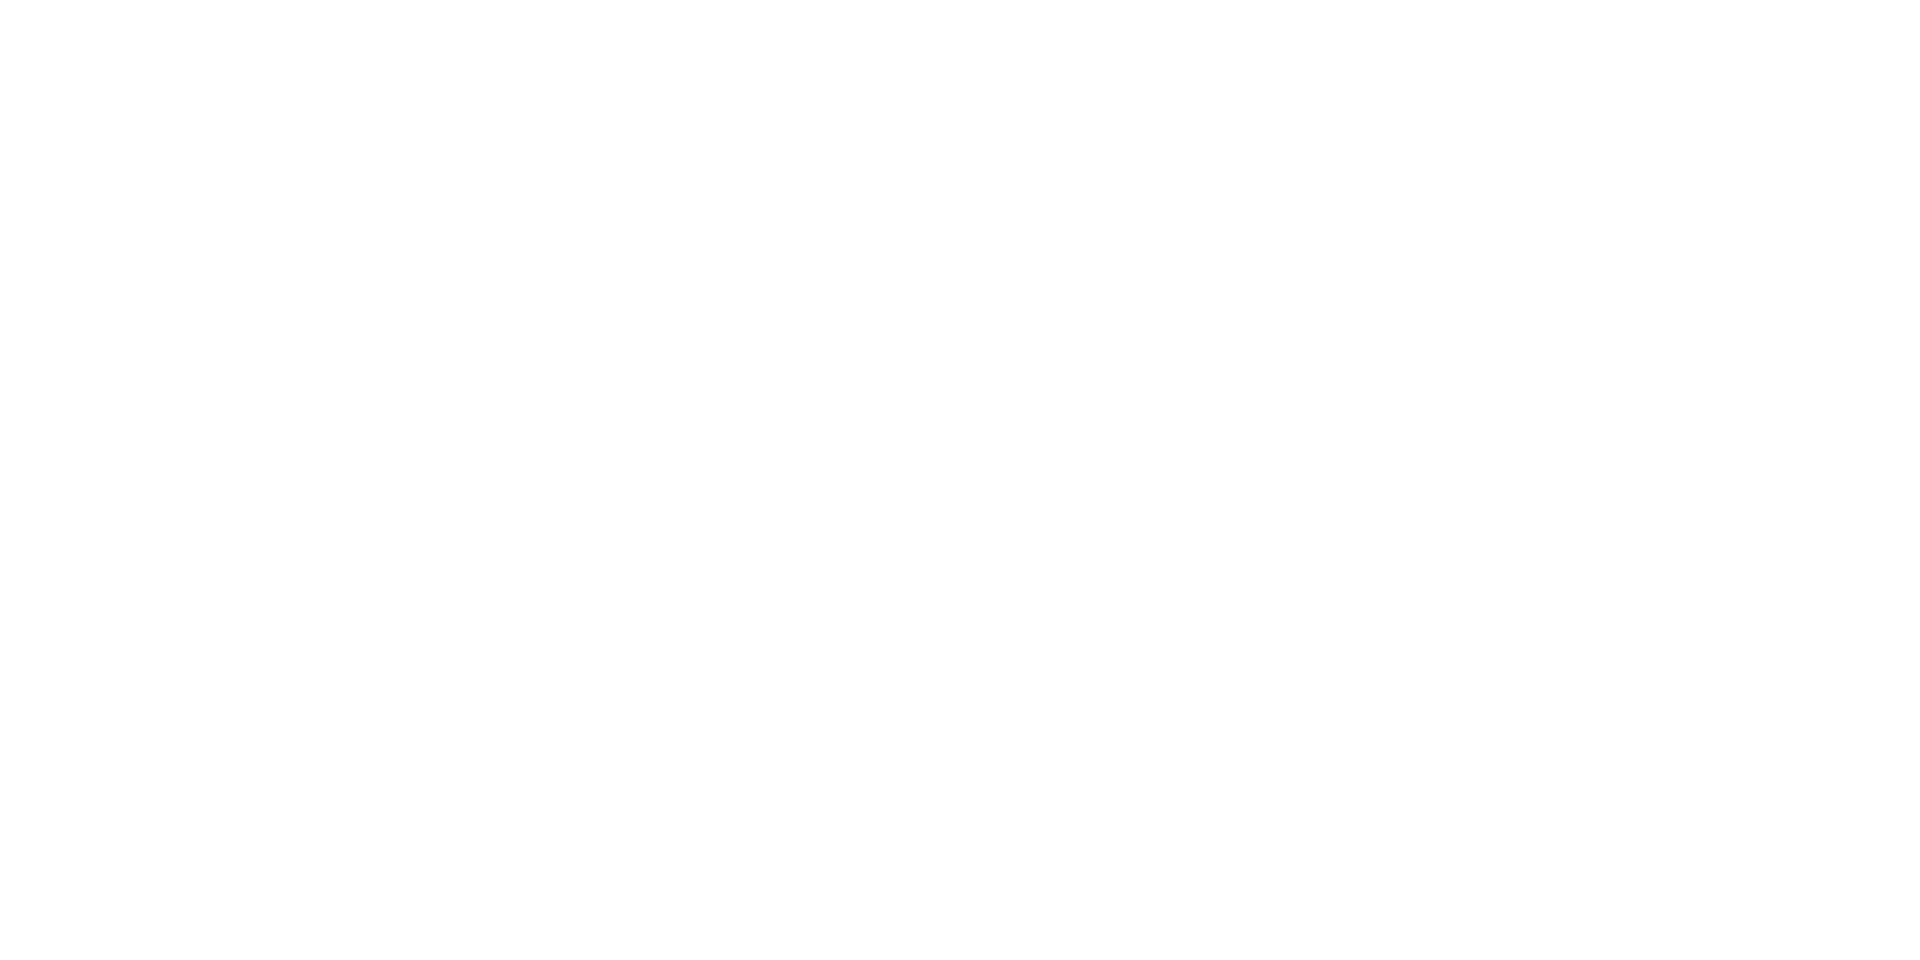
\includegraphics[width=1\linewidth]{figure/NSbox11-1} \end{center}

\begin{itemize}
\tightlist
\item
  This conversion to octal is not precise as there is a remainder.
\item
  If greater accuracy is required, continue multiplying by 8 to obtain more octal digits.
\end{itemize}

\textbf{Example 3: Convert the decimal number 419.95 to octal equivalent}

\begin{center}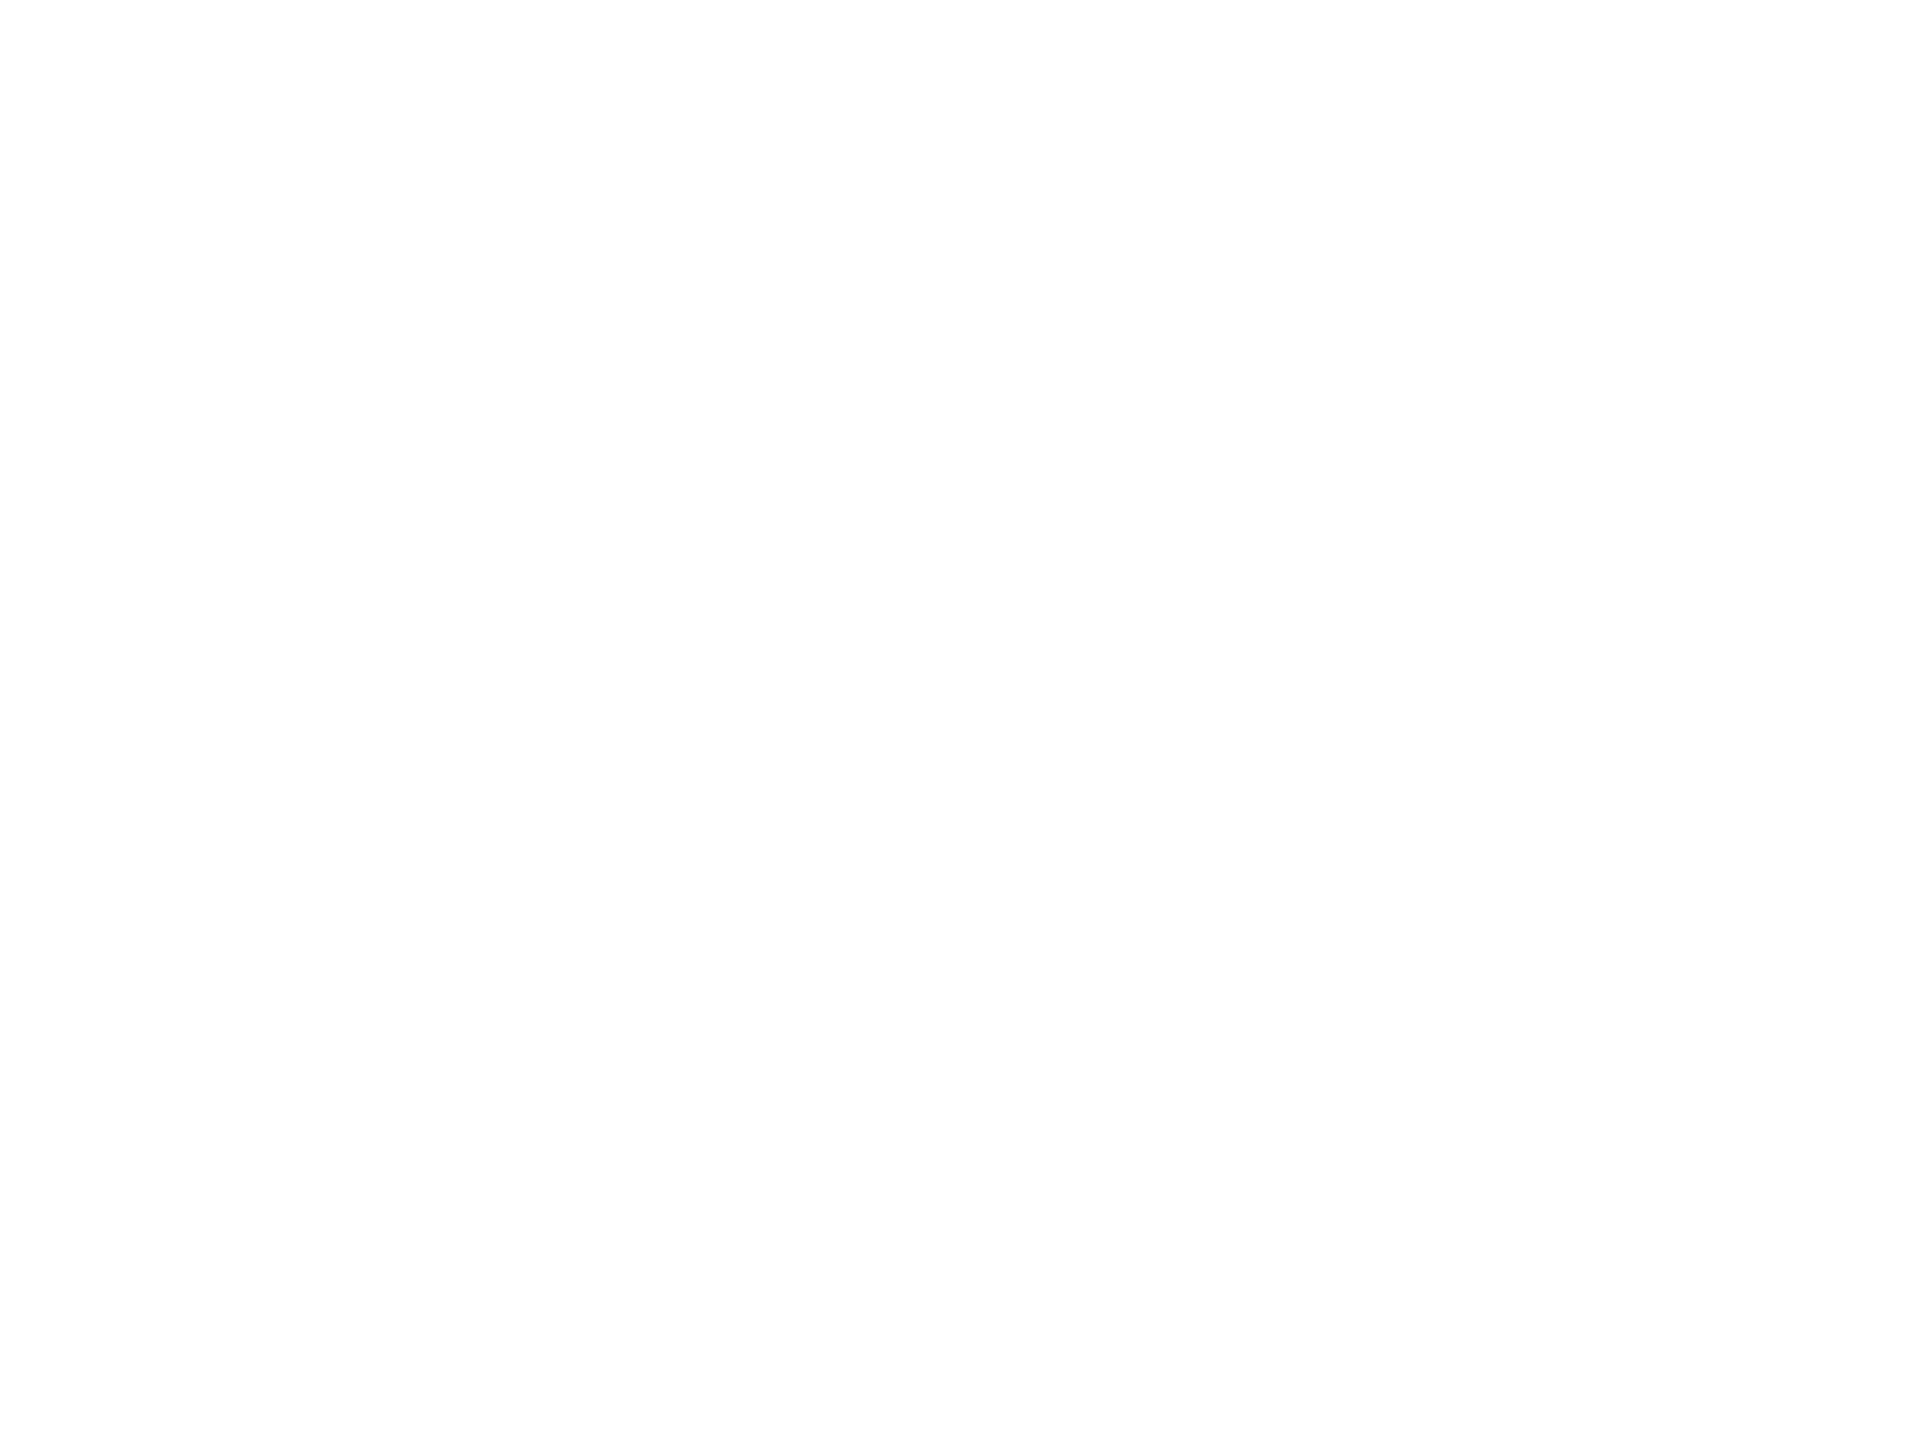
\includegraphics[width=1\linewidth]{figure/NSbox12-1} \end{center}

\hypertarget{octal-to-binary-conversion}{%
\subsubsection{Octal-to-Binary Conversion}\label{octal-to-binary-conversion}}

\textbf{Octal and binary number correspondence}

\begin{longtable}[]{@{}ll@{}}
\toprule
Octal & Binary\tabularnewline
\midrule
\endhead
0 & 000\tabularnewline
1 & 001\tabularnewline
2 & 010\tabularnewline
3 & 011\tabularnewline
4 & 100\tabularnewline
5 & 101\tabularnewline
6 & 110\tabularnewline
7 & 111\tabularnewline
\bottomrule
\end{longtable}

\begin{itemize}
\tightlist
\item
  To convert from octal to binary, simply replace each octal digit with the corresponding three-digit binary number.
\end{itemize}

\textbf{Example 1: Convert the following octal numbers to their binary equivalent}

\begin{enumerate}
\def\labelenumi{(\alph{enumi})}
\tightlist
\item
  \(247_8\)
\item
  \(124.375_8\)
\end{enumerate}

\begin{center}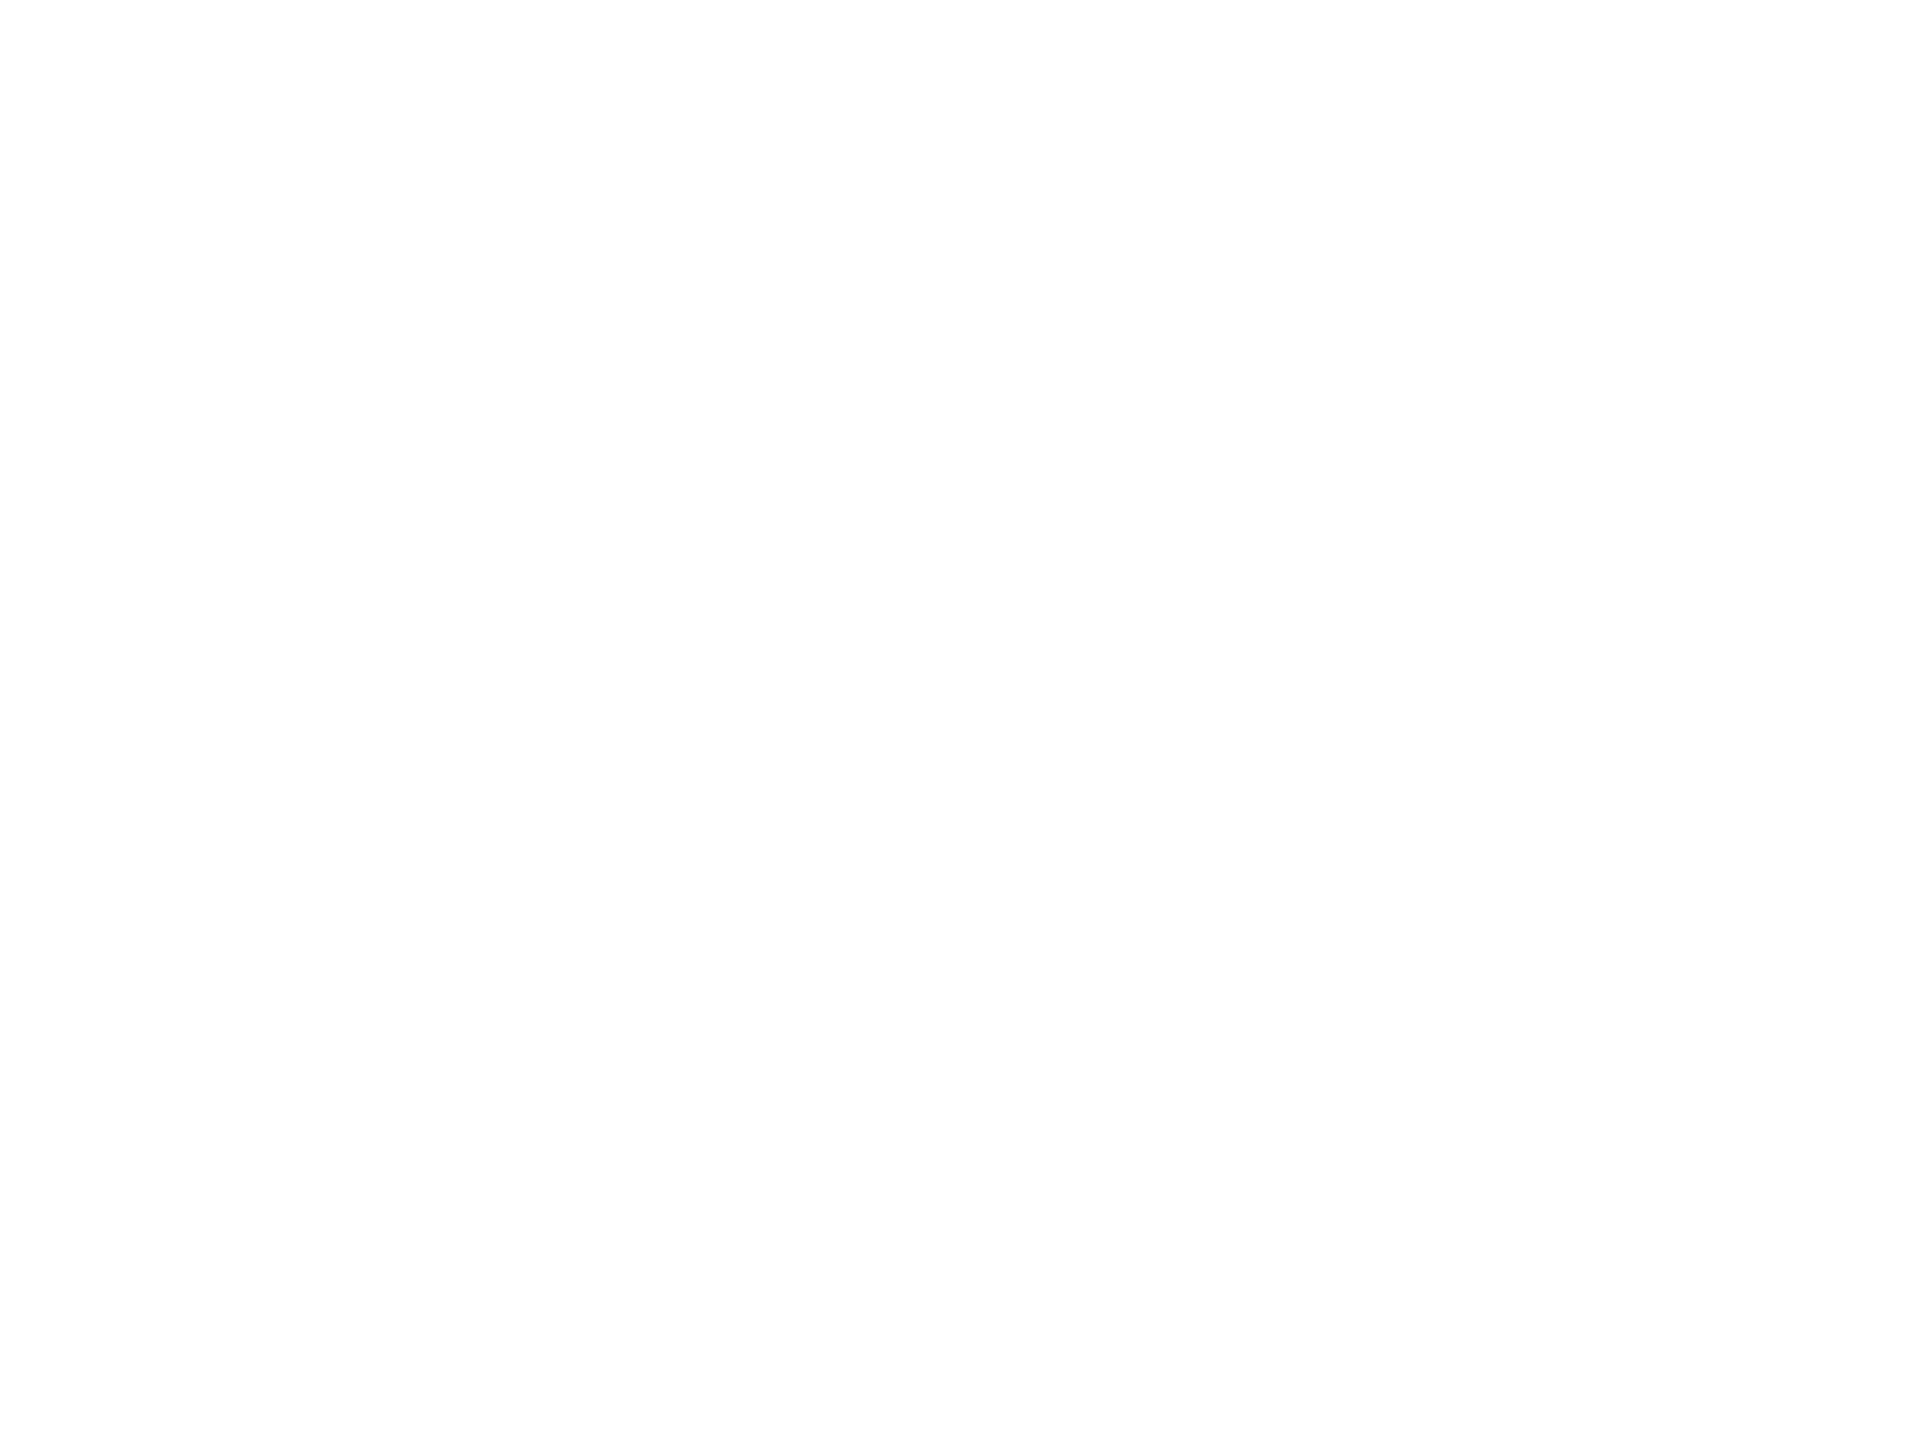
\includegraphics[width=1\linewidth]{figure/NSbox131-1} \end{center}

\hypertarget{binary-to-octal-conversion}{%
\subsubsection{Binary-to-Octal Conversion}\label{binary-to-octal-conversion}}

\begin{itemize}
\tightlist
\item
  To convert from binary to octal, subdivide the number into groups of three bits, proceeding both left and right from the binary point, and if necessary padding the last group with zero. The octal representation of each group gives the required octal number.
\end{itemize}

\textbf{Example 1: Convert the binary number 11010101.01101 to its octal equivalent}

\begin{center}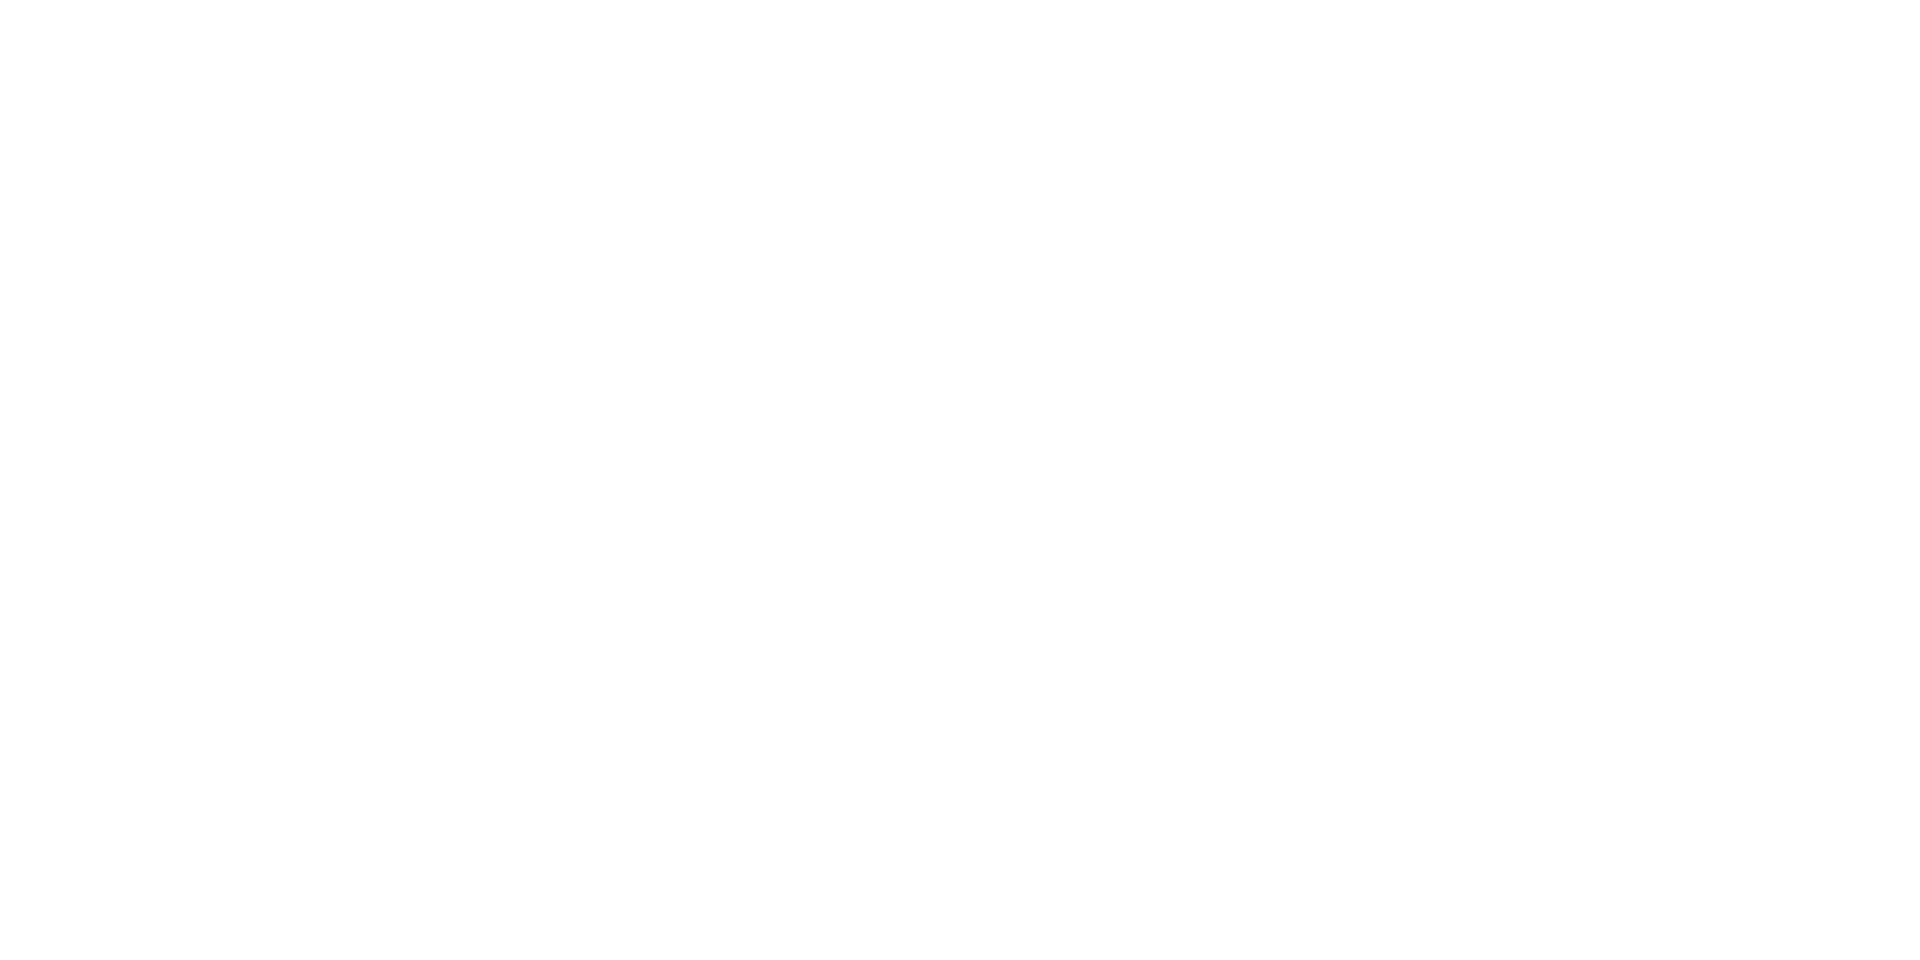
\includegraphics[width=1\linewidth]{figure/NSbox13-1} \end{center}

\hypertarget{hexadecimal-number-system}{%
\subsection{Hexadecimal Number System}\label{hexadecimal-number-system}}

\begin{itemize}
\tightlist
\item
  The Hexadecimal system is a number system of base or radix equal to 16.
\item
  Hexadecimal is similar to the octal numeral system because each can be easily compared to the binary numeral system.
\item
  Example values of hexadecimal numbers converted into binary, octal and decimal.
\end{itemize}

\begin{longtable}[]{@{}llll@{}}
\toprule
Hexadecimal & Binary & Octal & Decimal\tabularnewline
\midrule
\endhead
0 & 0000 & 0 & 0\tabularnewline
1 & 0001 & 1 & 1\tabularnewline
2 & 0010 & 2 & 2\tabularnewline
3 & 0011 & 3 & 3\tabularnewline
4 & 0100 & 4 & 4\tabularnewline
5 & 0101 & 5 & 5\tabularnewline
6 & 0110 & 6 & 6\tabularnewline
7 & 0111 & 7 & 7\tabularnewline
8 & 1000 & 10 & 8\tabularnewline
9 & 1001 & 11 & 9\tabularnewline
A & 1010 & 12 & 10\tabularnewline
B & 1011 & 13 & 11\tabularnewline
C & 1100 & 14 & 12\tabularnewline
D & 1101 & 15 & 13\tabularnewline
E & 1110 & 16 & 14\tabularnewline
F & 1111 & 17 & 15\tabularnewline
\bottomrule
\end{longtable}

\hypertarget{hexadecimal-to-decimal-conversion}{%
\subsubsection{Hexadecimal-to-Decimal Conversion}\label{hexadecimal-to-decimal-conversion}}

\textbf{Example 1: Convert the following octal numbers to their decimal equivalent}

\begin{enumerate}
\def\labelenumi{(\alph{enumi})}
\tightlist
\item
  \(C7_{16}\)
\item
  \(2F_{16}\)
\end{enumerate}

\begin{center}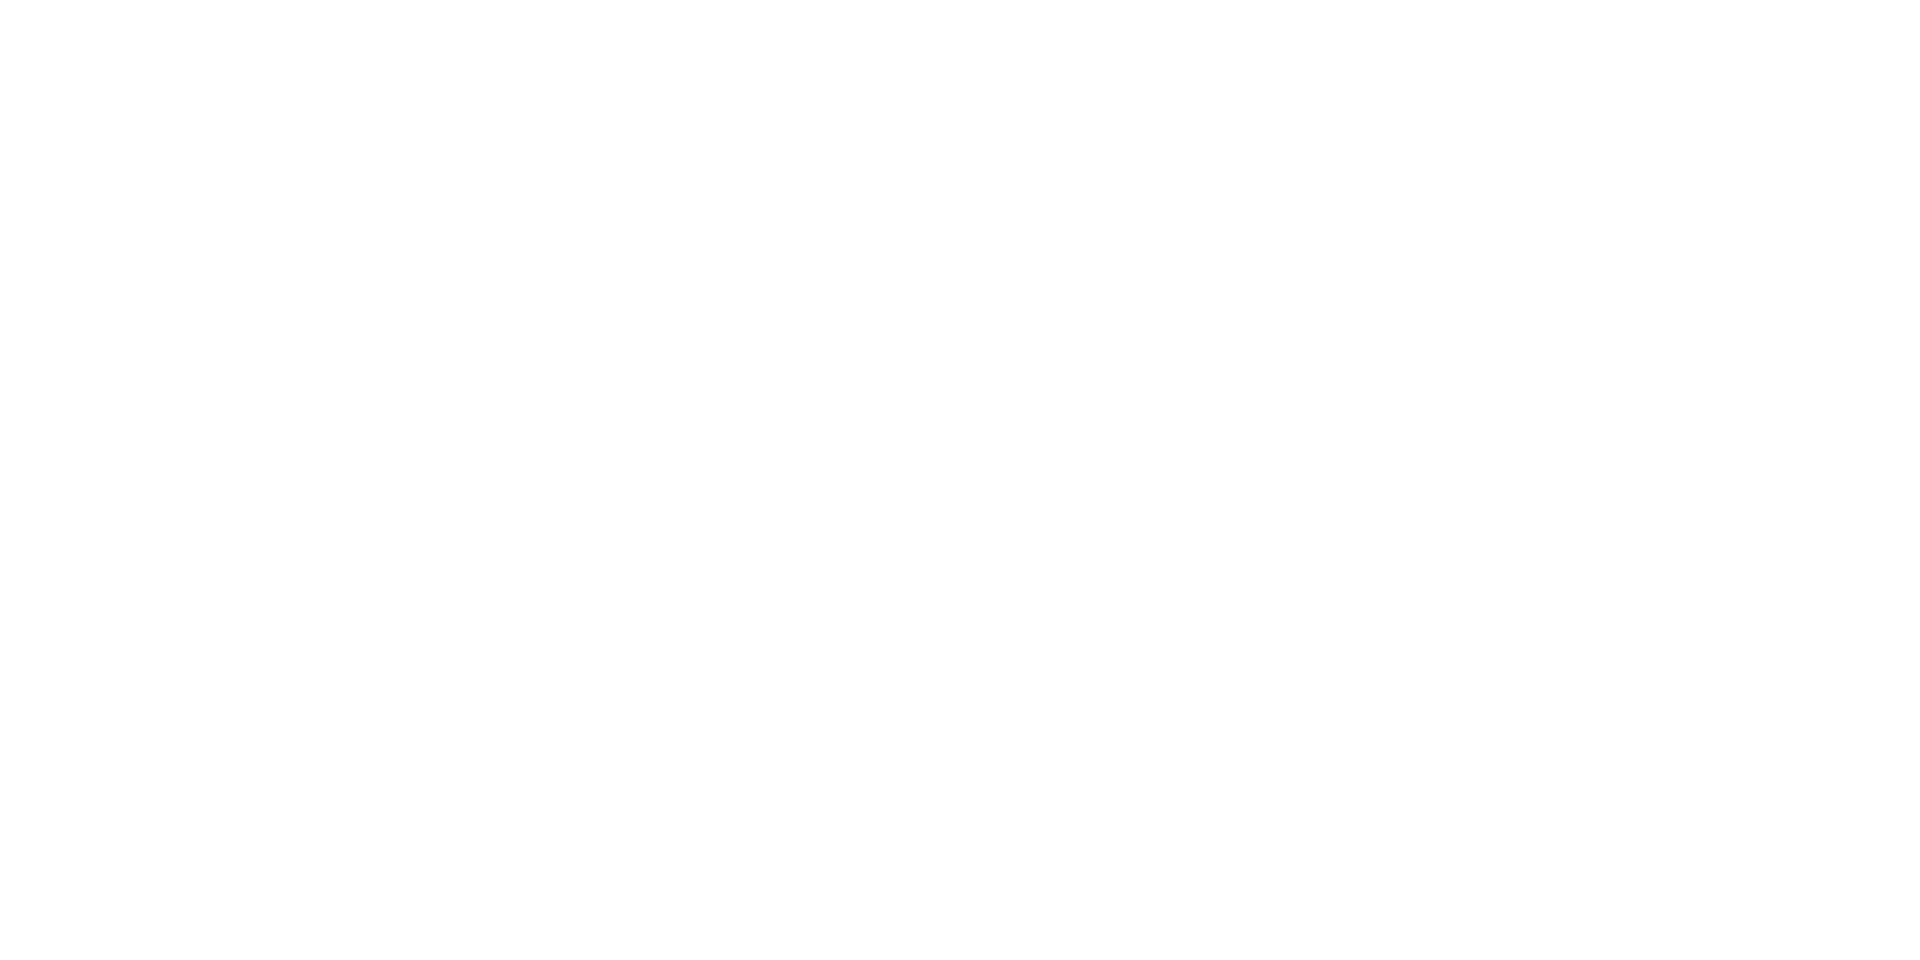
\includegraphics[width=1\linewidth]{figure/NSbox14-1} \end{center}

\hypertarget{decimal-to-hexadecimal-conversion}{%
\subsubsection{Decimal-to-Hexadecimal Conversion}\label{decimal-to-hexadecimal-conversion}}

\begin{itemize}
\tightlist
\item
  To convert decimal numbers to their hexadecimal equivalent, the following procedures are employed:
\end{itemize}

\hypertarget{whole-number-conversion-repeated-division-by-16}{%
\paragraph{Whole number conversion: Repeated division by 16}\label{whole-number-conversion-repeated-division-by-16}}

\textbf{Example 1: Convert the decimal number 245 to Hexadecimal equivalent}

\begin{center}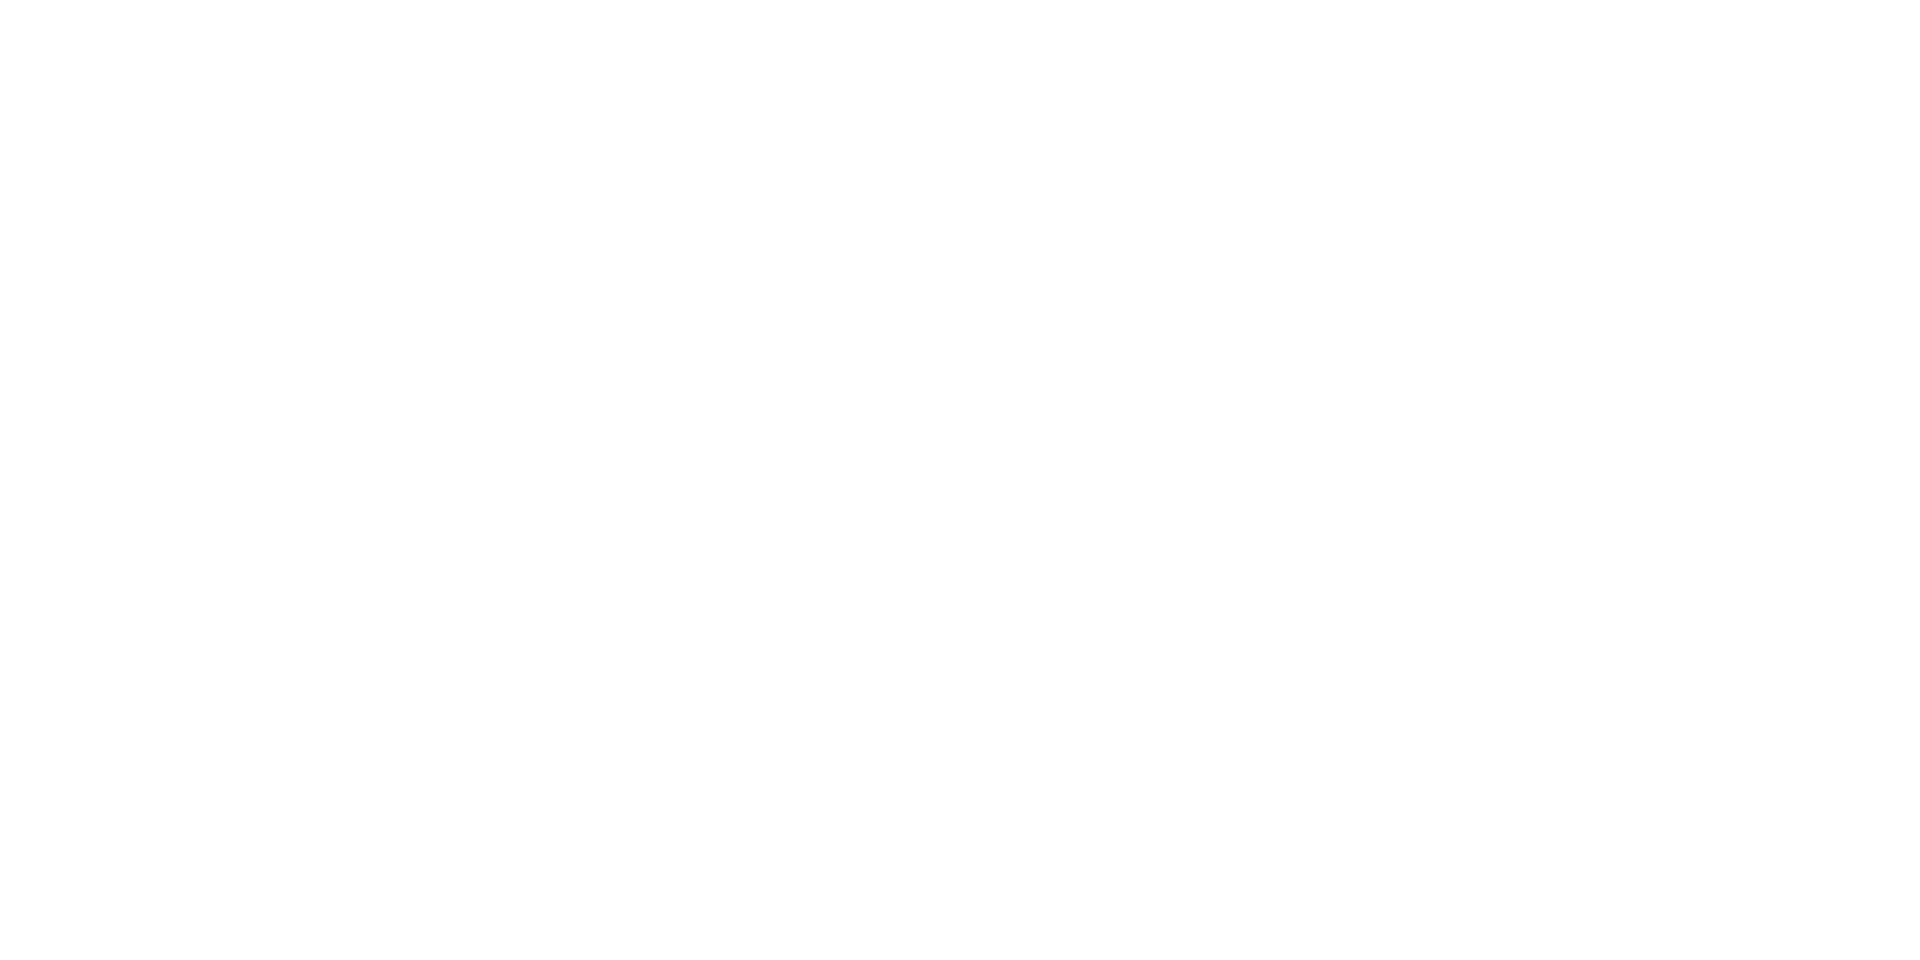
\includegraphics[width=1\linewidth]{figure/NSbox15-1} \end{center}

\hypertarget{fractional-number-conversion-repeated-multiplication-by-16}{%
\paragraph{Fractional number conversion: Repeated multiplication by 16}\label{fractional-number-conversion-repeated-multiplication-by-16}}

\textbf{Example 2: Convert the decimal fraction 0.0738 to Hexadecimal equivalent}

\begin{center}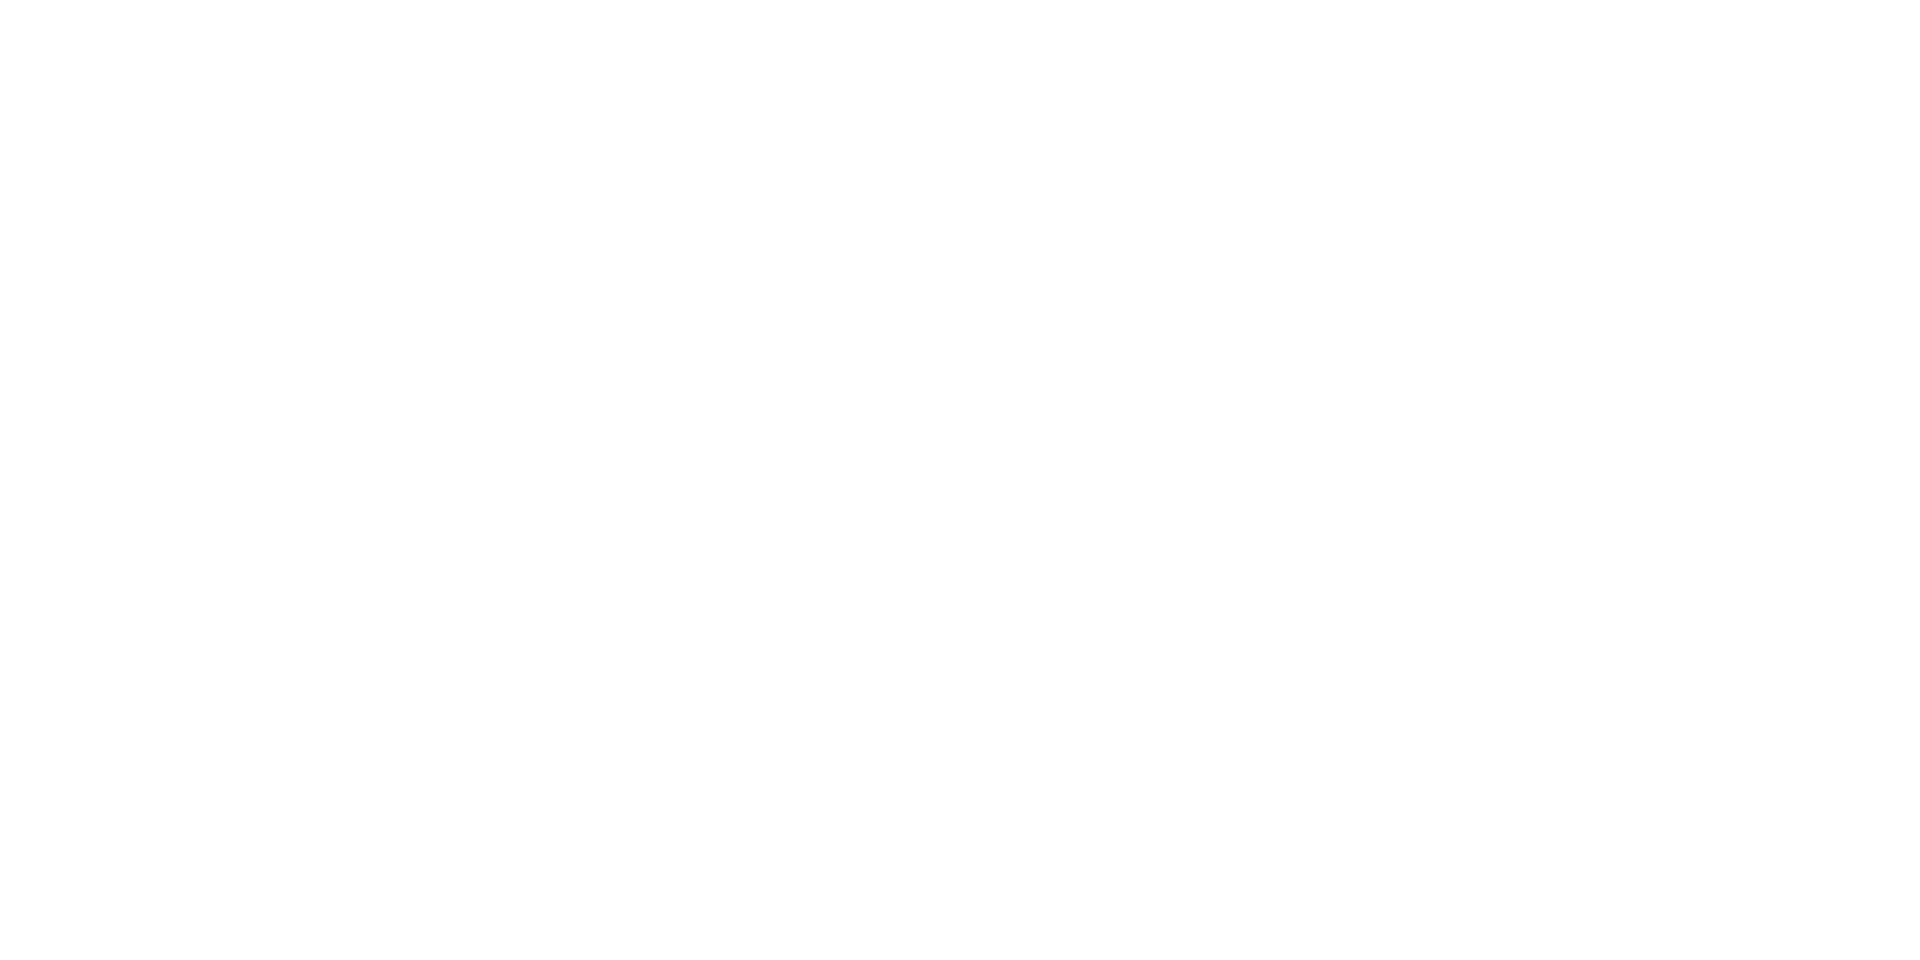
\includegraphics[width=1\linewidth]{figure/NSbox16-1} \end{center}

\textbf{Example 3: Convert the decimal number 420.0095 to Hexadecimal equivalent}

\begin{center}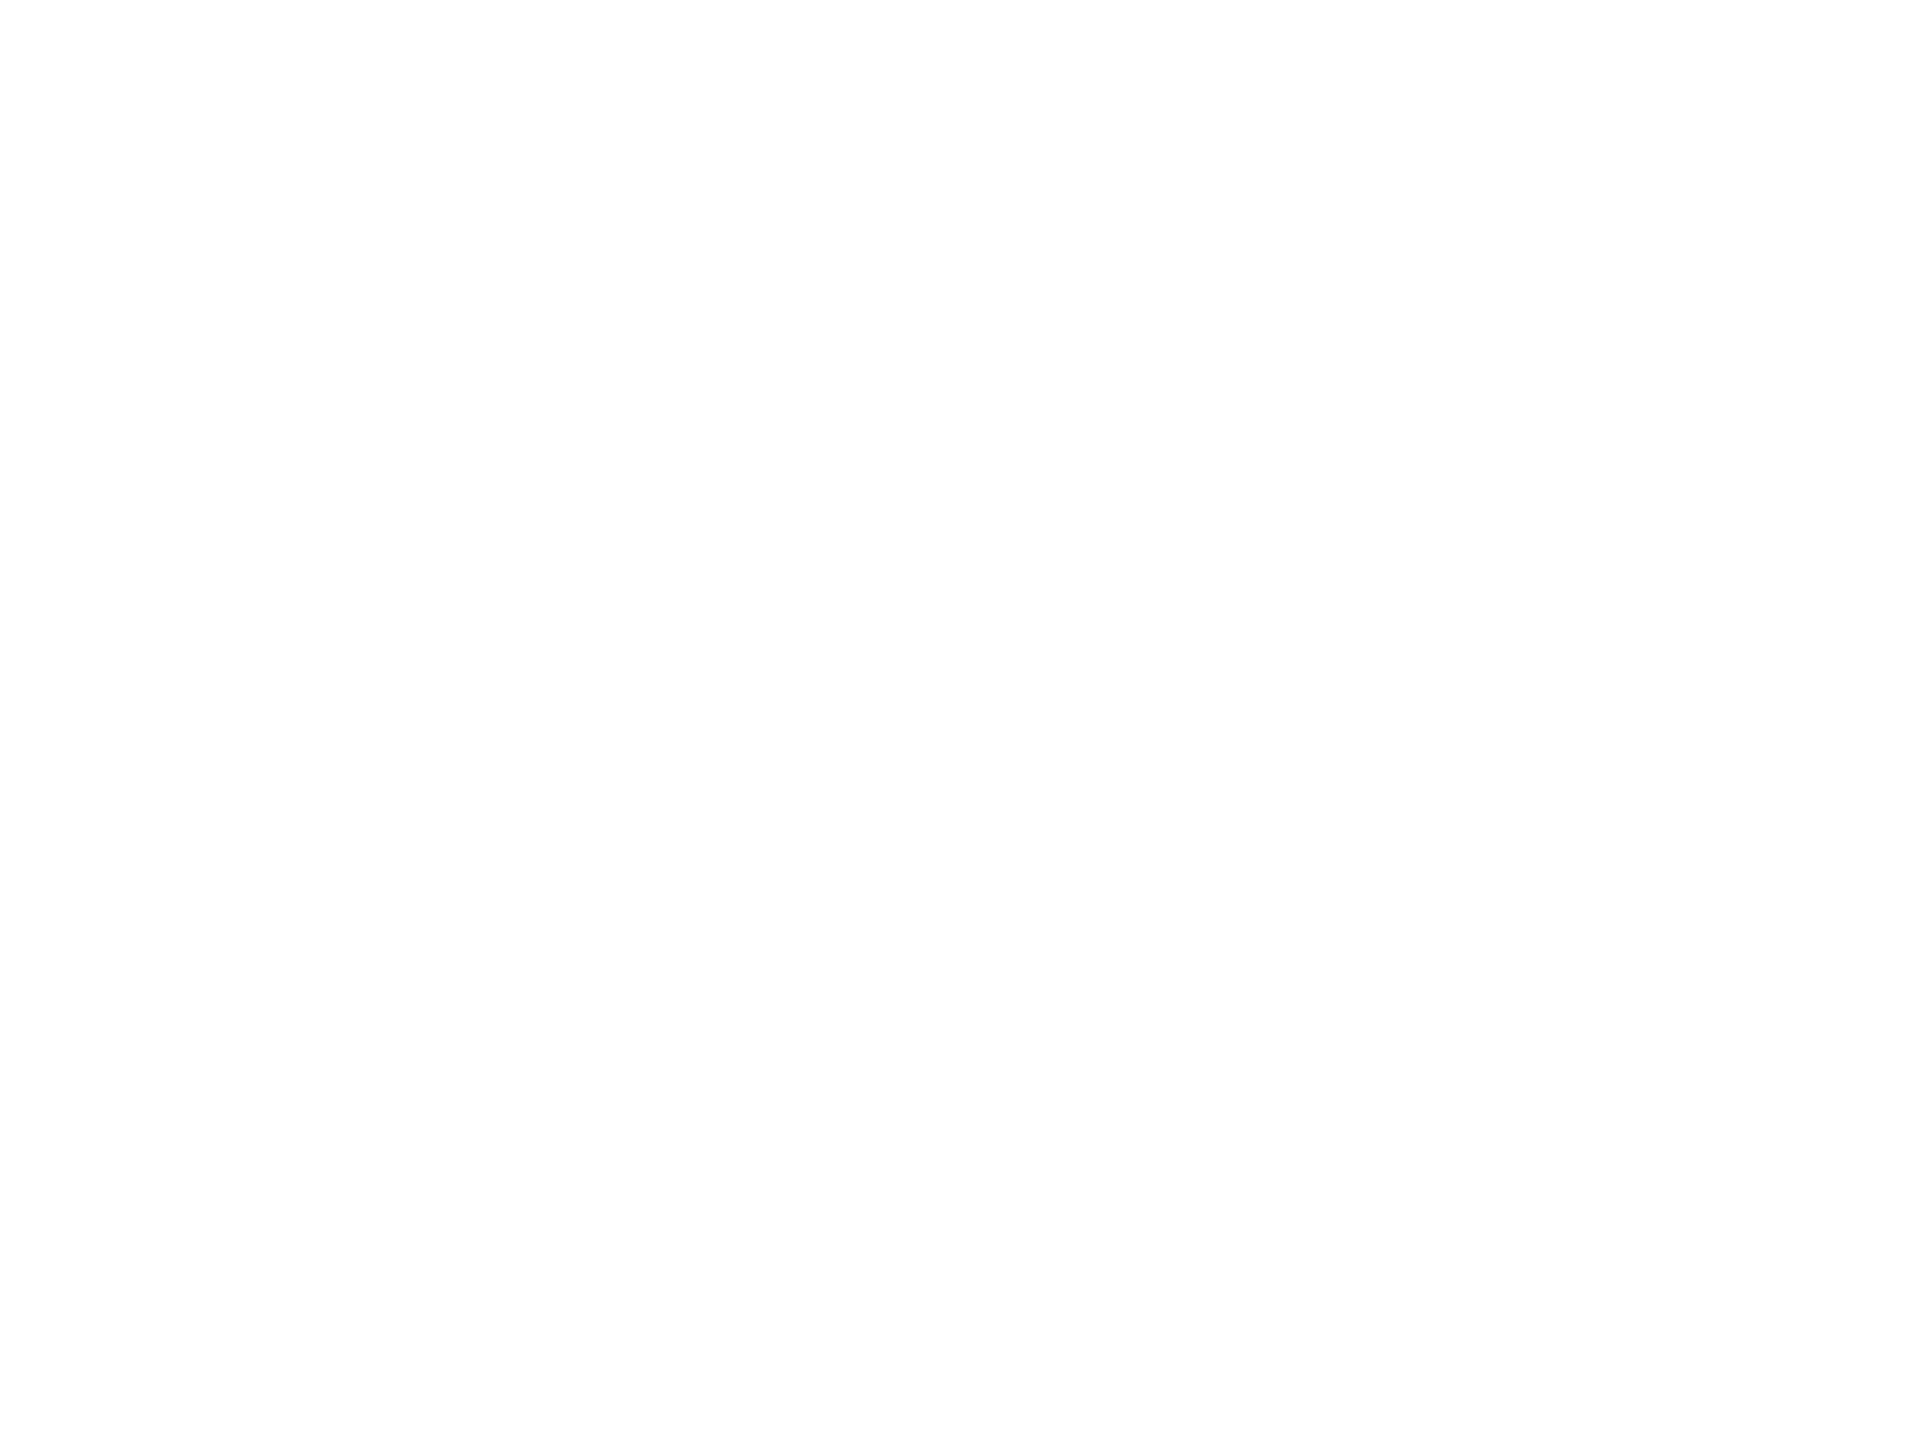
\includegraphics[width=1\linewidth]{figure/NSbox17-1} \end{center}

\hypertarget{hexadecimal-to-binary-conversion}{%
\subsubsection{Hexadecimal-to-Binary Conversion}\label{hexadecimal-to-binary-conversion}}

\begin{itemize}
\tightlist
\item
  To convert from Hexadecimal to binary, simply replace each Hexadecimal digit with the corresponding four-digit binary number.
\end{itemize}

\textbf{Example 1: Convert the following Hexadecimal numbers to their binary equivalent}

\begin{enumerate}
\def\labelenumi{(\alph{enumi})}
\tightlist
\item
  \(7B_{16}\)
\item
  \(6D.8C_{16}\)
\end{enumerate}

\begin{center}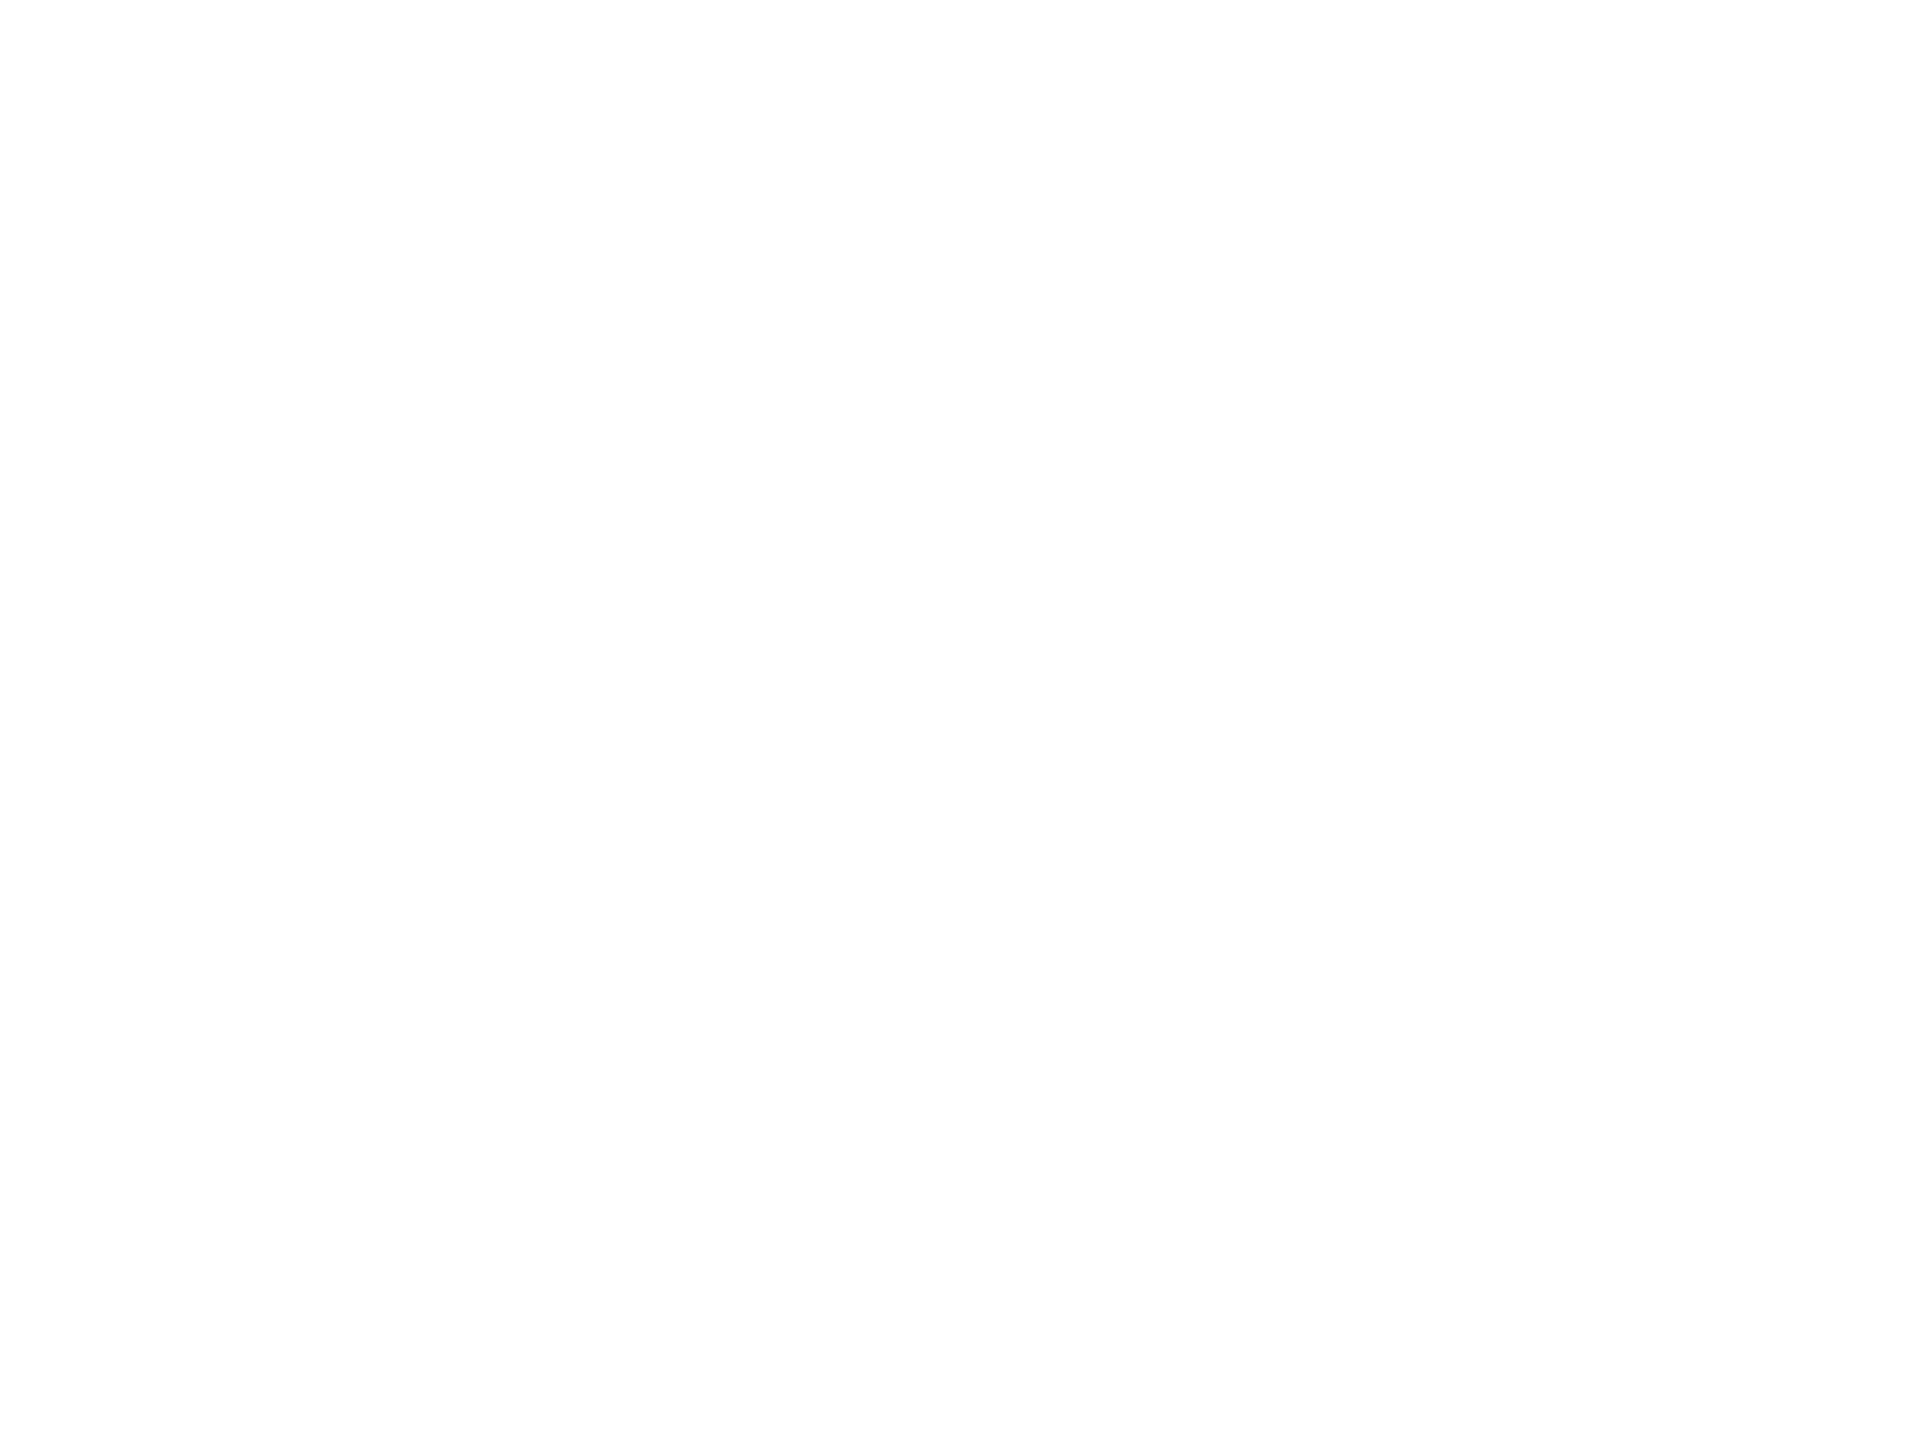
\includegraphics[width=1\linewidth]{figure/NSbox18-1} \end{center}

\hypertarget{binary-to-hexadecimal-conversion}{%
\subsubsection{Binary-to-Hexadecimal Conversion}\label{binary-to-hexadecimal-conversion}}

\begin{itemize}
\tightlist
\item
  To convert from binary to Hexadecimal, subdivide the number into groups of four bits. The hexadecimal representation of each group then gives the hexadecimal representation.
\end{itemize}

\textbf{Example 1: Convert the binary number 11010101.01101 to its Hexadecimal equivalent}

\begin{center}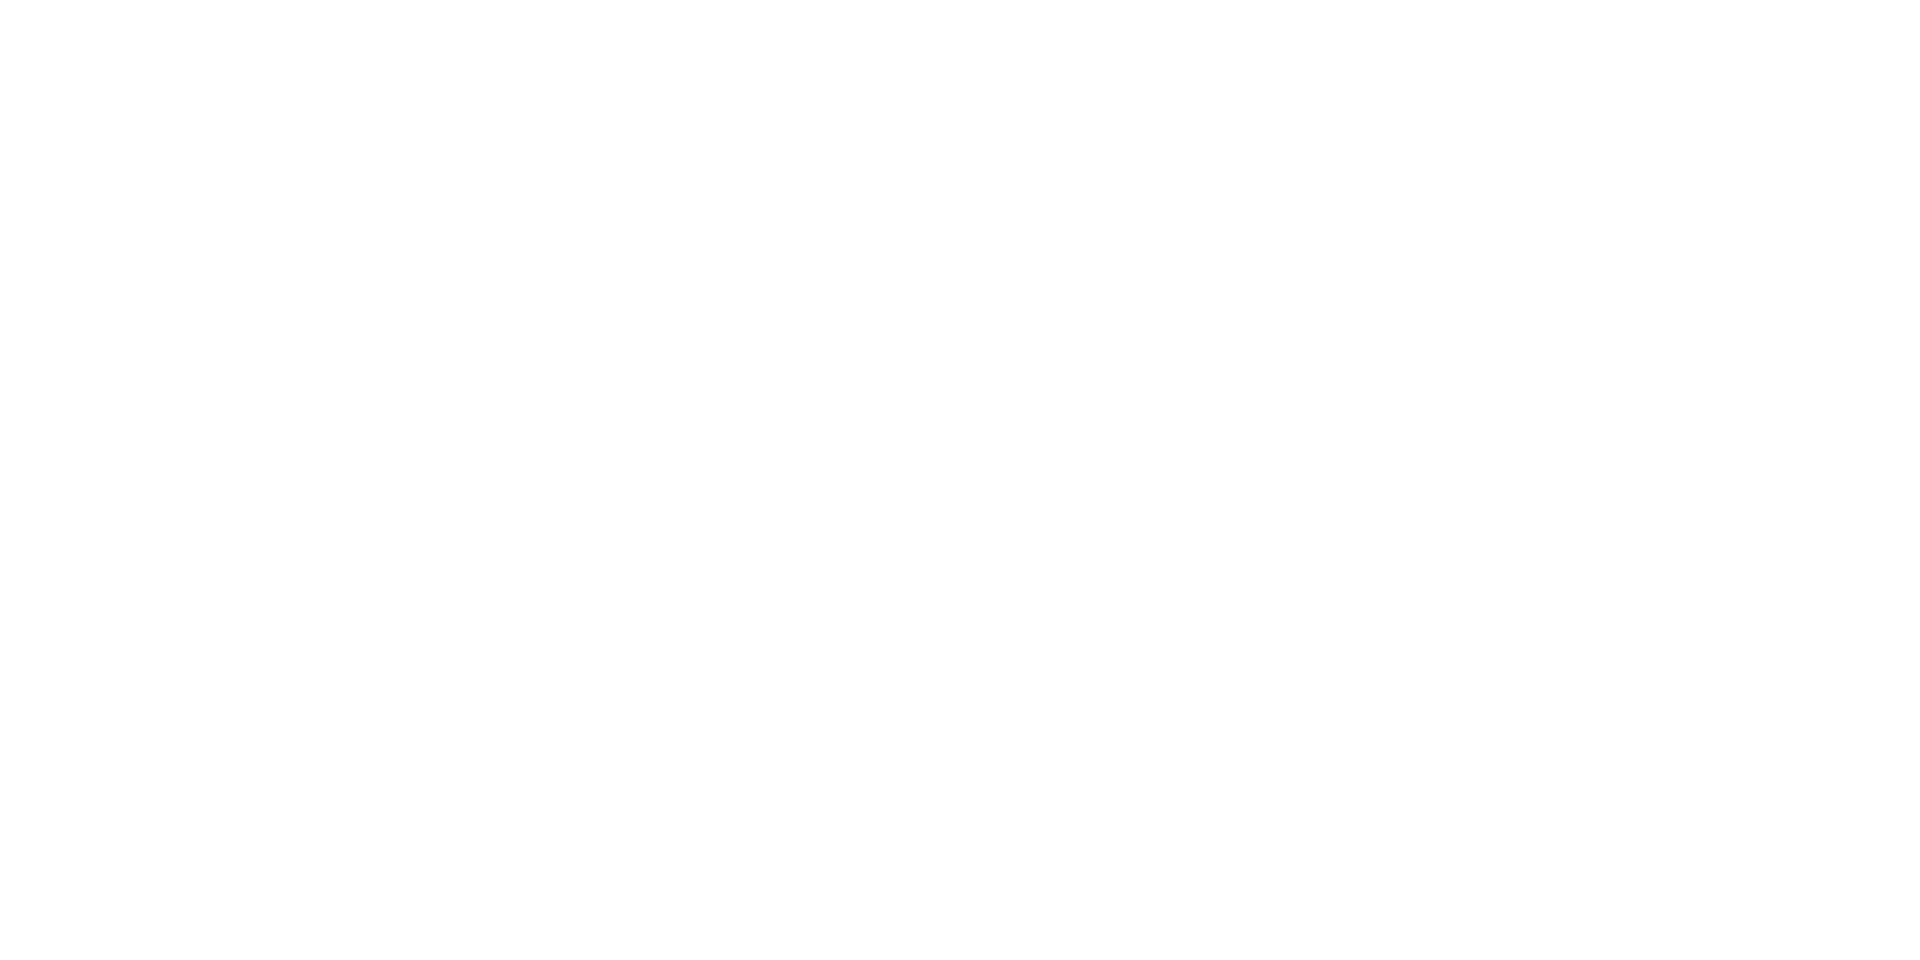
\includegraphics[width=1\linewidth]{figure/NSbox19-1} \end{center}

\hypertarget{octal-to-hexadecimal-conversion}{%
\subsubsection{Octal-to-Hexadecimal Conversion}\label{octal-to-hexadecimal-conversion}}

\begin{itemize}
\tightlist
\item
  First convert octal to binary, and then convert binary to hexadecimal.
\end{itemize}

\textbf{Example 1: Convert the octal number 365.52 to its Hexadecimal equivalent}

\begin{center}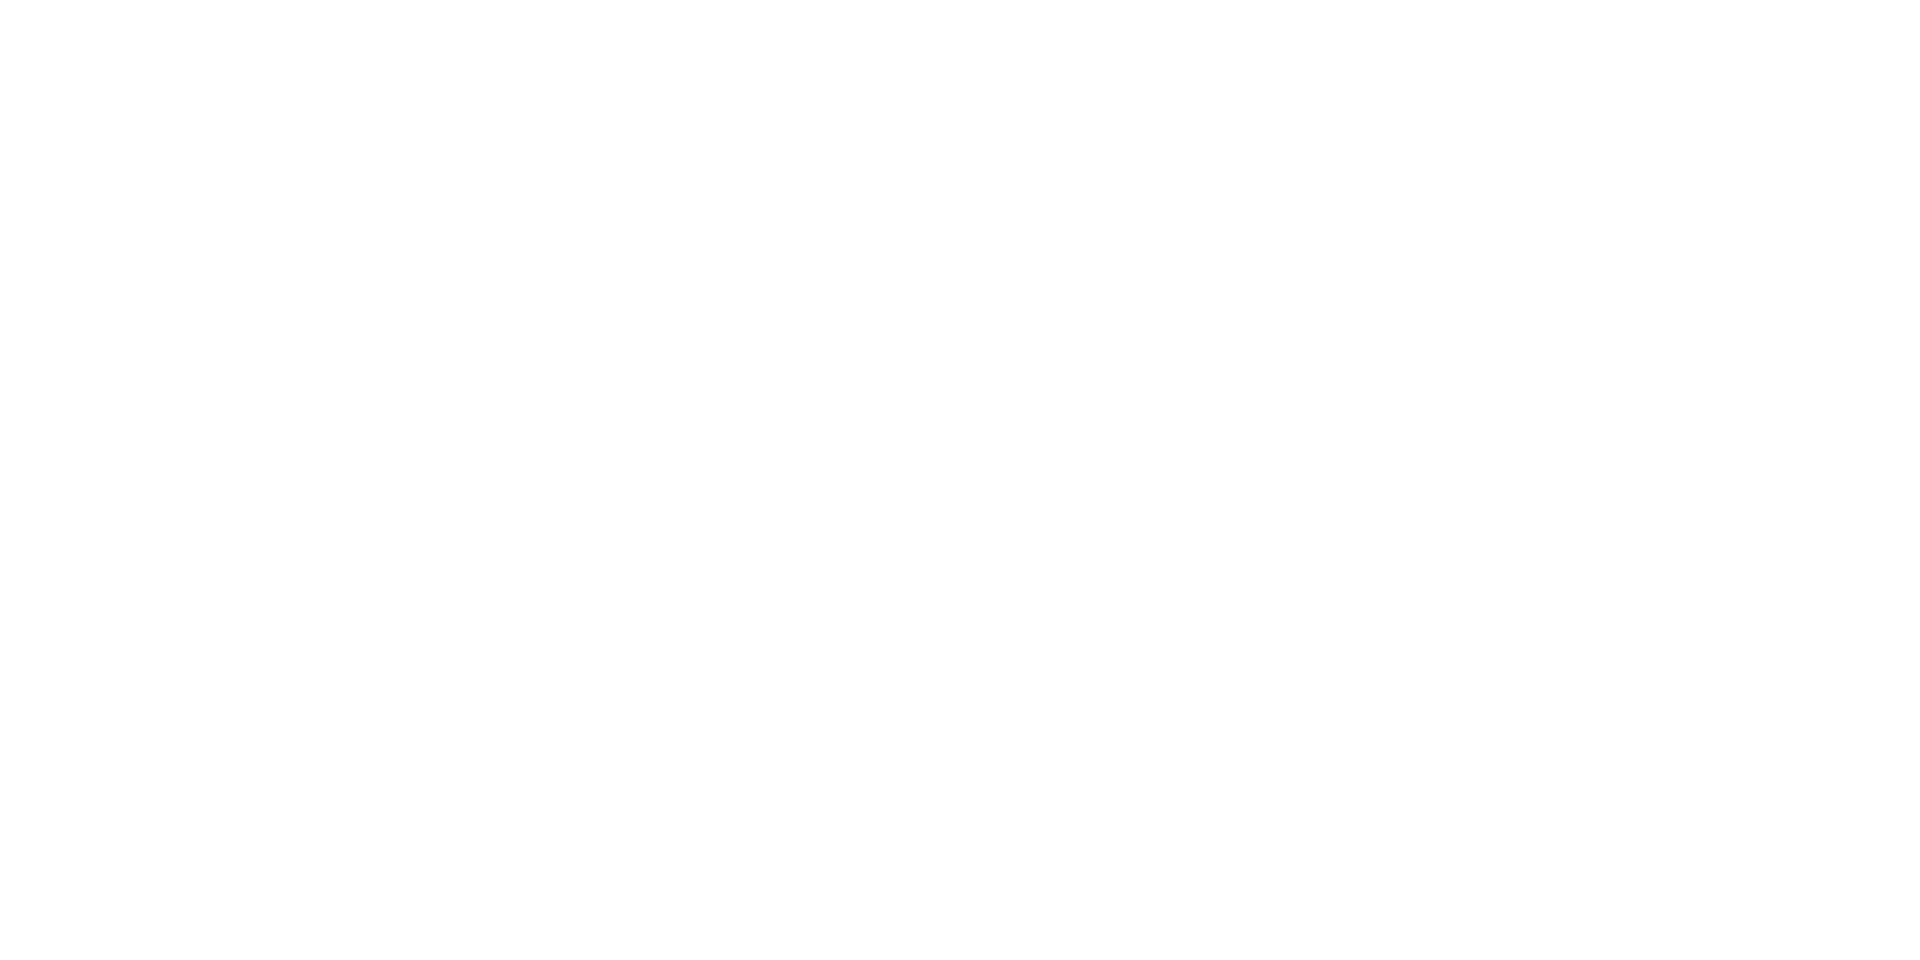
\includegraphics[width=1\linewidth]{figure/NSbox20-1} \end{center}

\hypertarget{hexadecimal-to-octal-conversion}{%
\subsubsection{Hexadecimal-to-octal conversion}\label{hexadecimal-to-octal-conversion}}

\begin{itemize}
\tightlist
\item
  First convert Hexadecimal to binary, and then convert binary to octal.
\end{itemize}

\textbf{Example 1: Convert the octal number D2B.284 to its Hexadecimal equivalent}

\begin{center}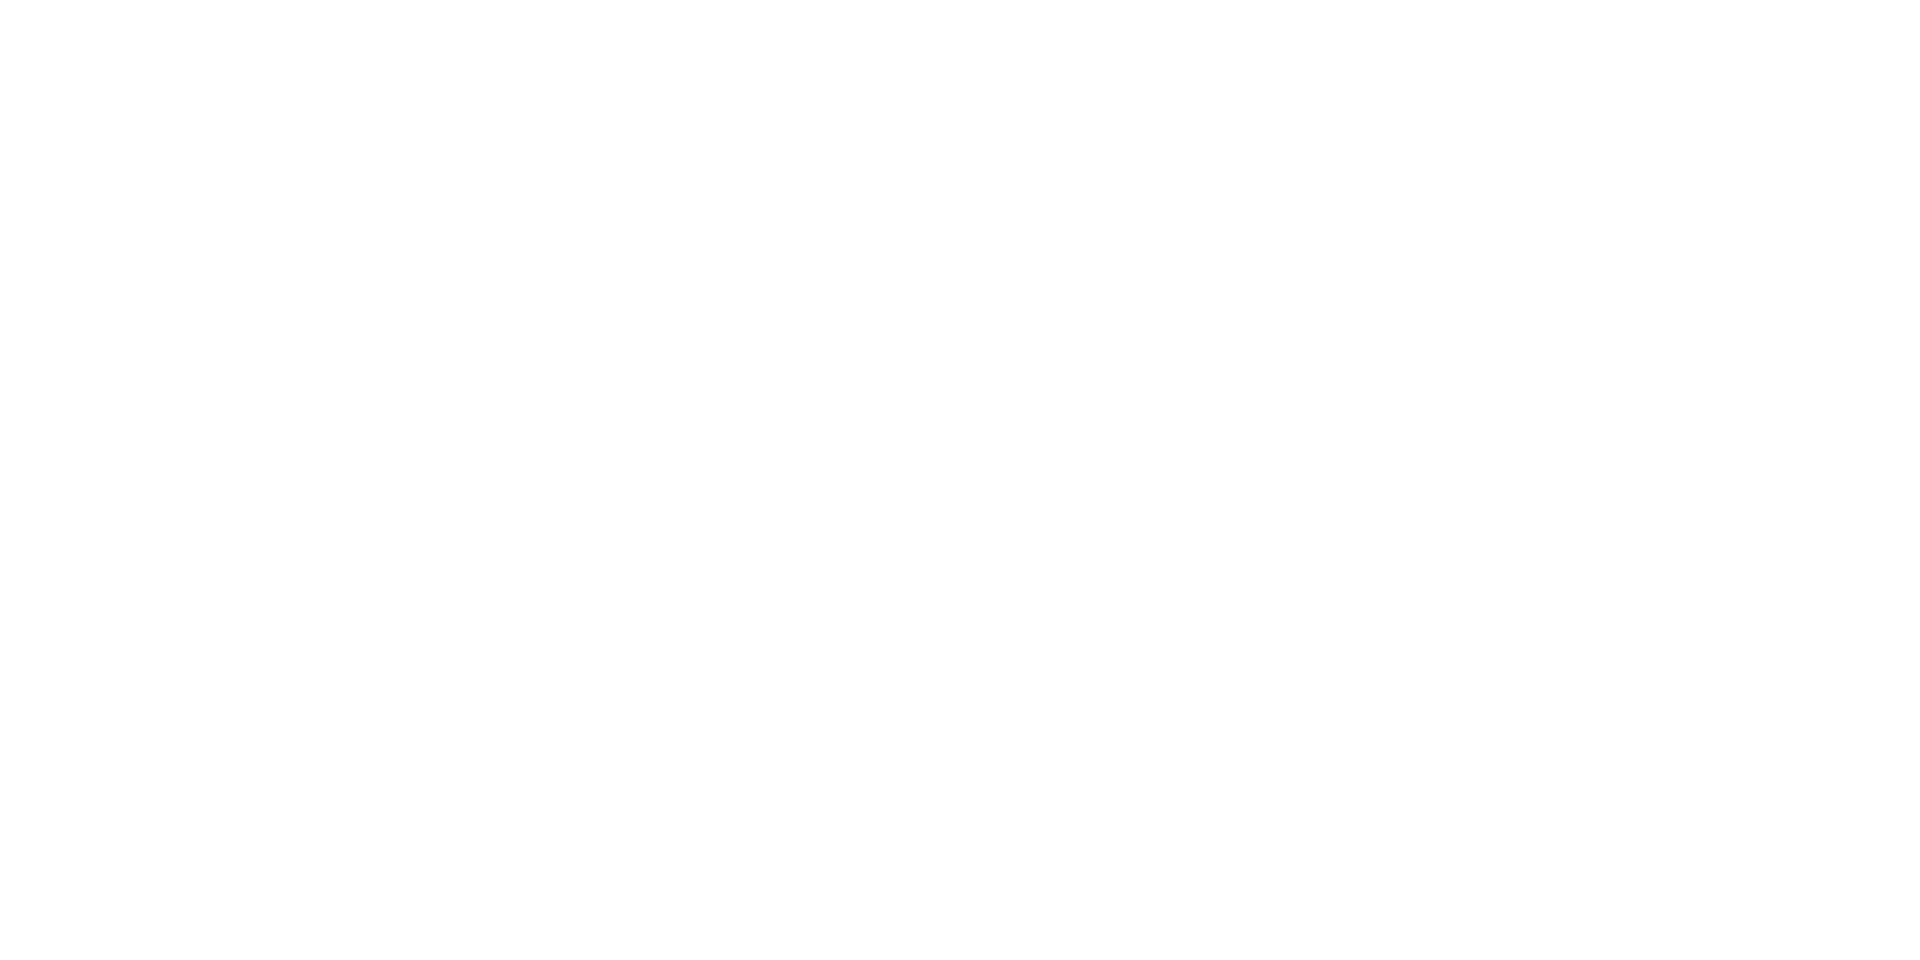
\includegraphics[width=1\linewidth]{figure/NSbox21-1} \end{center}

\hypertarget{binary-arithmetic}{%
\subsection{Binary Arithmetic}\label{binary-arithmetic}}

The arithmetic operations: addition, subtraction, multiplication and division of binary numbers follow the rules as summarized below

\begin{longtable}[]{@{}llll@{}}
\toprule
Addition & Subtraction & Multiplication & Division\tabularnewline
\midrule
\endhead
\(0+0 = 0\) & \(0-0=0\) & \(0\times0=0\) & \(\frac{0}{1} = 0\)\tabularnewline
\(0+1 = 1\) & \(1-0=1\) & \(0\times1=0\) & \(\frac{1}{1} = 1\)\tabularnewline
\(1+0 = 1\) & \(1-1 = 0\) & \(1\times0=0\) & \(\frac{0}{0} = undefined\)\tabularnewline
\(1+1 = 10\) & \(1-0 = 10-1 =1\) & \(1\times1=1\) & \(\frac{1}{0} = undefined\)\tabularnewline
\bottomrule
\end{longtable}

\hypertarget{binary-addition}{%
\subsubsection{Binary Addition}\label{binary-addition}}

\textbf{Example 1: Add (a) 111 and 101 (b) 1010, 1001 and 1101}

\begin{center}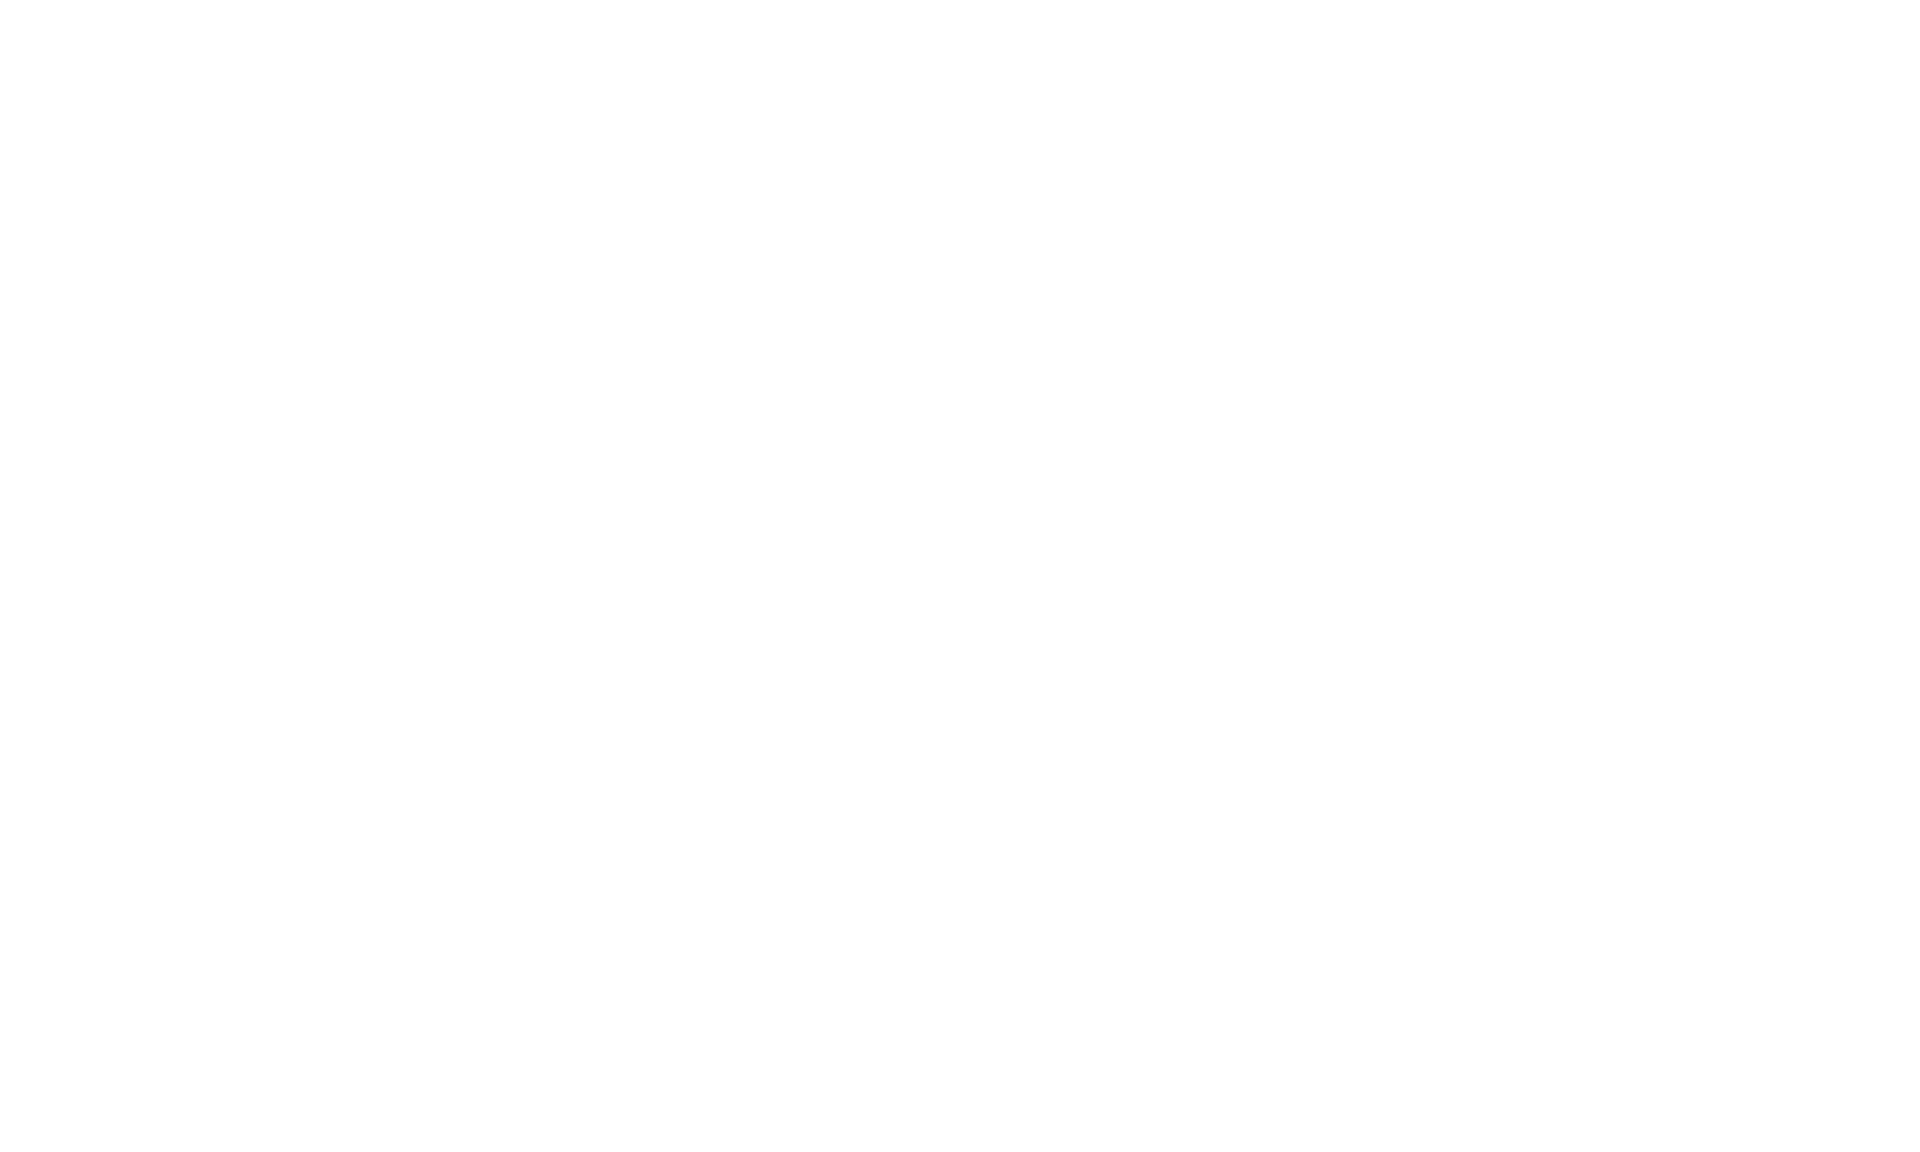
\includegraphics[width=1\linewidth]{figure/NSbox22-1} \end{center}

\hypertarget{binary-subtraction}{%
\subsubsection{Binary Subtraction}\label{binary-subtraction}}

\textbf{Example 1: Perform the following subtractions}

\begin{enumerate}
\def\labelenumi{(\alph{enumi})}
\tightlist
\item
  \(11- 01\) (b) \(11-10\) (c) \(100-011\)
\end{enumerate}

\begin{center}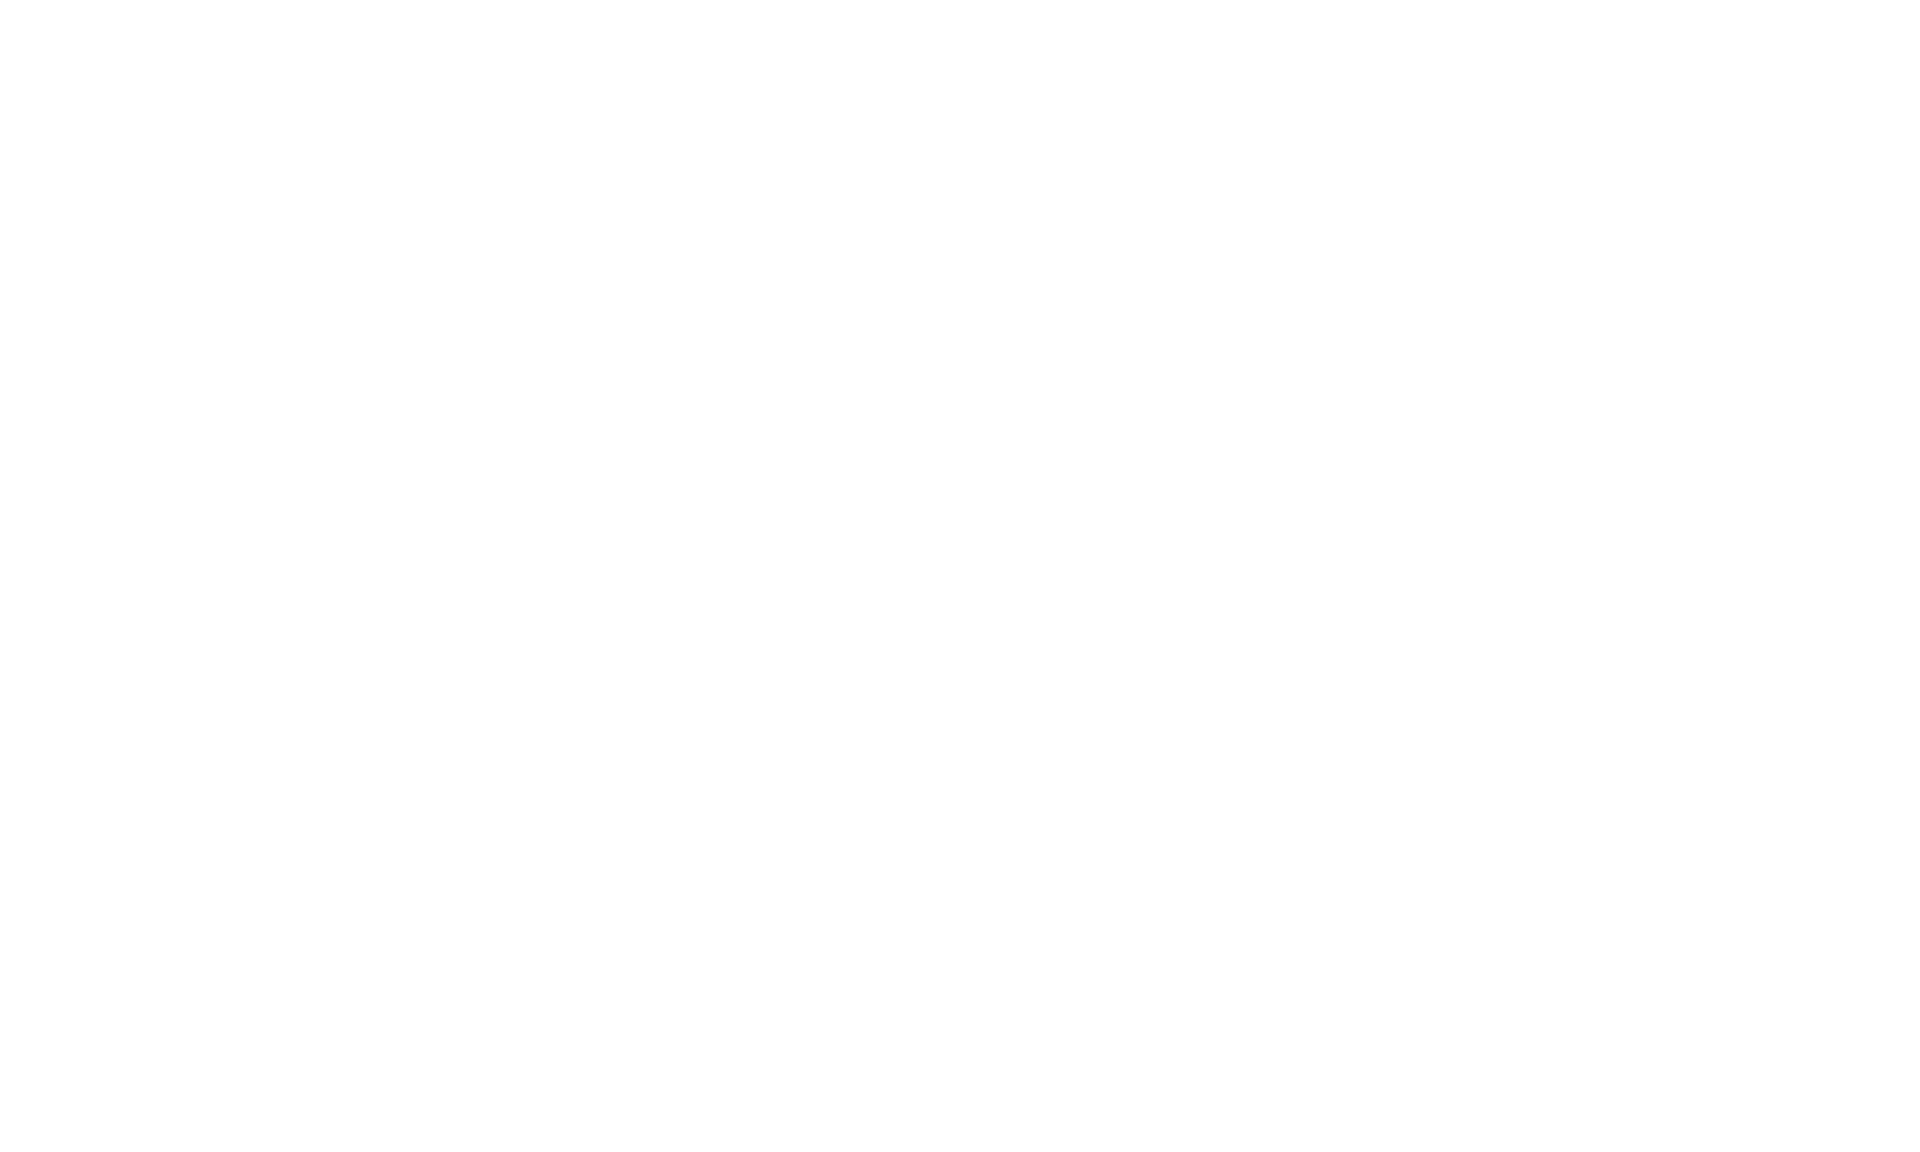
\includegraphics[width=1\linewidth]{figure/NSbox23-1} \end{center}

\begin{itemize}
\tightlist
\item
  When subtracting a larger number from a smaller number, the output will be negative.
\item
  To perform this subtraction, subtract the smaller number from the larger number and prefix the output with the sign of the larger number.
\end{itemize}

\textbf{Example 2: Perform the following subtraction 101 - 111}

\begin{center}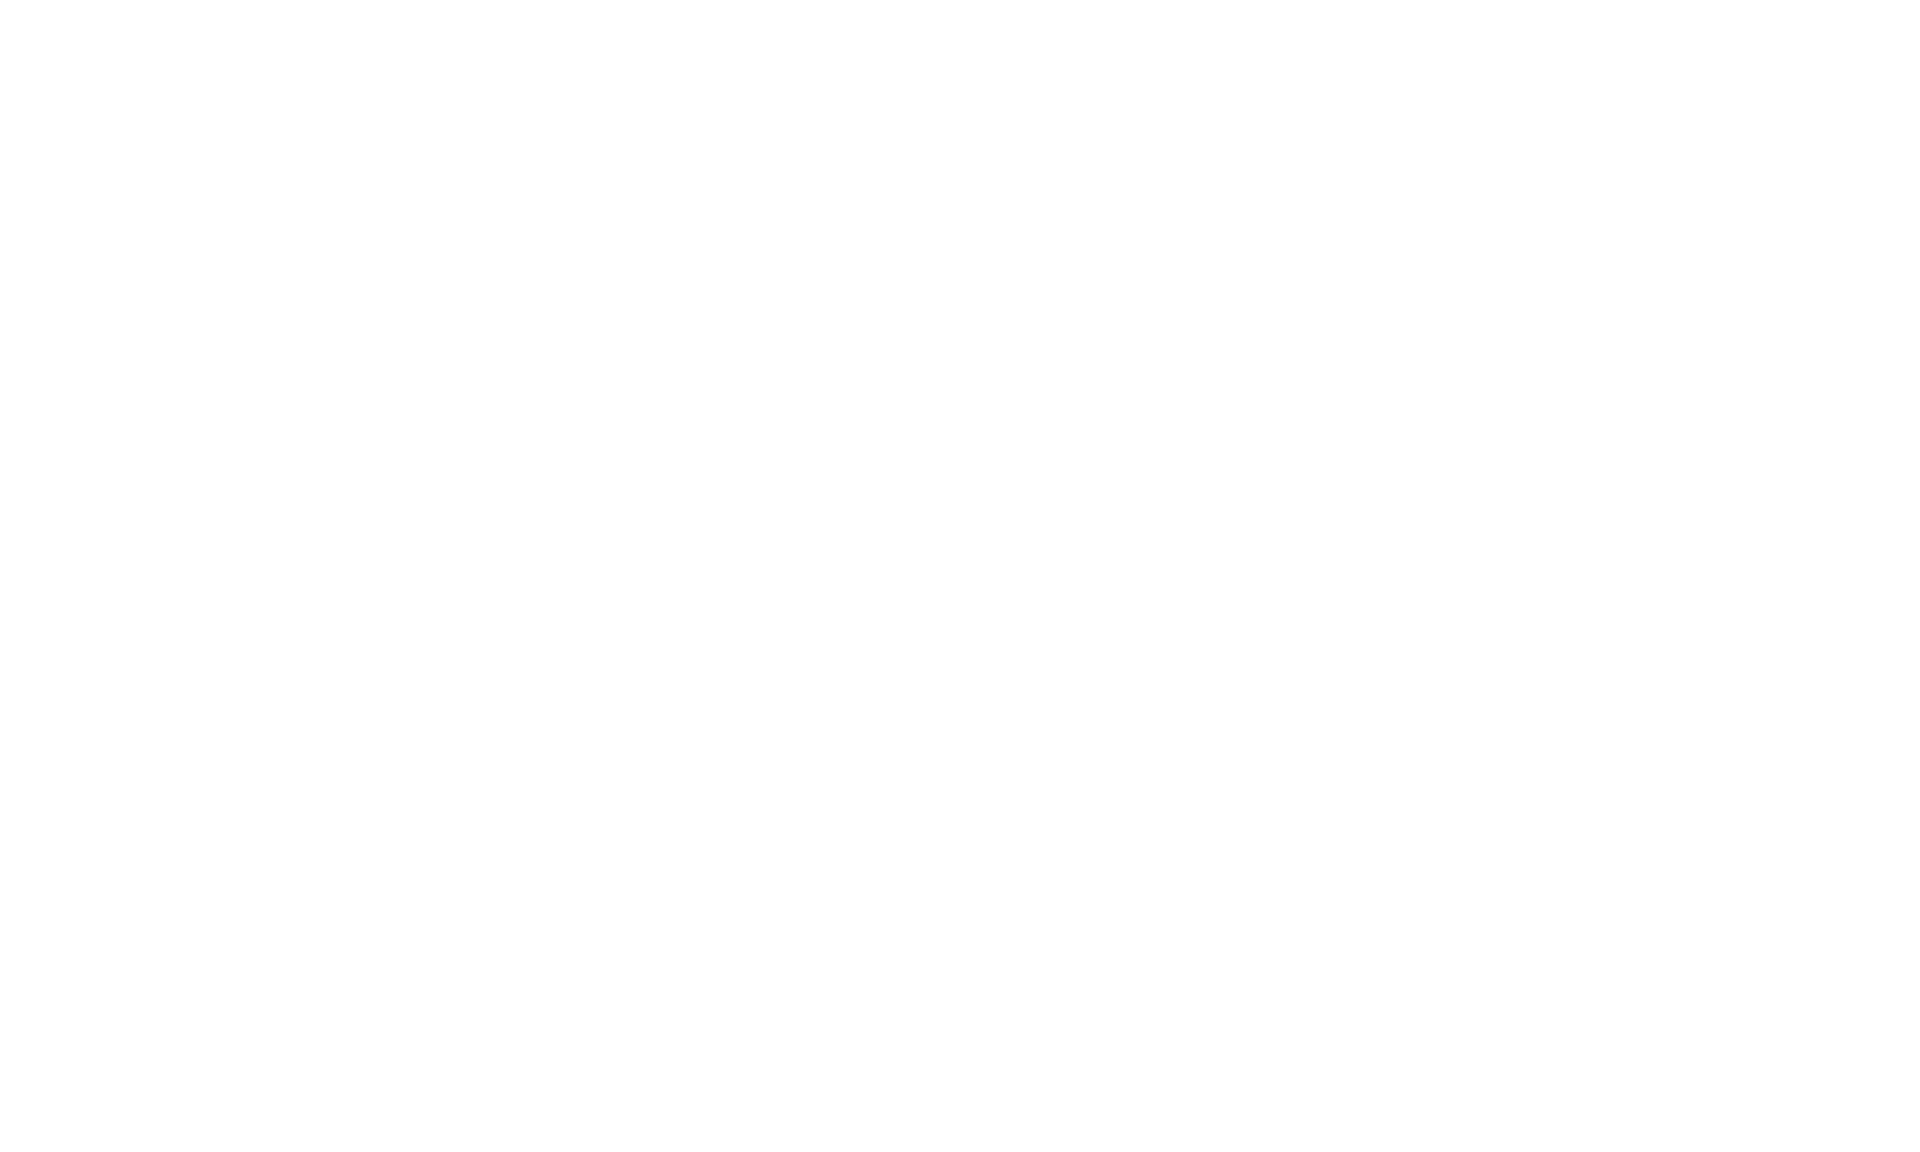
\includegraphics[width=1\linewidth]{figure/NSbox24-1} \end{center}

\hypertarget{binary-multiplication}{%
\subsubsection{Binary multiplication}\label{binary-multiplication}}

\textbf{Example 1: Multiply the following binary numbers}

\begin{enumerate}
\def\labelenumi{(\alph{enumi})}
\tightlist
\item
  \(101\times11\) (b) \(1101\times10\) (c) \(1010\times101\)
\item
  \(1011\times1010\)
\end{enumerate}

\begin{center}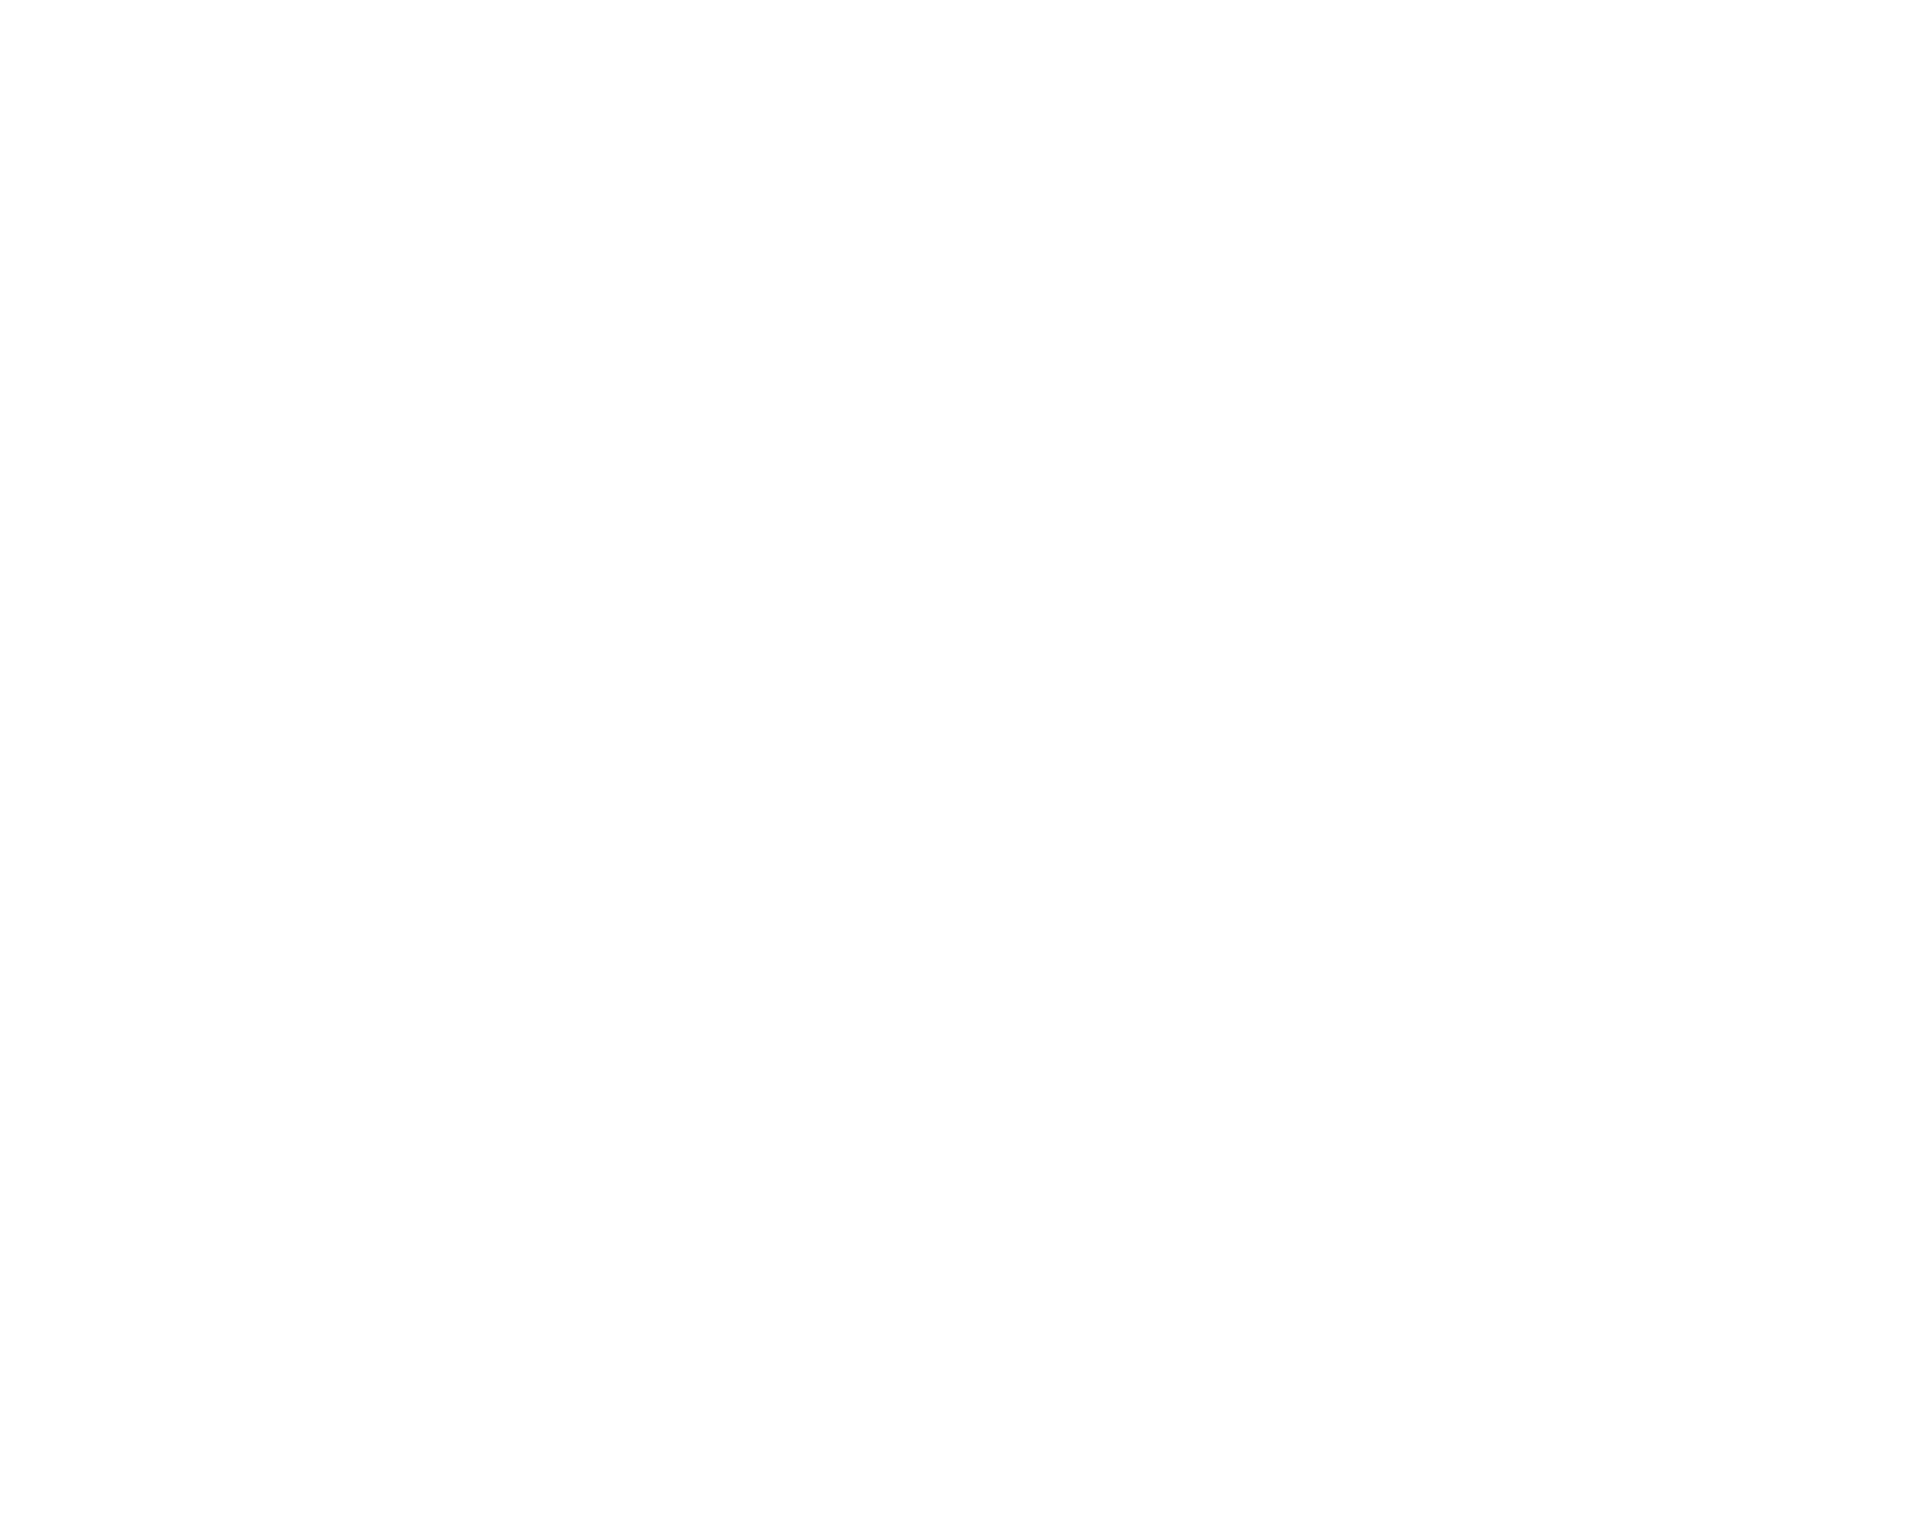
\includegraphics[width=1\linewidth]{figure/NSbox25-1} \end{center}

\begin{itemize}
\tightlist
\item
  Multiplication of factional numbers is perform in the same manner as with decimal factional numbers.
\end{itemize}

\textbf{Example 2: Perform the binary multiplication} \(0.01\times11\)

\begin{center}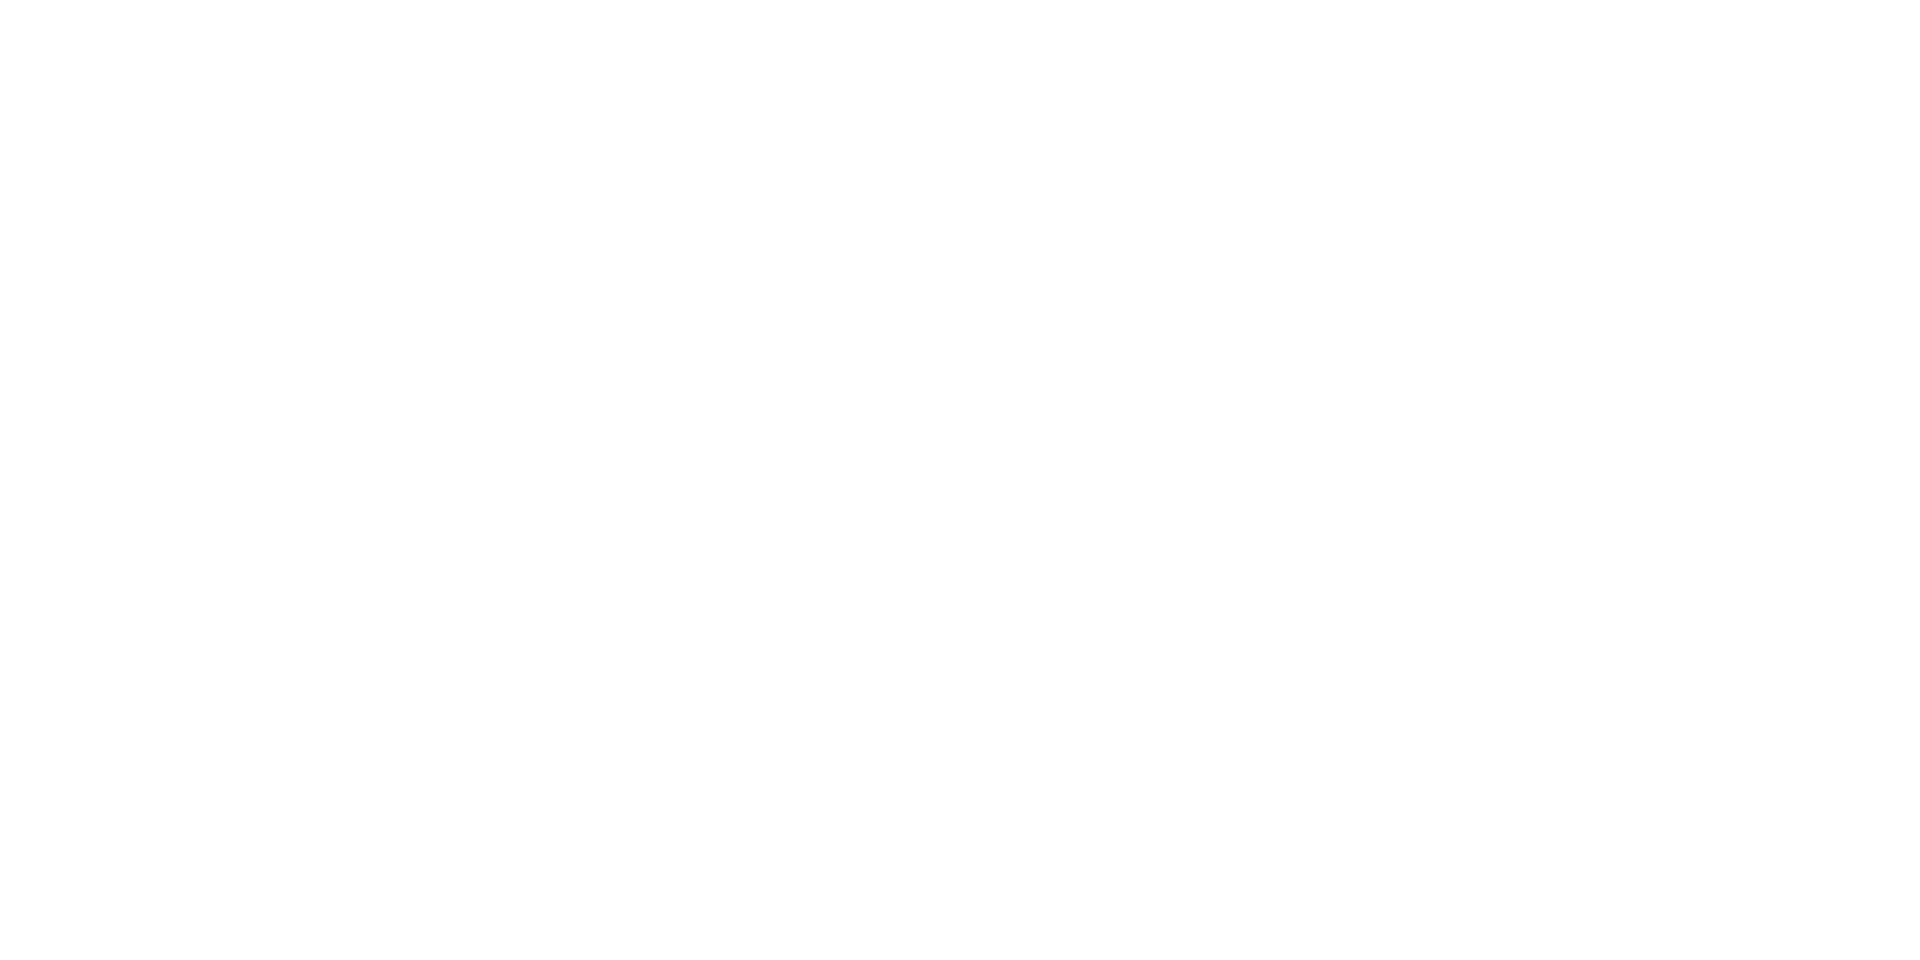
\includegraphics[width=1\linewidth]{figure/NSbox26-1} \end{center}

\hypertarget{binary-division}{%
\subsubsection{Binary Division}\label{binary-division}}

\textbf{Example 1: Perform the following binary division}

\begin{enumerate}
\def\labelenumi{(\alph{enumi})}
\tightlist
\item
  \(110\div11\) (b) \(1100\div11\) (c) \(1111\div110\) (d) \(1100\div101\)
\end{enumerate}

\begin{center}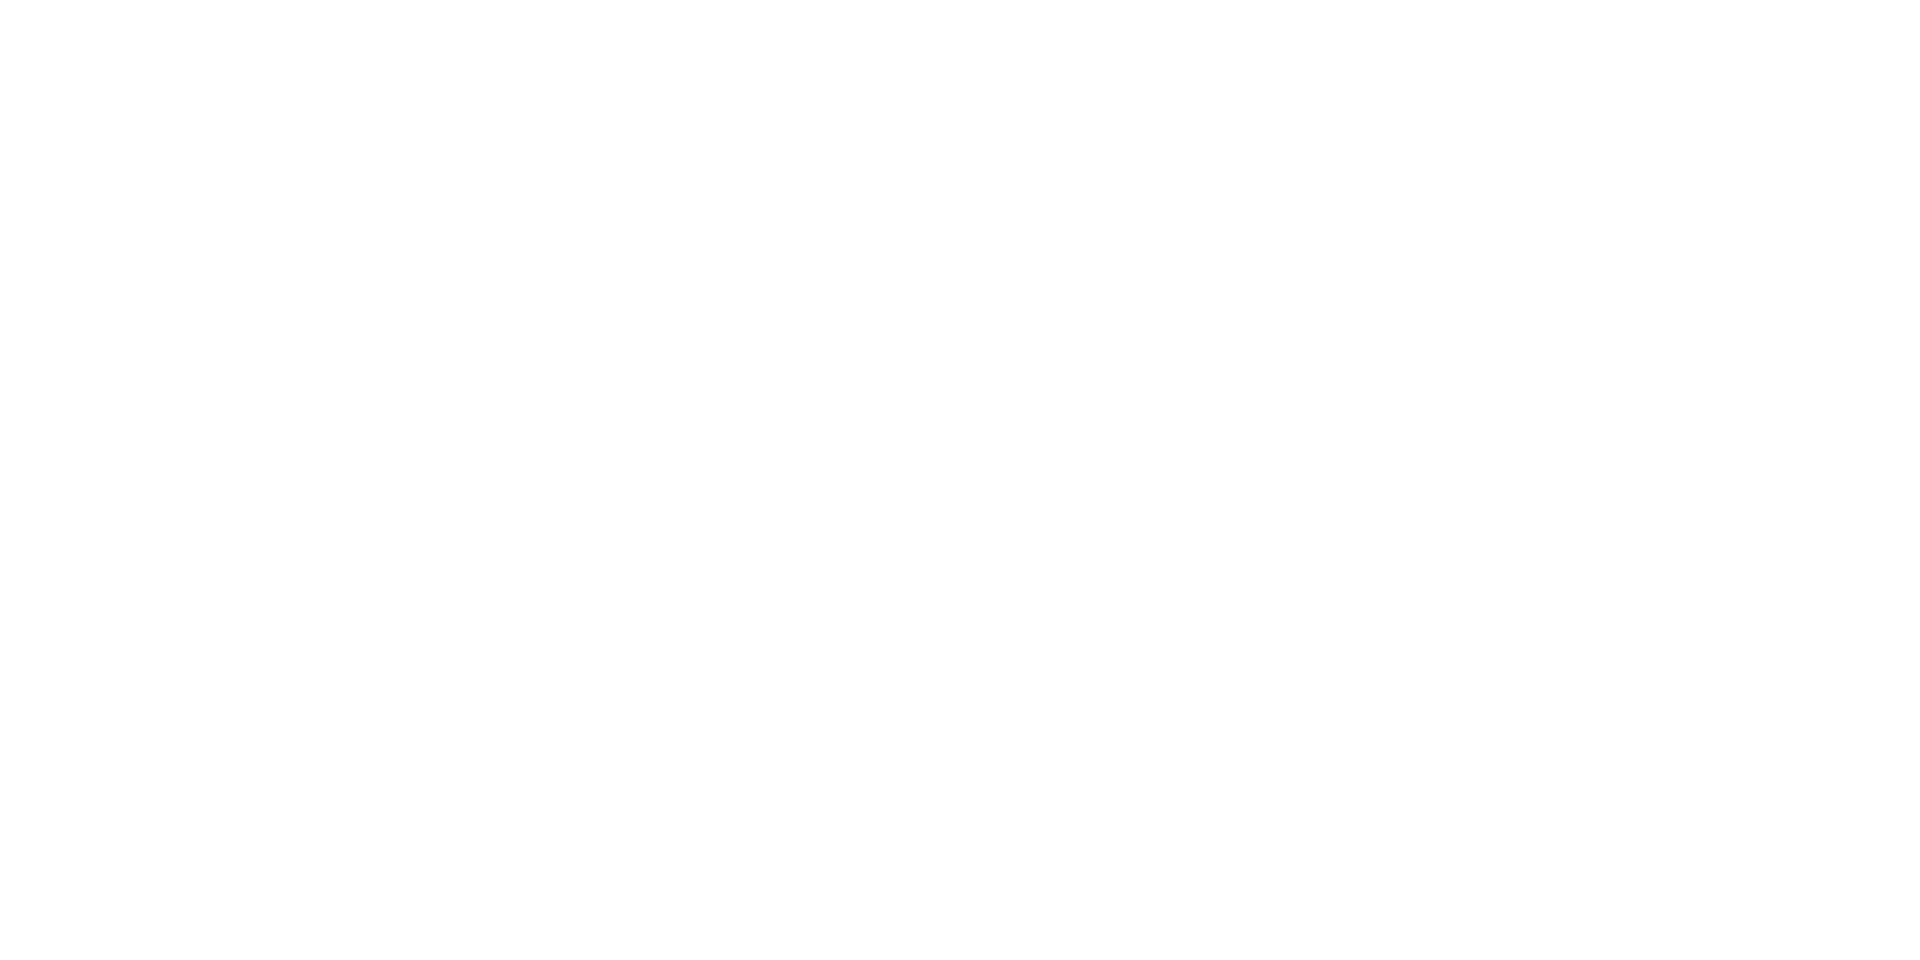
\includegraphics[width=1\linewidth]{figure/NSbox27-1} \end{center}

\begin{center}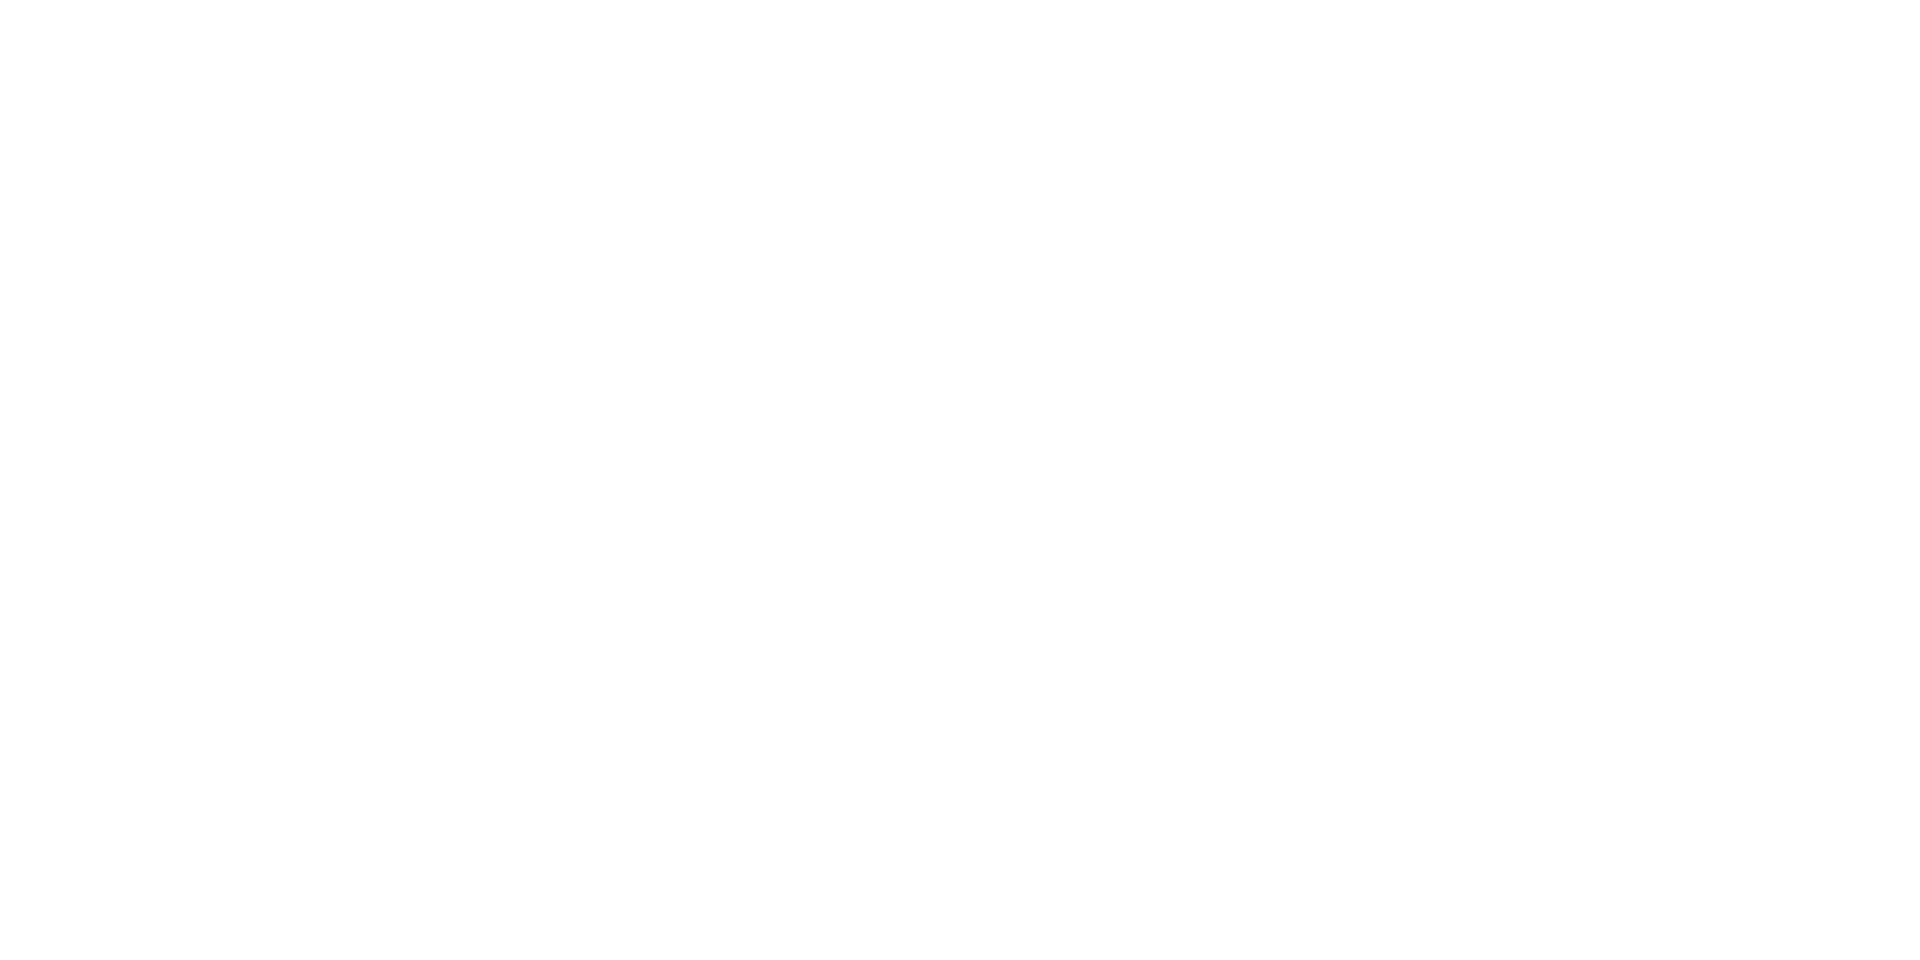
\includegraphics[width=1\linewidth]{figure/NSbox28-1} \end{center}

\hypertarget{sequences-and-series}{%
\chapter{Sequences and Series}\label{sequences-and-series}}

\hypertarget{sequences}{%
\section{Sequences}\label{sequences}}

\begin{itemize}
\tightlist
\item
  A \textbf{Sequence} can be thought of as a list of numbers written in a definite order:
  \[a_{1}, a_{2}, a_{3}, a_{4}, ..., a_{n}, ...\]
\item
  The number \(a_{1}\) is called the \emph{first term}, \(a_{2}\) is the \emph{second term}, and in general \(a_{n}\) is called the \(n^{th}\) \emph{term}.
\item
  We will deal exclusively with infinite sequences and so each term \(a_{n}\) will have a successor \(a_{n+1}\)
\item
  Notice that for every positive integer \(n\) there is a corresponding number \(a_{n}\) and so a sequence can be defined as a function whose domain is the set of positive integers.
\item
  But we usually write \(a_{n}\) instead of the function notation \(f(n)\) for the value of the function at the number \(n\).
\item
  \textbf{Notation:} The sequence \(\{a_{1}, a_{2}, a_{3},...\}\) is also denoted by
  \[\{a_{n}\}\] or \[\{a_{n}\}_{n=1}^{\infty}\]
\item
  Some sequences can be defined by giving a formula for the \(n\)th term.
\item
  In the following examples we give three descriptions of the sequences:

  \begin{enumerate}
  \def\labelenumi{\roman{enumi}.}
  \tightlist
  \item
    by using the preceding notation
  \item
    by using the defining formula
  \item
    by writing out the terms of the sequence
  \end{enumerate}
\item
  Notice that \(n\) doesn't have to start at 1.
\end{itemize}

\begin{enumerate}
\def\labelenumi{\alph{enumi})}
\item
  \(\{\frac{n}{n+1}\}_{n=1}^{\infty} \hspace{5em} a_{n} = \frac{n}{n+1}\hspace{5em}\{\frac{1}{2},\frac{2}{3}, \frac{3}{4}, \frac{4}{5},..., \frac{n}{n+1},... \}\)
\item
  \(\{\frac{(-1)^n(n+1)}{3^{n}}\}_{n=1}^{\infty} \hspace{5em} a_{n} = \frac{(-1)^n(n+1)}{3^{n}}\hspace{5em}\{-\frac{2}{3},\frac{3}{9}, -\frac{4}{27}, \frac{5}{81},..., \frac{(-1)^n(n+1)}{3^{n}},... \}\)
\item
  \(\{\sqrt{n-3}\}_{n=3}^{\infty} \hspace{5em} a_{n} = \sqrt{n-3}, n\geq3\hspace{5em}\{0,1,\sqrt{2}, \sqrt{3},..., \sqrt{n-3},...\}\)
\item
  \(\{cos\frac{n\pi}{6}\}_{n=0}^{\infty} \hspace{5em} a_{n} = cos\frac{n\pi}{6}, n\geq 0 \hspace{5em}\{1, \frac{\sqrt{3}}{2},\frac{1}{2}, 0,...,cos\frac{n\pi}{6},...\}\)
\end{enumerate}

\textbf{Example}

Find a formula for the general term \(a_{n}\) of the sequence
\[\{\frac{3}{5},-\frac{4}{25}, \frac{5}{125}, -\frac{6}{625}, \frac{7}{3125},...\}\]
assuming that the pattern of the first few terms continues.

\emph{SOLUTION}

We are given that

\hypertarget{series}{%
\section{Series}\label{series}}

Reading:

Stewart, J., Clegg, D. K., \& Watson, S. (2020). `Infinite Sequences and Series', \emph{Calculus: early transcendentals}. Cengage Learning.

\hypertarget{introduction-to-logic}{%
\chapter{Introduction to Logic}\label{introduction-to-logic}}

\hypertarget{boolean-algebra}{%
\chapter{Boolean Algebra}\label{boolean-algebra}}

\hypertarget{differentiation-and-integration}{%
\chapter{Differentiation and Integration}\label{differentiation-and-integration}}

\hypertarget{descriptive-statistics}{%
\chapter{Descriptive Statistics}\label{descriptive-statistics}}

\pagenumbering{arabic}

\hypertarget{introduction-to-statistics}{%
\section{Introduction to Statistics}\label{introduction-to-statistics}}

\hypertarget{some-basic-terminologies-used-in-statistics}{%
\subsection{Some Basic Terminologies Used in Statistics}\label{some-basic-terminologies-used-in-statistics}}

\textbf{i Population}

\begin{itemize}
\tightlist
\item
  The set of \textbf{all} possible elements in the universe of interest to the researcher
\end{itemize}

\textbf{ii Sample}

\begin{itemize}
\tightlist
\item
  A Sample is a \textbf{subset} (a portion or part) of the population of interest
\item
  The sample must be a representative of the population of interest
\end{itemize}

\textbf{iii Element}

\begin{itemize}
\tightlist
\item
  Element is an \textbf{entity or object} which the information is collected.
\item
  \emph{Eg: Student, household, farm, company, tomato plant}
\end{itemize}

\textbf{iv Variable}

\begin{itemize}
\tightlist
\item
  A variable is \textbf{a feature characteristic which has different `values' or categories for different elements} (items/subjects/individuals)
\item
  \emph{Eg: Gender of client, brand of mobile phones, risk level, number of emails received per day, age of client, income of client}
\end{itemize}

\textbf{v Data}

\begin{itemize}
\item
  Data are \textbf{measurements or facts} that are collected from a statistical unit/entity of interest
\item
  We collect data on variables
\item
  Data are raw numbers or facts that must be processed (analysed) to get useful information.
\item
  We get information from data.
\item
  \emph{Eg:}
\end{itemize}

\textbf{\emph{Variable:}} \emph{Age (in years) of client}

\textbf{\emph{Data:}} \emph{21, 45, 18, 32, 30, 22, 23, 27}

\textbf{\emph{Information:}}

\emph{The mean age is 27.25 years}

\emph{The minimum age is 18 years}

\emph{The range of ages is 18-45}

\emph{The percentage of clients below 25 years of age: 50\%}

\textbf{vi Statistic}

\begin{itemize}
\tightlist
\item
  \textbf{Characteristic} of a \textbf{sample}
\item
  The value which calculated based on sample data
\end{itemize}

\textbf{vii Parameter}

\begin{itemize}
\tightlist
\item
  \textbf{Characteristic} of a \textbf{population}
\item
  The value which calculated based on population data
\end{itemize}

\textbf{viii Census}

\begin{itemize}
\tightlist
\item
  When a researcher \textbf{gathers data from the whole population for a given measurement,} it is called a census
\end{itemize}

\textbf{ix Sampling}

\begin{itemize}
\tightlist
\item
  When a researcher \textbf{gathers data from a sample of the population for a given measurement,} it is called sampling
\item
  The process of selecting a sample is also called sampling
\end{itemize}

\textbf{Why take a sample instead of studying every member of the population ?}

\begin{itemize}
\tightlist
\item
  Prohibitive cost of census
\item
  Destruction of item being studied may be required
\item
  Not possible to test or inspect all members of a population being studied.
\end{itemize}

\hypertarget{branches-of-statistics}{%
\subsection{Branches of Statistics}\label{branches-of-statistics}}

\begin{figure}

{\centering 
\includegraphics[width=1\linewidth]{figure/box1-1} 

}

\end{figure}

\textbf{i Descriptive Statistics}

\begin{itemize}
\tightlist
\item
  Descriptive statistics consists of organizing, summarizing and presenting data in an informative way.
\item
  The main purpose of descriptive statistics is to provide an overview of the data collected.
\item
  Descriptive statistics describes the data collected through frequency tables, graphs and summary measures (mean, variance, quartiles, etc.).
\end{itemize}

\textbf{ii Inferential Statistics}

\begin{itemize}
\tightlist
\item
  In inferential statistics sample data are used to draw inferences (i.e.~derive conclusions) or make predictions about the populations from which the sample has been taken.
\item
  This includes methods used to make decisions, estimates, predictions or generalizations about a population based on a sample.
\item
  This includes point estimations, interval estimation, test of hypotheses, regression analysis, time series analysis, multivariate analysis, etc.
\end{itemize}

\hypertarget{types-of-variables}{%
\subsection{Types of Variables}\label{types-of-variables}}

\begin{figure}

{\centering 
\includegraphics[width=1\linewidth]{figure/box2-1} 

}

\end{figure}

\hypertarget{qualitative-quantitative-variables}{%
\subsubsection{Qualitative / Quantitative Variables}\label{qualitative-quantitative-variables}}

\textbf{i Qualitative variable (Categorical variable)}

\begin{itemize}
\tightlist
\item
  The characteristic is a quality.
\item
  The data are categories.
\item
  They cannot be given numerical values.
\item
  However, it may be given a numerical label
\item
  Qualitative variables are sometimes referred as categorical variables.
\item
  \emph{Eg:}
\end{itemize}

\emph{Gender:}

\emph{Age group:}

\emph{Education level:}

\emph{A/L stream:}

\emph{Degree type:}

\emph{Hair colour: }

\emph{FIT student batch:}

\emph{Undergraduate level:}

\emph{Grade that you can obtain for CM 1110/ CM1130}

\textbf{ii Quantitative variable }

\begin{itemize}
\tightlist
\item
  The characteristic is a quantity
\item
  The data are numbers
\item
  Quantitative data require numeric values that indicate how much or how many.
\item
  They are obtained by counting or measuring with some scale
\item
  \emph{Eg: }
\end{itemize}

\emph{Number of family members:}

\emph{Number of emails received per day:}

\emph{Weight of a student:}

\emph{Age:}

\emph{Credit balance in the SIM card:}

\emph{Time remaining in class:}

\emph{Temperature:}

\emph{Marks }

\hypertarget{discrete-continuous-variables}{%
\subsubsection{Discrete/ Continuous Variables}\label{discrete-continuous-variables}}

\begin{itemize}
\tightlist
\item
  Quantitative variables can be classified as either discrete or continuous.
\end{itemize}

\textbf{i Discrete Variables}

\begin{itemize}
\tightlist
\item
  Quantitative
\item
  Usually the data are obtained by counting
\item
  There are impossible values between any two possible values
\item
  \emph{Eg:}
\end{itemize}

\emph{Number of family members:}

\emph{Number of emails received per day:}

\textbf{ii Continuous Variables}

\begin{itemize}
\tightlist
\item
  Quantitative
\item
  Usually, the data are obtained by measuring with a scale
\item
  There are no impossible values between any two possible values.(any value between any two possible values is also a possible value)
\item
  i.e a continuous variable can take any value within a specified range.
\item
  \emph{Eg:}
\end{itemize}

\emph{Weight of a student:}

\emph{Age:}

\emph{Credit balance in the SIM card:}

\emph{Time remaining in class:}

\emph{Temperature:}

\emph{Marks}

\hypertarget{scales-of-measurements}{%
\subsection{Scales of Measurements}\label{scales-of-measurements}}

\begin{figure}

{\centering 
\includegraphics[width=1\linewidth]{figure/box3-1} 

}

\end{figure}

\begin{itemize}
\tightlist
\item
  There are four levels of measurements called, \textbf{nominal, ordinal, interval and ratio.}
\item
  Each levels has its own rules and restrictions
\item
  Different levels of measurement contains different amount of information with respect to whatever the data are measuring
\end{itemize}

\textbf{i Nominal Scale}

\begin{itemize}
\tightlist
\item
  Qualitative
\item
  No order or ranking in categories.
\item
  These categories have to be mutually exclusive, i.e.~it should not be possible to place an individual or object in more than one category
\item
  A name of a category can be substituted by a number, but it will be mere label and have no numerical meaning
\end{itemize}

\textbf{ii Ordinal Scale}

\begin{itemize}
\tightlist
\item
  Qualitative
\item
  Categories can be ordered or ranked
\item
  A name of a category can be substituted by a number, but such a sequence does not indicate absolute quantities.
\item
  Difference between any two numbers on the scale does not have a numerical meaningful.
\item
  It cannot be assumed that the differences between adjacent numbers on the scale are equal.
\end{itemize}

\textbf{iii Interval Scale}

\begin{itemize}
\tightlist
\item
  Quantitative
\item
  Data can be ordered or ranked
\item
  There is no absolute zero point. Zero is only an arbitrary point with which other values can compare
\item
  Difference between two numbers is a meaningful numerical value
\item
  Ration of two numbers is not a meaningful numerical value.
\end{itemize}

\textbf{iv Ratio Scale}

\begin{itemize}
\tightlist
\item
  Quantitative
\item
  Highest level of measurement
\item
  There exist an absolute zero point (It has a true zero point)
\item
  Ratio between different measurements is meaningful
\end{itemize}

\newpage

\hypertarget{presentation-of-data}{%
\section{Presentation of Data}\label{presentation-of-data}}

The sinking of the Titanic is one of the most infamous shipwrecks in history.

On April 15, 1912, during her maiden voyage, the widely considered ``unsinkable'' RMS Titanic sank after colliding with an iceberg. Unfortunately, there weren't enough lifeboats for everyone onboard, resulting in the death of 1502 out of 2224 passengers and crew

\footnote{Data source: \url{https://www.kaggle.com/varimp/a-mostly-tidyverse-tour-of-the-titanic}}

Here's a quick summary of our variables:

\begin{longtable}[]{@{}ll@{}}
\toprule
\begin{minipage}[b]{0.49\columnwidth}\raggedright
Variable Name\strut
\end{minipage} & \begin{minipage}[b]{0.45\columnwidth}\raggedright
Description\strut
\end{minipage}\tabularnewline
\midrule
\endhead
\begin{minipage}[t]{0.49\columnwidth}\raggedright
PassengerID\strut
\end{minipage} & \begin{minipage}[t]{0.45\columnwidth}\raggedright
Passenger ID (just a row number, so obviously not useful for prediction)\strut
\end{minipage}\tabularnewline
\begin{minipage}[t]{0.49\columnwidth}\raggedright
Survived\strut
\end{minipage} & \begin{minipage}[t]{0.45\columnwidth}\raggedright
Survived (1) or died (0)\strut
\end{minipage}\tabularnewline
\begin{minipage}[t]{0.49\columnwidth}\raggedright
Pclass\strut
\end{minipage} & \begin{minipage}[t]{0.45\columnwidth}\raggedright
Passenger class (first, second or third)\strut
\end{minipage}\tabularnewline
\begin{minipage}[t]{0.49\columnwidth}\raggedright
Name\strut
\end{minipage} & \begin{minipage}[t]{0.45\columnwidth}\raggedright
Passenger name\strut
\end{minipage}\tabularnewline
\begin{minipage}[t]{0.49\columnwidth}\raggedright
Gender\strut
\end{minipage} & \begin{minipage}[t]{0.45\columnwidth}\raggedright
Passenger Gender\strut
\end{minipage}\tabularnewline
\begin{minipage}[t]{0.49\columnwidth}\raggedright
Age\strut
\end{minipage} & \begin{minipage}[t]{0.45\columnwidth}\raggedright
Passenger age\strut
\end{minipage}\tabularnewline
\begin{minipage}[t]{0.49\columnwidth}\raggedright
SibSp\strut
\end{minipage} & \begin{minipage}[t]{0.45\columnwidth}\raggedright
Number of siblings/spouses aboard\strut
\end{minipage}\tabularnewline
\begin{minipage}[t]{0.49\columnwidth}\raggedright
Parch\strut
\end{minipage} & \begin{minipage}[t]{0.45\columnwidth}\raggedright
Number of parents/children aboard\strut
\end{minipage}\tabularnewline
\begin{minipage}[t]{0.49\columnwidth}\raggedright
Ticket\strut
\end{minipage} & \begin{minipage}[t]{0.45\columnwidth}\raggedright
Ticket number\strut
\end{minipage}\tabularnewline
\begin{minipage}[t]{0.49\columnwidth}\raggedright
Fare\strut
\end{minipage} & \begin{minipage}[t]{0.45\columnwidth}\raggedright
Fare\strut
\end{minipage}\tabularnewline
\begin{minipage}[t]{0.49\columnwidth}\raggedright
Cabin\strut
\end{minipage} & \begin{minipage}[t]{0.45\columnwidth}\raggedright
Cabin\strut
\end{minipage}\tabularnewline
\begin{minipage}[t]{0.49\columnwidth}\raggedright
Embarked\strut
\end{minipage} & \begin{minipage}[t]{0.45\columnwidth}\raggedright
Port of embarkation (S = Southampton, C = Cherbourg, Q = Queenstown)\strut
\end{minipage}\tabularnewline
\bottomrule
\end{longtable}

\hypertarget{tabular-presentations-of-data}{%
\subsection{Tabular Presentations of Data}\label{tabular-presentations-of-data}}

\textbf{Raw Data}

\begin{itemize}
\tightlist
\item
  Raw data are collected data that have not been organized numerically
\item
  Eg: Passenger age
\end{itemize}

\begin{verbatim}
##   PassengerId Survived Pclass
## 1           1        0      3
## 2           2        1      1
## 3           3        1      3
## 4           4        1      1
## 5           5        0      3
## 6           6        0      3
##                                                  Name    Sex Age SibSp Parch
## 1                             Braund, Mr. Owen Harris   male  22     1     0
## 2 Cumings, Mrs. John Bradley (Florence Briggs Thayer) female  38     1     0
## 3                              Heikkinen, Miss. Laina female  26     0     0
## 4        Futrelle, Mrs. Jacques Heath (Lily May Peel) female  35     1     0
## 5                            Allen, Mr. William Henry   male  35     0     0
## 6                                    Moran, Mr. James   male  NA     0     0
##             Ticket    Fare Cabin Embarked
## 1        A/5 21171  7.2500              S
## 2         PC 17599 71.2833   C85        C
## 3 STON/O2. 3101282  7.9250              S
## 4           113803 53.1000  C123        S
## 5           373450  8.0500              S
## 6           330877  8.4583              Q
\end{verbatim}

\begin{verbatim}
##  [1] 22 38 26 35 35 NA 54  2 27 14  4 58 20 39 14 55  2 NA 31 NA 35 34 15 28  8
## [26] 38 NA 19 NA NA 40 NA NA 66 28 42 NA 21 18 14
\end{verbatim}

\textbf{An array}

\begin{itemize}
\tightlist
\item
  An array is an arrangement of raw numerical data in ascending or descending order of magnitude.
\item
  Eg: Passenger age
\end{itemize}

\begin{verbatim}
##  [1]  2  2  4  8 14 14 14 15 18 19 20 21 22 26 27 28 28 31 34 35 35 35 38 38 39
## [26] 40 42 54 55 58 66
\end{verbatim}

\textbf{Frequency Table (Frequency Distributions)}

\begin{itemize}
\tightlist
\item
  A frequency table (frequency distribution) is a listing of the values a variable takes in a data set, along with how often (frequently) each value occurs
\item
  frequency can be recorded as a

  \begin{itemize}
  \tightlist
  \item
    \textbf{frequency or count:} the number of times a value occurs, or
  \item
    \textbf{percentage frequency:} the percentage of times a value occurs
  \end{itemize}
\item
  Percentage frequency can be calculated as,
\end{itemize}

\[Percentage frequency = \frac{a}{b} \times100 \%\]

\begin{itemize}
\tightlist
\item
  The objective of constructing a frequency table are as follows

  \begin{itemize}
  \tightlist
  \item
    to organize the data in a meaningful manner
  \item
    to determine the nature or shape of the distribution
  \item
    to draw charts and graphs for the presentation of data
  \item
    to facilitate computational procedures for measures of average and spread
  \item
    to make comparisons between different data sets
  \end{itemize}
\item
  There are two basic types of frequency tables

  \begin{enumerate}
  \def\labelenumi{\arabic{enumi}.}
  \tightlist
  \item
    Simple frequency tables (Ungrouped frequency distribution)
  \item
    Grouped frequency distribution
  \end{enumerate}
\end{itemize}

\hypertarget{simple-frequency-table-ungrouped-frequency-distribution}{%
\subsubsection{Simple frequency table (Ungrouped frequency distribution)}\label{simple-frequency-table-ungrouped-frequency-distribution}}

\begin{itemize}
\tightlist
\item
  Each possible value or category is taken as a class
\item
  More suitable for

  \begin{itemize}
  \tightlist
  \item
    Qualitative variables
  \item
    Discrete variables
  \end{itemize}
\item
  Sometimes construct for continuous variables when there is a small number of possible values between the minimum and maximum.
\end{itemize}

Examples:

\textbf{CASE I:}

Example 1

The native countries of 56 students from a certain education institute are as follows:

\begin{verbatim}
##  [1] "SL" "BD" "SL" "SL" "SL" "SL" "IN" "SL" "SL" "SL" "BD" "SL" "SL" "SL" "IN"
## [16] "SL" "SL" "BD" "SL" "SL" "SL" "SL" "SL" "SL" "SL" "SL" "SL" "MD" "SL" "SL"
## [31] "SL" "SL" "SL" "SL" "PK" "MD" "PK" "SL" "SL" "SL" "SL" "SL" "PK" "MD" "SL"
## [46] "SL" "SL" "SL" "SL" "SL" "SL" "SL" "SL" "SL" "MD" "MD"
\end{verbatim}

BD- Bangladesh, IN-India, MD-Maldives, PK-Pakistan, SL- Sri Lanka

Construct a frequency table

\begin{verbatim}
##  Native Country Count Percentage (%)
##      Bangladesh     3          5.357
##           India     2          3.571
##        Maldives     5          8.929
##        Pakistan     3          5.357
##       Sri Lanka    43         76.786
##           Total    56        100.000
\end{verbatim}

\textbf{CASE II:}

Example 2

The grades of 30 students for Statistics are as follows:

\begin{verbatim}
##  [1] "B" "C" "B" "D" "B" "C" "C" "A" "B" "C" "C" "B" "E" "B" "B" "D" "D" "F" "B"
## [20] "D" "D" "A" "B" "A" "B" "C" "E" "A" "A"
\end{verbatim}

Construct a frequency table

\begin{verbatim}
##  Grade Count Percentage (%)
##      A     5         17.241
##      B    10         34.483
##      C     6         20.690
##      D     5         17.241
##      E     2          6.897
##      F     1          3.448
##  Total    29        100.000
\end{verbatim}

\textbf{CASE III:}

Example 3

The number of family members of a sample of undergraduates of Batch 19 are as follows:

\begin{verbatim}
##  [1] 7 5 3 4 5 4 3 6 4 4 5 2 7 4 5 6 4 4 3 5
\end{verbatim}

Construct a frequency table

\begin{verbatim}
##  Number of family members Count Percentage (%)
##                         2     1              5
##                         3     3             15
##                         4     7             35
##                         5     5             25
##                         6     2             10
##                         7     2             10
##                     Total    20            100
\end{verbatim}

\textbf{CASE IV:}

Example 4

The ages (in years) of a sample of undergraduates of Batch 19 are as follows:

\begin{verbatim}
##  [1] 21 22 22 23 22 24 24 23 21 22 23 22 22 23 21 21 22 23 22 23
\end{verbatim}

Construct a frequency table

\begin{verbatim}
##  Age (years) Count Percentage (%)
##           21     4             20
##           22     8             40
##           23     6             30
##           24     2             10
##        Total    20            100
\end{verbatim}

\hypertarget{grouped-frequency-distribution}{%
\subsubsection{Grouped frequency distribution}\label{grouped-frequency-distribution}}

\begin{itemize}
\tightlist
\item
  A grouped frequency distribution (table) is obtained by constructing classes (or intervals) for the data and then listing the corresponding number of values in each interval.
\item
  Suitable for quantitative variables with large number of possible values in the range of data.
\item
  Note that when items have been grouped in this way, their individual values are lost.
\item
  When studying about frequency distributions it is very important to know the meaning of the following terms
\end{itemize}

\textbf{i Class intervals}

\begin{itemize}
\tightlist
\item
  In a frequency distribution the total range of the observations are divided into a number of classes. Those are called \emph{class intervals}
\item
  Eg: Class intervals: 10-14, 15-19, 20-24, \ldots{}, 40-44
\end{itemize}

\textbf{ii Class limits}

\begin{itemize}
\tightlist
\item
  Class limits are the smallest and largest piece of data value that can fall into a given class.
\item
  In the class interval 10-14, the end numbers, 10 and 14, are called class limits
\item
  The smaller number (10) is the \emph{lower class limit}
\item
  The larger number (14) is the \emph{upper class limit}
\end{itemize}

\textbf{iii Class boundaries}

\begin{itemize}
\tightlist
\item
  Class boundaries are obtained by adding the upper limit of one class interval to the lower limit of the next-higher class interval and dividing by 2.
\item
  Class boundaries are also called \textbf{True class limits}
\item
  Class boundaries \textbf{should not} \emph{coincide with actual observations}
\end{itemize}

\begin{longtable}[]{@{}ll@{}}
\toprule
Class interval & Class boundaries\tabularnewline
\midrule
\endhead
10 - 14 & 9.5 -- 14.5\tabularnewline
15 - 19 & 14.5 -- 19.5\tabularnewline
20 - 24 & 19.5 -- 24.5\tabularnewline
25 - 29 & 24.5 -- 29.5\tabularnewline
30 - 34 & 29.5 -- 34.5\tabularnewline
35 - 39 & 34.5 -- 39.5\tabularnewline
40 - 44 & 39.5 -- 44.5\tabularnewline
\bottomrule
\end{longtable}

\textbf{iv The size or width of a class interval}

\begin{itemize}
\tightlist
\item
  The size or width of a class interval is the difference between the \emph{lower and upper class boundaries}
\item
  It is also referred to as the \emph{class width, class size, or class length}
\item
  Eg: The class width for the class 10-14 is = 14.5-9.5 = 5
\end{itemize}

\textbf{v The class mark ( Midpoint of the class)}

\begin{itemize}
\tightlist
\item
  Midpoint of the class
\item
  Also called as \emph{class midpoint}
\item
  \(\text{Midpoint of the class} = \frac{\text{Lower limit} + \text{Upper limit}}{2}\)
\end{itemize}

or

\begin{itemize}
\tightlist
\item
  \(\text{Midpoint of the class} = \frac{\text{Lower boundary} + \text{Upper boundary}}{2}\)
\end{itemize}

\textbf{vi Open class intervals}

\begin{itemize}
\item
  A class interval that, at least theoretically, has either no upper class limit or no lower class limit indicated is called an \emph{open class interval}
\item
  For example, referring to age groups of individuals, the class interval ``65 year and over'' is an open class interval
\end{itemize}

\textbf{Rules and Practices for constructing grouped frequency tables}

\begin{itemize}
\tightlist
\item
  Every data value should be in an interval
\item
  The intervals should be mutually exclusive
\item
  The classes of the distribution must be arrayed in size order.
\item
  The number of classes not less than 5 or not greater than 15 is recommended.
\item
  The following formula is often used to determine the number of classes:
  If n is the number of observations, then
\end{itemize}

\[\text{Number of classes} = \sqrt{n}\]

\[\text{Width of the class interval} = \frac{Range}{\sqrt{n}}= \frac{Min-Max}{\sqrt{n}}\]

\begin{itemize}
\tightlist
\item
  Data should be represented within classes having limits which the data can attain
\item
  Classes should be continuous
\item
  By convention, the beginning of the interval is given the appropriate exact value, rather than the end.\\
  Eg: intervals of 0-49, 50-99,100-149 would be preferred over the intervals 1-50, 51-100, 101-150 etc.
\item
  The number f observations falling into each category or class interval (class frequency) can be easily found using \emph{tally marks}.
\end{itemize}

Examples:

In a grouped frequency distribution, class intervals can be constructed in different ways

Example 1

\begin{longtable}[]{@{}ll@{}}
\toprule
Class interval & Number of students\tabularnewline
\midrule
\endhead
10 - 14 & 4\tabularnewline
15 - 19 & 5\tabularnewline
20 - 24 & 11\tabularnewline
25 - 29 & 9\tabularnewline
30 - 34 & 6\tabularnewline
35 - 39 & 3\tabularnewline
40 - 44 & 2\tabularnewline
\bottomrule
\end{longtable}

Example 2

\begin{longtable}[]{@{}ll@{}}
\toprule
Salary & Number of employees\tabularnewline
\midrule
\endhead
0 -- 1999 & 1\tabularnewline
2000 -- 3999 & 31\tabularnewline
4000 -- 5999 & 18\tabularnewline
6000 -- 7999 & 4\tabularnewline
8000 -- 9999 & 2\tabularnewline
10000 - 11999 & 1\tabularnewline
12000 -- 13999 & 0\tabularnewline
14000 -- 15999 & 0\tabularnewline
16000 -- 17999 & 1\tabularnewline
18000 -19999 & 1\tabularnewline
20000-21999 & 1\tabularnewline
\bottomrule
\end{longtable}

\begin{longtable}[]{@{}ll@{}}
\toprule
Salary & Number of employees\tabularnewline
\midrule
\endhead
0 -- 1999 & 1\tabularnewline
2000 -- 3999 & 31\tabularnewline
4000 -- 5999 & 18\tabularnewline
6000 -- 7999 & 4\tabularnewline
8000 -- 9999 & 2\tabularnewline
10000 - 15999 & 1\tabularnewline
16000 -- 21999 & 3\tabularnewline
Total & 60\tabularnewline
\bottomrule
\end{longtable}

\textbf{Example 3}

\begin{longtable}[]{@{}ll@{}}
\toprule
Salary & Number of employees\tabularnewline
\midrule
\endhead
Less than 2000 & 1\tabularnewline
2000 -- 2999 & 11\tabularnewline
3000 -- 3999 & 20\tabularnewline
4000 -- 5999 & 18\tabularnewline
6000 -- 9999 & 6\tabularnewline
Greater than or equal to 10000 & 4\tabularnewline
Total & 60\tabularnewline
\bottomrule
\end{longtable}

\hypertarget{two-way-frequency-table}{%
\subsubsection{Two-way frequency table}\label{two-way-frequency-table}}

\begin{itemize}
\tightlist
\item
  Cross tabulation, Cross classification table, Contingency table, Two-way table
\item
  Display the relationship between two or more qualitative variables (categorical variables (nominal or ordinal))
\end{itemize}

\begin{verbatim}
## # A tibble: 2 x 4
##   Survived First Second Third
##   <chr>    <dbl>  <dbl> <dbl>
## 1 died        80     97   372
## 2 Survived   136     87   119
\end{verbatim}

\begin{verbatim}
## # A tibble: 2 x 4
##   Survived First Second Third
##   <chr>    <dbl>  <dbl> <dbl>
## 1 died      0.37   0.53  0.76
## 2 Survived  0.63   0.47  0.24
\end{verbatim}

\hypertarget{graphic-presentations-of-data}{%
\subsection{Graphic Presentations of Data}\label{graphic-presentations-of-data}}

\begin{itemize}
\tightlist
\item
  A diagram is a visual form for presentation of statistical data.
\item
  The form of the diagram varies according to the nature of the data
\end{itemize}

\hypertarget{describing-qualitative-data}{%
\subsubsection{Describing Qualitative Data}\label{describing-qualitative-data}}

\begin{itemize}
\tightlist
\item
  Bar chart / Pie chart
\item
  Suitable for

  \begin{itemize}
  \tightlist
  \item
    Qualitative variables (nominal or ordinal)
  \item
    Discrete variables (when the number of bars or number of different values is small)
  \end{itemize}
\end{itemize}

\textbf{I Bar Chart}

\begin{itemize}
\tightlist
\item
  A bar graph uses bars to represent discrete categories of data
\item
  It can be drawn either on horizontal (more common) or vertical base
\item
  A rectangle of equal width is drawn for each category
\item
  The height (in vertical bar chart) or the length (in horizontal bar chart) of the rectangle is equal to the category's \textbf{frequency} or \textbf{percentage}.
\end{itemize}

\begin{center}
\includegraphics[width=1\linewidth]{figure/box6-1} \end{center}

\textbf{i Simple Bar Chart}

\begin{itemize}
\tightlist
\item
  Only one categorical variable can be presented
\item
  Often used in conjunction with simple frequency tables
\item
  The bars do not touch each other
\item
  The gaps between adjacent bars are same in length
\end{itemize}

\begin{tabular}{l|r|r}
\hline
Passenger class & Count & Percentage\\
\hline
First & 216 & 24.242\\
\hline
Second & 184 & 20.651\\
\hline
Third & 491 & 55.107\\
\hline
\end{tabular}

\begin{center}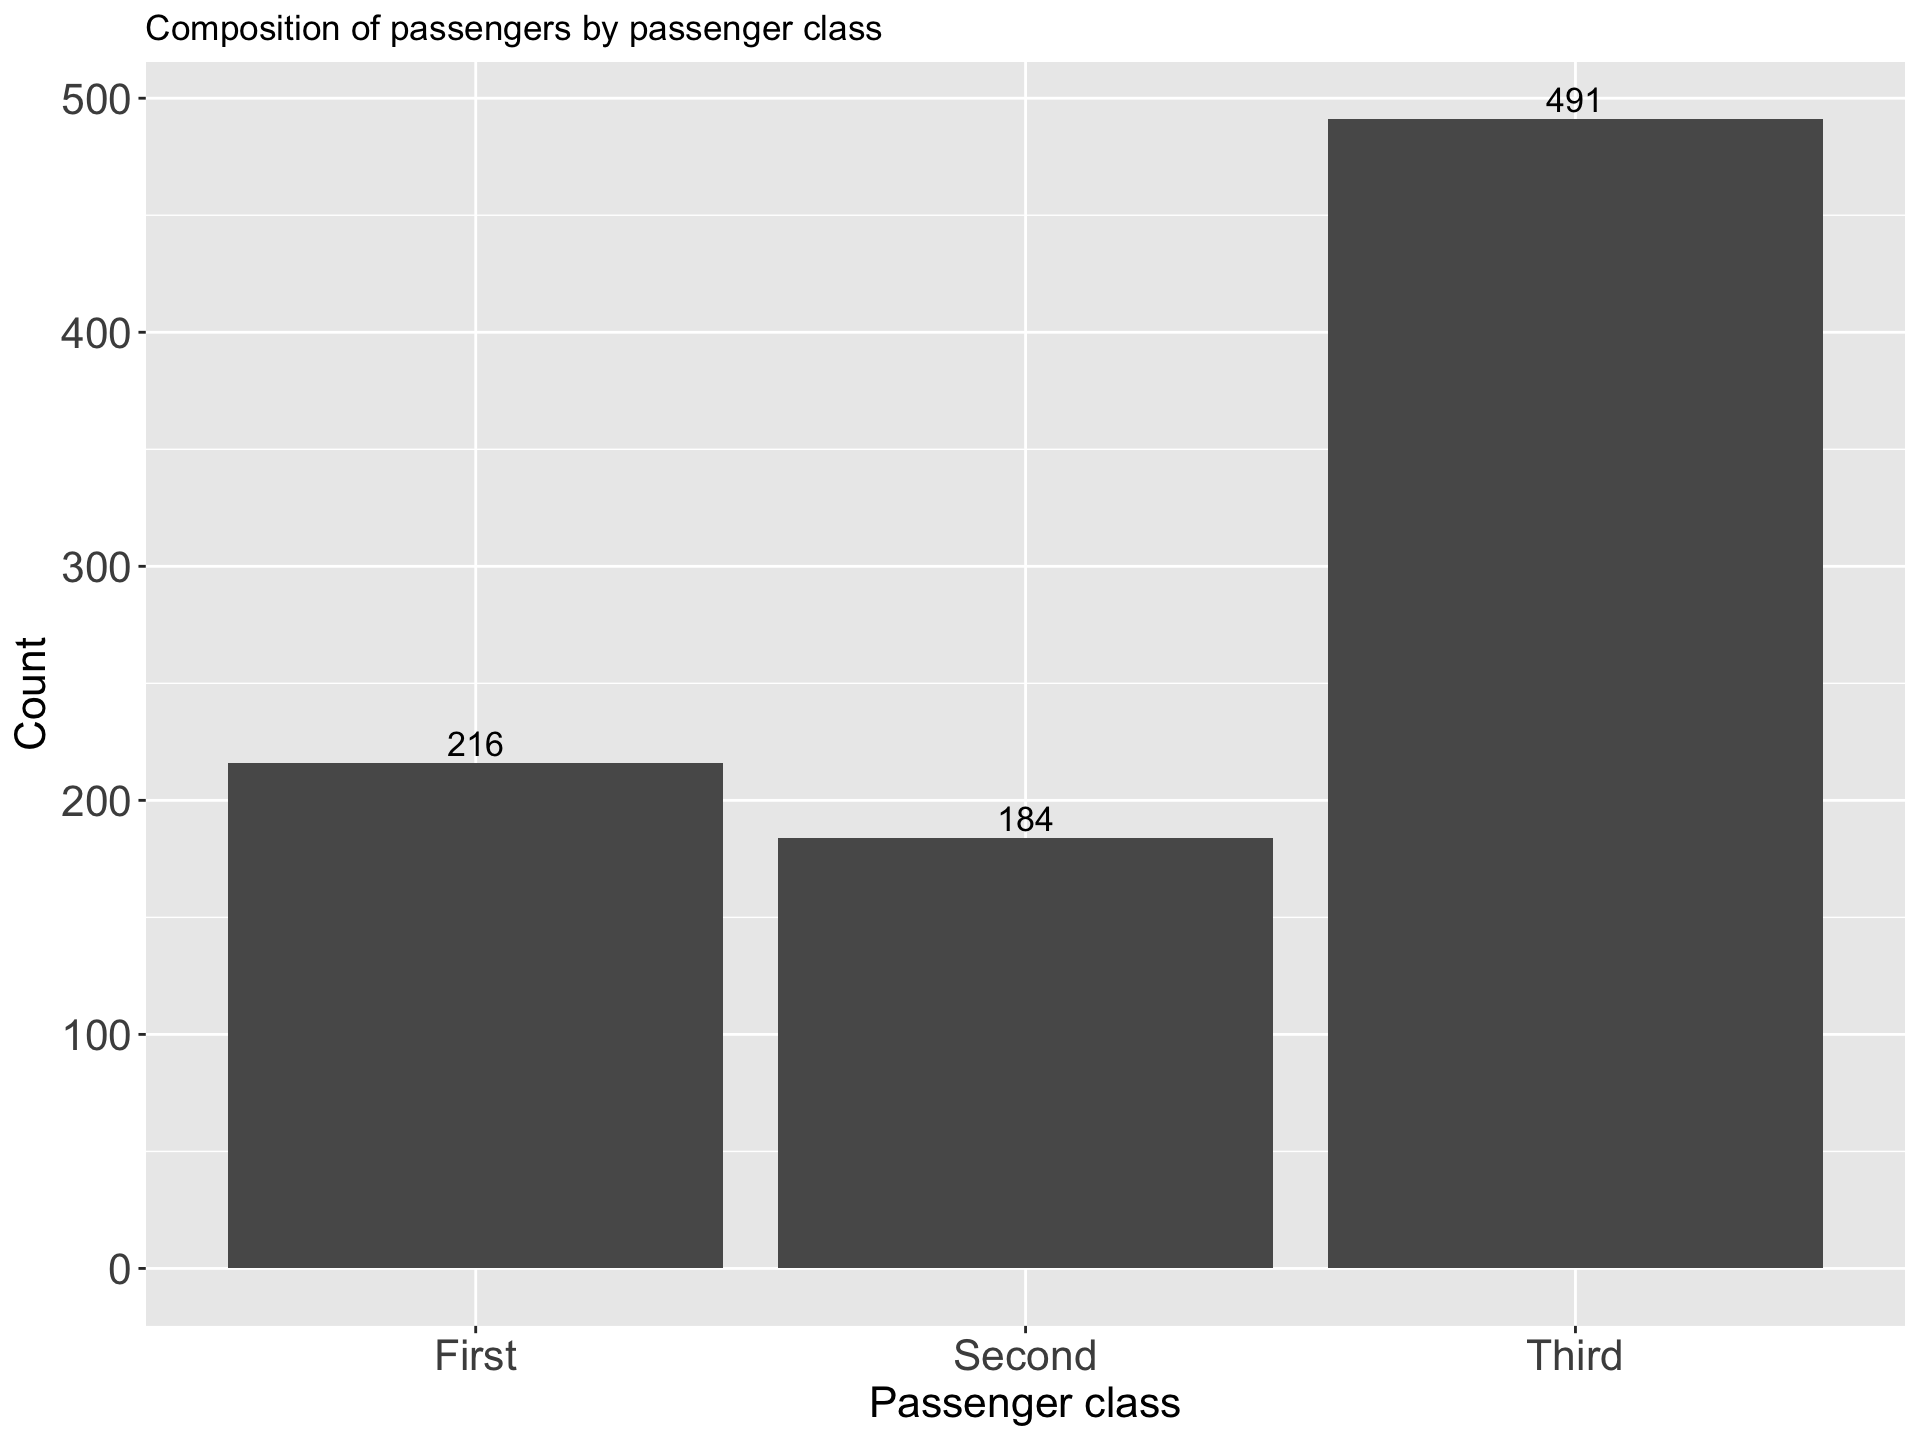
\includegraphics[width=0.8\linewidth]{figure/box8-1} \end{center}

\begin{center}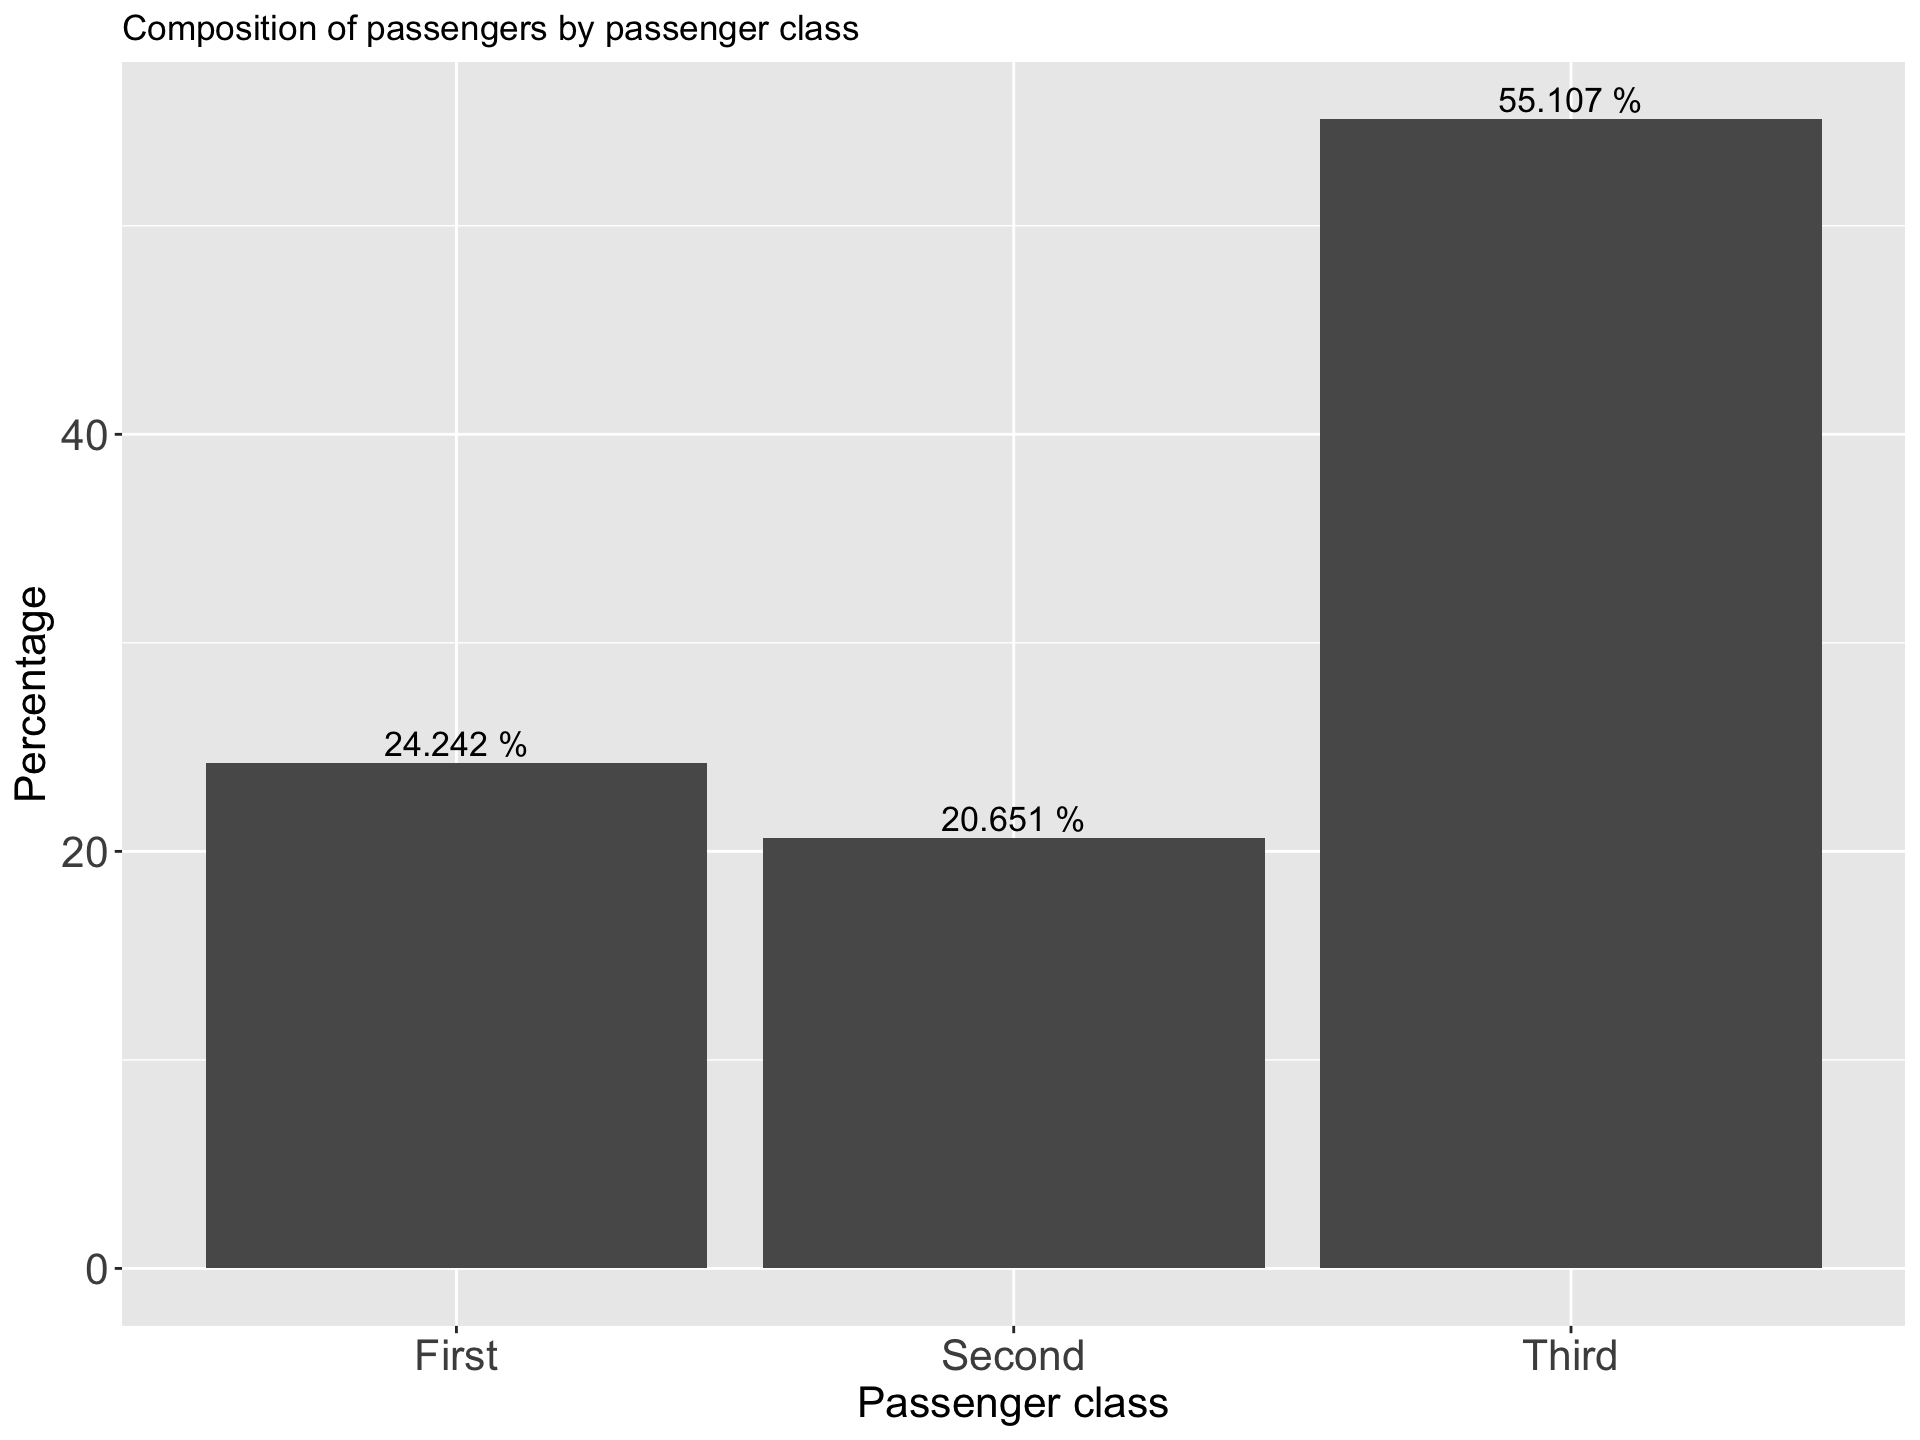
\includegraphics[width=0.8\linewidth]{figure/box9-1} \end{center}

\textbf{ii Component Bar Chart }

\begin{itemize}
\tightlist
\item
  \textbf{Sub divided bar chart/ Stacked bar chart}
\item
  Use to compare two or more qualitative variables (nominal or ordinal)
\item
  Often used in conjunction with two way tables
\item
  Start by drawing a simple bar chart with the total figures.
\item
  The bars are then divided into the component parts
\item
  Can be drawn on absolute figures or percentages
\item
  The various components should be kept in the same order in each bar
\item
  To distinguish different components from one another, different colours or shades can be used
\end{itemize}

\begin{tabular}{l|r|r|r}
\hline
Survived & First & Second & Third\\
\hline
died & 80 & 97 & 372\\
\hline
Survived & 136 & 87 & 119\\
\hline
\end{tabular}

\begin{center}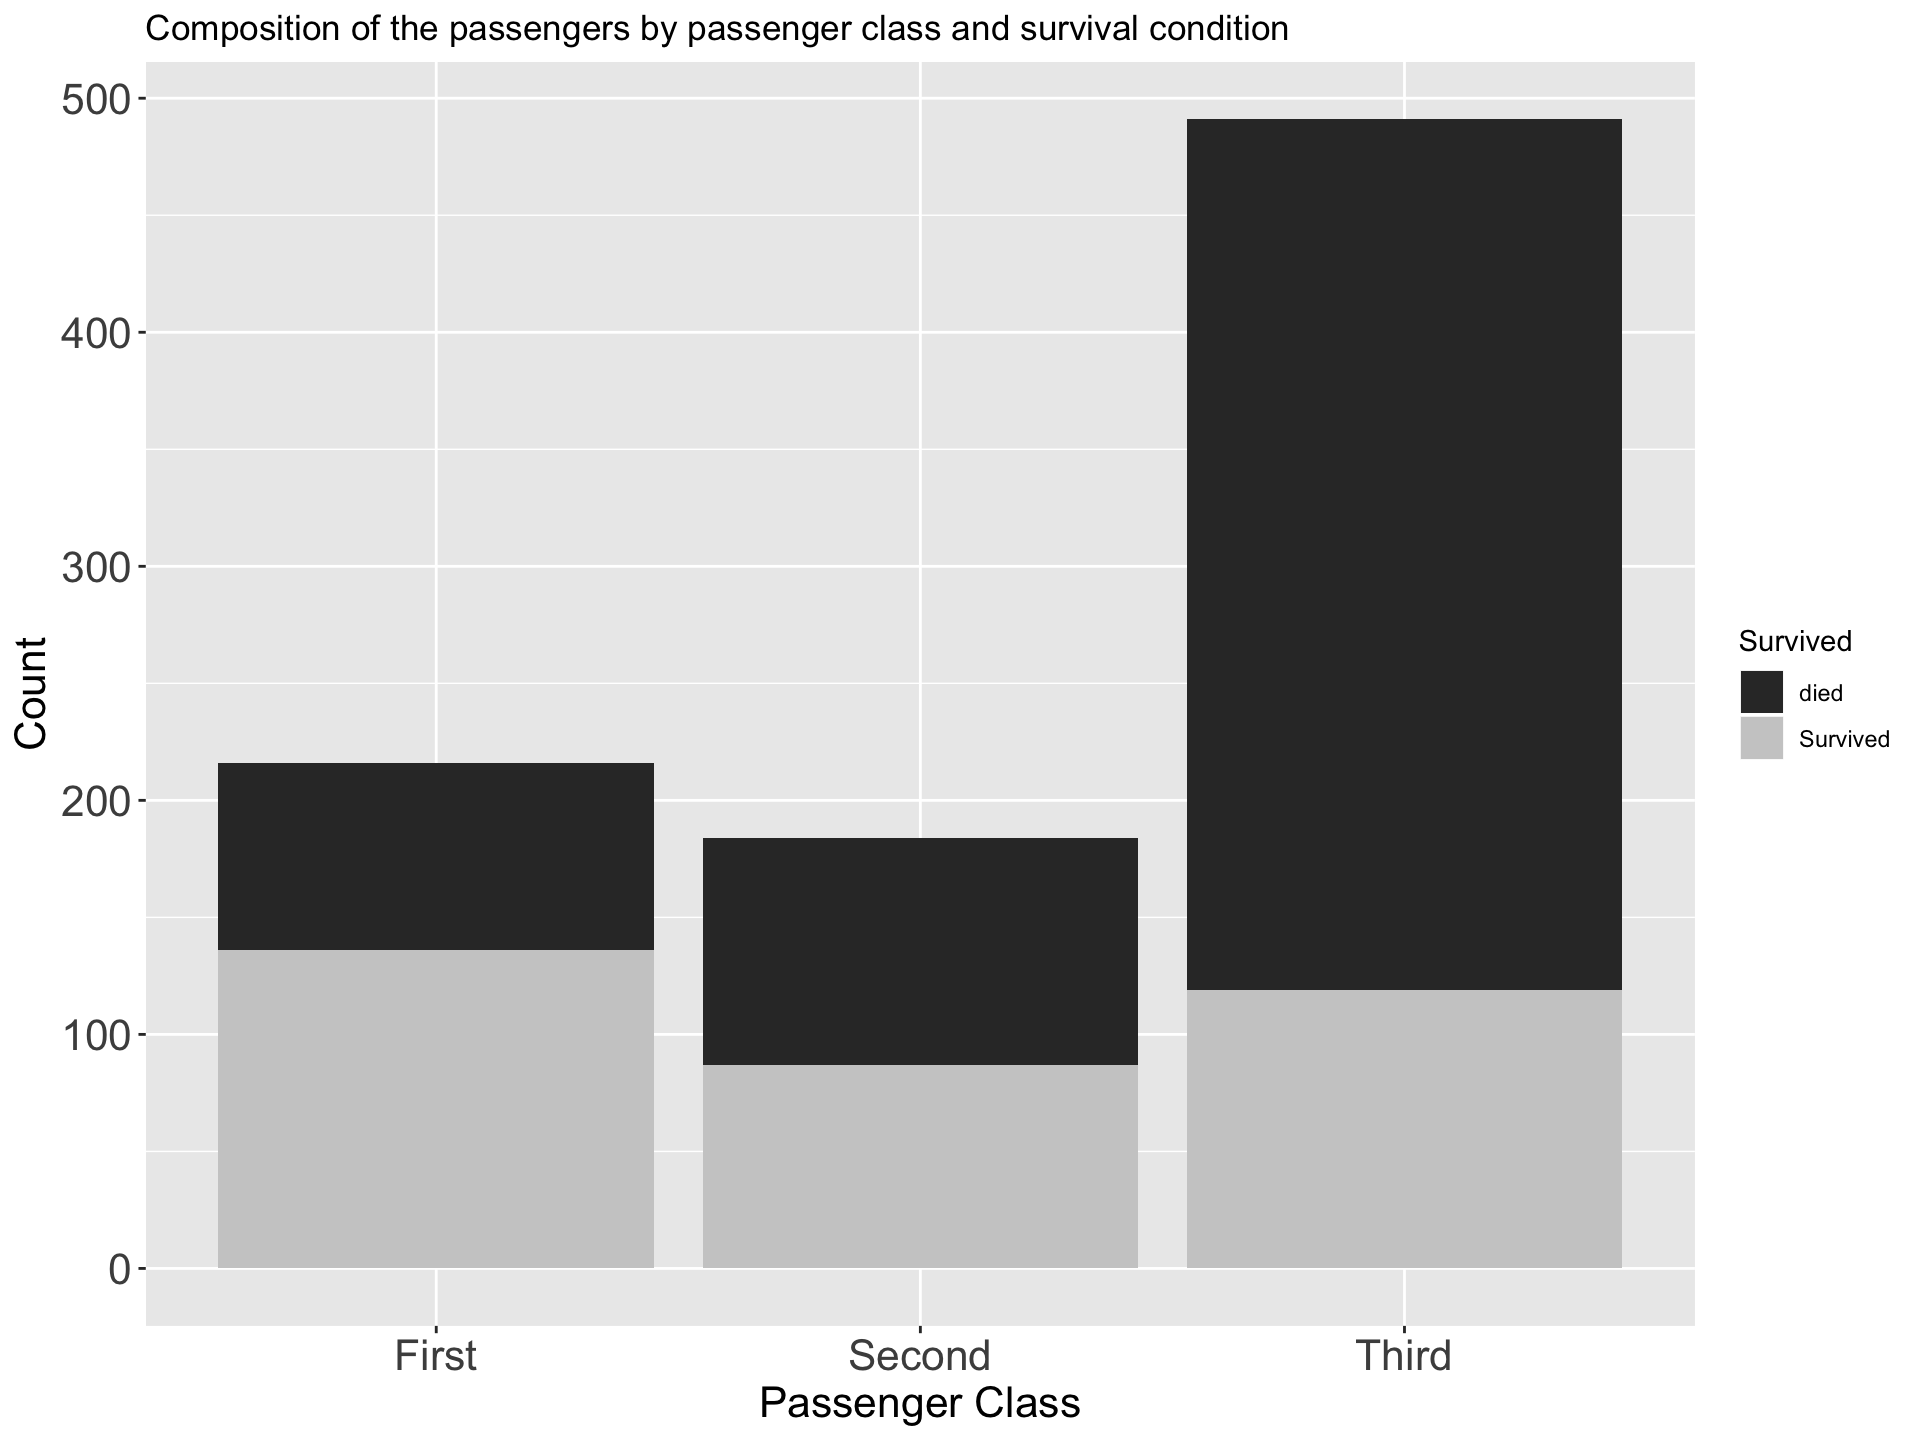
\includegraphics[width=0.8\linewidth]{figure/box10-1} \end{center}

\textbf{Percentage component bar chart}

\begin{itemize}
\tightlist
\item
  When sub-divided bar chart is drawn on percentage basis it is called percentage bar chart
\item
  The various components are expressed as percentage to the total
\item
  All bars are equal in height
\end{itemize}

\begin{tabular}{l|r|r|r}
\hline
Survived & First & Second & Third\\
\hline
died & 0.3703704 & 0.5271739 & 0.7576375\\
\hline
Survived & 0.6296296 & 0.4728261 & 0.2423625\\
\hline
\end{tabular}

\begin{center}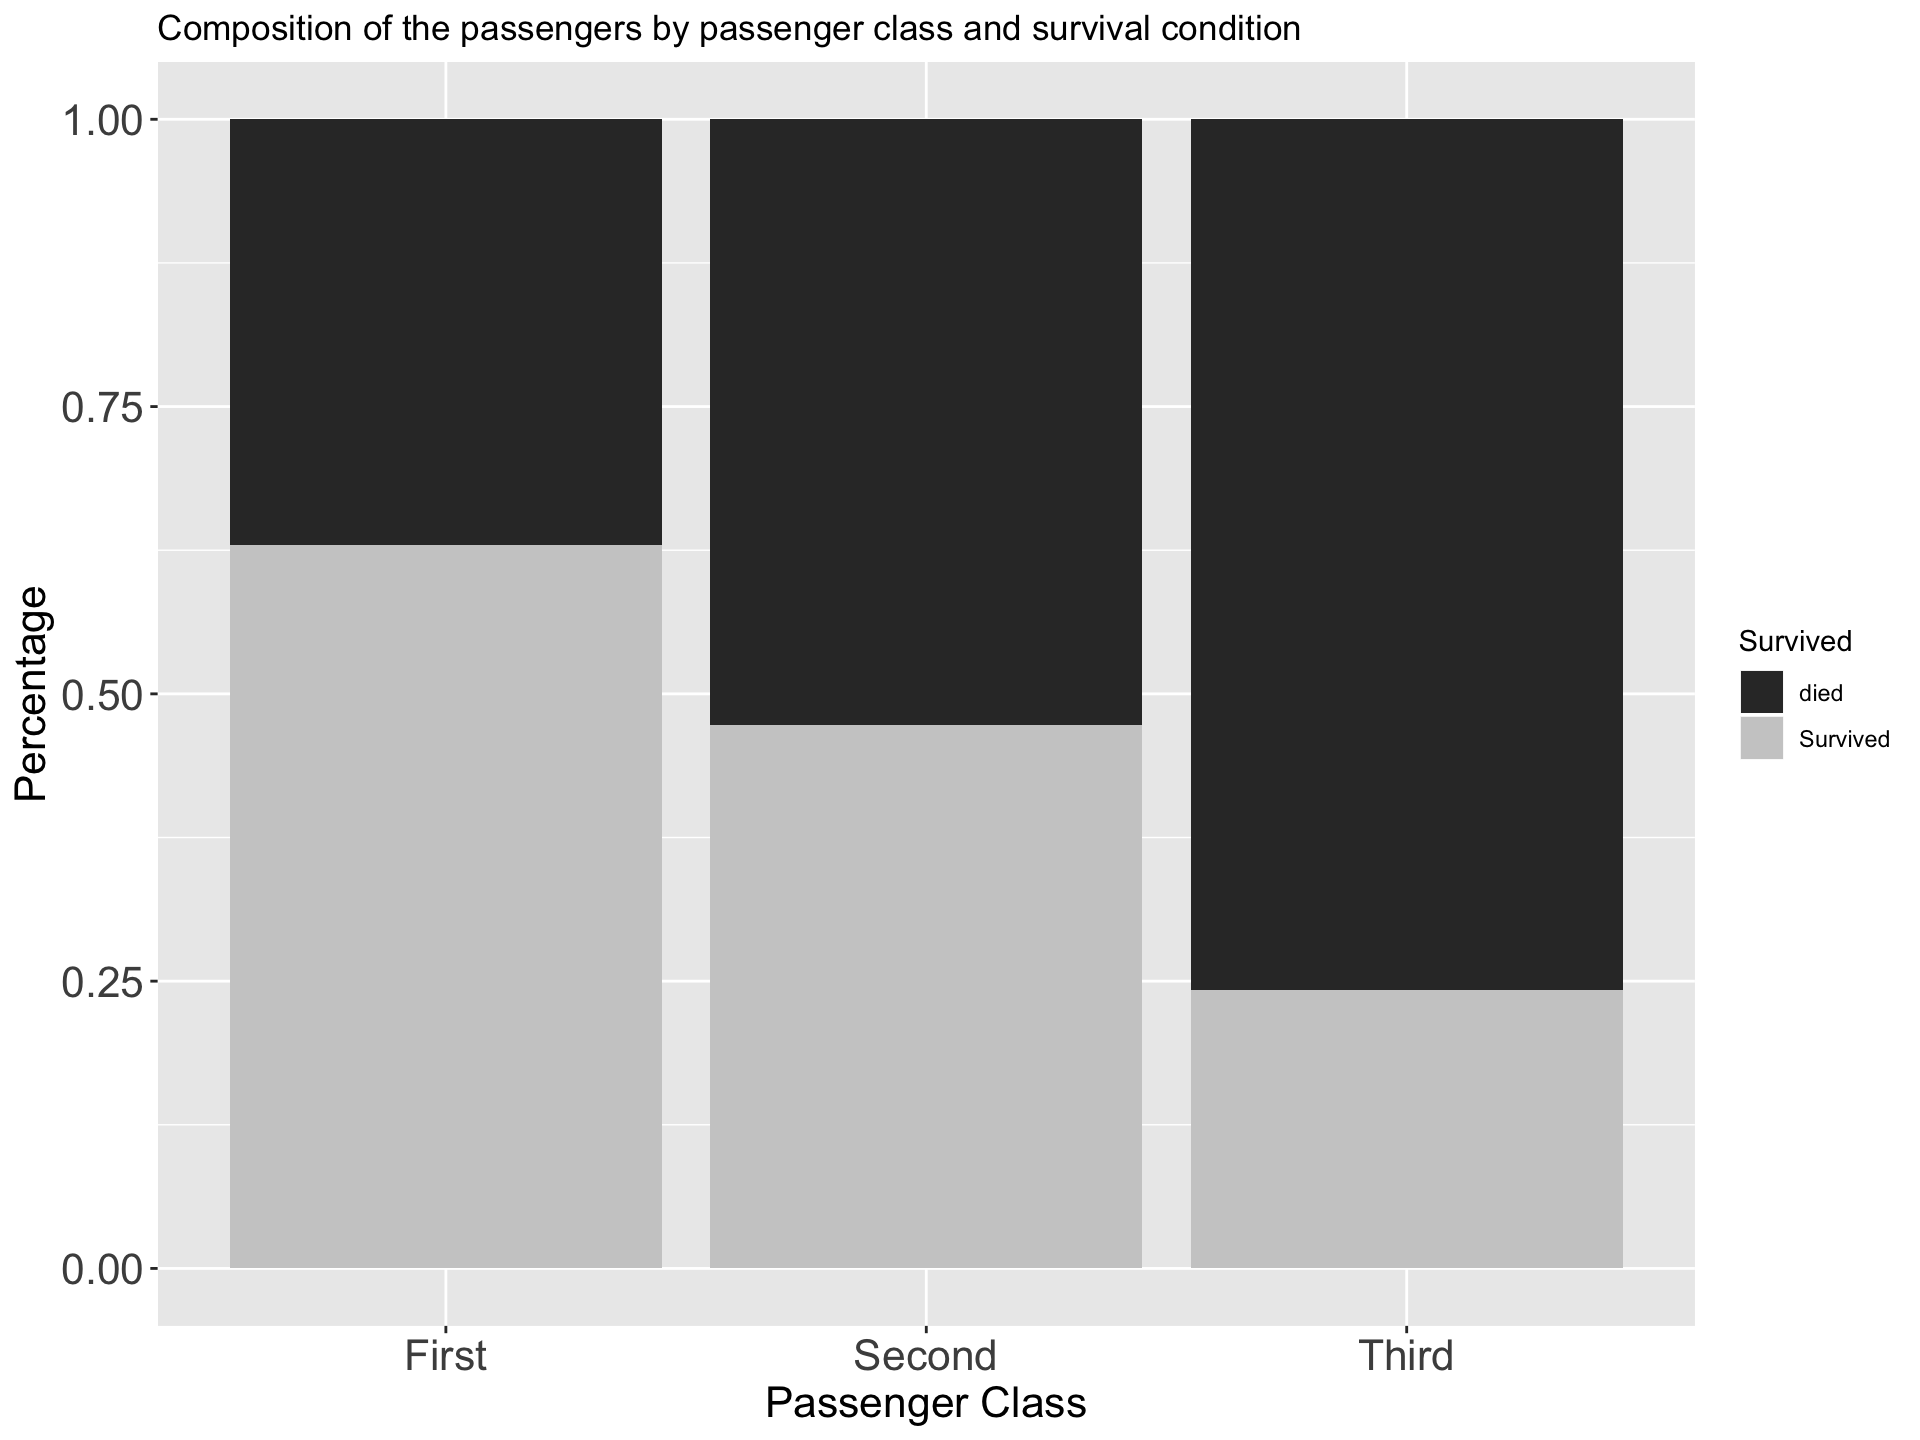
\includegraphics[width=0.8\linewidth]{figure/box11-1} \end{center}

\textbf{iii Multiple Bar Chart}

\begin{itemize}
\tightlist
\item
  Compound bar chart/ Cluster bar chart
\item
  Use to compare two or more qualitative variables (nominal or ordinal)
\item
  Often used in conjunction with two way tables
\item
  These bar charts are drawn side by side
\end{itemize}

\begin{tabular}{l|r|r|r}
\hline
Survived & First & Second & Third\\
\hline
died & 37.04 & 52.72 & 75.76\\
\hline
Survived & 62.96 & 47.28 & 24.24\\
\hline
\end{tabular}

\begin{center}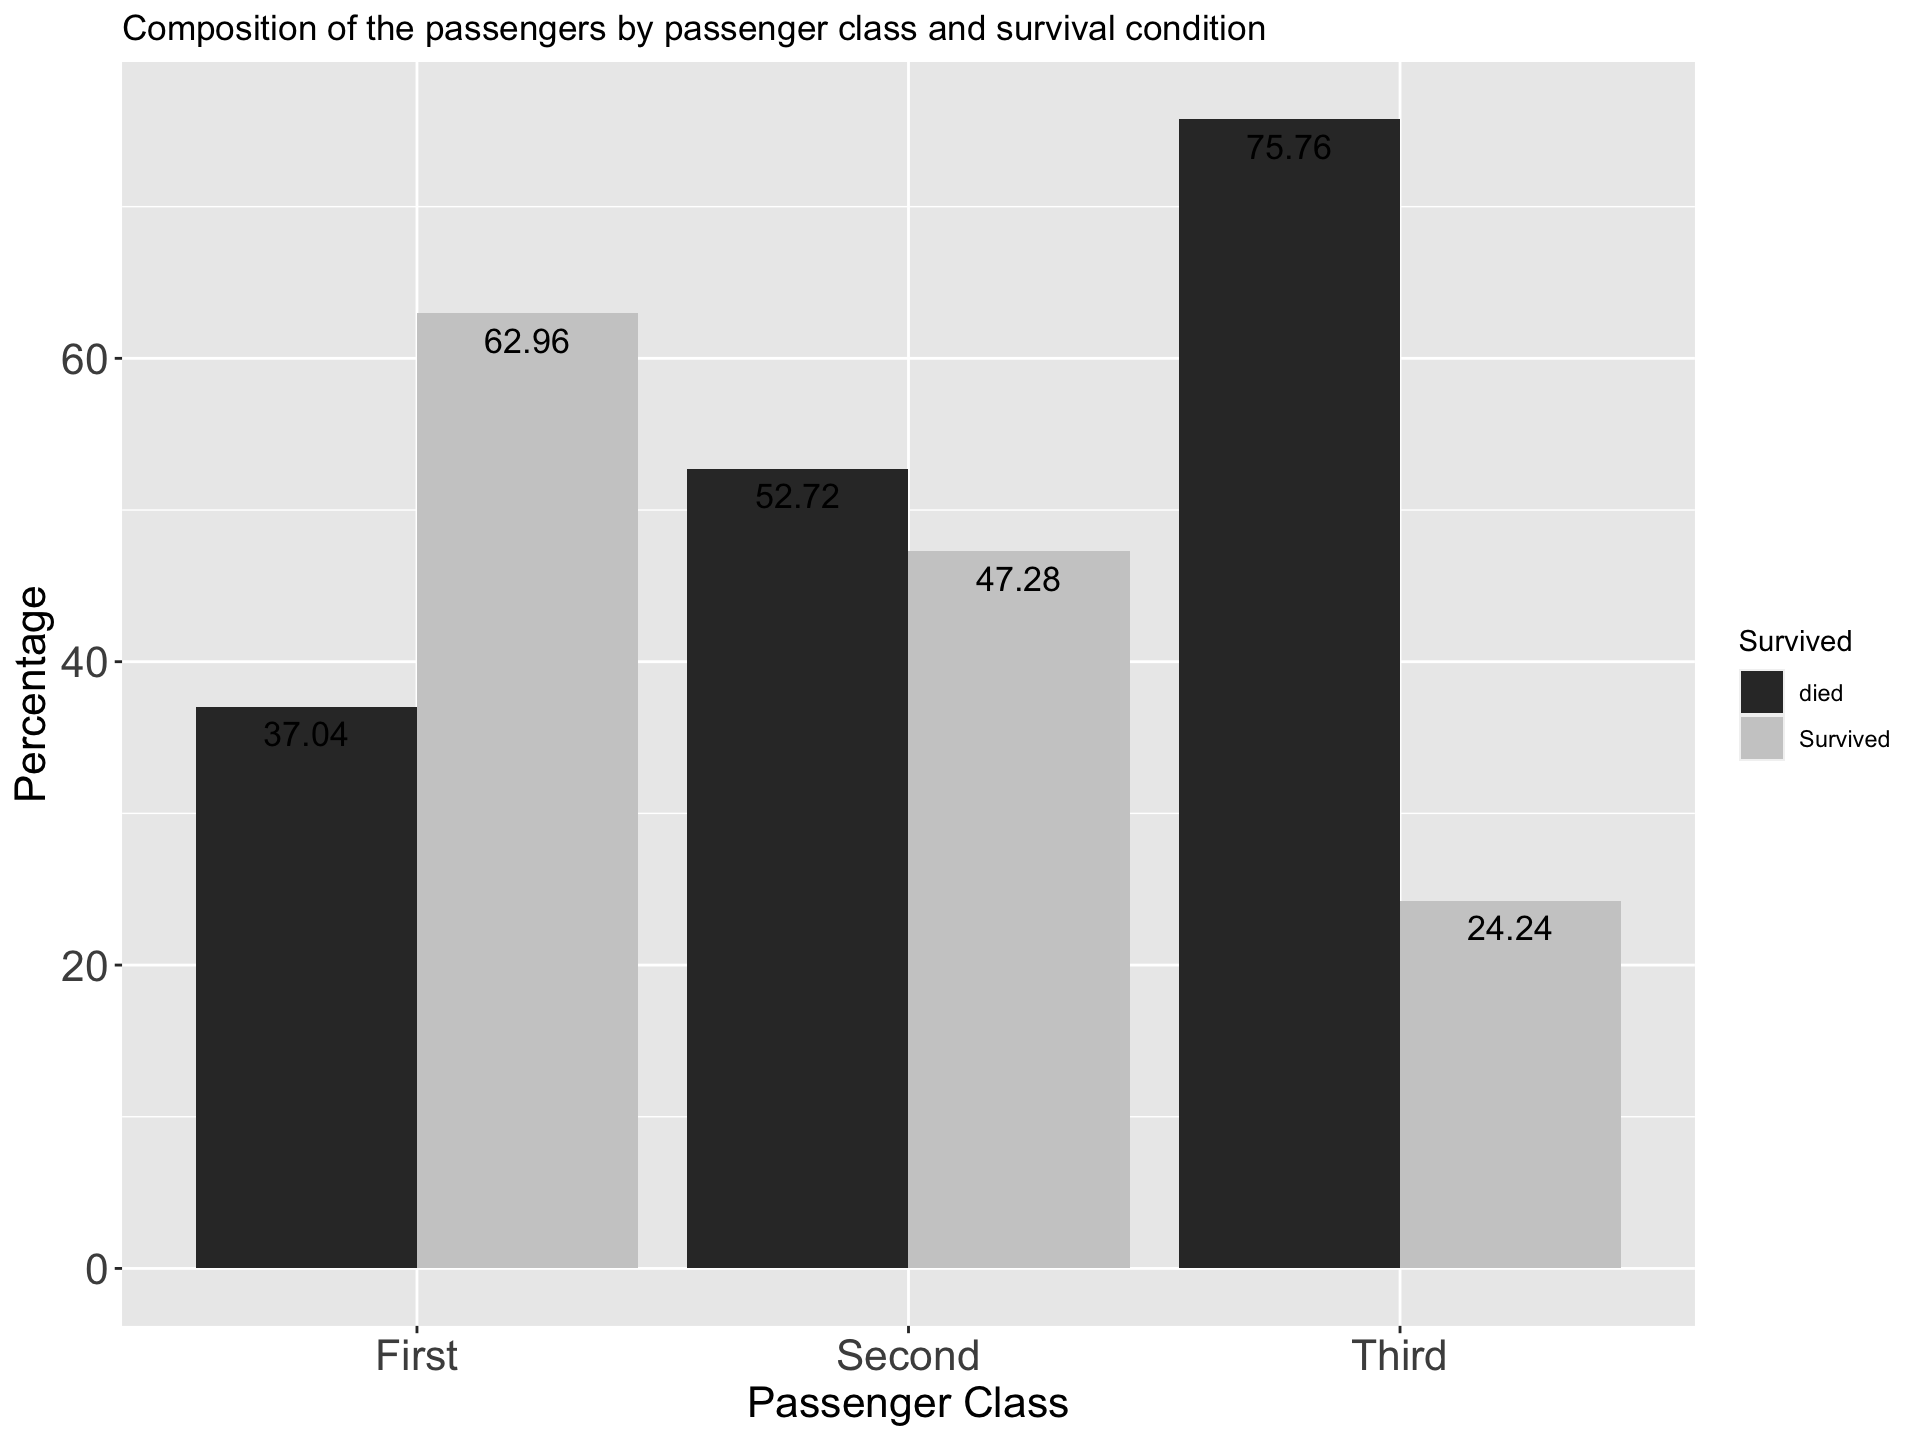
\includegraphics[width=0.8\linewidth]{figure/box12-1} \end{center}

\hypertarget{describing-quantitative-data}{%
\subsubsection{Describing Quantitative Data}\label{describing-quantitative-data}}

\begin{itemize}
\tightlist
\item
  Histogram/ Dot plot / Box plot/ Scatter plot
\end{itemize}

\textbf{II Histogram}

\begin{itemize}
\tightlist
\item
  Histogram looks similar to bar chart since it also has bars.
\item
  However, it is different from a bar chart in a number of aspects.
\item
  One main difference is that in the histogram, the bars are drawn attached to each other; there are no gaps between bars like in a bar chart.
\item
  Histogram is used to show the shape of the distribution of a \textbf{continuous variable}.
\item
  However, the histogram is also used for discrete variables when the data are grouped in to class intervals.
\item
  In a histogram, \textbf{the area of a bar should be proportional to the frequency of the corresponding class.}
\item
  If all the bars have the same width, then the height of a bar can represent the frequency.
\item
  The bar corresponding to a class interval should be drawn from the lower class boundary to the upper class boundary. In this way there will be no gaps between the bars.
\end{itemize}

Example: The marks(out of 50) of a group of students are recorded in the accompanying table. Draw a histogram for the data

\begin{longtable}[]{@{}ll@{}}
\toprule
Marks & Number of students\tabularnewline
\midrule
\endhead
10 - 14 & 4\tabularnewline
15 - 19 & 5\tabularnewline
20 - 24 & 11\tabularnewline
25 - 29 & 9\tabularnewline
30 - 34 & 6\tabularnewline
35 - 39 & 3\tabularnewline
40 - 44 & 2\tabularnewline
Total & 40\tabularnewline
\bottomrule
\end{longtable}

\begin{center}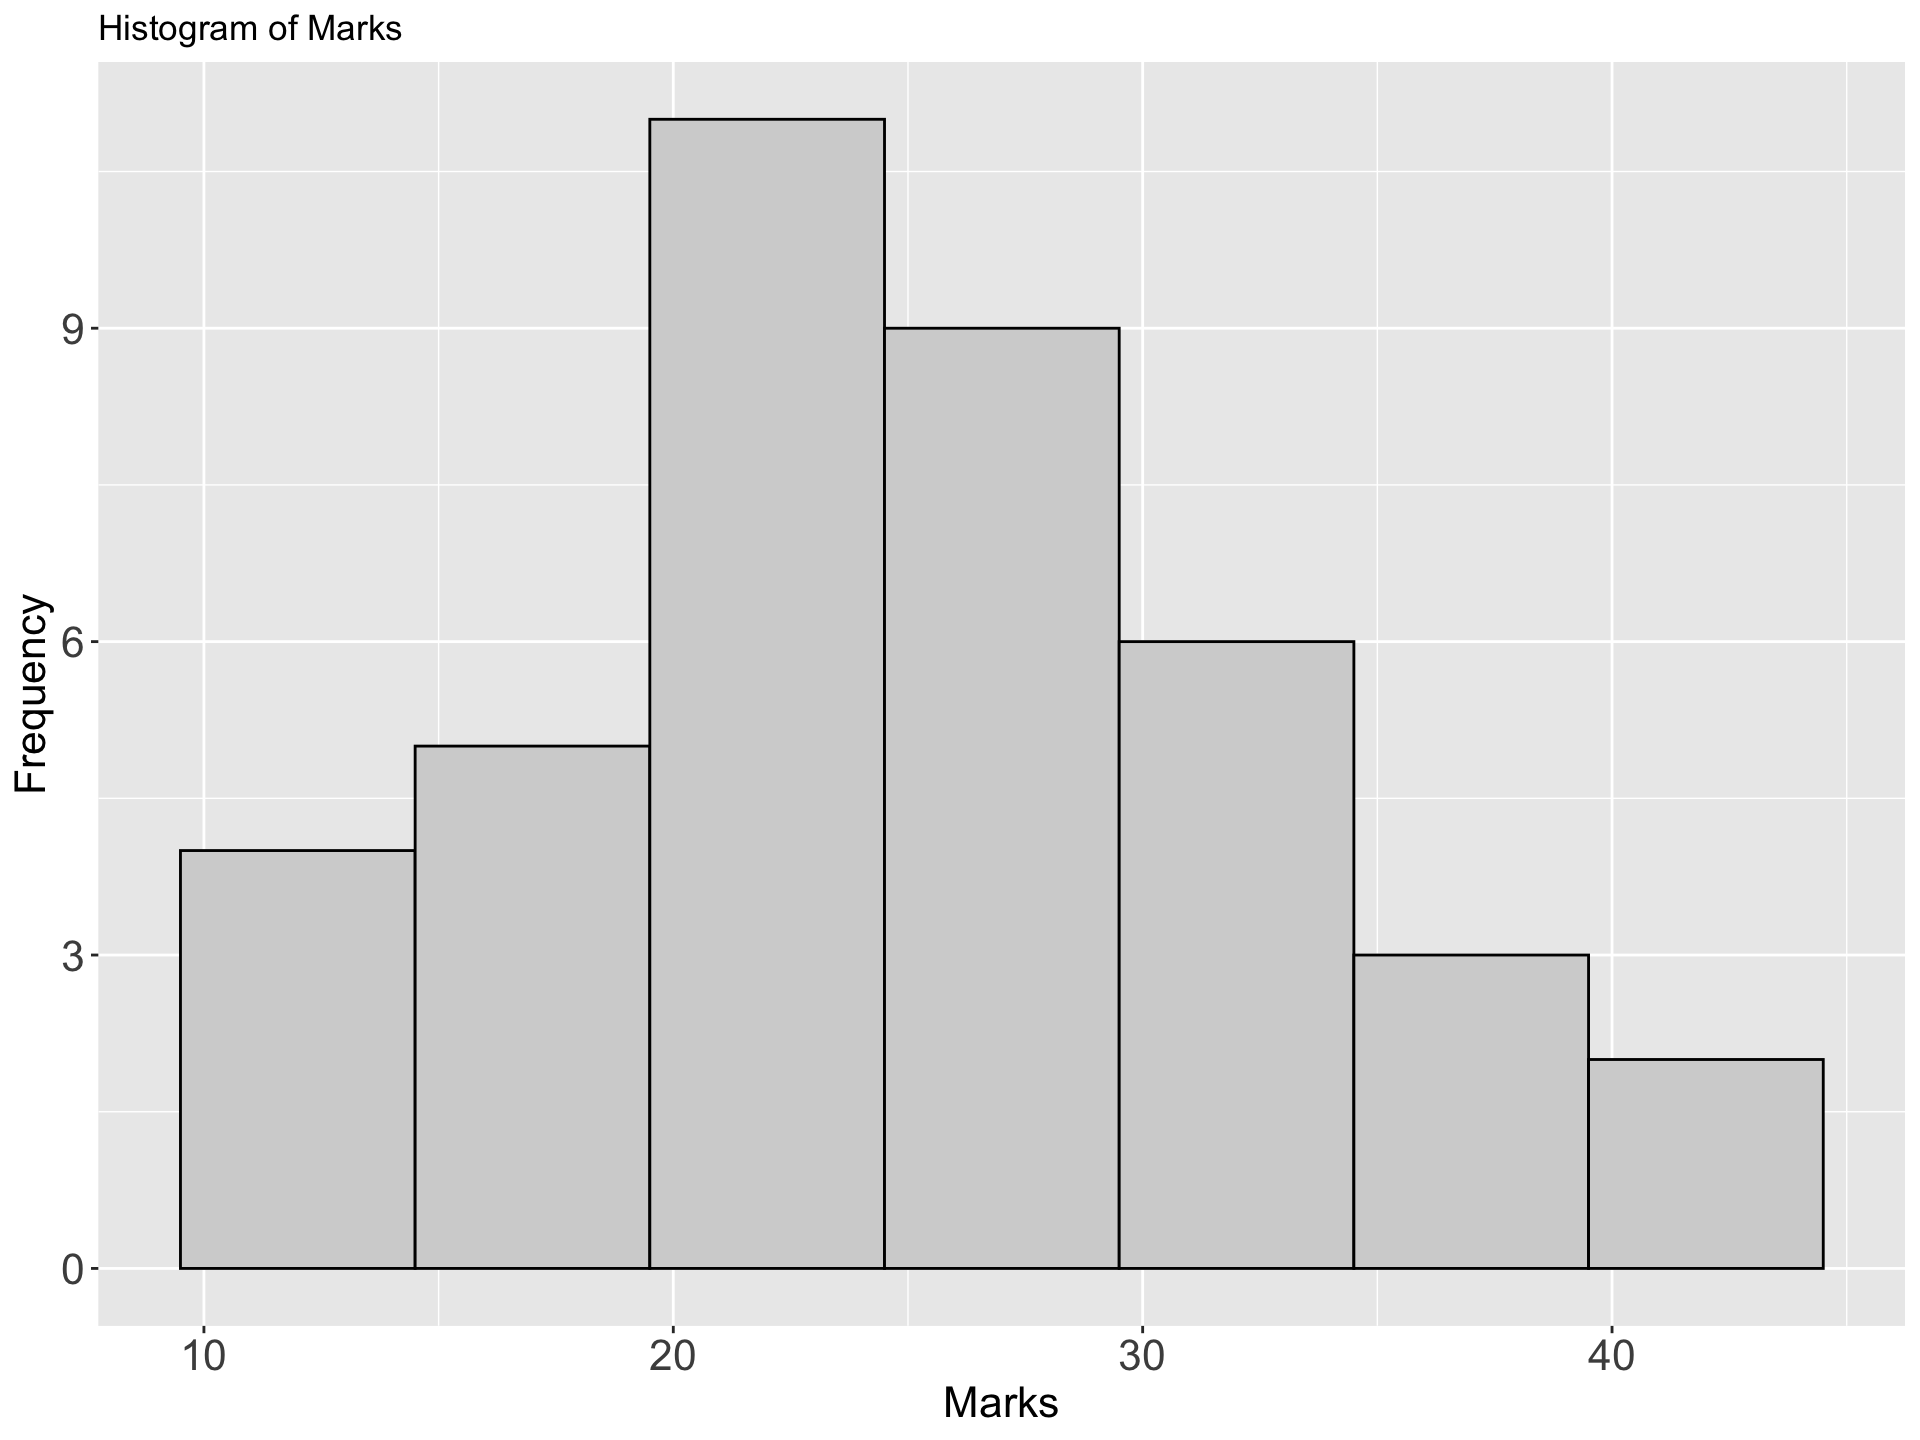
\includegraphics[width=0.8\linewidth]{figure/hist-1} \end{center}

Example 2

\begin{center}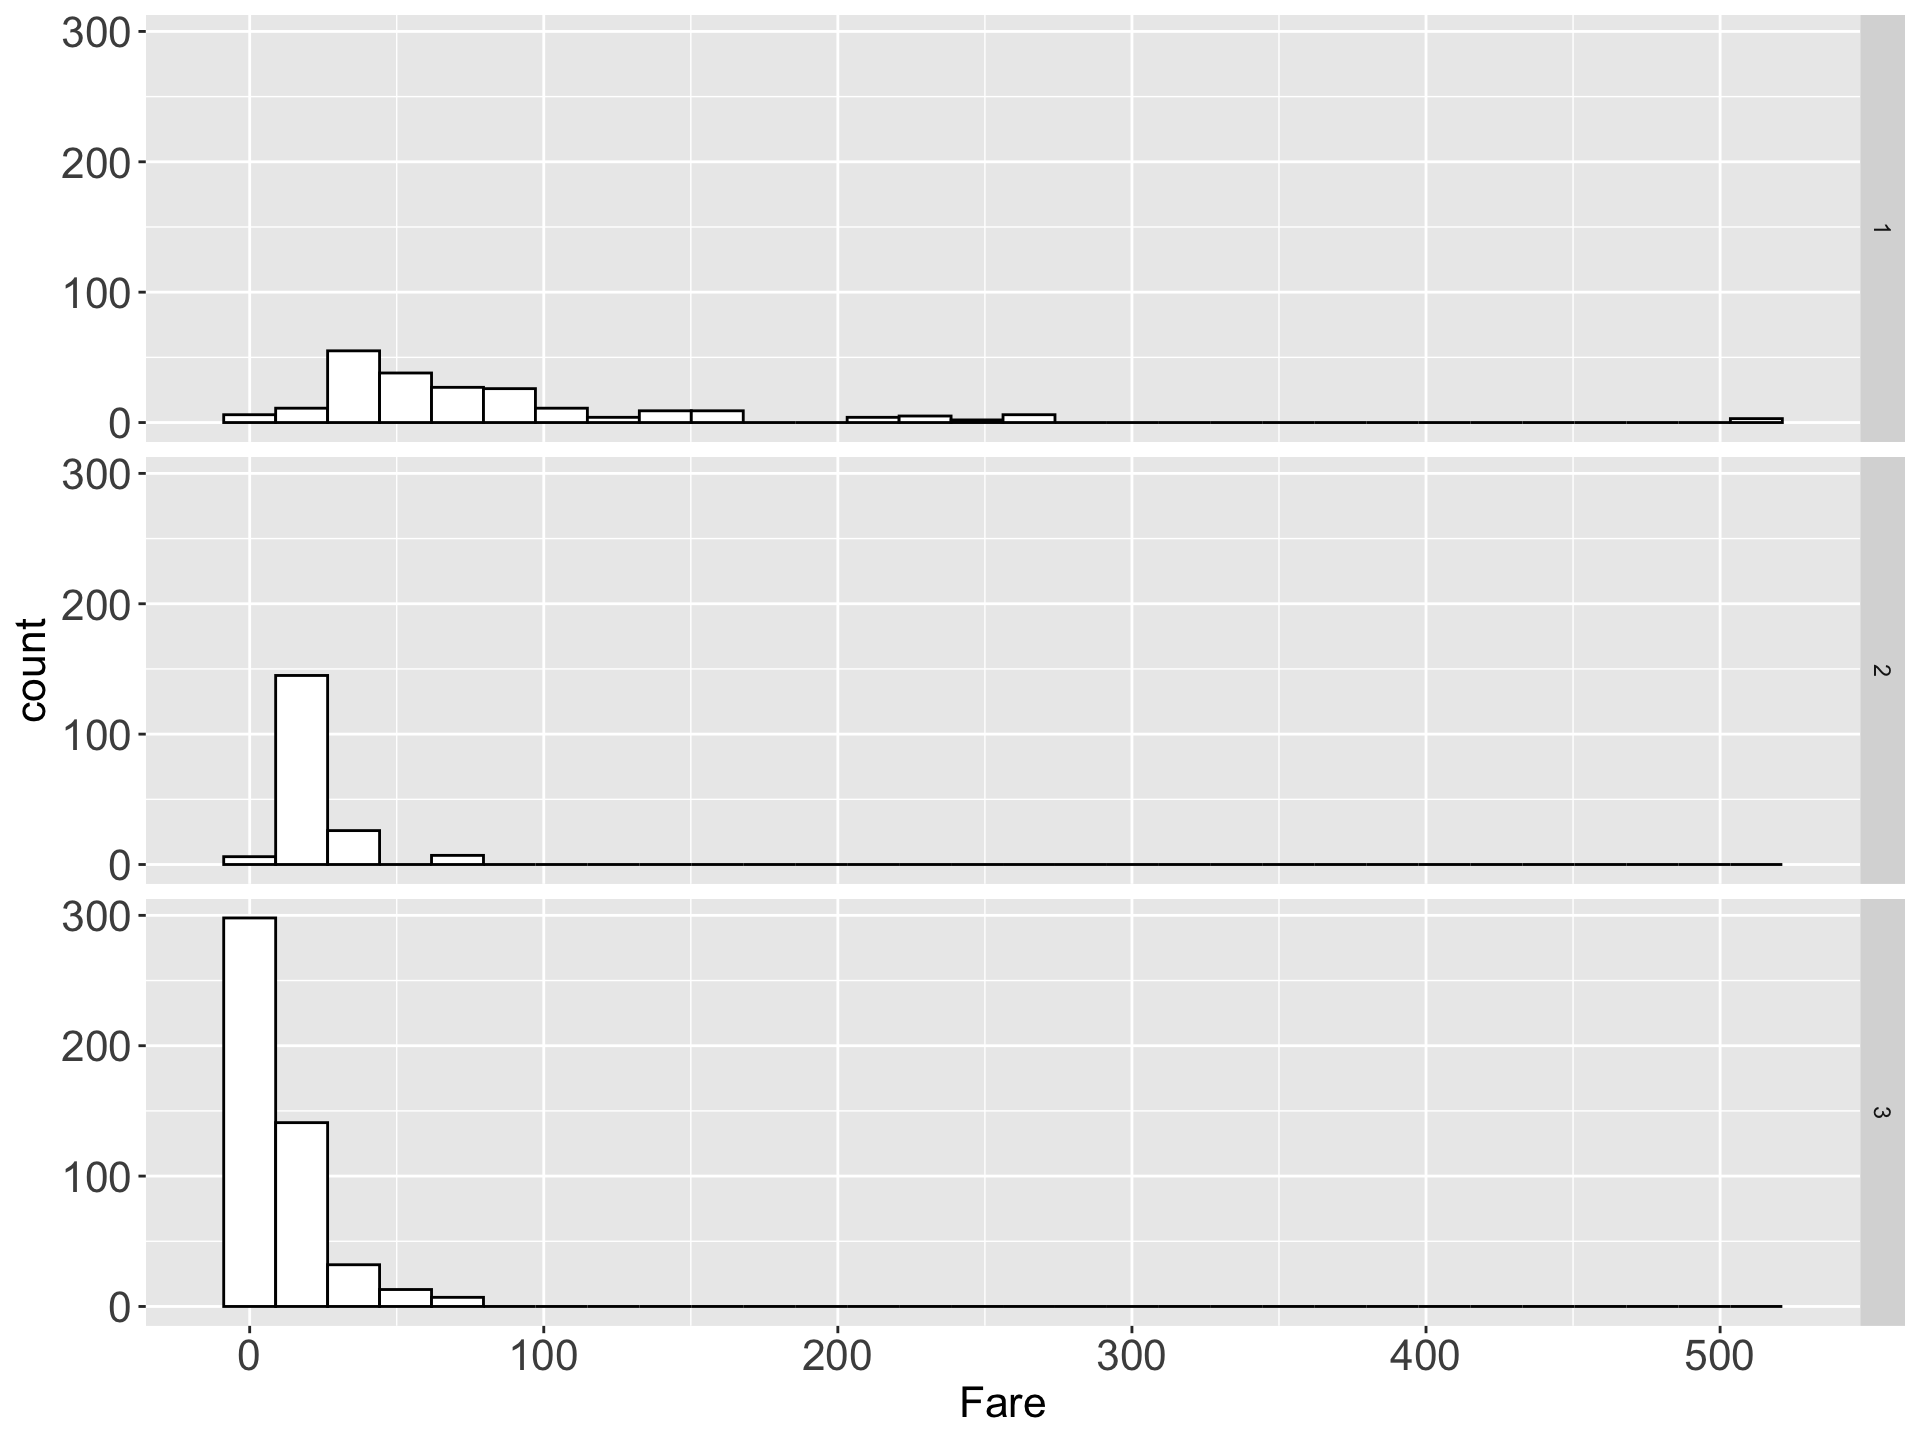
\includegraphics[width=0.8\linewidth]{figure/box18-1} \end{center}

\textbf{III Frequency polygon}

\begin{itemize}
\tightlist
\item
  If the mid-point of the top of each block in a histogram is joined by a straight line, a frequency polygon is produced.
\item
  This is done under the assumption that the frequencies in a class-interval are evenly distributed throughout the class
\end{itemize}

Example: The marks(out of 50) of a group of students are recorded in the accompanying table. Draw a frequency polygon for the data

\begin{longtable}[]{@{}ll@{}}
\toprule
Marks & Number of students\tabularnewline
\midrule
\endhead
10 - 14 & 4\tabularnewline
15 - 19 & 5\tabularnewline
20 - 24 & 11\tabularnewline
25 - 29 & 9\tabularnewline
30 - 34 & 6\tabularnewline
35 - 39 & 3\tabularnewline
40 - 44 & 2\tabularnewline
Total & 40\tabularnewline
\bottomrule
\end{longtable}

\begin{center}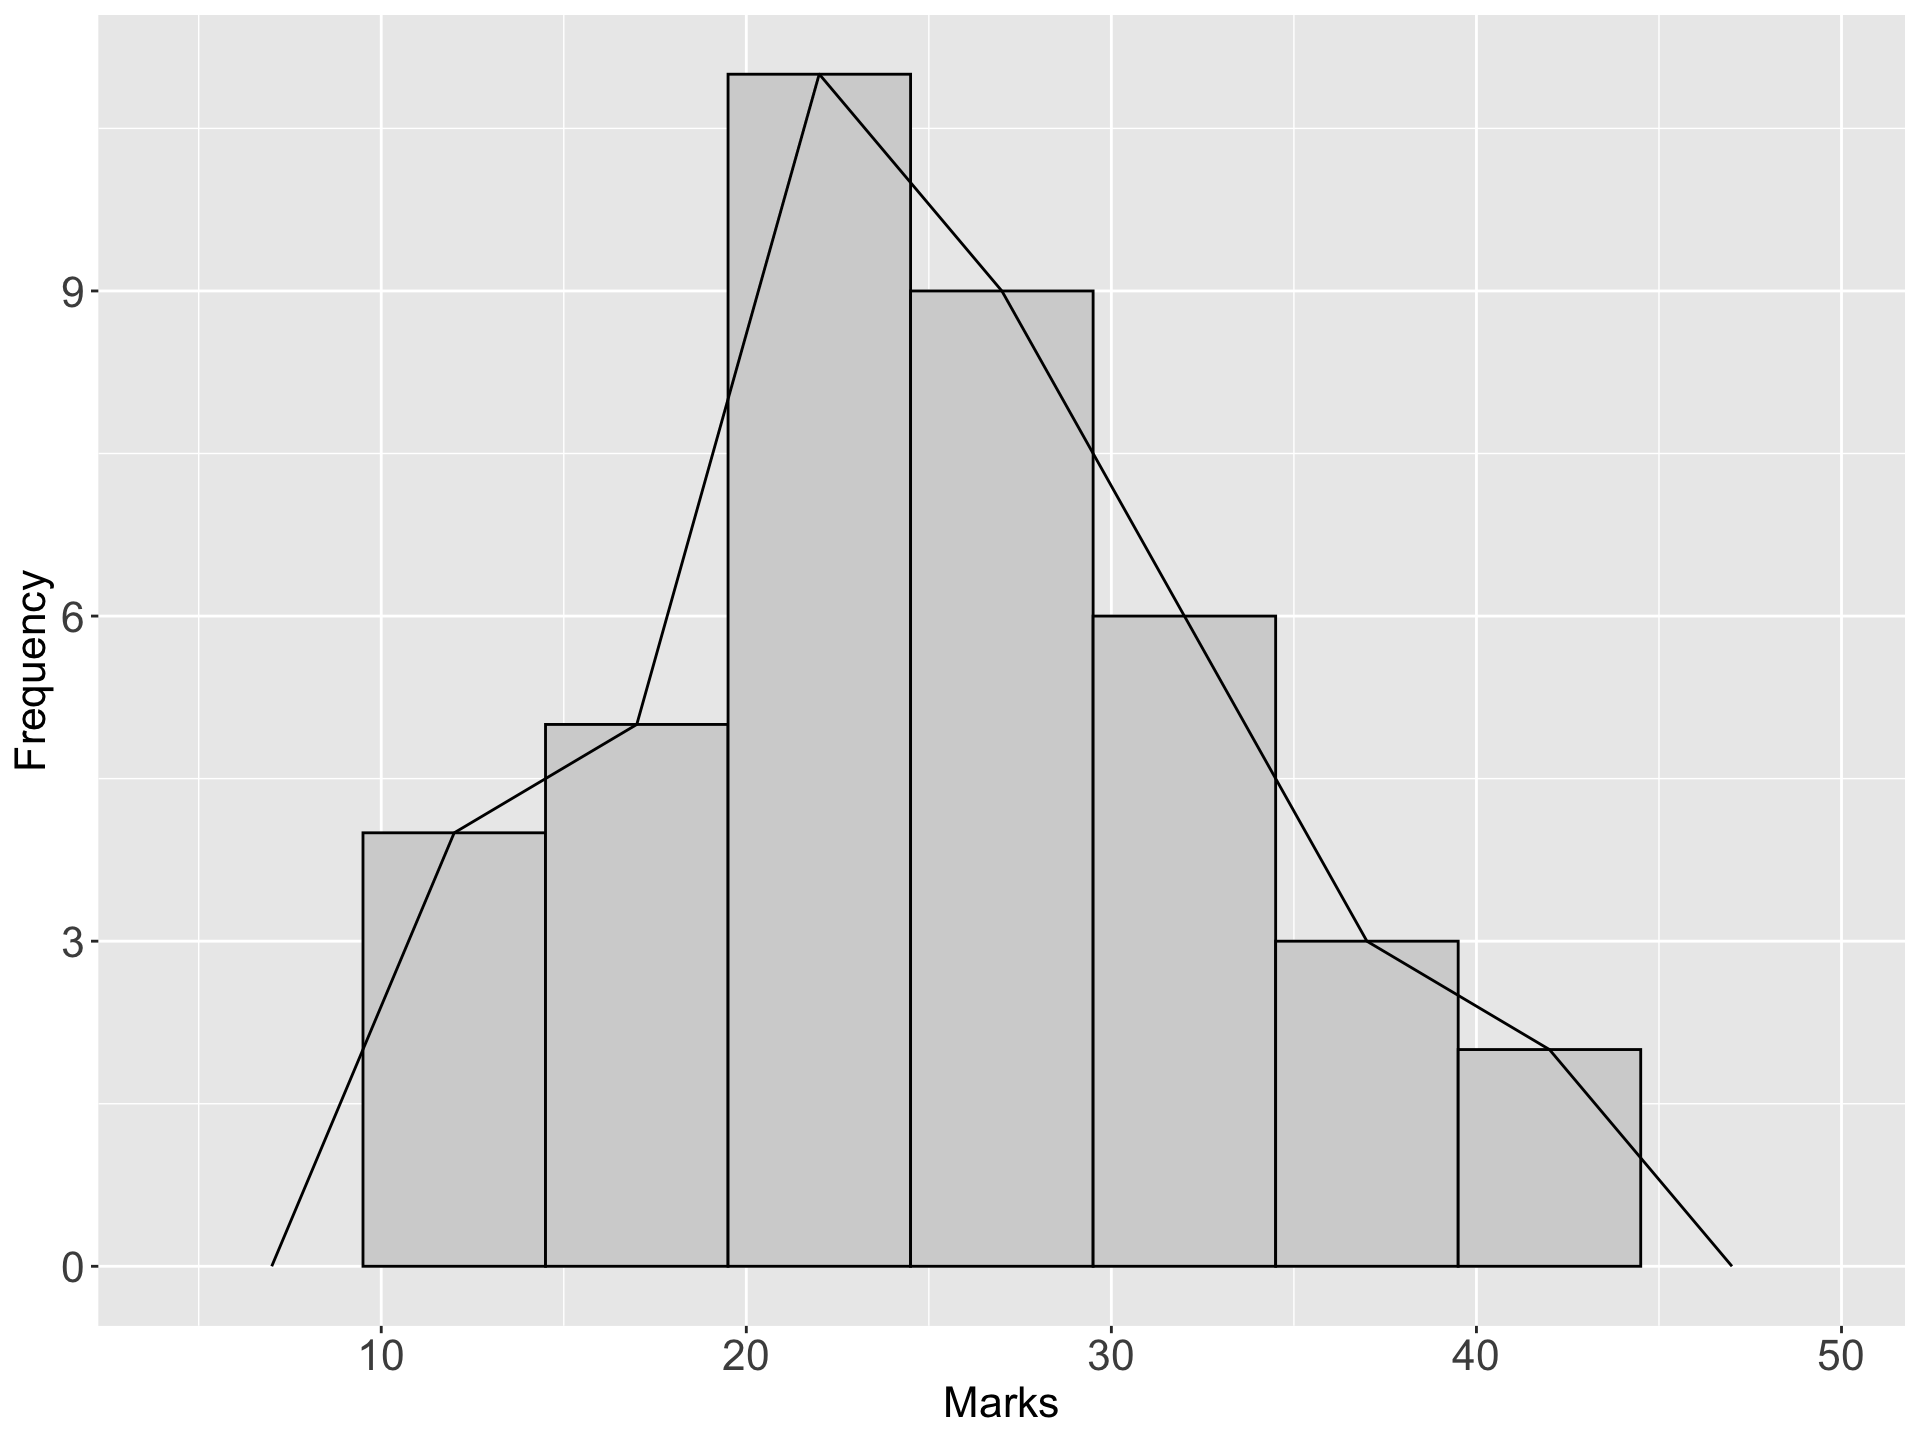
\includegraphics[width=0.8\linewidth]{figure/hist2-1} \end{center}

\textbf{IV Frequency curve}

\begin{itemize}
\tightlist
\item
  A frequency curve is drawn by smoothing the frequency polygon.
\item
  It is smooth in such a way that the sharp turns are avoided
\end{itemize}

Example: The marks(out of 50) of a group of students are recorded in the accompanying table. Draw a frequency curve for the data

\begin{longtable}[]{@{}ll@{}}
\toprule
Marks & Number of students\tabularnewline
\midrule
\endhead
10 - 14 & 4\tabularnewline
15 - 19 & 5\tabularnewline
20 - 24 & 11\tabularnewline
25 - 29 & 9\tabularnewline
30 - 34 & 6\tabularnewline
35 - 39 & 3\tabularnewline
40 - 44 & 2\tabularnewline
Total & 40\tabularnewline
\bottomrule
\end{longtable}

\begin{center}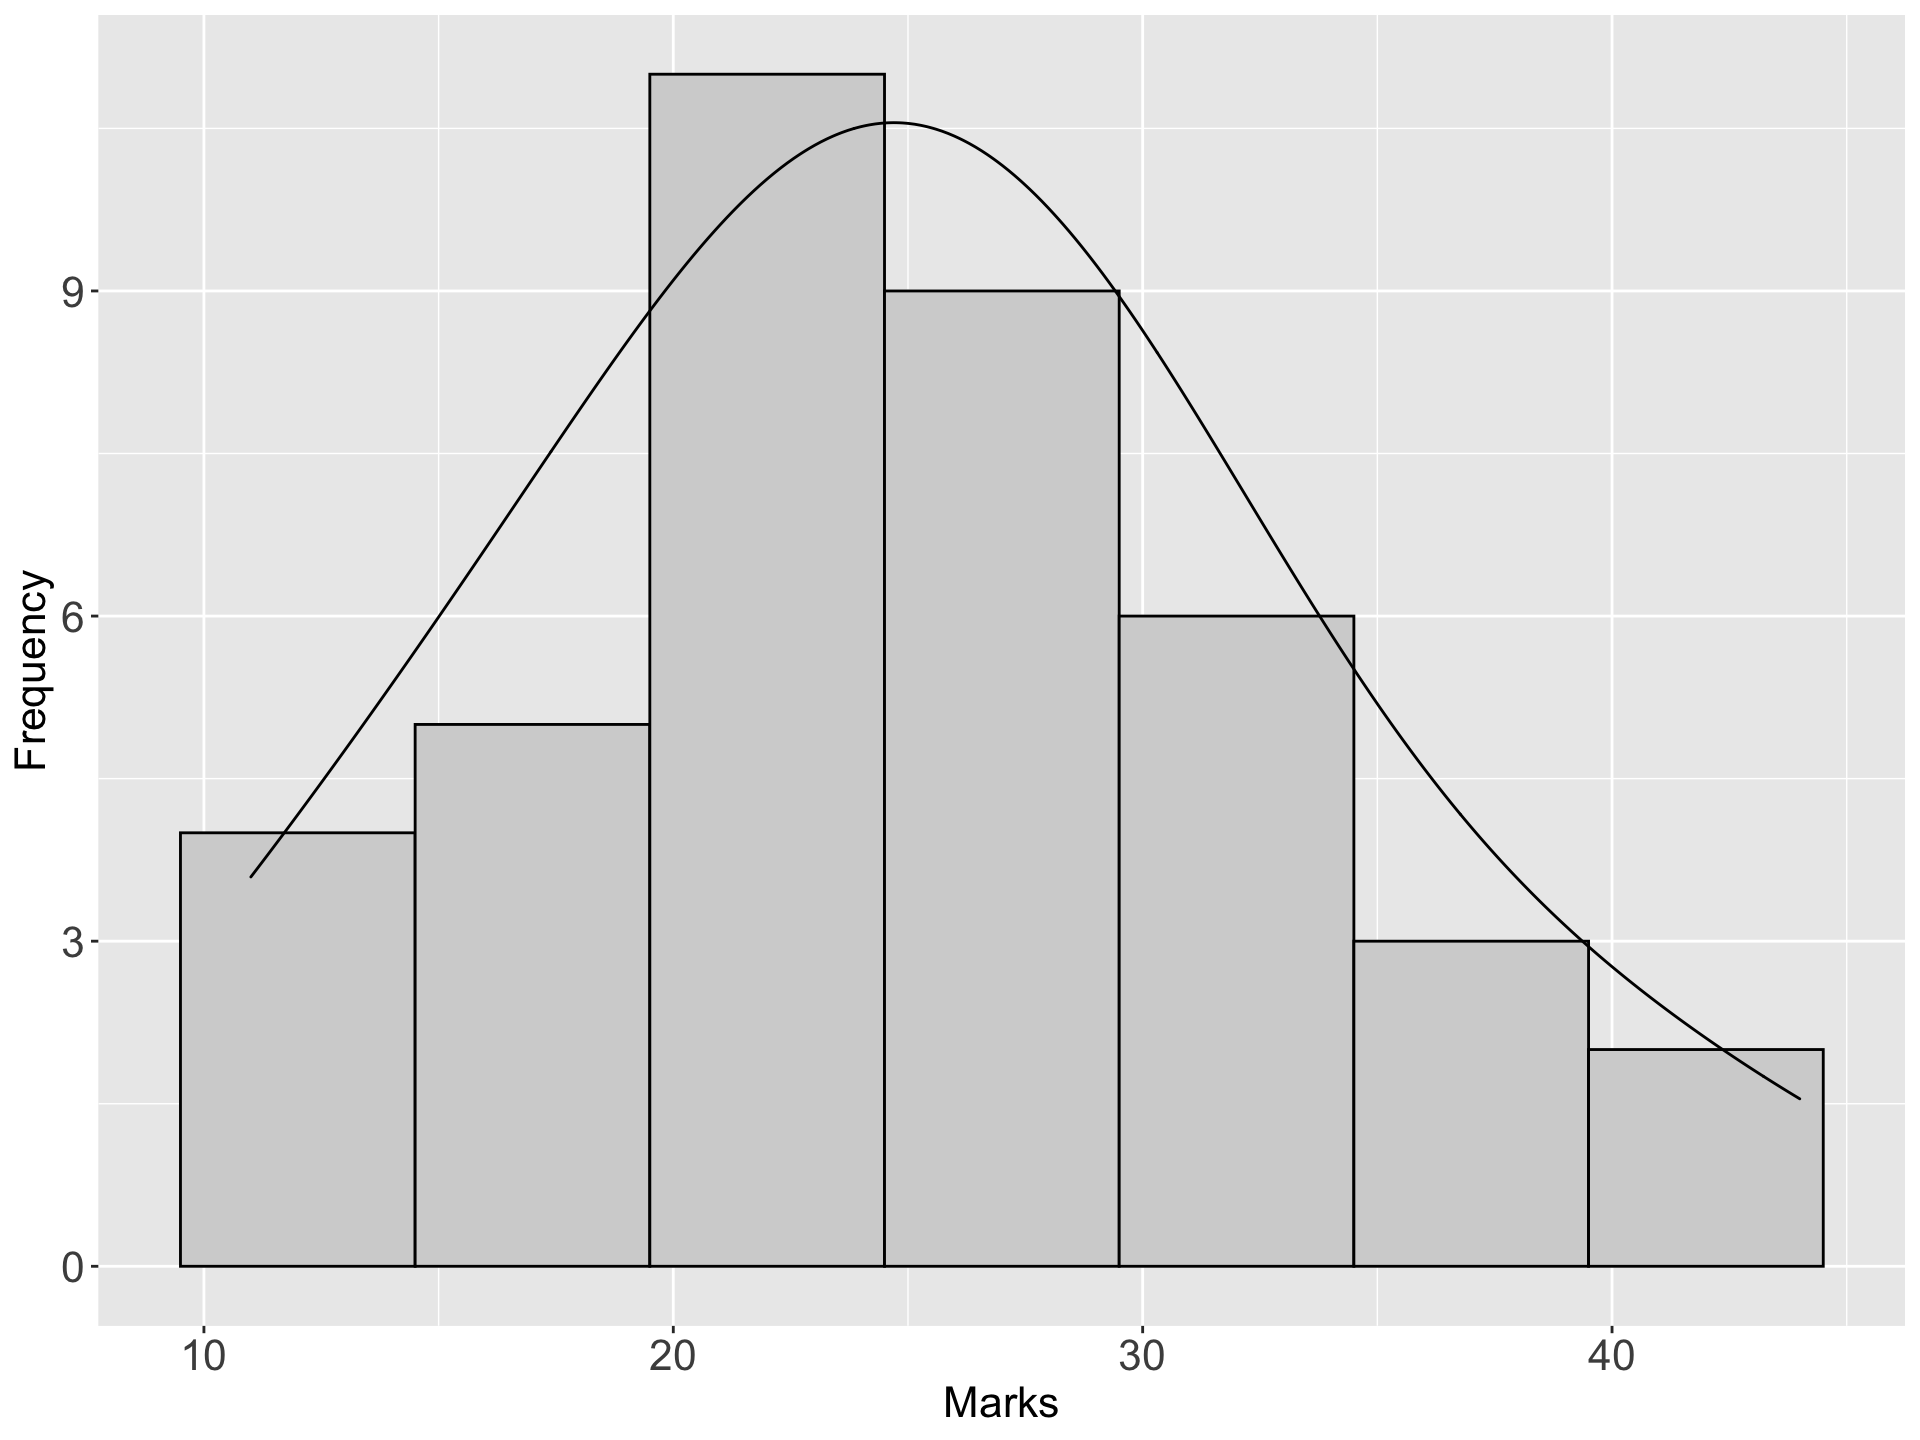
\includegraphics[width=0.8\linewidth]{figure/hist3-1} \end{center}

frequency curves arising in practice take on certain characteristics shapes as shown bellow

\begin{center}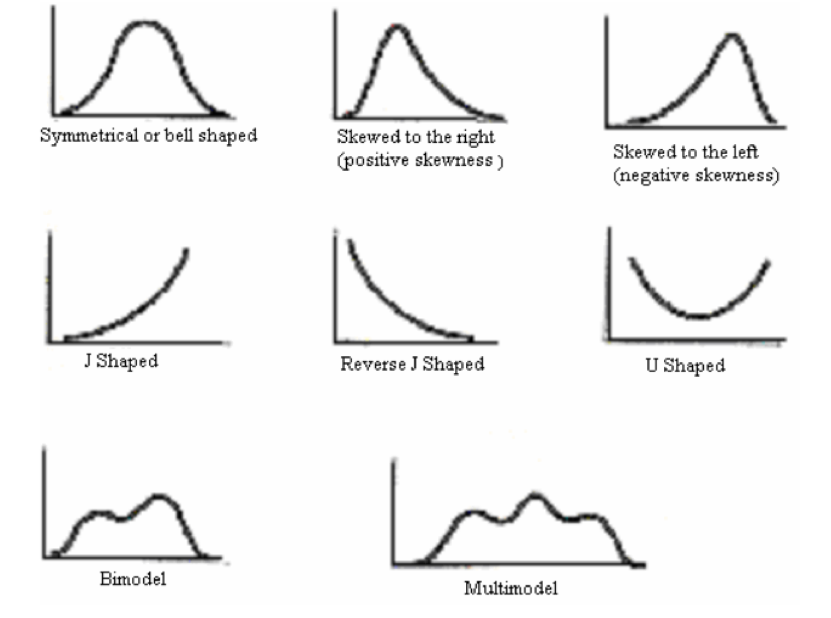
\includegraphics[width=1\linewidth]{figure/shapes} \end{center}

\begin{enumerate}
\def\labelenumi{\arabic{enumi}.}
\tightlist
\item
  The \textbf{symmetrical} or \textbf{bell shaped} frequency curves are characterized by the fact that observations equidistant from the central maximum have the same frequency. An important example is the normal curve.
\item
  In the \textbf{moderately asymmetrical} or \textbf{skewed} frequency curves the tail of the curve to one side of the central maximum is longer than that to the other. If the longer tail occurs to the right the curve is said to be \textbf{skewed to the right} or to have \textbf{positive skewness}.While if the reverse is true the curve is said to be \textbf{skewed to the left} or to have \textbf{negative skewness}.
\item
  In a \textbf{J shaped} or \textbf{reverse J shaped} curve a maximum occurs at one end.
\item
  A \textbf{U shaped} frequency curve has maxima at both ends.
\item
  A \textbf{bimodal} frequency curve has two maxima. These appear as two distinct peaks (local maxima) in the frequency curve.When the two modes are unequal the larger mode is known as the major mode and the other as the minor mode.
\item
  A \textbf{multimodal} frequency curve has more than two maxima.
\end{enumerate}

\textbf{V Dot Plot}

\begin{itemize}
\tightlist
\item
  A dot plot is a method of presenting data which gives a rough but rapid visual appreciation of the way in which the data are distributed
\item
  It consists of a horizontal line marked out with divisions of the scale on which the variable is being measured
  -This graph can be used to represent only the numerical data.
\end{itemize}

\begin{center}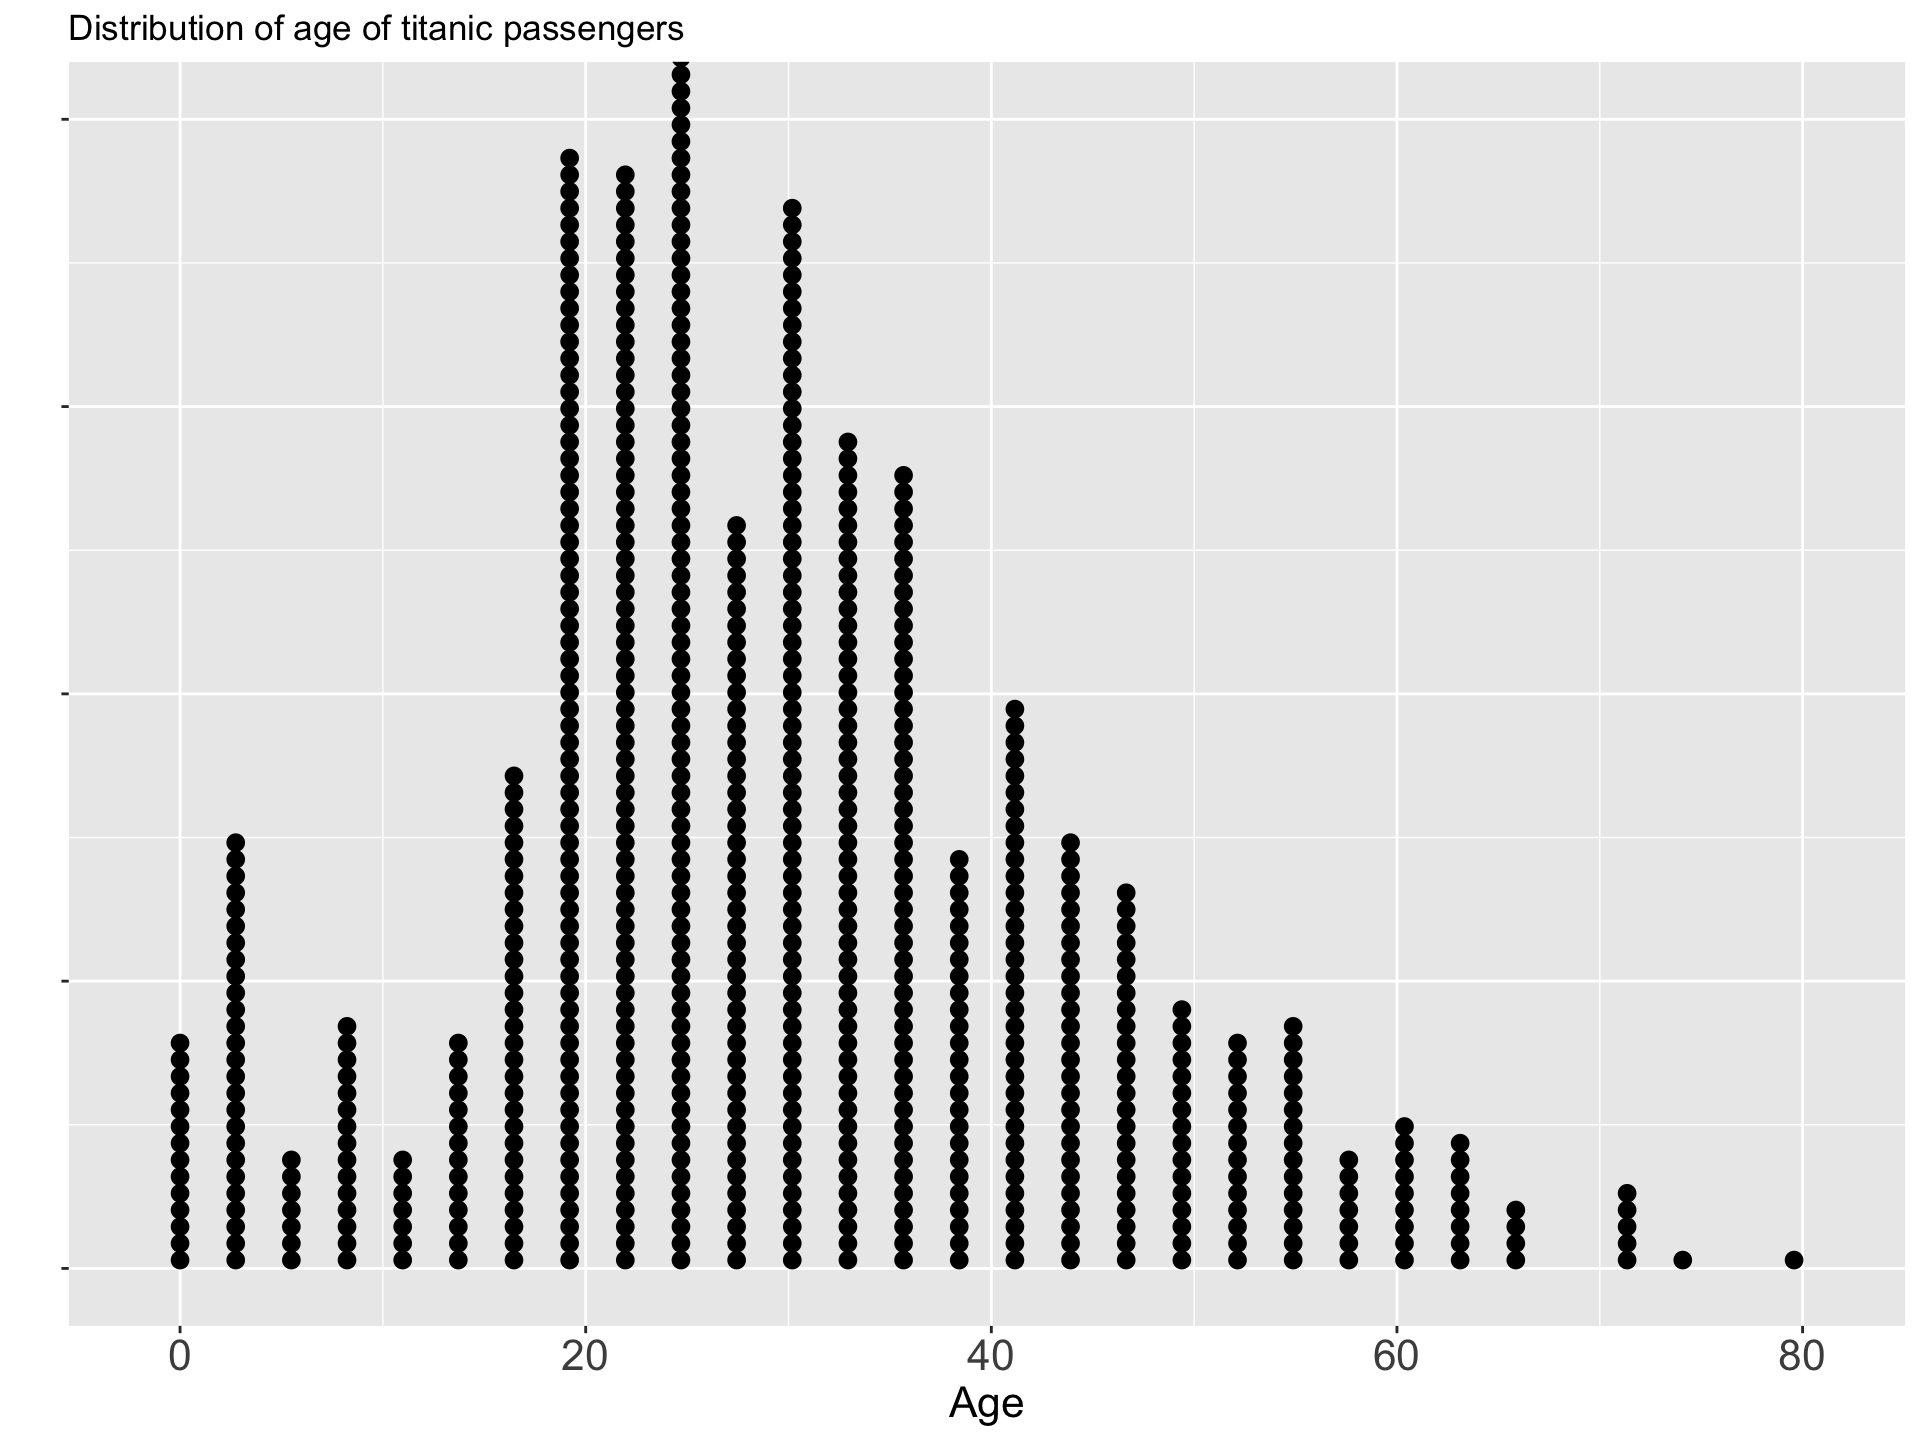
\includegraphics[width=0.8\linewidth]{figure/dotplot-1} \end{center}

\textbf{VI Box plot (Box and whisker plot)}

\begin{itemize}
\tightlist
\item
  Box plot is also a useful method of representing the behavior of a data set or comparing two or more data sets.
\item
  Box plot is constructed by identifying five statistics from the data set as largest value, smallest values, median, Q1 and Q3.
\end{itemize}

\begin{center}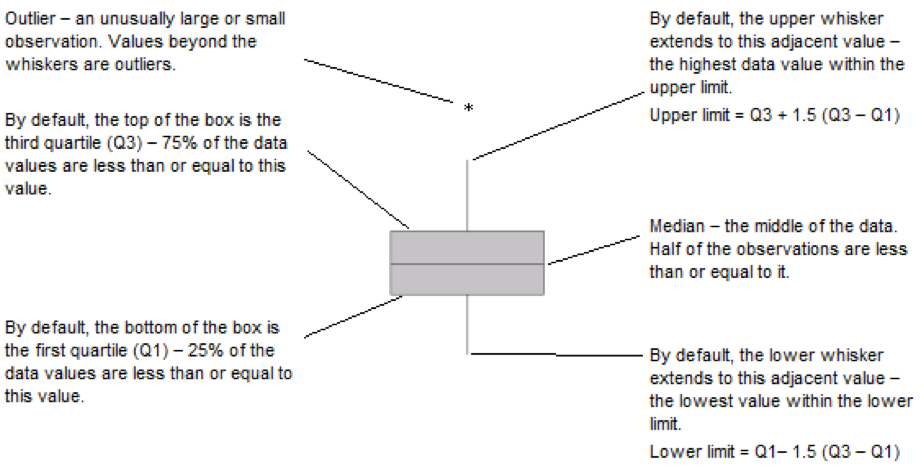
\includegraphics[width=1\linewidth]{figure/boxplot} \end{center}

Example:

Construct a box plot for the following data set (Marks of students)

\[\text{52, 88, 56, 79, 72, 91,  85, 88, 68, 63, 76, 73, 86, 95, 12, 69}\]

Xmin = 12 Xmax = 95 Q1 =64.25 Q2 = Median = 74.5 Q3 = 87.5

\begin{center}
\includegraphics[width=1\linewidth]{figure/box61-1} \end{center}

\begin{center}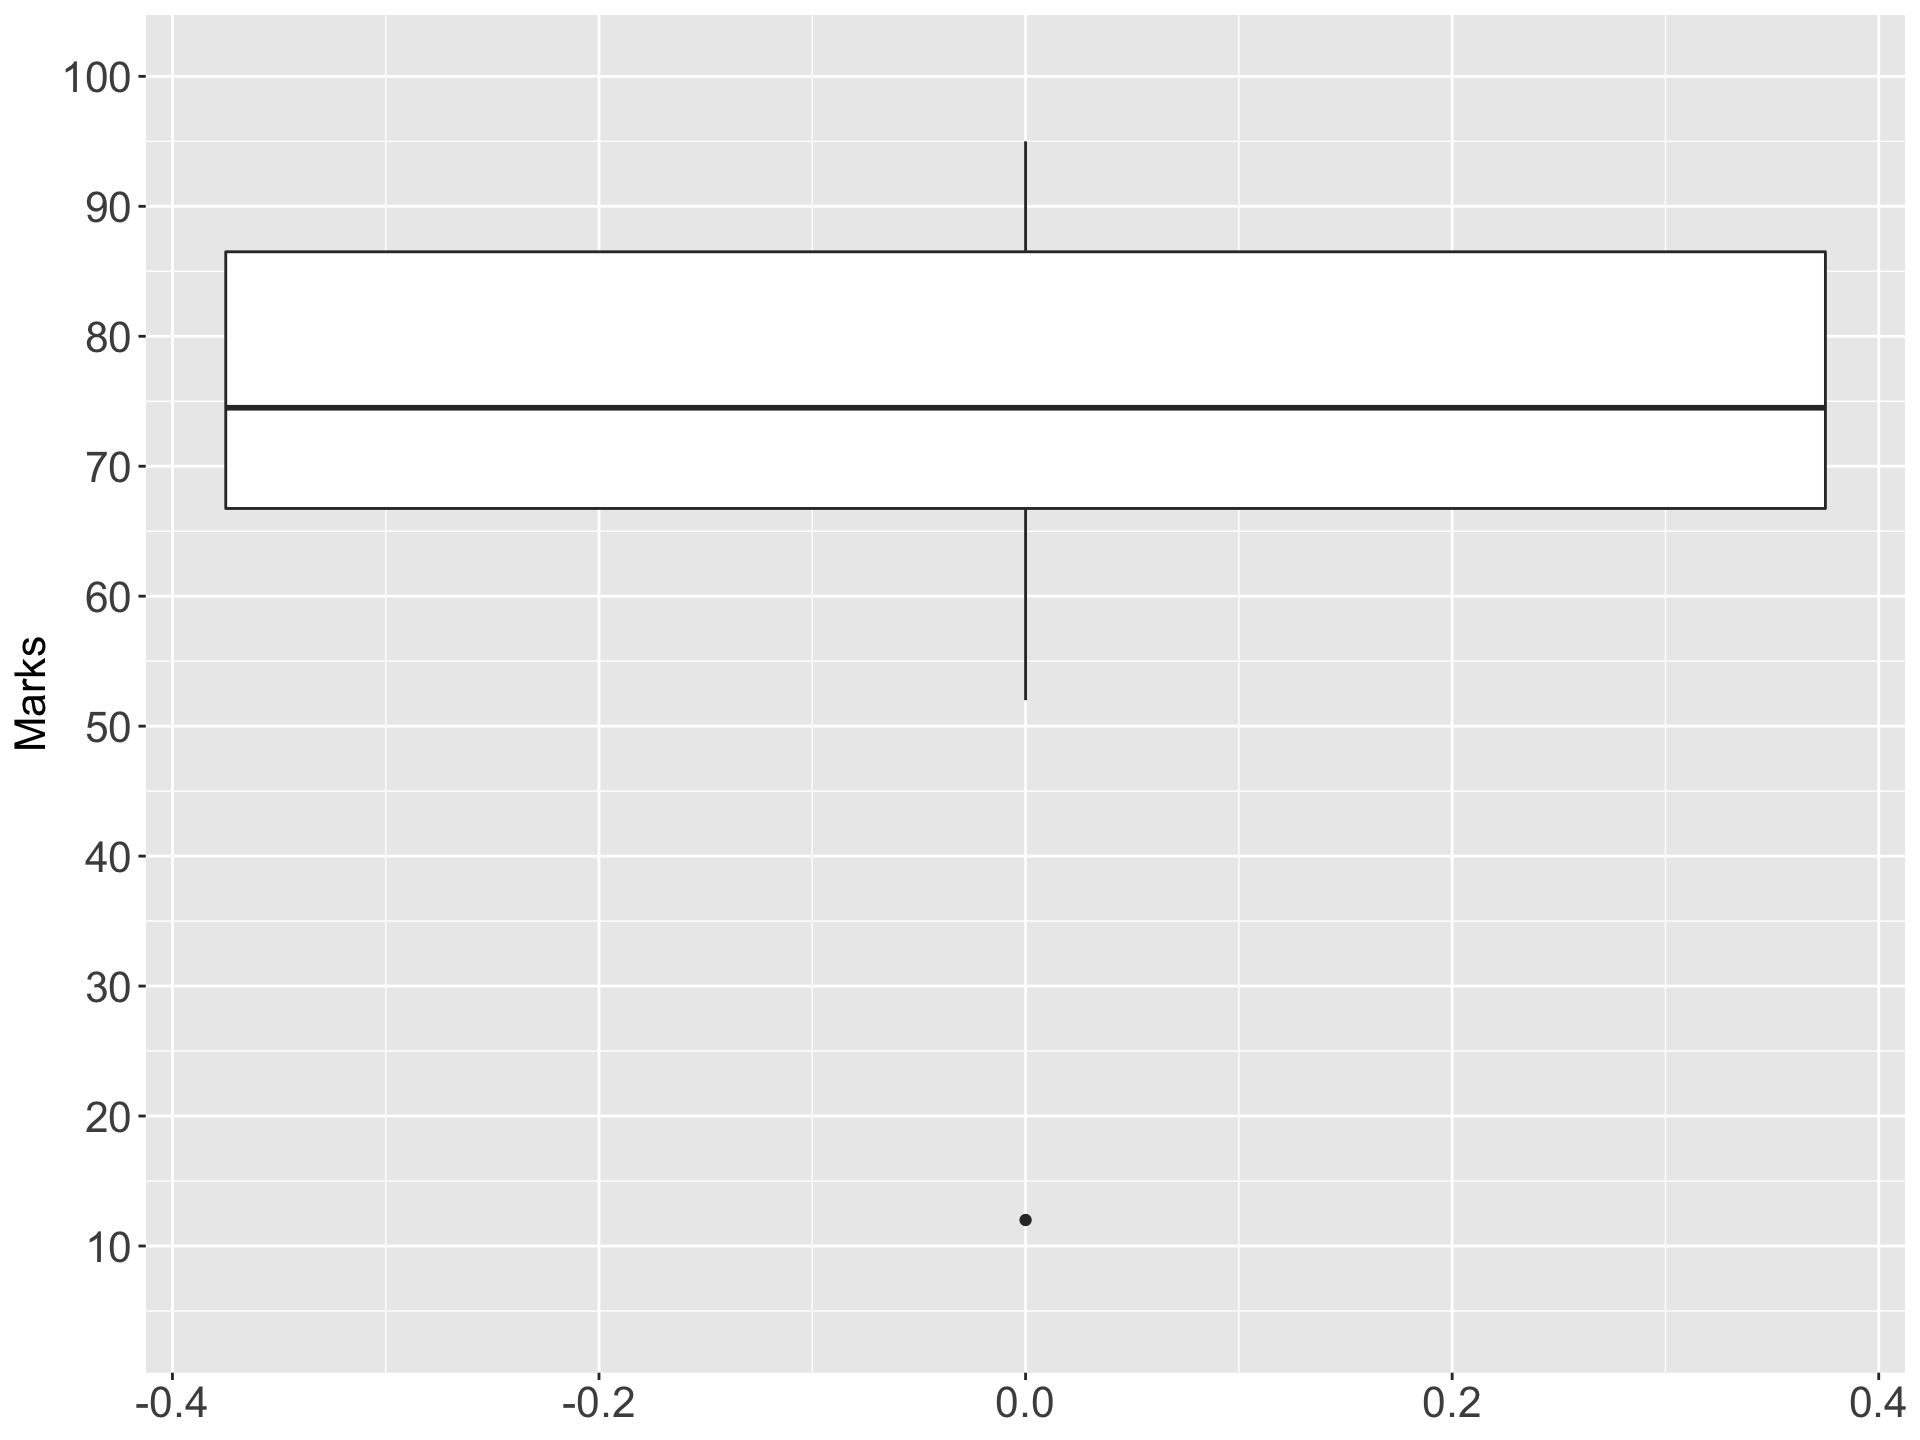
\includegraphics[width=0.8\linewidth]{figure/boxplot-1} \end{center}

\begin{center}\includegraphics[width=0.8\linewidth]{figure/boxplot2-1} \end{center}

\begin{center}\includegraphics[width=0.8\linewidth]{figure/boxplot3-1} \end{center}

\textbf{VII Violin plot}

\begin{itemize}
\tightlist
\item
  A violin plot is a method of plotting quantitative data.
\item
  It is similar to a box plot, with the addition of a rotated kernel density plot on each side.
\item
  Violin plots are similar to box plots, except that they also show the probability density of the data at different values, usually smoothed by a kernel density estimator.
\end{itemize}

\begin{center}\includegraphics[width=0.8\linewidth]{figure/violin1-1} \end{center}

\begin{center}\includegraphics[width=0.8\linewidth]{figure/violin2-1} \end{center}

\newpage

\hypertarget{summary-measures}{%
\section{Summary Measures}\label{summary-measures}}

\begin{itemize}
\item
  Although frequency distribution serves useful purpose, there are many situations that require other types of data summarization.
\item
  What we need in many instances is the ability to summarize the data by means of a single number called a descriptive measure.
\item
  Descriptive measures may be computed from the data of a sample or the data of a population. To distinguish between them we have the following definitions.
\end{itemize}

\textbf{Definitions}

\begin{itemize}
\item
  A descriptive measure computed from the data of a sample is called a \textbf{statistic}.
\item
  A descriptive measure computed from the data of a population is called a \textbf{parameter}.
\end{itemize}

\hypertarget{measures-of-central-tendency}{%
\subsection{Measures of Central Tendency}\label{measures-of-central-tendency}}

\begin{itemize}
\item
  \textbf{Measure of central tendency} yield information about the center, or middle part, of a group of numbers.
\item
  Eg: Mode, Median, Arithmetic Mean, Geometric mean, Harmonic Mean, Quadratic Mean, Quartiles, Deciles, and Percentiles
\end{itemize}

\hypertarget{mode}{%
\subsubsection{Mode}\label{mode}}

\begin{itemize}
\item
  The Mode is the most frequently occuring value in a set of data
\item
  Organizing the data into an ordered array (an ordering of the numbers from smallest to largest) helps to locate the mode.
\item
  A series having only one mode is called as \textbf{uni-modal}
\item
  In the case of a tie for the most frequent occuring value, two modes are listed. Then the data are set to be \textbf{bimodal}
\item
  If a set of data is not exactly bimodal but contains two values that are more dominant than others, some researchers take the liberty of referring to the data set as bimodal even without an \emph{exact tie} for the mode.
\item
  Data sets with more than two modes are referred to as \textbf{multimodal}.
\item
  The mode is an appropriate measure of central tendency for nominal-level data.
\item
  The mode can be used to determine which category occurs most frequently.
\end{itemize}

\textbf{For ungrouped data}

\textbf{Example 01:} Find mode of the following datasets

Dataset 1: 12, 14, 10, 8, 6, 8, 15, 8

\begin{center}\includegraphics[width=1\linewidth]{figure/mode1-1} \end{center}

Dataset 2: 40, 44, 57, 48, 78

\begin{center}\includegraphics[width=1\linewidth]{figure/mode2-1} \end{center}

Dataset 3: 42, 45, 55, 50, 45, 40, 55, 45, 52, 55, 54

\begin{center}\includegraphics[width=1\linewidth]{figure/mode3-1} \end{center}

\textbf{For grouped frequency data}

\textbf{Example 02:} Find mode of the following data

\begin{longtable}[]{@{}ll@{}}
\toprule
Marks & Number of students\tabularnewline
\midrule
\endhead
20 & 8\tabularnewline
30 & 10\tabularnewline
40 & 16\tabularnewline
50 & 8\tabularnewline
60 & 5\tabularnewline
70 & 3\tabularnewline
\bottomrule
\end{longtable}

\begin{itemize}
\tightlist
\item
  Advantages and disadvantages of mode
\end{itemize}

\textbf{Advantages}

\begin{itemize}
\tightlist
\item
  Easy to understand
\item
  Easy to calculate
\item
  Not affected by extreme values in the dataset
\item
  Good for qualitative data
\end{itemize}

\textbf{Disadvantages}

\begin{itemize}
\tightlist
\item
  Not suitable for further mathematical calculations
\item
  There may be more than one mode for a given dataset
\item
  It is not based upon all the observations
\item
  In some cases, we may not be able to find a mode for a given dataset
\end{itemize}

\hypertarget{median}{%
\subsubsection{Median}\label{median}}

\begin{itemize}
\item
  The median is the middle value in an ordered array of numbers.
\item
  Median divides the series into equal parts
\item
  The following steps are used to determine the median.
\item
  STEP 1: Arrange the observations in an ordered data array.
\item
  STEP 2: For an \textbf{odd number} of terms, find the middle term of the ordered array. It is the median.
\item
  STEP 3: For an \textbf{even number} of terms, find the arithmetic mean of the middle two terms. This arithmetic mean is the median.
\end{itemize}

\[Median = \text{the }(\frac{n+1}{2})\text{th item in the data array} \]

\begin{itemize}
\tightlist
\item
  The level of data measurement must be at least ordinal for a median to be meaningful.
\end{itemize}

\textbf{Example 1:} Find the median of the dataset 1, 8, 6, 3, 2

\begin{center}\includegraphics[width=1\linewidth]{figure/median1-1} \end{center}

\textbf{Example 2:} Find the median of the dataset 8, 9, 1, 2, 14, 12

\begin{center}\includegraphics[width=1\linewidth]{figure/median2-1} \end{center}

\begin{itemize}
\tightlist
\item
  Advantages and disadvantages of median
\end{itemize}

\textbf{Advantages}

\begin{itemize}
\tightlist
\item
  Simple to understand
\item
  Easy to calculate
\item
  Not affected by extreme values in the dataset
\item
  Can be calculated even for qualitative variables (ordinal scale data)
\end{itemize}

\textbf{Disadvantages}

\begin{itemize}
\tightlist
\item
  It is not based upon all the observations
\end{itemize}

\hypertarget{arithmetic-mean}{%
\subsubsection{Arithmetic Mean}\label{arithmetic-mean}}

\begin{itemize}
\item
  The arithmetic mean (usually called mean) is the sum of all observations divided by the total number of observations.
\item
  Population Mean

  \begin{itemize}
  \item
    The poupulation mean us represented by the Greek letter \(mu\) (\(\mu\)).
  \item
    Let, \(N\) is the number of terms in the population.
  \end{itemize}
\end{itemize}

\[\mu = \frac{\sum{x}}{N}=\frac{x_1+x_2+x_3+...+x_N}{N}\]

\begin{itemize}
\item
  Sample Mean

  \begin{itemize}
  \tightlist
  \item
    The sample mean is represented by \(\bar{x}\)
  \item
    Let, \(n\) is the number of terms in the sample
    \[\bar{x} = \frac{\sum{x}}{n}=\frac{x_1+x_2+x_3+...+x_n}{n}\]
  \end{itemize}
\item
  It is inappropriate to use the mean to analyse data that are not at least interval level in measurement.
\end{itemize}

\textbf{Example 1:} Calculate the mean from the following data

\begin{longtable}[]{@{}lllllllllll@{}}
\toprule
Student & 1 & 2 & 3 & 4 & 5 & 6 & 7 & 8 & 9 & 10\tabularnewline
\midrule
\endhead
Marks & 40 & 50 & 53 & 78 & 58 & 60 & 73 & 35 & 43 & 48\tabularnewline
\bottomrule
\end{longtable}

\begin{center}\includegraphics[width=1\linewidth]{figure/mean1-1} \end{center}

\begin{itemize}
\tightlist
\item
  Advantages and disadvantages of arithmetic mean
\end{itemize}

\textbf{Advantages}

\begin{itemize}
\tightlist
\item
  Simple to understand
\item
  Easy to calculate
\item
  Based on all the observations
\item
  Well defined
\item
  Unique
\item
  Can be used in further calculation
\end{itemize}

\textbf{Disadvantages}

\begin{itemize}
\tightlist
\item
  Can be affected by extreme values in the dataset
\item
  May lead to false conclusions
\item
  Only applicable to quantitative data (not applicable to qualitative data)
\end{itemize}

\textbf{Empirical relationship between mean, mode, median}

\begin{itemize}
\tightlist
\item
  In case of symmetrical distribution, mean, median and mode coincide \((mean = meadian= mode)\)
\end{itemize}

\begin{center}\includegraphics[width=1\linewidth]{figure/box24 -1} \end{center}

\begin{itemize}
\tightlist
\item
  For a moderately asymmetrical distribution, the following relationship exists \(Mean – Mode = 3(Mean - Median)\)
\end{itemize}

\begin{center}\includegraphics[width=1\linewidth]{figure/box25 -1} \end{center}

\textbf{Choice between mean and median}

\begin{itemize}
\tightlist
\item
  Mean is very sensitive to outliers.Median is not sensitive to outliers
\item
  When there are outliers in a data set, median is more appropriate than mean
\end{itemize}

\hypertarget{quartiles-deciles-and-percentiles}{%
\subsubsection{Quartiles, Deciles and Percentiles}\label{quartiles-deciles-and-percentiles}}

\begin{itemize}
\tightlist
\item
  Median divides the data set into two equal parts.
\item
  There are other values which divide the data set into a number of equal parts
\item
  Those are Quartiles, Deciles and Percentiles
\end{itemize}

\textbf{\emph{(a) Quartiles (Q) -- Quartiles divide an array into four equal parts}}

\[Q_i = \text{the }\frac{i}{4}(n+1)\text{th item in the data array} \]

\textbf{\emph{(b) Deciles (D) -- Deciles divide an array into ten equal parts}}

\[D_i = \text{the }\frac{i}{10}(n+1)\text{th item in the data array} \]

\textbf{\emph{(c) Percentiles (P) -- Percentiles divide an array into 100 equal parts}}

\[P_i = \text{the }\frac{i}{100}(n+1)\text{th item in the data array} \]

\hypertarget{measures-of-variability}{%
\subsection{Measures of Variability}\label{measures-of-variability}}

\begin{itemize}
\item
  Measure of central tendency yield information about particular points of a data set.
\item
  However, business researchers can use another group of analytic tools to describe a set of data.
\item
  These tools are measures of variability, which describe the spread or the dispersion of a set of data.
\item
  Using measures of variability in conjunction with measures of central tendency makes possible a more complete numerical description of the data.
\item
  This section focuses on seven measures of variability for ungrouped data: range, interquartile range, variance, standard deviation, z score and coefficient of variation.
\end{itemize}

\hypertarget{range}{%
\subsubsection{Range}\label{range}}

\begin{itemize}
\tightlist
\item
  The range is the difference between the largest value of a data set and the smallest value.
\end{itemize}

\[Range = Maximum - Minimum\]

\begin{itemize}
\item
  One important use of the range is in quality assurance, where the range is used to construct control charts
\item
  Advantages and disadvantages of range
\end{itemize}

\textbf{Advantages}

\begin{itemize}
\tightlist
\item
  Easy to understand and calculate
\end{itemize}

\textbf{Disadvantages}

\begin{itemize}
\tightlist
\item
  Consider only the highest and lowest values of the data and fails to take account of any other observations in the dataset
\item
  Heavily influenced by extreme values
\end{itemize}

\hypertarget{interquartile-range-iqr}{%
\subsubsection{Interquartile Range (IQR)}\label{interquartile-range-iqr}}

\begin{itemize}
\item
  We use the interquartile range (IQR) to measure the spread of a data around the median (M).
\item
  The interquartile range is the range of values between the first and third quartile.
\item
  Essentially it is the range of the middle 50\% of the data and is determined by computing the value of \(Q_3 - Q_1\).
\item
  The interquartile range is especially useful in situations where data users are more interested in values towards the middle and less interested in extremes.
\item
  The interquartile range is used in the construction of box and whisker plots.
\item
  By eliminating the lowest 25\% and the highest 25\% of the items in a series, we are left with the central 50\% , which are ordinarily free of extreme values.
\end{itemize}

\textbf{Advantages}

\begin{itemize}
\tightlist
\item
  Easy to understand and calculate
\item
  Not influenced by extreme values
\end{itemize}

\textbf{Disadvantages}

\begin{itemize}
\tightlist
\item
  Ignore the first \(25\%\) and the last \(25\%\) in the dataset
\end{itemize}

\hypertarget{variance-and-standard-deviation}{%
\subsubsection{Variance and Standard Deviation}\label{variance-and-standard-deviation}}

\begin{itemize}
\tightlist
\item
  To measure the spread of data around the mean, we use the standard deviation (S).
\item
  The variance and standard deviation are two very popular measures of dispersion.
\item
  These measures are not meaningful unless the data are at least interval-level data.
\item
  Their formulations are categorized into whether to evaluate from a population or from a sample.
\end{itemize}

\emph{NOTE}

\begin{itemize}
\item
  Sum of deviations from the arithmetic mean is always zero.
  \[{\sum{(x-\mu)} = 0}\]
\item
  This property requires considering the alternative ways to obtain measure of variability.
\end{itemize}

\hypertarget{variance}{%
\paragraph{Variance}\label{variance}}

\begin{itemize}
\item
  The \textbf{variance} is the average of the squared deviations about the mean for a set of numbers.
\item
  The population variance is denoted by \(\sigma^2\)
\end{itemize}

\[\sigma^2 = \frac{\sum(x-\mu)^2}{N}\]

\begin{itemize}
\item
  \emph{The sum of the squared deviations about the mean of a set of values} - called the \textbf{sum of squares of} \(x\) and sometimes abbreviated as \(SS_x\)
\item
  Because the variance is computed from squared deviations, the final result is expressed in terms of squared units of measurements.
\item
  Statistics measured in squared units are problematic to interpret.
\end{itemize}

\hypertarget{standard-deviation}{%
\paragraph{Standard Deviation}\label{standard-deviation}}

\begin{itemize}
\item
  The standard deviation is the square root of the variance.
\item
  The population standard deviation is denoted by \(\sigma\)
\end{itemize}

\[\sigma = \sqrt{\frac{\sum(x-\mu)^2}{N}}=\sqrt{\sigma^2}\]

\begin{itemize}
\tightlist
\item
  One feature of standard deviation that distinguishes it from a variance is that the standard deviation is expressed in the same units as the raw data, whereas the variance is expressed in those units squared.
\end{itemize}

\textbf{Advantages}

\begin{itemize}
\tightlist
\item
  Based on all the observations
\item
  Since this is based on arithmetic mean, it has all the merits of it
\item
  The most important and widely used measure of dispersion
\end{itemize}

\textbf{Disadvantages}

\begin{itemize}
\tightlist
\item
  Not easy to understand and difficult to calculate
\item
  Gives more weight to extreme values, because the values are squared up
\end{itemize}

\hypertarget{empirical-rule}{%
\subsubsection{Empirical Rule}\label{empirical-rule}}

\begin{itemize}
\item
  The empirical rule is an important rule of thumb that is used to state the approximate percentage of values that lie within a given number of standard deviations from the mean of a set of data \textbf{if the data are normally distributed}
\item
  The empirical rule is used only for three numbers of standard deviations: \(1\sigma\), \(2\sigma\), \(3\sigma\)
\end{itemize}

\begin{longtable}[]{@{}ll@{}}
\toprule
Distance from the mean & Values within distance\tabularnewline
\midrule
\endhead
\(\mu\pm1\sigma\) & \(68\%\)\tabularnewline
\(\mu\pm2\sigma\) & \(95\%\)\tabularnewline
\(\mu\pm3\sigma\) & \(99.7\%\)\tabularnewline
\bottomrule
\end{longtable}

\begin{center}\includegraphics[width=1\linewidth]{figure/emp -1} \end{center}

\begin{itemize}
\tightlist
\item
  If a set of data is normally distributed, or bell shaped, approximately \(68\%\) of the data values are within one standard deviation of the mean, \(95\%\) are within two standard deviations, and almost \(100\%\) are within three standard deviations.
\end{itemize}

\hypertarget{population-versus-sample-variance-and-standard-deviations}{%
\subsubsection{Population versus sample variance and standard deviations}\label{population-versus-sample-variance-and-standard-deviations}}

\begin{itemize}
\item
  The sample variance is denoted by \(s^2\) and the sample standard deviation by \(s\).
\item
  The main use for sample variances and standard deviations is as estimators of population variances and standard deviations.
\item
  Thus, computation of the sample variance and standard deviation differs slightly from computation of the population variance and standard deviation.
\item
  Both the sample variance and sample standard deviation use \(n-1\)int he denominator instead of \(n\) because using \(n\) in the denominator of a sample variance results in a statistic that tends to underestimate the population variance.
\item
  While discussion of the properties of \emph{good estimator} is beyond the scope of this course, one of the properties of a good estimator is being \emph{unbiased}.
\item
  Whereas, using \(n\) in the denominator of the sample variance makes it a \emph{biased} estimator, using \(n-1\) allows it to be an \emph{unbiased} estimator, which is a desirable property in inferential statistics.
\end{itemize}

\textbf{Sample variance}

\[s^2 = \frac{\sum{(x-\bar{x})^2}}{n-1}\]

\textbf{Sample standard deviation}

\[s = \sqrt{\frac{\sum{(x-\bar{x})^2}}{n-1}}= \sqrt{s^2}\]

\hypertarget{computational-formulas-for-variance-and-standard-deviation}{%
\subsubsection{Computational formulas for variance and standard deviation}\label{computational-formulas-for-variance-and-standard-deviation}}

\begin{itemize}
\item
  An alternative method of computing variance and standard deviation, sometimes referred to as the computational method or shortcut method, is available.
\item
  Algebraically,
\end{itemize}

\[\sum{(x-\mu)^2}= \sum{x^2}- \frac{(\sum x)^2}{N}\]

\begin{center}\includegraphics[width=1\linewidth]{figure/variance1-1} \end{center}

and

\[\sum{(x-\bar{x})^2}= \sum{x^2}- \frac{(\sum x)^2}{n}\]

\begin{center}\includegraphics[width=1\linewidth]{figure/variance2-1} \end{center}

\begin{itemize}
\tightlist
\item
  Substituting these equivalent expressions into the original formulas for variance and standard deviation yields the following computational formulas.
\end{itemize}

\textbf{Computational formula for population variance and standard deviation}

\[\sigma^2 = \frac{\sum{x^2}- \frac{(\sum x)^2}{N}}{N}\]

\[\sigma = \sqrt{\sigma^2}\]

\textbf{Computational formula for sample variance and standard deviation}

\[s^2 = \frac{\sum{x^2}- \frac{(\sum x)^2}{n}}{n-1}\]

\[s = \sqrt{s^2}\]

\begin{itemize}
\tightlist
\item
  For situations in which the mean is already computed or is given, alternative forms of these formulas are:
\end{itemize}

\[\sigma^2 = \frac{\sum{x^2}-N\mu^2}{N}\]

\[s^2 = \frac{\sum{x^2}-n(\bar{x})^2}{n-1}\]

\hypertarget{coefficient-of-variation}{%
\subsubsection{Coefficient of variation}\label{coefficient-of-variation}}

\begin{itemize}
\item
  In general, for two variables measured with he same units (eg: two groups of people both weighed in kg), the group with the larger variance and standard deviation has n=more variability among their scores.
\item
  The unit of measure affects the size od the variance.
\item
  The same population weights, expressed in `grams' rather than kg would have a larger variance and standard deviation.
\item
  The \emph{coefficient of variation}, a measure of relative variability gets around this difficulty and makes it possible to compare variability across variables measured in different units.
\item
  The coefficient of variation is the ratio of the standard deviation to the mean, expressed as a percentage and is denoted CV.
\end{itemize}

\[CV = \frac{\sigma}{\mu}(100)\]

\textbf{Using median and quartile deviation}

\[CV = \frac{\frac{Q_3 - Q_1}{2}}{Median}(100)\]

\begin{itemize}
\item
  The coefficient of variation essentially is a relative comparison of a standard deviation to its mean.
\item
  The coefficient of variation can be useful in comparing standard deviations that have been computed from data with different means.
\item
  The choice of whether to use a coefficient of variation or raw standard deviations to compare multiple standard deviations is a matter of preference
\item
  The coefficient of variation also provides and optional method of interpreting the value of a standard deviation.
\end{itemize}

\hypertarget{measures-of-shape}{%
\subsection{Measures of Shape}\label{measures-of-shape}}

\begin{itemize}
\item
  Measures of shape are tools that can be used to describe the shape of a distribution of data.
\item
  In this section, we examine two measures of shapes: skewness and Kurtosis.
\end{itemize}

\hypertarget{skewness}{%
\subsubsection{Skewness}\label{skewness}}

\begin{itemize}
\item
  A distribution of data in which the right half is a mirror image of the left half is said to be \emph{symmetrical.}
\item
  One example of a symmetrical distribution is the normal distribution, or bell curve.
\item
  \textbf{Skewness} is a measure of symmetry, or more precisely, the lack of symmetry
\item
  The measures of asymmetry are called as measures of skewness.
\item
  The skewed portion is the long, thin part of the curve
\end{itemize}

\textbf{Skewness and the relationship of the mean, median and mode}

\begin{itemize}
\item
  The concept of skewness helps us to understand the relationship between the mean, median and mode.
\item
  In a unimodal distribution (distribution with a single peak or mode) that is skewed, the mode is the apex (high point) of the curve and the median is the middle value.
\item
  The mean tends to be located toward the tail of the distribution, because the mean is affected by all values, including the extreme ones.
\item
  A bell-shaped or normal distribution with the mean, median and mode all at the centre of the distribution has no skewness.
\end{itemize}

\begin{figure}

{\centering \includegraphics[width=1\linewidth]{figure/skewness} 

}

\caption{Relationship of mean, median and mode for different types of skewness}\label{fig:unnamed-chunk-23}
\end{figure}

\hypertarget{pearsonian-coefficient-of-skewness}{%
\paragraph{Pearsonian coefficient of skewness}\label{pearsonian-coefficient-of-skewness}}

\begin{itemize}
\tightlist
\item
  This coefficient compares the mean and median in light of the magnitude of the standard deviation
\end{itemize}

\[S_k = \frac{3(\mu-M_d)}{\sigma}\]

where \(S_k\) = coefficient of skewness, \(M_d\) = median

\begin{itemize}
\item
  Note that if the distribution is symmetrical, the mean and median are the same value and hence the coefficient of skewness is equal to zero.
\item
  If the value of \(S_k\) is positive, the distribution is positively skewed.
\item
  If the value of \(S_k\) is negative, the distribution is negatively skewed.
\item
  The greater the magnitude of \(S_k\), the more skewed is the distribution.
\end{itemize}

\hypertarget{kurtosis}{%
\subsubsection{Kurtosis}\label{kurtosis}}

\begin{itemize}
\item
  Kurtosis describes the amount of peakedness of a distribution.
\item
  \textbf{Kurtosis} is a measure of whether the data are peaked or flat relative to a normal distribution
\item
  Distributions that are high and thin are referred to as \textbf{leptokurtic} distributions.
\item
  Distributions that are flat and spread out are referred to as \textbf{platykurtic} distributions.
\item
  Between the above two types are distributions that are more `normal' in shape, referred to as \textbf{mesokurtic} distributions
\end{itemize}

\begin{figure}

{\centering \includegraphics[width=1\linewidth]{figure/kurtosis} 

}

\caption{Types of kurtosis}\label{fig:unnamed-chunk-24}
\end{figure}

\hypertarget{measures-of-association}{%
\subsection{Measures of Association}\label{measures-of-association}}

\begin{itemize}
\tightlist
\item
  Many times in business it is important to explore the relationship between two numerical variables
\item
  Measures of association are statistics that yeild information about the relatedness of numerical variables.
\item
  In this section, we discuss only one measure of association, correlation, and d so only for two numerical variables.
\end{itemize}

\hypertarget{scatter-plot}{%
\subsubsection{Scatter plot}\label{scatter-plot}}

\begin{itemize}
\tightlist
\item
  A scatter plot is a two dimensional graph of pairs of points from \textbf{two numerical} variables
\item
  In a quantitative bi-variate dataset, we have a \((x,y)\) pair for each sampling unit, where \(x\) denotes the independent variable and \(y\) denotes the dependent variable.
\item
  Each \((x,y)\) pair can be considered as a point on the Cartesian plan.
\item
  Scatter plot is a plot of all the \((x,y)\) pairs in the dataset.
\item
  The purpose of scatter plot is to illustrate any relationship between two quantitative variables.

  \begin{itemize}
  \tightlist
  \item
    If the variables are related, what kind of relationship it is, linear or nonlinear?
  \item
    If the relationship is linear, the scatter plot will show whether it is negative or positive.
  \end{itemize}
\end{itemize}

\textbf{Example:} \emph{Edgar Anderson's Iris Data}

This famous (Fisher's or Anderson's) iris data set gives the measurements in centimeters of the variables sepal length and width and petal length and width, respectively, for 50 flowers from each of 3 species of iris. The species are Iris setosa, versicolor, and virginica.

\begin{center}\includegraphics[width=0.8\linewidth]{figure/scatterplot-1} \end{center}

\hypertarget{correlation}{%
\subsubsection{Correlation}\label{correlation}}

\begin{itemize}
\tightlist
\item
  Correlation is a measure of the degree of relatedness of two or more variables.
\item
  Several measures of correlation are available , the selection of which depends mostly on the level of data being analysed.
\item
  Ideally, researchers would like to calculate \(\rho\), the \textbf{population} coefficient of correlation.
\item
  However, because researchers virtually always deal with sample data, this section introduces a widely used sample coefficient of correlation, \(r\).
\item
  This measure is applicable \textbf{only if both variables being analysed have at least an interval level of data}
\end{itemize}

\textbf{Pearson product-moment correlation coefficient} (\(r\))

\begin{itemize}
\tightlist
\item
  The statistic \(r\) is the Pearson product-moment correlation coefficient, named after Karl Pearson (1857 - 1936).
\item
  The tern \(r\) is a measure of the \textbf{linear} correlation of two variables.
\item
  It is a number that ranges from -1 to 0 to +1, representing th strength of the linear relationship between the variables.
\item
  An \(r\) value of \(+1\) denotes a perfect \textbf{linear} positive relationship between two variables.
\item
  An \(r\) value of \(-1\) denotes a perfect \textbf{linear} negative relationship between two variables, which indicates an inverse relationship between two variables: as one variable gets larger, the other gets smaller.
\item
  An \(r\) value of 0 means no \textbf{linear} relationship is present between the two variables.
\end{itemize}

\[ r = \frac{\sum(x-\bar{x})(y-\bar{y})}{\sqrt{\sum(x-\bar{x})^2\sum(y-\bar{y})^2}}\]

\[ r = \frac{\sum{xy} - \frac{(\sum x\sum y)}{n}}{\sqrt{[\sum{x^2- \frac{(\sum{x})^2}{n}}][\sum y^2-\frac{(\sum y)^2}{n}]}}\]

\begin{itemize}
\tightlist
\item
  Examples: Following figure shows five different degrees of correlation:
\end{itemize}

\begin{center}\includegraphics[width=1\linewidth]{figure/cor-1} \end{center}

\textbf{NOTE}

\begin{itemize}
\tightlist
\item
  When \(r=0\), it signifies there is \textbf{no linear} relationship between the two variables. (There can be a non-linear relationship, Figure (e))
\item
  Figure (e): There is a very strong curvilinear relationship. But there is \textbf{no linear} relationship.
\end{itemize}

\hypertarget{references}{%
\subsection*{References}\label{references}}
\addcontentsline{toc}{subsection}{References}

Black, K., Asafu-Adjaye, J., Khan, N., Perera, N., Edwards, P., \& Harris, M. (2007). \emph{Australasian business statistics}. John Wiley \& Sons.

\newpage

\pagenumbering{arabic}

\hypertarget{tutorial}{%
\section{Tutorial}\label{tutorial}}

\hypertarget{chapter-6-descriptive-statistics}{%
\subsection*{Chapter 6: Descriptive Statistics}\label{chapter-6-descriptive-statistics}}
\addcontentsline{toc}{subsection}{Chapter 6: Descriptive Statistics}

\begin{enumerate}
\def\labelenumi{\arabic{enumi}.}
\tightlist
\item
  A power company in Sri Lanka designs and manufactures power distribution switchboards for hospitals, bridges, airports, highways and water treatment plants. Power company marketing director wants to determine client satisfaction with their products and services. He developed a questionnaire that yields a satisfaction score between 0 and 100 for participant responses. A random sample of 50 of the company's 1000 clients is asked to complete a satisfaction survey. The satisfaction scores for the 50 participants are averaged to produce a mean satisfaction score.
\end{enumerate}

\begin{enumerate}
\def\labelenumi{\alph{enumi}.}
\tightlist
\item
  What is the objective of this study?
\item
  What is the population for this study?
\item
  What is the sample for this study?
\item
  What is the statistic for this study?
\item
  What would be a parameter for this study?
\end{enumerate}

\begin{enumerate}
\def\labelenumi{\arabic{enumi}.}
\setcounter{enumi}{1}
\tightlist
\item
  Determine the type and the scale of measurement of the following variables
\end{enumerate}

\begin{enumerate}
\def\labelenumi{\alph{enumi}.}
\tightlist
\item
  The time required to produce an item on an assembly line
\item
  the number of litres of milk a family drinks in a week
\item
  The ranking of 50 students in your class after their overall performance have been designated as excellent, good, satisfactory or poor
\item
  The telephone area code of clients in Australia
\item
  The age of each of your batch mates
\item
  The sales at the local pizza restaurant each month
\item
  A student index number
\item
  The response time of emergency services
\item
  The number of tickets sold at a ticket counter on any given day
\item
  Monthly maximum air temperature
\end{enumerate}

\begin{enumerate}
\def\labelenumi{\arabic{enumi}.}
\setcounter{enumi}{2}
\item
  The grades of 30 students for Statistics are as follows:

  B, C, B, D, B, C, C, A , B, C,

  C, B, E, B, B, D, D, F, B, D,

  D, A, B, A, B, C, E, A, A, E
\end{enumerate}

\begin{enumerate}
\def\labelenumi{\alph{enumi}.}
\tightlist
\item
  Construct a frequency table with suitable values (eg: absolute frequency, relative frequency, cumulative frequency, cumulative relative frequency)
\end{enumerate}

\begin{enumerate}
\def\labelenumi{\arabic{enumi}.}
\setcounter{enumi}{3}
\item
  The gender type of a group of 10 students are as follows:

  Male, Female, Female, Male, Female
  Female, Male, Male, Female, Female
\end{enumerate}

\begin{enumerate}
\def\labelenumi{\alph{enumi}.}
\tightlist
\item
  Construct a frequency table with suitable values (eg: absolute frequency, relative frequency, cumulative frequency, cumulative relative frequency )
\end{enumerate}

\begin{enumerate}
\def\labelenumi{\arabic{enumi}.}
\setcounter{enumi}{4}
\tightlist
\item
  In a study conducted to investigate the relationship between delivery time and computer-assisted ordering, the following data were gathered from a sample of 40 firms, that 16 use computer-assisted ordering, while 24 do not. Furthermore, past data are used to categorize each firm's delivery times below the industry average, equal to the industry average, or above the industry average. The results obtained are given in the table below.
\end{enumerate}

\begin{longtable}[]{@{}lllll@{}}
\toprule
\begin{minipage}[b]{0.16\columnwidth}\raggedright
Computer Assisted Ordering\strut
\end{minipage} & \begin{minipage}[b]{0.18\columnwidth}\raggedright
Delivery Time Below Industry Average\strut
\end{minipage} & \begin{minipage}[b]{0.19\columnwidth}\raggedright
Delivery Time Equal to Industry Average\strut
\end{minipage} & \begin{minipage}[b]{0.15\columnwidth}\raggedright
Delivery Time Above industry Average\strut
\end{minipage} & \begin{minipage}[b]{0.18\columnwidth}\raggedright
Row Total\strut
\end{minipage}\tabularnewline
\midrule
\endhead
\begin{minipage}[t]{0.16\columnwidth}\raggedright
No\strut
\end{minipage} & \begin{minipage}[t]{0.18\columnwidth}\raggedright
4\strut
\end{minipage} & \begin{minipage}[t]{0.19\columnwidth}\raggedright
12\strut
\end{minipage} & \begin{minipage}[t]{0.15\columnwidth}\raggedright
8\strut
\end{minipage} & \begin{minipage}[t]{0.18\columnwidth}\raggedright
24\strut
\end{minipage}\tabularnewline
\begin{minipage}[t]{0.16\columnwidth}\raggedright
Yes\strut
\end{minipage} & \begin{minipage}[t]{0.18\columnwidth}\raggedright
10\strut
\end{minipage} & \begin{minipage}[t]{0.19\columnwidth}\raggedright
4\strut
\end{minipage} & \begin{minipage}[t]{0.15\columnwidth}\raggedright
2\strut
\end{minipage} & \begin{minipage}[t]{0.18\columnwidth}\raggedright
16\strut
\end{minipage}\tabularnewline
\begin{minipage}[t]{0.16\columnwidth}\raggedright
Total\strut
\end{minipage} & \begin{minipage}[t]{0.18\columnwidth}\raggedright
14\strut
\end{minipage} & \begin{minipage}[t]{0.19\columnwidth}\raggedright
16\strut
\end{minipage} & \begin{minipage}[t]{0.15\columnwidth}\raggedright
10\strut
\end{minipage} & \begin{minipage}[t]{0.18\columnwidth}\raggedright
40\strut
\end{minipage}\tabularnewline
\bottomrule
\end{longtable}

\begin{enumerate}
\def\labelenumi{\alph{enumi})}
\tightlist
\item
  For each row and column total, calculate the corresponding row or column percentage.
\item
  For each cell, calculate the corresponding cell, row, and column percentages.
\item
  Carry out graphical analysis to investigate the relationship between delivery-time performance and computer-assisted ordering.
\item
  What conclusions can be made about the nature of the relationship?
\end{enumerate}

\begin{enumerate}
\def\labelenumi{\arabic{enumi}.}
\setcounter{enumi}{5}
\item
\end{enumerate}

\begin{enumerate}
\def\labelenumi{\alph{enumi})}
\tightlist
\item
  Giving suitable examples distinguish between multiple bar chart and a component bar chart.
\item
  Write down advantages and disadvantages of each chart and when they should be used
\end{enumerate}

\begin{enumerate}
\def\labelenumi{\arabic{enumi}.}
\setcounter{enumi}{6}
\tightlist
\item
  In a study conducted to investigate the effect of wearing helmets in riding motorcycles to reduce the head injuries, the following data were gathered by investigating 151 motorcycle accidents reported during last 10 month period. Out of the total number of cases (151) investigated, only 102 people were wearing helmets properly at the time of the accidents. Out of them, only 9 got severe head injuries. The rest got either minor head injuries or no head injuries at all. Among 49 who were not wearing helmets at the time of the accident, 15 got server head injuries and the rest got minor head injuries or no head injuries at all.
\end{enumerate}

\begin{enumerate}
\def\labelenumi{\alph{enumi})}
\item
  Use an appropriate table to represent the above data and state what conclusions can be drawn from it
\item
  Carry out a suitable graphical analysis to investigate the effect of wearing helmets in riding motorcycles to reduce the head injuries.
\end{enumerate}

\begin{enumerate}
\def\labelenumi{\arabic{enumi}.}
\setcounter{enumi}{7}
\tightlist
\item
  The table below shows a frequency distribution of the weekly wages of 65 employees at the ABC Company. With reference to this table,
\end{enumerate}

\begin{longtable}[]{@{}ll@{}}
\toprule
Wages (in \$) & Number of Employees\tabularnewline
\midrule
\endhead
250.00 - 259.99 & 8\tabularnewline
260.00 - 269.99 & 10\tabularnewline
270.00 - 279.99 & 16\tabularnewline
280.00 - 289.99 & 14\tabularnewline
290.00 - 299.99 & 10\tabularnewline
300.00 - 309.99 & 5\tabularnewline
310.00 - 319.99 & 2\tabularnewline
Total & 65\tabularnewline
\bottomrule
\end{longtable}

\begin{enumerate}
\def\labelenumi{\alph{enumi})}
\tightlist
\item
  Construct a histogram
\item
  Construct a frequency polygon
\item
  Construct a frequency curve
\item
  State what conclusions can be drawn from the above graphical analysis
\end{enumerate}

\begin{enumerate}
\def\labelenumi{\arabic{enumi}.}
\setcounter{enumi}{8}
\tightlist
\item
  The contribution of the agriculture, industrial, and service sector to the Gross Domestic Product (GDP) for each province in Sri Lanka is given in the table below. It is required to investigate whether the contributions are varying from province to province. What kind of graph you would suggest for representing data to serve the purpose. Justify your answer. Sketch the proposed graph.
\end{enumerate}

\begin{center}\includegraphics[width=1\linewidth]{figure/C6T1} \end{center}

\begin{enumerate}
\def\labelenumi{\arabic{enumi}.}
\setcounter{enumi}{9}
\tightlist
\item
  Marks of 16 students are given below.
\end{enumerate}

\[\text{52, 88, 56, 79, 72, 91,  85, 88, 68, 63, 76, 73, 86, 95, 12, 69}\]

\begin{enumerate}
\def\labelenumi{(\alph{enumi})}
\tightlist
\item
  Find the quartile of the distribution and interpret the values
\item
  Construct a box plot for the data set
\item
  Are there outliers in the data set?
\end{enumerate}

\begin{enumerate}
\def\labelenumi{\arabic{enumi}.}
\setcounter{enumi}{10}
\tightlist
\item
  Listed below, ordered from smallest to largest, is the time in days the customers take to pay their invoices.
\end{enumerate}

\[13, 13, 13, 20, 26, 27, 31, 34, 34, 34, 35, 35, 36, 37, 38, 41, 41, 41, 45, 47, 47, 47, 50, 51, 53, 54, 56, 62, 67, 82\]

\begin{enumerate}
\def\labelenumi{(\alph{enumi})}
\tightlist
\item
  Determine the median
\item
  Determine the first and third quartiles
\item
  Determine the 2nd decile and the 8th decile
\item
  Determine the 67th percentile
\end{enumerate}

\begin{enumerate}
\def\labelenumi{\arabic{enumi}.}
\setcounter{enumi}{11}
\item
\end{enumerate}

\begin{enumerate}
\def\labelenumi{(\alph{enumi})}
\tightlist
\item
  What are outliers?
\item
  Which of the following is/are unaffected by outliers? Underline the correct answer/ answers.
\end{enumerate}

\begin{enumerate}
\def\labelenumi{\alph{enumi}.}
\tightlist
\item
  Mean
\item
  Median
\item
  Mode
\item
  Range
\item
  Standard deviation
\item
  Inter-quartile range
\end{enumerate}

\begin{enumerate}
\def\labelenumi{(\alph{enumi})}
\setcounter{enumi}{2}
\tightlist
\item
  Some summary measures of a variable is given below.
  Descriptive Statistics:
\end{enumerate}

\begin{longtable}[]{@{}llllllll@{}}
\toprule
N & Mean & StDev & Minimum & Q1 & Median & Q3 & Maximum\tabularnewline
\midrule
\endhead
50 & 5.389 & 0.997 & 3.150 & 4.658 & 5.350 & 6.020 & 8.600\tabularnewline
\bottomrule
\end{longtable}

\begin{enumerate}
\def\labelenumi{(\alph{enumi})}
\setcounter{enumi}{3}
\tightlist
\item
  Are there outliers in this data set? YES/NO
  Justify your answer using a box plot
\end{enumerate}

\begin{enumerate}
\def\labelenumi{\arabic{enumi}.}
\setcounter{enumi}{12}
\item
  The mean and the standard deviation of 250 observations of a variable X are 62.1 and 4.3 respectively. However, in a re-scrutinizing process, it was found that the observations 72 and 81 were incorrectly recorded as 92 and 87. Find the correct mean and standard deviation of the data set.
\item
  The weekly sales from a sample of AB company were organized into a frequency distribution. The mean of weekly sales was computed to be \$105,900, the median \$105,000, and the mode \$104,500
\end{enumerate}

\begin{enumerate}
\def\labelenumi{(\alph{enumi})}
\tightlist
\item
  Sketch the sales in the form of a smoothed frequency polygon. Note the location of the mean, median and mode on the X-axis
\item
  Is the distribution symmetrical, positively skewed, or negatively skewed? Explain.
\end{enumerate}

\begin{enumerate}
\def\labelenumi{\arabic{enumi}.}
\setcounter{enumi}{14}
\tightlist
\item
  Compare the variation of the annual incomes of executives with the variation of the incomes of unskilled employees. The sample information is given below.
\end{enumerate}

\begin{longtable}[]{@{}lll@{}}
\toprule
Type & \(\bar{x}\) & \(SD\)\tabularnewline
\midrule
\endhead
Executives & 500,000 & 50,000\tabularnewline
Unskilled employees & 22,000 & 2,200\tabularnewline
\bottomrule
\end{longtable}

\begin{enumerate}
\def\labelenumi{\arabic{enumi}.}
\setcounter{enumi}{15}
\tightlist
\item
  Marks for the course module AB and the corresponding lecture attendance of 10 students are given below
\end{enumerate}

\begin{longtable}[]{@{}lllllllllll@{}}
\toprule
Student Number & 1 & 2 & 3 & 4 & 5 & 6 & 7 & 8 & 9 & 10\tabularnewline
\midrule
\endhead
Marks in course module AB & 84 & 51 & 91 & 60 & 68 & 89 & 98 & 58 & 53 & 47\tabularnewline
Lecture attendance & 13 & 6 & 15 & 4 & 12 & 14 & 15 & 10 & 11 & 6\tabularnewline
\bottomrule
\end{longtable}

\begin{enumerate}
\def\labelenumi{(\alph{enumi})}
\tightlist
\item
  Draw a scatter plot for the above data
\item
  Calculate the coefficient of correlation
\item
  Comment on the relationship between the marks and the lecture attendance
\end{enumerate}

\hypertarget{sets-and-relations}{%
\chapter{Sets and Relations}\label{sets-and-relations}}

\pagenumbering{arabic}

\hypertarget{introduction}{%
\section{Introduction}\label{introduction}}

\begin{itemize}
\tightlist
\item
  Everyday we hear, or make statements to convey ideas about possibilities of occurring events.

  \begin{itemize}
  \tightlist
  \item
    Which lottery gives me the highest \textbf{chance} of winning?
  \item
    What are \textbf{odds} of our cricket team winning the next world cup?
  \item
    What is the \textbf{chance} of getting an A+ for CM1110?
  \end{itemize}
\item
  In order to make decisions or take actions, we need to \textbf{quantify the possibility} of occurrence of an event. For this, we use the term \textbf{probability}.
\item
  Probability is a \textbf{quantitative measure} of uncertainty, a \textbf{number} that conveys the strength of our belief in the occurrence of an uncertain event.
\item
  The likelihood of an outcome is quantified by assigning a number from the interval {[}0, 1{]} to the outcome (or a percentage from 0 to 100\%).
\item
  Higher numbers indicate that the outcome is more likely than lower numbers.
\item
  A probability of 0 indicates an outcome will not occur.
\item
  A probability of 1 indicates that an outcome will occur with certainty.
\end{itemize}

\hypertarget{sample-spaces-and-events}{%
\section{Sample Spaces and Events}\label{sample-spaces-and-events}}

\hypertarget{random-experiments}{%
\subsection{Random Experiments}\label{random-experiments}}

\begin{itemize}
\tightlist
\item
  Statisticians use the word \textbf{experiment} to describe any process that generates a set of data.
\item
  An experiment usually involves observing or counting or measuring. For example;

  \begin{itemize}
  \tightlist
  \item
    we might classify items coming off an assembly line as defective or non-defective
  \item
    we may record the number of accidents that occur monthly at the Katubedda junction, hoping to justify the installation of a traffic light;
  \item
    or we may be interested in the volume of gas released in a chemical reaction when the concentration of an acid is varied.
  \end{itemize}
\item
  An experiment that is repeatable in an identical fashion is called a \textbf{random experiment} or a \textbf{probability experiment}.
\item
  Random experiment is an activity that leads to the occurrence of one of several possible outcomes which is not likely to be known until its completion, that is, the outcome is not perfectly predictable. This process has the properties that,

  \begin{itemize}
  \tightlist
  \item
    All possible outcomes can be specified in advance.
  \item
    It can be repeated in an \textbf{identical manner.}
  \item
    The same outcome may not occur on various repetitions so that the actual outcome is not known in advance.
  \end{itemize}
\end{itemize}

\emph{Examples}

\begin{itemize}
\tightlist
\item
  Tossing a coin.
\item
  Throwing a die (or several dice)
\item
  Drawing cards from a pack
\item
  Launching of missile and observing its velocity at specified times.
\end{itemize}

\hypertarget{outcomes}{%
\subsection{Outcomes}\label{outcomes}}

\begin{itemize}
\tightlist
\item
  The result of a \textbf{single experiment} is called an outcome.
\item
  It can be instrument reading, counts, ``yes'' or ``no'' answers, values obtained through extensive calculations etc.
\item
  To model and analyze a random experiment, we must understand the set of possible outcomes from the experiment.
\end{itemize}

\hypertarget{sample-space}{%
\subsection{Sample space}\label{sample-space}}

\begin{itemize}
\tightlist
\item
  The set of all possible outcomes of a random experiment is called the \textbf{sample space} of the experiment.
\item
  We denote the sample space by \(\Omega\).
\item
  Each outcome in a sample space is called an \textbf{element} of the sample space or simply a \textbf{sample point}.
\end{itemize}

\textbf{Activity 01}
\emph{Write down the corresponding sample space of the following experiments?}

\textbf{Example 01:} A player rolls a die.

\begin{center}\includegraphics[width=1\linewidth]{figure/box71a-1} \end{center}

\textbf{Example 02:} A player rolls two dice.

\begin{center}\includegraphics[width=1\linewidth]{figure/box71b-1} \end{center}

\textbf{Example 03:} A quality control engineer of a certain company takes a random sample of 4 products as the products come off its production line and counts the number of defective products in the sample.

\begin{center}\includegraphics[width=1\linewidth]{figure/box71c-1} \end{center}

\textbf{Example 04:} A quality control engineer of a certain company takes a random sample of 4 products as products come off its production line and determines whether each product is defective or non-defective

\begin{center}\includegraphics[width=1\linewidth]{figure/box71d-1} \end{center}

\textbf{Example 05:} A company produces a certain type of car batteries. If a battery has a voltage that is outside certain limits, that battery is characterized as bad (B); if the battery has a voltage within the prescribed limits it is characterized as good (G). A quality inspector selects batteries one by one as they come off the production line and tests them until he gets a bad battery. He uses this data to estimate the proportion of bad batteries produced by the company.

\begin{center}\includegraphics[width=1\linewidth]{figure/box71e-1} \end{center}

\textbf{Example 06:} An experiment consists of measuring the lifetime of a bulb.

\begin{center}\includegraphics[width=1\linewidth]{figure/box71f-1} \end{center}

\begin{itemize}
\tightlist
\item
  A sample space is often defined based on the objectives of the analysis.
\item
  The following example illustrates several alternatives
\end{itemize}

\textbf{Example:}

Consider an experiment that selects a digital camera and records the recycle time of a flash (the time taken to ready the camera for another flash). The possible values for recycle time can vary according to the resolution of the timer and on the minimum and maximum recycle times.

However, since the time is positive we can define the sample space as simply the positive real line

\textbf{\emph{Case I}}

\textbf{\emph{Case II}} If it is known that all recycle times are between 1.0 and 5.5 seconds, the sample space can be written as

\textbf{\emph{Case III}} If the objective of the analysis is to consider only whether the recycle time is low, medium or high, the sample space can be written as a set of three outcomes

\textbf{\emph{Case IV}} If the objective is only to evaluate whether or not a particular camera confirms to a minimum recycle time specification, the sample space can be written as a set of two outcomes

\begin{itemize}
\tightlist
\item
  The number of outcomes in the sample space can be \textbf{finite} or \textbf{infinite}.
\item
  Infinite sample spaces can be \textbf{countable} or \textbf{uncountable}.
\item
  A sample space is countable if the outcomes can be associated with the integers \(1, 2,3,\dots\).
\item
  If the sample space contains a finite number of elements or an infinite though countable number of elements, it is said to be \textbf{discrete}.
\item
  The outcomes of some experiments are neither finite nor countably infinite, it is said to be \textbf{continuous}.\\
\item
  In the above Example, the choice \(\Omega = \{x | x \geq 0\}\) is an example of a continuous sample space,
\item
  \(\Omega = \{yes, no\}\) is a discrete sample space.
\item
  As mentioned, the best choice of a sample space depends on the objectives of the study.
\end{itemize}

\hypertarget{events-as-subsets-of-sample-spaces}{%
\subsection{Events as subsets of sample spaces}\label{events-as-subsets-of-sample-spaces}}

\begin{itemize}
\tightlist
\item
  \textbf{An event is a subset of the sample space of a random experiment}
\item
  Events are usually denoted by capital English letters A, B, C, D, E etc.
\item
  An event containing only one outcome is called a \textbf{simple event}.
\item
  An event containing more than one outcome is called a \textbf{compound event}.
\end{itemize}

\textbf{Activity 02}
\emph{Express the following events as subsets of the sample spaces. Decide whether each event is simple or compound. (No need to calculate probabilities yet.)}

\textbf{Example 07:} A player rolls a die.

\begin{enumerate}
\def\labelenumi{\alph{enumi})}
\tightlist
\item
  A = the event of getting 3
\item
  B = the event of getting an even number
\item
  C = the event of getting a number less than 4
\item
  D = the event of getting 2 or 5
\end{enumerate}

\begin{center}\includegraphics[width=1\linewidth]{figure/box72a-1} \end{center}

\textbf{Example 08:} A player rolls two dice.

\begin{enumerate}
\def\labelenumi{\alph{enumi})}
\tightlist
\item
  A = The event that one number is even.
\item
  B = The event that sum of the two numbers is odd
\item
  C = The event that the numbers are equal
\item
  D = The event of getting 2 and 5
\item
  E = The event of getting 2 or 5
\end{enumerate}

\begin{center}\includegraphics[width=1\linewidth]{figure/box72b-1} \end{center}

\textbf{Example 09:} Consider Example 03 in Activity 01,

\begin{enumerate}
\def\labelenumi{\alph{enumi})}
\tightlist
\item
  E = the event that sample contains more than 2 defective products.
\item
  F = the event that the sample contains only two defective products.
\end{enumerate}

\begin{center}\includegraphics[width=1\linewidth]{figure/box72c-1} \end{center}

\textbf{Example 10:} Consider Example 04 in Activity 01

\begin{enumerate}
\def\labelenumi{\alph{enumi})}
\tightlist
\item
  G = the event that sample contains more than 2 defective products.
\item
  H = the event that the sample contains two defective products.
\end{enumerate}

\begin{center}\includegraphics[width=1\linewidth]{figure/box72d-1} \end{center}

\textbf{Example 11:} Consider Example 05 in Activity 01,

\begin{enumerate}
\def\labelenumi{\alph{enumi})}
\tightlist
\item
  I = the event that number of good batteries before a bad battery is 3.
\item
  J = the event that the number of good batteries before a bad battery is less than 3.
\end{enumerate}

\begin{center}\includegraphics[width=1\linewidth]{figure/box72e-1} \end{center}

\textbf{Example 12:} Consider Example 06 in Activity 01,

\begin{enumerate}
\def\labelenumi{\alph{enumi})}
\tightlist
\item
  A = the event that bulb burns for at least 25 hours but burns out before 50 hours.
\end{enumerate}

\begin{center}\includegraphics[width=1\linewidth]{figure/box72f-1} \end{center}

\hypertarget{event-operations}{%
\section{Event Operations}\label{event-operations}}

\begin{itemize}
\tightlist
\item
  We can describe new events from combinations of existing events.
\item
  Because events are subsets, we can use basic set operations to form other events of interest.
\item
  Some of the basic set operations are summarized here in terms of events:
\end{itemize}

\textbf{Venn diagrams}

\begin{itemize}
\tightlist
\item
  Diagrams are often used to portray relationships between sets, and these diagrams are also used to describe relationships between events.
\item
  We can use Venn diagrams to represent a sample space and events in a sample space.
\end{itemize}

\hypertarget{union}{%
\subsection{Union}\label{union}}

\begin{itemize}
\tightlist
\item
  Let A and B be two events.
\item
  The set of outcomes that belong to \textbf{either only A or only B or to both A and B,} is called the \textbf{union} of the two events.
\item
  It is denoted by \(A \cup B\).
\end{itemize}

\[A \cup B = \{\omega\in \Omega: \omega \in A \text{ or } \omega\in B\}\]

\begin{center}\includegraphics[width=1\linewidth]{figure/box71-1} \end{center}

\begin{itemize}
\tightlist
\item
  Shaded set in the Venn diagram represents the event \(A \cup B\)
\end{itemize}

\hypertarget{intersection}{%
\subsection{Intersection}\label{intersection}}

\begin{itemize}
\tightlist
\item
  Let A and B be two sets.
\item
  The set of outcomes that belong to \textbf{sets A and B both} is called the intersection of the two events.
\item
  It is denoted by \(A \cap B\).
\end{itemize}

\[A \cap B = \{\omega\in \Omega: \omega \in A \text{ and } \omega\in B\}\]

\begin{center}\includegraphics[width=1\linewidth]{figure/box72-1} \end{center}

\begin{itemize}
\tightlist
\item
  Shaded set in the Venn diagram represents the event \(A \cap B\)
\end{itemize}

\hypertarget{mutually-exclusive-events}{%
\subsubsection{Mutually exclusive events}\label{mutually-exclusive-events}}

\begin{itemize}
\tightlist
\item
  If the events A and B cannot occur together, in other words if \(A \cap B\) cannot occur, then the events A and B are said to be \textbf{disjoint} or \textbf{mutually exclusive}.
\end{itemize}

\begin{center}\includegraphics[width=1\linewidth]{figure/box73-1} \end{center}

\begin{itemize}
\tightlist
\item
  If A and B are mutually exclusive, then we denote the intersection as
  \[A \cap B = \{\} \text { or }  A \cap B = \phi.\]
\end{itemize}

\hypertarget{complement}{%
\subsection{Complement}\label{complement}}

\begin{itemize}
\tightlist
\item
  The set of outcomes that are in sample space \((\Omega)\) but not in A is called the compliment of A.
\item
  It is denoted by \(A^\prime\) or \(A^c\) or \(\bar{A}\)
\end{itemize}

\[A^\prime = \{\omega \in \Omega: \omega \notin A\}.\]

\begin{center}\includegraphics[width=1\linewidth]{figure/box74-1} \end{center}

\newpage

\pagenumbering{arabic}

\hypertarget{tutorial-1}{%
\section{Tutorial}\label{tutorial-1}}

\hypertarget{chapter-7-sets-and-relations}{%
\subsection*{Chapter 7: Sets and Relations}\label{chapter-7-sets-and-relations}}
\addcontentsline{toc}{subsection}{Chapter 7: Sets and Relations}

\begin{enumerate}
\def\labelenumi{\arabic{enumi}.}
\tightlist
\item
  Which of these sets are equal?
\end{enumerate}

\begin{enumerate}
\def\labelenumi{(\alph{enumi})}
\tightlist
\item
  \(\{r,t,s\}\)
\item
  \(\{s,t,r,s\}\)
\item
  \(\{t,s,t,r\}\)
\item
  \(\{s,r,s,t\}\))
\end{enumerate}

\begin{enumerate}
\def\labelenumi{\roman{enumi}.}
\tightlist
\item
  Only b and d are equal
\item
  Only b,c and d are equal
\item
  They are all equal
\item
  None of them are equal
\end{enumerate}

\begin{enumerate}
\def\labelenumi{\arabic{enumi}.}
\setcounter{enumi}{1}
\tightlist
\item
  Let \(A=\{1,3,5\}\) and \(B=\{2,4,6\}\)
\end{enumerate}

Then

\begin{enumerate}
\def\labelenumi{(\alph{enumi})}
\tightlist
\item
  \(A\cap B = 0\)
\item
  \(A\cap B = \phi\)
\item
  \(A\cap B = \{\}\)
\item
  \(A\cap B = \{1,2,3,4,5,6\}\))
\end{enumerate}

\begin{enumerate}
\def\labelenumi{\roman{enumi}.}
\tightlist
\item
  Only d is correct
\item
  Only b is correct
\item
  Only b and c are correct
\item
  Only a, b and c are correct
\end{enumerate}

\begin{enumerate}
\def\labelenumi{\arabic{enumi}.}
\setcounter{enumi}{2}
\tightlist
\item
  Find the elements of the set \(A=\{\{1,2,3\}, \{4,5\}, \{6,7,8\}\}\) and determine whether each of the following is true or false
\end{enumerate}

\begin{longtable}[]{@{}lll@{}}
\toprule
Statement & True & False\tabularnewline
\midrule
\endhead
a. \(1\in A\) & &\tabularnewline
b. \(\{1,2,3\}\subseteq A\) & &\tabularnewline
c.~\(\{6,7,8\}\in A\) & &\tabularnewline
d.~\(\{\{4,5\}\}\subseteq A\) & &\tabularnewline
e. \(\phi\in A\) & &\tabularnewline
f.~\(\phi\subseteq A\) & &\tabularnewline
g. \((4,5)\in A\) & &\tabularnewline
\bottomrule
\end{longtable}

\begin{enumerate}
\def\labelenumi{\arabic{enumi}.}
\setcounter{enumi}{3}
\tightlist
\item
  A player rolls a die.
\end{enumerate}

\begin{enumerate}
\def\labelenumi{(\alph{enumi})}
\tightlist
\item
  What is the sample space of this experiment?
\item
  Write down the following events as subsets of the sample space. Decide whether each event is simple or compound.
\end{enumerate}

\begin{enumerate}
\def\labelenumi{\roman{enumi}.}
\tightlist
\item
  A = the event of getting 3
\item
  B = the event of getting 7
\item
  C = the event of getting a number less than 4
\item
  D = the event of getting an even number
\item
  E = the event of getting 2 or 5
\end{enumerate}

\begin{enumerate}
\def\labelenumi{\arabic{enumi}.}
\setcounter{enumi}{4}
\tightlist
\item
  A player rolls two dies
\end{enumerate}

\begin{enumerate}
\def\labelenumi{(\alph{enumi})}
\tightlist
\item
  What is the sample space of this experiment?
\item
  Write down the following events as subsets of the sample space. Decide whether each event is simple or compound.
\end{enumerate}

\begin{enumerate}
\def\labelenumi{\roman{enumi}.}
\tightlist
\item
  A= the event that one number is even
\item
  B= the event that sum of the two numbers is odd
\item
  C= the event that the numbers are equal
\item
  D= the event of getting 2 and 5
\item
  E= the event of getting 2 or 5
\end{enumerate}

\begin{enumerate}
\def\labelenumi{\arabic{enumi}.}
\setcounter{enumi}{5}
\tightlist
\item
  A player rolls three dies
\end{enumerate}

\begin{enumerate}
\def\labelenumi{(\alph{enumi})}
\tightlist
\item
  What is the sample space of this experiment? (Use set builder form of a set to represent the sample space)
\item
  Write down the following events as subsets of the sample space. Decide whether each event is simple or compound
\end{enumerate}

\begin{enumerate}
\def\labelenumi{\roman{enumi}.}
\tightlist
\item
  A = the event of getting all the numbers greater than 4
\item
  B = the event that only two numbers are equal
\item
  C = the event of getting two even numbers
\end{enumerate}

\begin{enumerate}
\def\labelenumi{\arabic{enumi}.}
\setcounter{enumi}{6}
\tightlist
\item
  A company produces a certain type of car batteries. If a battery has a voltage that is outside certain limits, that battery is characterized as bad (B); if the battery has a voltage within the prescribed limits it is characterized as good (G). A quality inspector selects batteries one by one as they come off the production line and tests them until he gets a bad battery. He uses this data to estimate the proportion of bad batteries produced by the company.
\end{enumerate}

\begin{enumerate}
\def\labelenumi{(\alph{enumi})}
\tightlist
\item
  What is the sample space of this experiment
\item
  Write down the following events as subsets of the sample space. Decide whether each event is simple or compound.
\end{enumerate}

\begin{enumerate}
\def\labelenumi{\roman{enumi}.}
\tightlist
\item
  I = the event that number of good batteries before a bad battery is 3.
\item
  J = the event that the number of good batteries before a bad battery is less
  than 3.
\end{enumerate}

\begin{enumerate}
\def\labelenumi{\arabic{enumi}.}
\setcounter{enumi}{7}
\tightlist
\item
  A doctor observes the lifetime of leukemia patients after being treated with a newly developed treatment.
\end{enumerate}

\begin{enumerate}
\def\labelenumi{(\alph{enumi})}
\tightlist
\item
  What is the sample space of this experiment?
\item
  Write down the following event as subsets of the sample space. Decide whether it is
  simple or compound.
\end{enumerate}

\begin{enumerate}
\def\labelenumi{\roman{enumi}.}
\tightlist
\item
  K= the event that a randomly selected patient lives more than 10 years
\end{enumerate}

\begin{enumerate}
\def\labelenumi{\arabic{enumi}.}
\setcounter{enumi}{8}
\tightlist
\item
  Three students are selected at random from the class. Let
  P1 = the event that the first student pass
  P2 = the event that the second student pass
  P3 = the event that the third student pass Write the following events using the above events.
\end{enumerate}

\begin{enumerate}
\def\labelenumi{(\alph{enumi})}
\tightlist
\item
  The event that all three students pass
\item
  The event that all three students fails
\item
  The event that only 2 of the three students pass after the treatments
\end{enumerate}

\begin{enumerate}
\def\labelenumi{\arabic{enumi}.}
\setcounter{enumi}{9}
\tightlist
\item
  Identify the events of interest as subsets of the sample space. A box contains one ticket with number 1 on it, 2 tickets with number 2, 3 tickets with number 3, 4 tickets with number 4, 5 tickets with number 5, and 6 tickets with number 6. A ticket is taken randomly from the box
\end{enumerate}

\begin{enumerate}
\def\labelenumi{(\alph{enumi})}
\tightlist
\item
  A = The event of getting an even number?
\item
  B = The event of getting a number less than 5?
\item
  C = The event of getting an even number less than 5?
\item
  Express C in terms of A and B using event operations
\item
  ) D = The event of getting an even number or a number less than 5?
\item
  Express D in terms of A and B using event operations
\item
  Express, E= the event of getting an odd number, using the above defined event or events
\end{enumerate}

\begin{enumerate}
\def\labelenumi{\arabic{enumi}.}
\setcounter{enumi}{10}
\tightlist
\item
  Three components are connected to form a system as shown in figure (a). Because the components in the 2-3 subsystem are connected in parallel, that subsystem will function if at least one of the two individual components functions. For the entire system to function, component 1 must function and so must be 2-3 subsystem.
\end{enumerate}

\begin{center}\includegraphics[width=0.8\linewidth]{figure/Chapter7a} \end{center}

Each component is either in working condition (s) or not working condition (f) at any time.
Let
\(W1 =\) The event that component 1 is in working condition
\(W2 =\) The event that component 2 is in working condition
\(W3 =\) The event that component 3 is in working condition
\(W =\) The event that the system is in working condition

\begin{enumerate}
\def\labelenumi{(\alph{enumi})}
\tightlist
\item
  Write the above events as subsets of the sample space. (b) Write the following events.
\end{enumerate}

\begin{enumerate}
\def\labelenumi{\roman{enumi}.}
\tightlist
\item
  \(W3^\prime\)
\item
  \(W1 \cap W2\)
\item
  \(W2 \cup W3\)
\item
  \(W1 \cap (W2 \cup W3)\)
\end{enumerate}

\begin{enumerate}
\def\labelenumi{(\alph{enumi})}
\setcounter{enumi}{2}
\tightlist
\item
  Express \(W\) in terms of \(W1, W2\) and \(W3\) using event operations.
\end{enumerate}

\begin{enumerate}
\def\labelenumi{\arabic{enumi}.}
\setcounter{enumi}{11}
\tightlist
\item
  Three products are selected at random, from a production line. Each product is either defective or non defective. Let
  \(D1 =\) The event that the first item is defective
  \(D2 =\) The event that the second item is defective
  \(D3 =\) The event that the third item is defective
  \(E =\) The event that two of the three products are defective Express E in terms of \(D1, D2\) and \(D3\) using event operations
\end{enumerate}

\hypertarget{probability}{%
\chapter{Probability}\label{probability}}

\pagenumbering{arabic}

\hypertarget{counting-techniques}{%
\section{Counting Techniques}\label{counting-techniques}}

\begin{itemize}
\tightlist
\item
  This section develops some techniques for determining, without direct enumeration, the number of possible outcomes of a particular experiment or event or the number of elements in a particular set.
\item
  These methods are referred to as \textbf{counting techniques}.
\end{itemize}

\hypertarget{basic-counting-principles}{%
\subsection{Basic Counting Principles}\label{basic-counting-principles}}

\begin{itemize}
\tightlist
\item
  Sum Rule Principle
\item
  Product Rule Principle / Multiplication Rule Principle
\end{itemize}

\hypertarget{sum-rule-principle}{%
\subsubsection{Sum Rule Principle}\label{sum-rule-principle}}

\textbf{Example 1:} Suppose there are 8 male professors (say A, B, C, D, E, F, G and H) and 5 female professors (say J, K, L, M, N) teaching a language class. How many ways are there, a student can choose a language professor?

\begin{center}\includegraphics[width=1\linewidth]{figure/box81-1} \end{center}

\textbf{Example 2:} Suppose there are 3 different mystery novels, 5 different romance novels, and 4 different adventure novels on a bookshelf. How many different ways are there to choose one of the novels?

\begin{center}\includegraphics[width=1\linewidth]{figure/box82-1} \end{center}

\textbf{Sum Rule Principle:} Suppose an event \(E_1\) can occur in \(n_1\) ways, a second event \(E_2\) can occur in \(n_2\) ways, a third event \(E_3\) can occur in \(n_3\) ways and so on, and suppose no two of the events can occur simultaneously (at the same time). Then one of the events can occur in \(n_1 + n_2 + n_3 + \dots\) ways

\emph{This principle can be stated in terms of sets as follows,}

\textbf{Sum Rule Principle:} Suppose \(A\) and \(B\) are mutually exclusive events (disjoint events). Then: \[n(A \cup B)   = n(A) + n(B)\]

\hypertarget{product-rule-principle-multiplication-rule}{%
\subsubsection{Product Rule Principle / Multiplication Rule}\label{product-rule-principle-multiplication-rule}}

\textbf{Example 3:} The design for a Website is to consist of four colors, three fonts, and three positions for an image. Draw a tree diagram for the different types of designs.

\begin{center}\includegraphics[width=1\linewidth]{figure/box83-1} \end{center}

\begin{itemize}
\item
  How many different designs are possible?
\item
  The above tree diagram describes the sample space of all possible designs.
\item
  The size of the sample space equals the number of branches in the last level of the tree, and this quantity equals \(4 \times 3 \times 3 = 36\). - This leads to the following useful result.
\end{itemize}

\textbf{Product Rule Principle / Multiplication Rule:} Assume an operation can be described as a sequence of k steps, and
- the number of ways of completing step 1 is \(n_1\), and
- the number of ways of completing step 2 is \(n_2\) for each way of completing step 1, and
- the number of ways of completing step 3 is \(n_3\) for each way of completing step 2, and so forth.
The total number of ways of completing the operation is \(n_1\times n_2 \times \dots \times n_k\)

\textbf{Example 4:} Suppose a password consists of 4 characters, the first 2 being simple letters in the English alphabet and the last 2 being digits. Find the number of

\begin{enumerate}
\def\labelenumi{(\alph{enumi})}
\item
  Passwords
\item
  Passwords beginning with a vowel
\end{enumerate}

\textbf{Example 5:} There are 5 bus lines from city A to city B, 2 bus lines from city B to city C and 3 bus lines from city C to city D. Find the number of ways a person can travel by bus from city A to city D.

\textbf{Example 6:} There are five gates in a school. No student leaves the school from the gate he entered. Find the number of ways a student can enter and leave the school

\hypertarget{factorial-notation}{%
\subsection{Factorial Notation}\label{factorial-notation}}

\begin{itemize}
\tightlist
\item
  The product of the positive integers from 1 to n inclusive occurs very often in mathematics and hence it is denoted by the special symbol \(n!\), read ``n factorial''. That is
  \[n! = 1\times2\times3\times \dots \times(n-2)\times(n-1)\times n = n\times (n-1)\times(n-2)\times\dots \times 3 \times 2 \times 1 \]
\end{itemize}

\textbf{NOTE}

\[0! = 1\]
\[1! = 1\]
\textbf{Examples 7:}
(a) \(2!=\)\\
(b) \(4!=\)\\
(c) \(\frac{8!}{6!}\)
(d) Represent \(\frac{12.11.10}{3.2.1}\) in terms of factorial notation.

\hypertarget{permutations}{%
\subsection{Permutations}\label{permutations}}

Permutation is an arrangement of all or part of a set of objects. Here the order is important

\begin{center}\includegraphics[width=1\linewidth]{figure/Permutations} \end{center}

\hypertarget{case-i-permutations-of-n-distinct-objects-taken-all-at-a-time}{%
\subsubsection{Case I: Permutations of n distinct objects (taken all at a time)}\label{case-i-permutations-of-n-distinct-objects-taken-all-at-a-time}}

\textbf{Example 8:} Find the number of ``three-letter words (not necessary to have a meaning)'' that can be formed using the letters of the word ``TWO'', without repetitions.

\begin{center}\includegraphics[width=1\linewidth]{figure/box84-1} \end{center}

Using multiplication rule:

\begin{center}\includegraphics[width=1\linewidth]{figure/box85-1} \end{center}

\textbf{Permutations of n distinct objects (taken all at time): }

\emph{The number of permutations of n different elements is} \(n!\) \emph{where}
\[n! = n \times (n-1)\times(n-2)\times \dots \times 2 \times1\]

\textbf{NOTE}

\begin{itemize}
\tightlist
\item
  This result follows from the multiplication rule. - A permutation can be constructed by selecting the element to be placed in the first position of the sequence from the n elements, then selecting the element for the second position from the remaining \((n-1)\) elements, then selecting the element for the third position from the remaining \((n-2)\) elements, and so forth.
\end{itemize}

\textbf{Example 9:} Find the number of ways that 4 people can sit in a row of 4 seats

\begin{center}\includegraphics[width=1\linewidth]{figure/box86-1} \end{center}

\hypertarget{case-ii-permutations-of-similar-objects-taken-all-at-a-time}{%
\subsubsection{Case II: Permutations of similar objects (taken all at a time)}\label{case-ii-permutations-of-similar-objects-taken-all-at-a-time}}

\textbf{Example 10:} Find the number of ``three-letter words (not necessary to have a meaning)'' that can be formed using the letters of the word ``TOO''.

\begin{center}\includegraphics[width=1\linewidth]{figure/box87-1} \end{center}

\textbf{Permutations of Similar Objects (taken all at a time):}

\emph{The number of permutations of n} \((=n_1 + n_2 + n_3 + \dots + n_k)\) objects in which \(n_1\) are alike, \(n_2\) are alike, \(\dots\), \(n_k\) are alike, is
\[\frac{n!}{n_1!n_2!\dots n_k!}\]

\textbf{Example 11:} Find the number of ``ten-letter words (not necessary to have a meaning)'' that can be formed using the letters of the word ``STATISTICS''.

\begin{center}\includegraphics[width=1\linewidth]{figure/box88-1} \end{center}

\begin{itemize}
\tightlist
\item
  In some situations, we are interested in the number of arrangements of only some of the elements of a set.
\item
  Case III and Case IV address this particular situation.
\end{itemize}

\hypertarget{case-iii-permutations-of-n-objects-taken-r-at-a-time-where-rleq-n-with-replacement}{%
\subsubsection{\texorpdfstring{Case III: Permutations of n objects taken r at a time (where \(r\leq n\)) (WITH Replacement)}{Case III: Permutations of n objects taken r at a time (where r\textbackslash{}leq n) (WITH Replacement)}}\label{case-iii-permutations-of-n-objects-taken-r-at-a-time-where-rleq-n-with-replacement}}

\begin{itemize}
\tightlist
\item
  Here the element is replaced in the set before the next element is chosen.
\item
  Since there are \(n\) different ways to choose each element (repetitions are allowed), the product rule principle tells us that there are
  \[n.n.n\dots n = n^r\]
  different ordered possibilities of size \(r\).
\end{itemize}

\textbf{Example 12:} How many ``three digit numbers'' can be made with the four digits 3, 5, 7 and 8 (A digit can be used as much as you can)

\begin{center}\includegraphics[width=1\linewidth]{figure/box89-1} \end{center}

\hypertarget{case-iv-permutations-of-n-objects-taken-r-at-a-time-where-r-leq-n-without-replacement}{%
\subsubsection{\texorpdfstring{Case IV: Permutations of n objects taken r at a time (where \(r \leq n\)) (WITHOUT Replacement)}{Case IV: Permutations of n objects taken r at a time (where r \textbackslash{}leq n) (WITHOUT Replacement)}}\label{case-iv-permutations-of-n-objects-taken-r-at-a-time-where-r-leq-n-without-replacement}}

\begin{itemize}
\tightlist
\item
  Here the element is not replaced in the set before the next element is chosen.
\item
  Thus, there are no repetitions in the ordered sample.
\item
  Accordingly, an ordered sample of size \$r4 without replacement is simply an \(r\) permutation of the elements in the set with \(n\) elements.
\item
  In other words, by the product rule, the first element can be chosen in \(n\) ways, the second in \((n-1)\) ways, and so on
  \[n.(n-1)(n-2)\dots (n-r+1) = \frac{n.(n-1)(n-2)\dots (n-r+1).(n-r)!}{(n-r)!} = \frac{n!}{(n-r)!} = ^nP_r\]
\end{itemize}

\textbf{NOTE}

Consider the case that \(n = r\). we get

\[^nP_r=\frac{n!}{(n-n)!} = \frac{n!}{0!} = \frac{n!}{1}=n!\]

\textbf{Example 13:} How many ``three digit numbers'' can be made with the four digits 3, 5, 7 and 8 (without repetition)

\textbf{Example 14:} A printed circuit board has eight different locations in which a component can be placed. If four different components are to be placed on the board, how many different designs are possible?

\hypertarget{combinations}{%
\subsection{Combinations}\label{combinations}}

\begin{itemize}
\item
  Another counting problem of interest is the number of subsets of \(r\) elements that can be selected from a set of \(n\) elements.
\item
  These are called \textbf{combinations}.
\item
  Here, \textbf{order is not important}.
\item
  For example, the combinations of the letters a, b, c, d taken three at a time are \(\{a,b,c\}, \{a,b,d\}, \{a,c,d\}, \{b,c,d\}\) or simply \(abc, abd, acd, bcd\)
\item
  Observe that the following combinations are equal:
  \[abc, acb, bac, bca, cab, cba\]
\item
  That is, each denotes the same set \(\{a, b, c\}\).
\item
  The number of combinations of \(n\) objects taken \(r\) at a time will be denoted by \(^nC_r\).
\end{itemize}

Before we derive the general formula for \(^nC_r\) , we consider a particular case.

\textbf{Example:} Find the number of combinations of four objects a, b, c, d taken three at a time.

\begin{longtable}[]{@{}ll@{}}
\toprule
Combinations & Permutations\tabularnewline
\midrule
\endhead
\(\{a,b,c\}\) &\tabularnewline
\(\{a,b,d\}\) &\tabularnewline
\(\{a,c,d\}\) &\tabularnewline
\(\{b,c,d\}\) &\tabularnewline
\bottomrule
\end{longtable}

\begin{itemize}
\tightlist
\item
  As can be seen in the above table, each combination consisting of three objects determines \(3! = 6\) permutations of the objects in the combination.
\item
  Thus, the number of combinations multiplied by \(3!\) equals the number of permutations.
\item
  That is,
  \[^4C_3\times 3! = ^4P_3\]
  \[^4C_3 = \frac{^4P_3}{3!}\]
  But we know \(^4p_3 = \frac{4!}{(4-3)!}=\frac{4!}{1!} = 2.3.4 = 24\) and \(3!=6\).
\end{itemize}

Thus
\[^4C_3 = \frac{24}{6} = 4\]
which is noted in the above table.

\textbf{Formula for} \(^nC_r\)

Since any combination of \(n\) objects taken \(r\) at a time determines \(r!\) permutations of the objects in the combination, we can conclude that
\[^nC_r\times r! = ^nP_r.\]

Thus we obtain the following formula for \(^nC_r\) as

\[^nC_r\times = \frac{^nP_r}{r!} = \frac{\frac{n!}{(n-r)!}}{r!} = \frac{n!}{r!(n-r)!}.\]

\textbf{Example 15:} In a small company there are 8 executive managers. How many ways are there to select 3 executive managers to form a new committee?

\begin{center}\includegraphics[width=1\linewidth]{figure/box891-1} \end{center}

If Mr.~Perera must be one of the 3, how many ways are there to form a new committee of 3?

\begin{center}\includegraphics[width=1\linewidth]{figure/box891a-1} \end{center}

\textbf{Example 16:} A printed circuit board has eight different locations in which a component can be placed. If five identical components are to be placed on the board, how many different designs are possible?

\begin{center}\includegraphics[width=1\linewidth]{figure/box892-1} \end{center}

\textbf{Example 17:} In a small company there are 7 women and 5 men. A committee of 3 women and 2 men are to be selected. How many different possibilities are there to select a committee?

\begin{center}\includegraphics[width=1\linewidth]{figure/box893-1} \end{center}

\newpage

\hypertarget{summary}{%
\subsection*{Summary}\label{summary}}
\addcontentsline{toc}{subsection}{Summary}

\textbf{Sum Rule Principle:}

Suppose an event \(E_1\) can occur in \(n_1\) ways, a second event \(E_2\) can occur in \(n_2\) ways, a third event \(E_3\) can occur in \(n_3\) ways and so on, and suppose no two of the events can occur simultaneously (at the same time ).
Then one of the events can occur in \(n_1 + n_2 + n_3 + \dots\) ways

\textbf{Product Rule Principle / Multiplication Rule}

Assume an operation can be described as a sequence of \(k\) steps, and
- the number of ways of completing step 1 is \(n_1\), and
- the number of ways of completing step 2 is \(n_2\) for each way of completing step 1, and
- the number of ways of completing step 3 is \(n_3\) for each way of completing step 2, and so forth.

The total number of ways of completing the operation is \(n_1 \times n_2 \times \dots \times n_k\)

\textbf{Permutations}

\begin{center}\includegraphics[width=1\linewidth]{figure/Permutations} \end{center}

\[n!\quad\quad \quad \quad \quad \quad  \frac{n!}{n_1!n_2!\dots n_k!}\quad\quad \quad \quad \quad \quad n^r\quad \quad \quad \quad  \quad \quad ^nP_r = \frac{n!}{(n-r)!}\]

\textbf{Number of combinations of \(n\) objects taken} \(r\) \textbf{at a time} \(( r \leq n)\)

\[^nC_r = \frac{n!}{r!(n-r)!}\]

\hypertarget{tutorial-2}{%
\section{Tutorial}\label{tutorial-2}}

\hypertarget{chapter-8-probability}{%
\subsection*{Chapter 8: Probability}\label{chapter-8-probability}}
\addcontentsline{toc}{subsection}{Chapter 8: Probability}

\begin{enumerate}
\def\labelenumi{\arabic{enumi}.}
\item
  A professor is giving ten true-false questions (10 marks for a correct answer). If a student guesses on each question, how many different ways could the ten questions be answered?
\item
  A security supervisor of a large corporation wishes to issue each employee an identity card with one English letter followed by two digits.
\end{enumerate}

\begin{enumerate}
\def\labelenumi{(\alph{enumi})}
\tightlist
\item
  How many different ID cards could be made
\item
  How many identity cards will have the same two numbers
\item
  How many identity cards will have first number greater than the second number
\end{enumerate}

\begin{enumerate}
\def\labelenumi{\arabic{enumi}.}
\setcounter{enumi}{2}
\tightlist
\item
  In a small company there are 5 executive managers. Two of them are males and 3 are females. Three executive managers are to be selected for a committee.
\end{enumerate}

\begin{enumerate}
\def\labelenumi{\alph{enumi}.}
\tightlist
\item
  How many different ways are there to select three executive managers for the committee?
\item
  How many different ways are there to select three executive managers for the committee while satisfying the following conditions?
\item
  All in the committee will be females
\end{enumerate}

\begin{enumerate}
\def\labelenumi{\roman{enumi}.}
\setcounter{enumi}{1}
\tightlist
\item
  Two will be females and one will be a male
\item
  Two will be males and one will be a female
\end{enumerate}

\hypertarget{correlation-and-regression}{%
\chapter{Correlation and Regression}\label{correlation-and-regression}}

\bibliography{book.bib,packages.bib}


\end{document}
